% \documentclass[12pt,twoside,openright,a4paper]{memoir}
% % \usepackage[papersize=a4,bindingoffset=.75in]{geometry}
% \usepackage[utf8]{inputenc}
% \usepackage[portuguese]{babel}

% \usepackage{showframe}

% \def\journalname{Revista Galo}
\def\journalshortname{Galo}
\def\journalISSN{2675-7400}
\def\journaladdress{Parnamirim}
\def\journalnumber{3}
\def\journalyear{2021}
\def\journalyearn{2}
\def\journalsemester{jan./jun.}
\def\journalorg{Thiago do Nascimento Torres de Paula}
\def\journalCDD{700}
\def\journalPubDate{5 jun. 2021}

%% Cover
\def\coverbg{rgb:red,196;green,18;blue,45}
\def\coverfg{white}
\def\coverpretitle{Dossiê:}
\def\covertitle{História do Rio Grande do Norte}
\def\coversubtitle{temporalidades e interpretações}

%% keywords
\def\keywordone{História}
\def\keywordtwo{Rio Grande do Norte}
\def\keywordthree{Colônia}
\def\keywordfour{República}
\def\keywordfive{Império}

% \tikzset{
    flourish/.style={
        path picture={
            \fill[color=black] svg "M -1.27 -2.922 Q -2.1898 -2.922 -2.758 -2.3174 Q -3.3213 -1.7128 -3.3626 -1.0974 Q -3.4918 -1.1181 -3.7243 -1.1232 Q -4.0189 -1.1232 -4.2876 -1.0716 Q -4.5511 -1.0147 -4.7992 -0.8959 Q -5.0472 -0.7719 -5.1971 -0.529 Q -5.3418 -0.2861 -5.3418 0.0446 Q -5.3418 0.6492 -5.0989 1.0786 Q -4.9387 1.3525 -4.6131 1.6574 Q -4.2875 1.9675 -4.117 1.9675 Q -3.8948 1.9675 -3.7708 1.7246 Q -3.6416 1.4817 -3.6416 1.2078 Q -3.6416 1.0269 -3.6933 0.9339 Q -3.745 0.8461 -3.8173 0.8254 Q -3.8845 0.8048 -4.0085 0.8048 Q -4.3909 0.8048 -4.6079 0.6136 Q -4.8249 0.4224 -4.8249 0.1072 Q -4.8249 -0.7093 -3.6619 -0.7093 Q -3.5017 -0.7093 -3.3725 -0.6783 Q -3.3725 -0.0944 -3.202 0.4067 Q -3.0263 0.9131 -2.7421 1.249 Q -2.4527 1.5901 -2.246 1.7709 Q -2.0393 1.9569 -1.8171 2.0965 Q -1.0678 2.5616 0.0739 2.5616 Q 0.7922 2.5616 1.8309 2.4117 Q 2.2753 2.3393 2.5285 2.3393 Q 2.8334 2.3393 3.0918 2.4788 Q 3.3553 2.6235 3.3553 2.8819 Q 3.3553 3.1454 3.2158 3.2798 Q 3.0814 3.4193 2.8592 3.4193 Q 2.6887 3.4193 2.4665 3.3366 Q 2.637 3.7397 2.9213 3.9722 Q 3.2055 4.2047 3.5259 4.2047 Q 3.9807 4.2047 4.3062 3.8636 Q 4.6369 3.5277 4.6369 3.1246 Q 4.6369 2.7215 4.3785 2.3546 Q 4.1201 1.9929 3.5568 1.843 Q 4.1924 1.5898 4.6578 1.1919 Q 5.1229 0.794 5.7168 0.1069 Q 4.7556 -0.2652 4.0008 -0.2652 Q 3.3238 -0.2652 3.081 -0.1567 Q 3.2515 -0.5288 3.2515 -1.0972 Q 3.2515 -1.5933 2.8846 -1.8878 Q 2.5177 -2.1772 2.1921 -2.1772 Q 1.7787 -2.1772 1.4221 -1.893 Q 1.0707 -1.6088 1.0707 -0.9525 Q 1.0707 -0.7716 1.1431 -0.5494 Q 1.2051 -0.601 1.3395 -0.7458 Q 1.4739 -0.8905 1.572 -0.9473 Q 1.6702 -1.0041 1.82 -1.0041 Q 2.0215 -1.0041 2.1456 -0.8646 Q 2.2748 -0.7199 2.2748 -0.5494 Q 2.2748 -0.105 1.6392 0.4586 Q 0.8641 1.1356 -0.2828 1.1356 Q -1.2543 1.1356 -1.7758 0.8462 Q -2.6956 0.3708 -2.7838 -0.5488 Q -1.7558 -0.1354 -0.9858 -0.1354 Q -0.2365 -0.1354 0.1412 -0.5385 Q 0.5184 -0.9416 0.5184 -1.4067 Q 0.5184 -1.9028 0.1773 -2.2697 Q -0.1586 -2.6314 -0.5513 -2.7761 Q -0.944 -2.9208 -1.2696 -2.9208 Z M -1.3423 -2.5499 Q -0.7584 -2.5499 -0.3393 -2.2347 Q 0.0844 -1.9143 0.0844 -1.5216 Q 0.0844 -1.0255 -0.1947 -0.762 T -1.1404 -0.4985 Q -1.6778 -0.4985 -2.7734 -0.9016 Q -2.7838 -0.9429 -2.7838 -1.0463 Q -2.7838 -1.7129 -2.4737 -2.0333 Q -1.9569 -2.5501 -1.3417 -2.5501 Z";
        }
    },
    rooster/.style={
        path picture={
            \fill[color=black] svg "M -2.16 63.6 C -3.12 63.6 -4.32 62.4 -4.32 62.4 C -7.2 65.76 -8.16 60.96 -7.92 60.24 C -9.6 60 -10.56 59.76 -11.76 58.32 L -10.08 58.32 C -10.08 58.32 -10.56 57.6 -10.8 56.64 C -10.08 57.36 -7.44 57.12 -7.44 57.12 L -7.44 55.92 C -9.36 55.2 -9.6 52.8 -6 51.84 C -4.8 52.08 -4.32 54 -2.88 54.48 C -1.68 54.96 -2.4 52.32 -2.64 50.64 C -3.12 49.44 -2.88 49.68 -3.84 49.2 C -4.56 48.96 -9.84 48.48 -9.84 46.56 C -17.28 46.32 -9.36 33.36 -4.8 30.72 C -4.56 29.04 -4.32 27.6 -3.12 26.16 C -1.92 25.2 -2.64 23.76 -2.88 23.52 C -4.56 23.52 -6 22.32 -7.2 22.08 C -7.92 21.84 -9.6 22.32 -10.56 22.08 C -11.52 21.6 -12.48 19.92 -12.48 19.92 C -11.04 20.88 -9.84 21.36 -8.88 20.88 C -8.88 20.88 -9.6 20.16 -9.84 19.68 C -9.84 19.44 -10.32 18.24 -10.32 18.24 C -10.32 18.24 -7.92 19.92 -6.72 19.92 C -6 19.92 -5.04 19.68 -4.8 18.96 C -4.8 18.48 -5.76 17.52 -5.76 17.52 L -2.88 18 C -2.88 18 -0.96 17.04 -0.24 16.32 C 0.24 15.6 0.24 13.92 0.24 13.92 L -9.6 -86.4 L -7.2 -88.8 L 2.88 14.4 C 4.08 14.4 4.32 13.44 5.04 12.96 C 5.04 12.96 5.28 13.92 5.04 14.4 C 4.56 15.36 3.6 16.08 3.12 17.04 C 2.64 17.76 2.88 18.96 2.88 18.96 C 5.04 18.48 6.24 17.52 8.16 16.56 C 7.44 17.76 6.72 18.24 5.28 19.44 C 5.28 19.44 5.76 20.88 6.24 21.6 C 6.96 22.56 7.92 23.76 9.12 24.48 C 9.84 24.72 11.04 24.72 11.76 24.72 C 13.2 24.24 14.4 24 15.84 24.72 C 16.8 24.96 17.52 25.44 18.48 25.92 C 19.44 26.4 20.4 26.88 21.6 27.12 C 23.28 27.36 24.72 26.64 26.64 26.16 C 28.32 25.68 30.72 24 32.4 24.96 C 33.12 25.44 33.12 27.36 33.12 27.36 C 33.12 27.36 34.8 26.64 35.28 26.88 C 36 27.36 35.76 28.08 35.76 28.8 C 35.52 29.52 34.56 31.2 34.56 31.2 C 34.56 31.2 35.52 30.24 36 30.24 C 36.72 30 37.2 30.24 37.44 30.96 C 37.68 31.44 37.68 31.92 37.2 32.4 C 36.96 33.12 35.52 34.32 35.52 34.32 C 35.52 34.32 35.76 36.24 35.28 37.2 C 34.8 38.16 32.4 38.88 32.4 38.88 C 32.4 38.88 32.16 40.56 30.72 41.76 C 29.52 42.96 27.36 42.96 27.36 42.96 C 27.36 42.96 26.88 44.16 25.92 44.4 C 25.2 44.88 23.28 44.64 23.28 44.64 C 23.28 44.64 22.08 46.32 20.64 46.8 C 18.96 47.04 17.52 46.8 17.04 46.56 C 16.56 46.56 15.12 45.6 14.4 44.88 C 13.44 44.16 12.72 43.44 12.24 41.76 C 11.28 40.32 11.52 38.88 11.76 37.2 C 11.76 37.2 8.64 39.84 7.92 41.28 C 6.96 42.72 6.72 43.92 6.48 45.6 C 6.24 47.28 6.72 48.48 6 51.12 C 5.28 54 2.4 56.88 2.4 56.88 C 5.28 56.4 7.2 54.72 9.6 52.56 C 9.12 54 8.88 55.68 6.72 56.88 C 7.44 57.36 8.4 57.12 9.6 56.88 C 8.64 57.84 7.2 59.04 5.28 58.32 C 5.04 59.28 5.76 59.76 6.72 59.76 C 5.76 60.48 5.04 60.72 2.64 60.72 C 2.64 60.72 2.64 61.92 2.16 62.4 C 1.44 63.12 -0.48 62.16 -0.48 62.16 C -0.48 62.16 -0.96 63.6 -1.92 63.6 C -2.16 63.6 -2.16 63.6 -2.16 63.6 Z M 1.44 24.96 C 1.44 24.96 1.2 23.28 1.2 22.56 C 1.2 21.84 1.2 20.64 1.2 20.64 C 1.2 20.64 -0.48 21.12 -0.96 21.6 C -1.2 22.08 -1.2 22.8 -1.2 22.8 C -1.2 22.8 -0.72 22.8 -0.48 22.8 C 0 22.8 0 23.28 0.24 23.52 C 0.72 24 1.44 24.96 1.44 24.96 Z M -3.12 21.84 C -3.12 21.84 -2.88 21.36 -2.64 21.12 C -2.16 20.4 -1.68 20.16 -0.96 20.16 C -0.48 19.92 0.48 19.92 0.48 19.92 C 0.48 19.92 0.72 19.2 0.48 18.72 C 0 18.24 -0.72 18.48 -1.44 18.48 C -2.16 18.48 -3.36 18.48 -3.36 18.48 C -3.36 18.48 -3.36 19.2 -3.6 19.68 C -3.6 19.92 -4.32 20.64 -4.32 20.64 C -4.32 20.64 -4.32 21.12 -4.08 21.36 C -3.84 21.6 -3.12 21.84 -3.12 21.84 Z";
        }
    },
    frontispiece/.style={
        path picture={ 
            \fill[color={\coverfg}] svg "M -0.42 166.9497 C -4.0796 166.9497 -8.9964 165.7914 -13.1124 164.6548 C -17.0884 163.5561 -20.0396 162.5274 -20.2468 162.4554 H -36.9432 V 159.7338 H -19.8156 L -19.5972 159.8091 S -16.408 160.9193 -12.3872 162.03 C -8.3664 163.1411 -3.4748 164.228 -0.4228 164.228 C 2.6292 164.228 7.5236 163.1411 11.5444 162.03 C 15.5652 160.919 18.7544 159.8091 18.7544 159.8091 L 18.9714 159.7338 H 36.099 V 162.4554 H 19.4026 C 19.1954 162.5274 16.2442 163.5561 12.2682 164.6548 C 8.155 165.7914 3.2354 166.9497 -0.4242 166.9497 Z M -0.42 158.8465 C -3.5252 158.8465 -7.8092 157.8091 -11.3764 156.786 C -14.868 155.7856 -17.514 154.8285 -17.6372 154.7848 H -36.9432 V 153.2656 H -17.3908 L -17.2634 153.3119 S -14.4768 154.3182 -10.9606 155.3259 C -7.4438 156.3336 -3.1766 157.3271 -0.4214 157.3271 C 2.3327 157.3271 6.601 156.3336 10.1178 155.3259 C 13.6346 154.3182 16.4234 153.3119 16.4234 153.3119 L 16.5477 153.2656 H 36.1029 V 154.7848 H 16.7997 C 16.6785 154.8285 14.0283 155.7856 10.5361 156.786 C 6.9661 157.8091 2.6849 158.8465 -0.4203 158.8465 Z M -0.42 152.4905 C -3.1052 152.4905 -6.6752 151.6984 -9.6656 150.925 C -12.5412 150.1816 -14.6524 149.4945 -14.8288 149.4377 H -28.5852 V 146.972 H -14.4592 L -14.2741 147.0328 S -11.9608 147.786 -9.0465 148.5392 C -6.1345 149.2924 -2.5841 150.0251 -0.4169 150.0251 C 1.7514 150.0251 5.3007 149.2921 8.2127 148.5392 C 11.1247 147.786 13.4375 147.0328 13.4375 147.0328 L 13.6242 146.972 H 27.7502 V 149.4377 H 13.991 C 13.8149 149.4947 11.7048 150.1819 8.8306 150.925 C 5.8374 151.6987 2.2702 152.4905 -0.415 152.4905 Z M -39.424 148.1421 C -40.278 148.1539 -41.1046 148.0633 -41.8606 147.8613 C -46.4414 146.6374 -49.5186 141.7377 -48.3426 136.9693 C -47.2948 132.7189 -43.0142 129.9161 -38.817 131.0949 C -35.1238 132.1334 -32.6486 136.1209 -33.6622 139.9737 C -34.5402 143.3113 -37.9462 145.5093 -41.253 144.5069 C -44.0586 143.6554 -45.9346 140.5729 -45.0806 137.6357 C -44.3752 135.2106 -41.841 133.6149 -39.4246 134.4465 C -37.5052 135.1064 -36.2214 137.2885 -36.9228 139.3073 C -37.4489 140.8221 -39.1224 141.8225 -40.6412 141.1536 C -41.6763 140.6978 -42.3864 139.3927 -41.816 138.3032 C -41.4968 137.695 -40.6101 137.2361 -40.0319 137.7998 C -39.8178 138.0081 -39.6931 138.738 -40.1838 138.6375 C -40.7096 138.4595 -40.8961 139.3098 -40.683 139.6069 C -40.1978 140.2831 -38.9896 140.544 -38.2941 139.1468 C -37.344 137.2414 -38.7821 136.134 -39.9522 135.7728 C -41.1898 135.3912 -42.7133 136.498 -43.2646 137.7782 C -44.1618 139.8634 -42.9681 142.107 -41.3562 142.7762 C -39.2296 143.6599 -36.0614 143.1276 -35.1822 139.7914 C -34.1688 135.9386 -36.4139 133.3458 -39.0574 132.6822 C -41.1022 132.1695 -44.663 132.7424 -46.0882 135.8602 C -48.1193 140.301 -45.7788 143.493 -43.0922 145.3578 C -40.5218 147.1397 -36.1734 146.7749 -33.8858 144.6416 C -31.8762 142.8076 -30.3858 140.898 -29.5962 138.616 C -28.9454 136.7363 -28.6542 136.0579 -28.1578 133.5032 C -27.7927 131.6241 -27.7762 130.5632 -27.6485 129.3088 C -27.4392 127.2572 -27.3461 125.1928 -27.3228 123.1292 C -27.303 121.34 -27.2632 119.5396 -27.4863 117.7644 C -27.812 115.1749 -28.3322 112.5872 -29.1938 110.1232 C -29.9498 107.961 -31.0715 105.9372 -32.201 103.9436 C -33.3014 102.0015 -34.504 100.1076 -35.8578 98.3352 C -37.0461 96.7792 -38.3946 95.3504 -39.761 93.9476 C -41.4457 92.2166 -43.2834 90.61 -45.207 89.1512 C -46.9987 87.7915 -48.8302 86.548 -50.8154 85.4944 C -53.1607 84.2492 -55.3626 83.1076 -57.821 82.1036 C -59.8997 81.2535 -62.6118 80.3944 -64.7986 79.8854 C -66.2061 79.5578 -68.7018 79.3979 -68.7018 79.3979 L -68.8638 77.6905 S -66.4088 77.9839 -65.207 78.2592 C -62.6669 78.8402 -60.181 79.672 -57.7506 80.6134 C -54.9254 81.7079 -52.1926 83.0136 -49.5186 84.4382 C -47.2666 85.6374 -44.613 87.4902 -42.6082 89.0722 C -39.8861 91.222 -37.9686 93.1966 -35.6978 95.8202 C -33.5234 98.3324 -31.663 101.0702 -30.0082 103.9486 C -28.6082 106.3824 -27.234 108.8178 -26.4326 111.5086 C -25.5882 114.3394 -25.008 117.2654 -24.7266 120.2054 C -24.4735 122.85 -24.749 128.1742 -24.749 128.1742 C -25.1934 131.9486 -25.9102 134.2026 -26.8717 137.2546 C -27.3429 138.7504 -28.1376 140.4186 -29.061 141.841 C -29.9357 143.1867 -30.8813 144.3434 -32.1914 145.5006 C -34.0565 147.1484 -36.8618 148.1071 -39.4238 148.1427 Z M 38.612 148.1421 C 36.0497 148.1065 33.2444 147.1478 31.3796 145.5 C 30.07 144.3431 29.1245 143.1864 28.2492 141.8404 C 27.326 140.4203 26.5314 138.752 26.0599 137.254 C 25.0984 134.202 24.3816 131.948 23.9372 128.1736 C 23.9372 128.1736 23.6611 122.848 23.9148 120.2048 C 24.1962 117.2648 24.7764 114.3388 25.6208 111.508 C 26.4233 108.8172 27.7976 106.3812 29.1964 103.948 C 30.8532 101.0668 32.7132 98.3312 34.886 95.8196 C 37.1563 93.1972 39.0748 91.222 41.7964 89.0716 C 43.7987 87.4905 46.4528 85.636 48.7068 84.4376 C 51.3814 83.0133 54.1136 81.7079 56.9388 80.6128 C 59.3687 79.6718 61.8556 78.8399 64.3952 78.2586 C 65.5981 77.9834 68.052 77.6899 68.052 77.6899 L 67.8899 79.3974 S 65.3951 79.5573 63.9867 79.8848 C 61.7996 80.3939 59.0895 81.2529 57.0091 82.103 C 54.5516 83.1079 52.3499 84.2495 50.0035 85.4938 C 48.0169 86.5486 46.1843 87.792 44.3951 89.1506 C 42.471 90.6108 40.6347 92.2166 38.9491 93.947 C 37.5836 95.3498 36.2351 96.7806 35.0459 98.3346 C 33.691 100.1087 32.4884 102.0026 31.3891 103.943 C 30.2599 105.9358 29.1371 107.9582 28.3819 110.1226 C 27.5204 112.5863 27.0015 115.1738 26.6759 117.7638 C 26.4527 119.539 26.4925 121.3394 26.5124 123.1286 C 26.5348 125.1908 26.6286 127.2558 26.838 129.3082 C 26.9657 130.5604 26.9822 131.6224 27.3473 133.5026 C 27.8438 136.0579 28.135 136.7366 28.7857 138.6154 C 29.5764 140.8996 31.0663 142.807 33.0753 144.641 C 35.364 146.7743 39.7113 147.1392 42.2817 145.3572 C 44.9674 143.495 47.3077 140.3032 45.2777 135.8596 C 43.8522 132.7432 40.2909 132.1692 38.2469 132.6816 C 35.6037 133.3441 33.3581 135.938 34.3717 139.7908 C 35.2495 143.1284 38.4177 143.6604 40.5457 142.7756 C 42.1576 142.1059 43.3513 139.8608 42.4542 137.7776 C 41.9034 136.4975 40.3796 135.3904 39.1418 135.7723 C 37.9716 136.1332 36.5333 137.2412 37.4836 139.1463 C 38.1791 140.5435 39.387 140.2825 39.8726 139.6063 C 40.0856 139.3092 39.8978 138.4589 39.3733 138.637 C 38.8828 138.7375 39.0074 138.0075 39.2213 137.7992 C 39.7995 137.2356 40.6862 137.6945 41.0054 138.3026 C 41.5758 139.3907 40.8657 140.6961 39.8306 141.153 C 38.3116 141.822 36.6386 140.8215 36.1122 139.3067 C 35.4105 137.2876 36.6946 135.1067 38.614 134.4459 C 41.0295 133.6154 43.5644 135.21 44.27 137.6351 C 45.1242 140.5723 43.2477 143.6551 40.4424 144.5063 C 37.1356 145.5096 33.7308 143.3096 32.8516 139.9731 C 31.8382 136.1203 34.3134 132.1331 38.0064 131.0943 C 42.2036 129.9144 46.4848 132.7197 47.532 136.9687 C 48.7074 141.7371 45.6313 146.6371 41.05 147.8607 C 40.294 148.0626 39.4674 148.1533 38.6134 148.1416 Z M -33.936 134.8057 S -33.2178 132.6654 -32.9566 131.3505 C -32.4996 129.054 -32.4299 126.7949 -32.4386 124.4541 C -32.4472 122.6302 -32.5593 120.8029 -32.7844 118.9941 C -33.0683 116.7118 -33.2984 114.3853 -34.0491 112.2097 C -34.7119 110.2898 -35.7574 108.5081 -36.8659 106.8057 C -38.5759 104.1768 -40.1307 101.8889 -42.2419 99.5705 C -44.1759 97.4462 -46.6463 95.2025 -48.9395 93.4693 C -51.2753 91.7036 -53.9907 90.4341 -56.6479 89.2077 C -59.1732 88.0418 -61.8279 87.0162 -64.5243 86.3265 C -66.9138 85.7153 -71.6615 84.1837 -71.6615 84.1837 S -70.4147 84.0319 -68.4751 84.4645 C -66.4882 84.9072 -64.1211 85.6304 -62.9255 85.9359 C -60.2308 86.6253 -57.8491 87.5437 -55.3235 88.7096 C -52.6652 89.9368 -50.8183 90.7942 -48.4831 92.5596 C -46.1913 94.292 -43.9639 96.2108 -42.0319 98.3332 C -39.9207 100.6522 -38.9855 102.06 -37.2747 104.6892 C -36.1673 106.3919 -34.2591 109.3792 -33.5955 111.3 C -32.8451 113.4739 -32.6147 115.7996 -32.3308 118.0844 C -32.1057 119.8943 -31.9917 121.7216 -31.9864 123.5444 C -31.9777 125.8858 -32.0459 128.1448 -32.503 130.4408 C -32.7642 131.7543 -33.9382 134.806 -33.9382 134.806 Z M 33.124 134.8057 S 31.95 131.7565 31.6887 130.4405 C 31.2318 128.144 31.1634 125.8849 31.1721 123.5441 C 31.1777 121.7202 31.2914 119.8929 31.5165 118.0841 C 31.8004 115.8018 32.0306 113.4753 32.781 111.2997 C 33.4438 109.3798 35.3531 106.3941 36.4602 104.6889 C 38.1702 102.06 39.1051 100.6541 41.2174 98.3329 C 43.1514 96.2086 45.3782 94.2897 47.6686 92.5593 C 50.0044 90.7936 51.8518 89.9363 54.509 88.7093 C 57.0343 87.5434 59.4146 86.6247 62.111 85.9356 C 63.3058 85.6299 65.6726 84.9069 67.6606 84.4642 C 69.6013 84.0316 70.847 84.1834 70.847 84.1834 S 66.0982 85.715 63.7098 86.3262 C 61.0151 87.0156 58.359 88.0412 55.8334 89.2074 C 53.1751 90.4347 50.4602 91.7045 48.125 93.469 C 45.8332 95.2014 43.3622 97.445 41.4274 99.5702 C 39.3162 101.8892 37.7622 104.1762 36.0514 106.8054 C 34.944 108.5081 33.8985 110.2886 33.2346 112.2094 C 32.4842 114.3834 32.2538 116.709 31.9701 118.9938 C 31.745 120.8038 31.633 122.631 31.6243 124.4538 C 31.6159 126.7952 31.6854 129.0542 32.1423 131.3502 C 32.4036 132.6637 33.1218 134.8054 33.1218 134.8054 Z M -38.752 130.0457 S -38.6521 124.4625 -39.0284 121.8305 C -39.4934 118.5769 -39.9958 115.2533 -41.3045 112.2377 C -42.9626 108.4185 -45.2385 104.7449 -48.2149 101.8301 C -51.0121 99.0889 -54.5401 97.0897 -58.1325 95.5301 C -60.9053 94.3256 -63.9733 93.6704 -66.7089 92.9662 C -69.4459 92.262 -71.8861 92.064 -74.3221 91.0736 C -78.2757 89.4499 -80.9469 87.7248 -83.3997 83.8496 C -84.7672 81.6172 -84.6821 78.7816 -83.5762 76.3988 C -81.9007 72.7896 -77.4974 71.006 -73.8462 72.7252 C -70.5926 74.2594 -68.9854 78.2496 -70.5674 81.5452 C -71.9598 84.446 -75.5402 85.874 -78.4802 84.4292 C -81.0274 83.1788 -82.2798 80.0108 -80.9733 77.4236 C -79.8654 75.2296 -77.1065 74.156 -74.8749 75.3242 C -73.0336 76.2888 -72.1354 78.6394 -73.1675 80.5126 C -73.9876 82.0014 -75.9333 82.7243 -77.4487 81.8264 C -78.5858 81.1527 -79.1374 79.6088 -78.3704 78.4524 C -77.848 77.665 -76.6927 77.2806 -75.9048 77.9243 C -75.4643 78.2841 -75.2286 79.0913 -75.7687 79.4828 C -75.9681 79.6272 -76.5746 79.6165 -76.4197 79.2252 C -76.1973 78.817 -76.8506 78.5291 -77.1214 78.6593 C -77.738 78.9561 -78.13 79.9171 -77.1127 80.7126 C -75.7262 81.799 -74.6204 80.7802 -74.1531 79.8661 C -73.6595 78.8996 -74.3179 77.4618 -75.263 76.8057 C -76.8022 75.7353 -78.7854 76.3737 -79.5666 77.606 C -80.5979 79.2317 -80.6497 81.9432 -78.1022 83.192 C -75.1622 84.6357 -72.7374 83.1797 -71.8078 81.0911 C -71.0868 79.4753 -71.0098 76.4319 -73.2983 74.7631 C -76.5575 72.3831 -79.4751 73.8254 -81.3791 75.7616 C -83.1991 77.6147 -83.5625 81.2776 -82.1953 83.5092 C -79.7428 87.3844 -77.8189 88.3308 -73.8625 89.9548 C -71.4273 90.9452 -68.9877 91.3473 -66.2493 92.0515 C -63.5123 92.7557 -60.4449 93.4109 -57.6729 94.6154 C -54.0805 96.1759 -50.5525 98.1742 -47.7553 100.9154 C -44.7817 103.8302 -42.5053 107.501 -40.8449 111.3202 C -39.5362 114.3358 -39.0338 117.6594 -38.5688 120.913 C -38.1924 123.5453 -38.7496 130.0382 -38.7496 130.0382 Z M 37.94 130.0457 S 37.3828 123.5525 37.7591 120.9205 C 38.2242 117.6669 38.7265 114.3405 40.0352 111.3277 C 41.6934 107.5085 43.972 103.8377 46.9456 100.9229 C 49.7428 98.1817 53.2708 96.1825 56.8632 94.6229 C 59.6361 93.4184 62.704 92.7632 65.4396 92.059 C 68.1766 91.3548 70.6168 90.9527 73.0528 89.9623 C 77.0064 88.3386 78.9328 87.3919 81.3856 83.5167 C 82.7532 81.2843 82.3894 77.6199 80.5694 75.7691 C 78.6677 73.8329 75.7506 72.3895 72.4886 74.7706 C 70.2002 76.4411 70.2775 79.483 70.9982 81.0986 C 71.93 83.1872 74.3526 84.6434 77.2926 83.1995 C 79.8398 81.949 79.7882 79.2375 78.757 77.6135 C 77.9755 76.3815 75.9931 75.7428 74.4534 76.8132 C 73.5084 77.4704 72.8501 78.9082 73.3435 79.8736 C 73.8102 80.7878 74.9157 81.8068 76.3031 80.7201 C 77.3203 79.9246 76.9286 78.9636 76.3115 78.6668 C 76.0404 78.5364 75.3858 78.8243 75.6081 79.2327 C 75.763 79.6239 75.1579 79.6348 74.9585 79.4903 C 74.4184 79.0988 74.6542 78.2919 75.0946 77.9318 C 75.8822 77.2881 77.0378 77.6727 77.5603 78.4599 C 78.3272 79.6151 77.7759 81.1591 76.6385 81.8339 C 75.1229 82.7315 73.1777 82.0088 72.3573 80.5201 C 71.3252 78.6466 72.2235 76.2949 74.0648 75.3317 C 76.2947 74.1633 79.0544 75.237 80.1632 77.4311 C 81.4688 80.0169 80.2175 83.1851 77.67 84.4367 C 74.73 85.8804 71.1488 84.4524 69.7572 81.5527 C 68.175 78.2571 69.7824 74.2671 73.036 72.7327 C 76.6872 71.0116 81.0888 72.7966 82.7632 76.4063 C 83.869 78.7877 83.9555 81.6255 82.5882 83.8571 C 80.1357 87.7323 77.4642 89.4571 73.5106 91.0811 C 71.0755 92.0715 68.6358 92.2695 65.8974 92.9737 C 63.1604 93.6779 60.0902 94.3331 57.3182 95.5376 C 53.7258 97.0981 50.1978 99.0964 47.4006 101.8376 C 44.427 104.7524 42.1506 108.426 40.4902 112.2452 C 39.1815 115.2608 38.6792 118.5844 38.2141 121.838 C 37.8378 124.4703 37.9378 130.0532 37.9378 130.0532 Z M -36.092 124.0845 A 2.0622 1.5 -66.36 0 1 -37.0644 123.5318 A 2.0622 1.5 -66.36 0 1 -36.6867 120.8449 C -36.6437 120.781 -35.5292 119.2055 -35.2296 118.0449 C -35.0451 117.3295 -34.93 116.7617 -34.8793 115.4577 C -34.8286 114.154 -35.0124 112.733 -35.0124 112.733 S -34.3312 114.8557 -34.2774 116.2946 C -34.2525 116.9554 -34.5185 118.4929 -34.9142 119.3886 C -35.0371 119.6689 -35.1778 119.9125 -35.3148 120.1222 A 2.0622 1.5 -66.36 0 1 -34.3701 120.6722 A 2.0622 1.5 -66.36 0 1 -34.8475 123.475 A 2.0622 1.5 -66.36 0 1 -36.0918 124.0856 Z M 35.28 124.0845 A 2.0622 1.5 66.36 0 1 34.0357 123.4738 A 2.0622 1.5 66.36 0 1 33.5583 120.671 A 2.0622 1.5 66.36 0 1 34.503 120.1211 C 34.3658 119.9113 34.2252 119.6678 34.102 119.3875 C 33.7064 118.4921 33.4404 116.9546 33.4653 116.2935 C 33.5191 114.8538 34.2003 112.7319 34.2003 112.7319 S 34.0164 114.1526 34.0673 115.4566 C 34.1177 116.7603 34.2331 117.3284 34.4176 118.0438 C 34.7172 119.2058 35.8316 120.7811 35.8747 120.8438 A 2.0622 1.5 66.36 0 1 36.2524 123.5307 A 2.0622 1.5 66.36 0 1 35.28 124.0834 Z M -38.276 114.3349 A 2.0622 1.5 -82.63 0 1 -39.0401 114.0325 A 2.0622 1.5 -82.63 0 1 -39.4293 111.3456 C -39.4061 111.2723 -38.7764 109.4484 -38.8144 108.2488 C -38.8377 107.5105 -38.8854 106.9331 -39.2022 105.6675 C -39.5189 104.4016 -40.0935 103.0876 -40.0935 103.0876 S -38.8466 104.9356 -38.3919 106.302 C -38.1832 106.9295 -38.0069 108.4804 -38.1358 109.4492 C -38.1754 109.7527 -38.2423 110.0268 -38.3152 110.2668 A 2.0622 1.5 -82.63 0 1 -37.2532 110.5287 A 2.0622 1.5 -82.63 0 1 -36.9275 113.3539 A 2.0622 1.5 -82.63 0 1 -38.276 114.3333 Z M 37.436 114.3349 A 2.0622 1.5 82.626 0 1 36.0875 113.3555 A 2.0622 1.5 82.626 0 1 36.4132 110.5303 A 2.0622 1.5 82.626 0 1 37.4752 110.2684 C 37.4024 110.0286 37.3352 109.7543 37.2957 109.4508 C 37.1669 108.4806 37.343 106.9297 37.5519 106.3036 C 38.0066 104.9366 39.2535 103.0892 39.2535 103.0892 S 38.6789 104.4032 38.3622 105.6691 C 38.0456 106.9347 37.9977 107.5121 37.9744 108.2504 C 37.9364 109.4497 38.5661 111.2744 38.5893 111.3472 A 2.0622 1.5 82.626 0 1 38.2001 114.0341 A 2.0622 1.5 82.626 0 1 37.4363 114.3365 Z M 1.148 107.2341 C -0.0462 107.165 -1.2986 105.7742 -1.2986 105.7742 C -4.7006 109.6158 -5.8822 103.9889 -5.6246 103.2016 C -7.5748 102.83 -8.6066 102.5562 -10.099 101.0022 L -8.0111 100.9645 S -8.573 100.0974 -9.0182 99.1384 C -8.0027 99.7563 -4.9162 99.5477 -4.9162 99.5477 L -4.8787 98.1673 C -7.117 97.4236 -7.3651 94.5945 -3.2379 93.5445 C -1.7808 93.668 -1.3241 95.9626 0.2649 96.4817 C 1.8715 96.9552 0.9708 93.9841 0.6933 92.0185 C 0.0991 90.5256 0.387 90.9111 -0.6392 90.4371 C -1.6654 89.9628 -7.7428 89.6128 -7.6308 87.1471 C -16.3752 87.0177 -7.1565 71.9627 -1.8936 68.7875 C -1.6036 66.6844 -1.3236 65.1167 0.1596 63.4815 C 1.3826 62.4278 0.656 60.7383 0.2117 60.4631 C -1.6344 60.4351 -3.2379 59.0804 -4.5763 58.7223 C -5.5048 58.474 -7.4883 58.992 -8.4907 58.6109 C -9.6253 58.1797 -10.8405 56.1119 -10.8405 56.1119 C -9.1857 57.186 -7.6765 57.8283 -6.5145 57.417 C -6.5145 57.417 -7.4844 56.5213 -7.6894 56.0366 C -7.8943 55.5519 -8.4532 54.3219 -8.4532 54.3219 S -5.5916 56.2684 -4.0544 56.148 C -3.2553 56.0853 -2.1207 55.9285 -1.965 55.1423 C -1.855 54.5862 -3.085 53.4262 -3.085 53.4262 L 0.3086 53.9862 S 2.7084 52.8972 3.3298 52.1211 C 4.011 51.2699 3.9259 49.2511 3.9259 49.2511 L -2.6149 -32.4249 C -21.3357 -33.051 -40.6109 -41.5837 -54.6389 -53.4865 C -65.7633 -62.9197 -73.0349 -82.3265 -86.1669 -86.0785 C -89.4037 -87.0017 -95.9389 -83.5493 -95.9389 -83.5493 S -101.3513 -87.4609 -104.4453 -88.6089 C -109.0065 -90.3009 -113.9709 -90.715 -118.8177 -91.1381 C -143.9757 -93.335 -189.1257 -91.1381 -189.1257 -91.1381 V -89.1832 H -222.6417 V -92.3696 H -189.1257 V -94.3228 S -143.9897 -96.5197 -118.8177 -94.3228 C -113.9737 -93.8998 -109.0065 -93.4856 -104.4453 -91.7936 C -101.3513 -90.6459 -95.9389 -86.7368 -95.9389 -86.7368 S -89.4009 -90.1892 -86.1669 -89.2646 C -73.0293 -85.5154 -65.7577 -66.1114 -54.6389 -56.6726 C -40.0565 -44.305 -19.8069 -35.5718 -0.4029 -35.5718 C 18.9927 -35.5718 38.9371 -42.2022 53.8331 -56.6726 C 64.1679 -66.7134 72.2291 -85.5126 85.3611 -89.2646 C 88.5979 -90.1878 95.1331 -86.7368 95.1331 -86.7368 S 100.5455 -90.6456 103.6395 -91.7936 C 108.2007 -93.4856 113.1651 -93.8998 118.0091 -94.3228 C 143.1671 -96.5197 188.3171 -94.3228 188.3171 -94.3228 V -92.3696 H 221.8331 V -89.1832 H 188.3171 V -91.1381 S 143.1811 -93.335 118.0091 -91.1381 C 113.1651 -90.715 108.1979 -90.3009 103.6395 -88.6089 C 100.5455 -87.4612 95.1331 -83.5493 95.1331 -83.5493 S 88.5951 -87.0017 85.3611 -86.0785 C 72.2235 -82.3293 64.1623 -63.5329 53.8331 -53.4865 C 39.1135 -39.1841 19.4771 -32.5453 0.2971 -32.3913 L 7.0899 49.8447 C 8.6069 49.7864 8.7816 48.7194 9.5886 48.1286 C 9.5886 48.1286 9.9151 49.0545 9.6261 49.6954 C 9.0902 50.8854 7.8621 51.6258 7.3514 52.8258 C 6.9602 53.7454 7.1646 55.1381 7.1646 55.1381 C 9.492 54.5243 11.1154 53.2733 13.2406 52.1533 C 12.3038 53.5911 11.5349 54.0892 9.9226 55.6225 C 9.9226 55.6225 10.3908 57.1989 10.9673 58.0462 C 11.8574 59.354 12.9354 60.6768 14.3609 61.3642 C 15.2636 61.7993 16.6037 61.9076 17.3429 61.7374 C 19.059 61.342 20.5517 61.0774 22.3381 61.6998 C 23.4024 62.0705 24.323 62.5286 25.2837 63.1177 C 26.3777 63.7883 27.5372 64.3917 28.8621 64.5342 C 30.8641 64.7495 32.6729 63.9893 34.7169 63.4156 C 36.7634 62.8416 39.5861 61.0096 41.4285 62.0727 C 42.4768 62.6784 42.2864 64.9063 42.2864 64.9063 S 44.2352 63.9224 44.9705 64.4216 C 45.7055 64.9209 45.5176 65.5836 45.3438 66.511 C 45.1702 67.4384 43.9258 69.381 43.9258 69.381 S 45.1041 68.2481 45.8648 68.1496 C 46.6259 68.051 47.1148 68.2843 47.432 68.9324 C 47.7492 69.5804 47.5756 70.076 47.2077 70.8728 C 46.8395 71.6697 45.1937 73.1084 45.1937 73.1084 S 45.5078 75.1216 44.9333 76.2416 C 44.3587 77.361 41.4669 78.4048 41.4669 78.4048 S 41.2843 80.3959 39.7132 81.7228 C 38.1422 83.0495 35.7232 82.9543 35.7232 82.9543 S 35.0568 84.4122 34.12 84.8555 C 33.1831 85.2987 30.7656 85.1159 30.7656 85.1159 S 29.549 87.079 27.708 87.5035 C 25.8672 87.928 24.1072 87.4277 23.606 87.3169 S 21.4651 86.1731 20.5064 85.3851 C 19.5479 84.5972 18.5853 83.5702 18.1622 81.6499 C 16.8731 80.0531 17.1133 78.1695 17.3793 76.2795 C 17.3793 76.2795 13.8429 79.3315 12.9049 81.0143 C 11.9675 82.6969 11.6987 84.1895 11.3002 86.1971 C 10.9018 88.2042 11.7155 89.5627 10.7416 92.6847 C 9.7678 95.8095 6.5276 99.3571 6.5276 99.3571 C 10.0136 98.635 12.2396 96.8724 14.8436 94.2863 C 14.2932 95.9745 14.0969 97.9823 11.6376 99.2815 C 12.3536 99.8866 13.5318 99.549 14.8436 99.1701 C 13.8429 100.5449 12.1615 101.752 9.8848 100.921 C 9.6345 102.0964 10.5244 102.7508 11.4517 102.5993 C 10.3748 103.5499 9.492 103.8234 6.8261 103.6801 C 6.8261 103.6801 6.9121 105.1756 6.1925 105.8056 C 5.4729 106.4358 3.3225 105.3962 3.3225 105.3962 S 2.6804 107.0966 1.4213 107.2238 C 1.3426 107.2322 1.2622 107.2308 1.1824 107.228 Z M -42.336 104.9726 A 1.6993 1.5039 77.17 0 1 -42.7224 104.9176 A 1.6993 1.5039 77.17 0 1 -43.9205 102.9844 C -43.9205 102.9203 -43.8903 101.3154 -44.2968 100.4073 C -44.5471 99.8484 -44.7714 99.42 -45.4616 98.5523 C -46.1521 97.6849 -47.101 96.8653 -47.101 96.8653 S -45.3502 97.8753 -44.4979 98.7752 C -44.1067 99.1882 -43.4619 100.3194 -43.2838 101.1062 C -43.2279 101.3522 -43.2065 101.5856 -43.2013 101.7936 A 1.6993 1.5039 77.17 0 1 -42.1161 101.646 A 1.6993 1.5039 77.17 0 1 -40.9353 103.7065 A 1.6993 1.5039 77.17 0 1 -42.3359 104.9727 Z M 41.496 104.9726 A 1.6993 1.5039 -77.17 0 1 40.0954 103.7064 A 1.6993 1.5039 -77.17 0 1 41.2762 101.6459 A 1.6993 1.5039 -77.17 0 1 42.3615 101.7935 C 42.3671 101.5856 42.3867 101.3522 42.4441 101.1061 C 42.6222 100.3193 43.267 99.1881 43.6582 98.7751 C 44.5105 97.8749 46.261 96.8652 46.261 96.8652 S 45.3121 97.6847 44.6216 98.5522 C 43.9314 99.4199 43.7072 99.8483 43.4568 100.4072 C 43.0503 101.3149 43.0805 102.9199 43.0805 102.9843 A 1.6993 1.5039 -77.17 0 1 41.8824 104.9174 A 1.6993 1.5039 -77.17 0 1 41.496 104.9724 Z M -49.588 98.0902 A 1.5039 1.5039 90 0 1 -49.6763 98.0887 A 1.5039 1.5039 90 0 1 -49.9932 98.0424 A 1.5039 1.5039 90 0 1 -51.1001 96.3249 C -51.1001 96.2677 -50.9952 94.8398 -51.3591 94.0328 C -51.5831 93.5361 -51.7861 93.1561 -52.4343 92.3861 C -53.0825 91.6161 -53.9897 90.8901 -53.9897 90.8901 S -52.294 91.783 -51.4865 92.5816 C -51.1157 92.9481 -50.5244 93.9524 -50.3824 94.6522 C -50.3377 94.8709 -50.3269 95.0778 -50.3303 95.2628 A 1.5039 1.5039 90 0 1 -49.2451 95.1297 A 1.5039 1.5039 90 0 1 -48.1629 96.9601 A 1.5039 1.5039 90 0 1 -49.5881 98.0902 Z M 48.748 98.0887 A 1.5039 1.5039 90 0 1 47.3228 96.96 A 1.5039 1.5039 90 0 1 48.405 95.1297 A 1.5039 1.5039 90 0 1 49.4903 95.2628 C 49.4875 95.0778 49.4987 94.8711 49.5424 94.6521 C 49.6843 93.9527 50.2757 92.948 50.6464 92.5815 C 51.4539 91.7829 53.1496 90.89 53.1496 90.89 S 52.2424 91.6161 51.5942 92.3861 C 50.9463 93.1561 50.743 93.536 50.519 94.0327 C 50.1553 94.8394 50.26 96.2674 50.26 96.3248 A 1.5039 1.5039 90 0 1 49.1532 98.0423 A 1.5039 1.5039 90 0 1 48.748 98.0887 Z M -56.868 93.9699 A 1.5039 1.5039 90 0 1 -58.3654 92.5822 C -58.3758 92.5258 -58.6342 91.1173 -59.1872 90.4262 C -59.5277 90.0009 -59.8195 89.6839 -60.6385 89.0993 C -61.4578 88.5147 -62.5167 88.0359 -62.5167 88.0359 S -60.6528 88.4791 -59.6719 89.0517 C -59.2217 89.3145 -58.399 90.1415 -58.0874 90.7838 C -57.9898 90.9846 -57.9273 91.1825 -57.8848 91.3625 A 1.5039 1.5039 90 0 1 -56.8676 90.9633 A 1.5039 1.5039 90 0 1 -55.3629 92.4666 A 1.5039 1.5039 90 0 1 -56.8676 93.9699 Z M 55.972 93.9699 A 1.5039 1.5039 90 0 1 54.5222 92.4666 A 1.5039 1.5039 90 0 1 56.0269 90.9633 A 1.5039 1.5039 90 0 1 57.0441 91.3625 C 57.0867 91.1825 57.1494 90.9845 57.2468 90.7838 C 57.5585 90.1415 58.3811 89.3146 58.8314 89.0517 C 59.8119 88.4791 61.6762 88.0359 61.6762 88.0359 S 60.6172 88.5147 59.7979 89.0993 C 58.9786 89.6839 58.6872 90.0009 58.3467 90.4262 C 57.7937 91.117 57.5361 92.5257 57.5249 92.5822 A 1.5039 1.5039 90 0 1 56.0274 93.9699 A 1.5039 1.5039 90 0 1 55.9726 93.9699 Z M -64.148 91.3841 A 1.5039 1.5039 90 0 1 -65.6471 89.995 C -65.6575 89.9386 -65.9145 88.5301 -66.4675 87.839 C -66.808 87.4137 -67.0995 87.0967 -67.9188 86.5121 C -68.738 85.9275 -69.7984 85.4501 -69.7984 85.4501 S -67.933 85.8933 -66.9536 86.4659 C -66.5034 86.7287 -65.6807 87.5543 -65.3691 88.1966 C -65.2715 88.3974 -65.2089 88.5953 -65.1665 88.7753 A 1.5039 1.5039 90 0 1 -64.1493 88.3761 A 1.5039 1.5039 90 0 1 -62.6459 89.8794 A 1.5039 1.5039 90 0 1 -64.1493 91.3841 Z M 63.336 91.3841 A 1.5039 1.5039 90 0 1 61.8327 89.8794 A 1.5039 1.5039 90 0 1 63.336 88.3761 A 1.5039 1.5039 90 0 1 64.3532 88.7753 C 64.3955 88.5953 64.458 88.3973 64.5557 88.1966 C 64.8673 87.5543 65.69 86.7288 66.1402 86.4659 C 67.121 85.8933 68.985 85.4501 68.985 85.4501 S 67.9246 85.9275 67.1054 86.5121 C 66.2861 87.0967 65.9946 87.4137 65.6541 87.839 C 65.1011 88.5298 64.8449 89.9385 64.8337 89.995 A 1.5039 1.5039 90 0 1 63.3346 91.3841 Z M -96.544 77.0705 C -99.3636 77.0543 -102.4016 75.8995 -104.1992 74.1025 C -107.5564 70.7509 -107.7692 64.9689 -104.3685 61.4297 C -101.3361 58.2741 -96.2261 57.9857 -93.1825 61.1055 C -90.5034 63.8517 -90.3545 68.5423 -93.1578 71.3731 C -95.5866 73.8236 -99.6342 74.0255 -101.9974 71.5033 C -104.002 69.3627 -104.0857 65.7549 -101.8774 63.6381 C -100.054 61.8906 -97.0642 61.7764 -95.387 63.7032 C -94.0547 65.2345 -94.0332 67.766 -95.6503 69.1632 C -96.8633 70.2121 -98.8143 70.2432 -99.7943 68.9042 C -100.4629 67.992 -100.4257 66.5068 -99.3877 65.8494 C -98.8073 65.482 -97.8094 65.5266 -97.5907 66.3038 C -97.509 66.5914 -97.7659 67.2858 -98.1406 66.9534 C -98.5069 66.5362 -99.094 67.1799 -99.0579 67.5437 C -98.9753 68.3719 -98.0594 69.2018 -96.7588 68.3394 C -94.9833 67.1646 -95.6755 65.4862 -96.5085 64.5902 C -97.3894 63.641 -99.262 63.8379 -100.3781 64.6713 C -102.1975 66.0284 -102.2857 68.5689 -101.2245 69.9549 C -99.8245 71.7835 -96.8145 72.9089 -94.3869 70.4569 C -91.5841 67.6261 -92.2309 64.2577 -94.1887 62.3621 C -95.7032 60.8957 -99.0719 59.6114 -101.8663 61.598 C -105.8451 64.4288 -105.4139 68.3656 -104.0192 71.3196 C -102.6842 74.1476 -98.7356 76.0068 -95.6864 75.304 C -93.0292 74.7205 -90.7836 73.8121 -88.958 72.2296 C -87.4547 70.927 -86.6909 70.5423 -84.982 68.5784 C -82.7409 66.1525 -82.5919 65.6916 -81.6416 64.4932 C -80.4345 62.821 -79.5906 61.0968 -78.5392 59.3244 C -77.6273 57.7849 -76.96 56.3032 -76.3603 54.7128 C -75.5096 52.456 -74.8477 50.3224 -74.3619 47.7576 C -73.9352 45.5072 -73.8977 43.1936 -73.8786 40.9032 C -73.8604 38.671 -73.9558 36.4316 -74.2418 34.2168 C -74.493 32.2753 -74.9443 30.3612 -75.4253 28.4628 C -76.0189 26.1214 -76.8083 23.812 -77.7449 21.586 C -78.6168 19.5126 -79.5803 17.5204 -80.7745 15.6136 C -82.1829 13.3627 -83.5199 11.2736 -85.1453 9.1736 C -86.5203 7.3981 -88.2477 5.4244 -89.9641 3.7052 C -91.5035 2.1643 -93.1421 0.6896 -94.8641 -0.6208 C -96.4116 -1.8002 -98.0813 -2.8239 -99.8061 -3.7232 C -101.8912 -4.8119 -104.0537 -5.7927 -106.3021 -6.4826 C -108.2061 -7.0667 -110.1885 -7.3985 -112.1653 -7.6315 C -114.4887 -7.9053 -116.8413 -8.0092 -119.1793 -7.9193 C -120.9724 -7.8504 -122.7745 -7.6821 -124.5245 -7.2871 C -125.8071 -6.9975 -127.0638 -6.5672 -128.2597 -6.0226 C -129.3679 -5.5183 -131.4153 -4.1835 -131.4153 -4.1835 C -132.4118 -3.4147 -133.1325 -2.8398 -134.5373 -1.5387 C -136.4463 0.2309 -136.8705 0.8355 -138.1241 2.3785 C -139.6475 4.2551 -140.4822 6.5281 -140.9801 9.2021 C -141.5851 12.2709 -139.603 16.1573 -136.7325 17.4033 C -133.7337 18.7031 -129.7857 19.0089 -127.0837 14.9407 C -125.1872 12.0847 -126.578 8.7583 -128.0922 7.2911 C -130.0494 5.395 -133.4374 4.8554 -136.1758 7.7484 C -138.5474 10.2541 -137.3277 13.228 -135.4554 14.5692 C -134.0361 15.5856 -131.499 15.4153 -130.2026 13.5533 C -129.4054 12.4101 -129.2691 10.5321 -130.246 9.6809 C -131.1694 8.8768 -132.8687 8.2406 -133.9868 10.0528 C -134.8072 11.3805 -133.9494 12.2687 -133.1185 12.3244 C -132.7537 12.3496 -132.1287 11.7426 -132.5571 11.3898 C -132.9015 11.0263 -132.2147 10.7461 -131.9249 10.8183 C -131.1411 11.0121 -131.0644 12.0077 -131.4127 12.5994 C -132.0363 13.6581 -133.5211 13.7435 -134.4535 13.1045 C -135.8233 12.1668 -135.8555 10.2177 -134.8455 8.9717 C -133.5001 7.3107 -130.9703 7.2505 -129.3967 8.5332 C -127.4171 10.1474 -127.4367 13.142 -129.1247 15.0208 C -131.1696 17.2958 -134.7779 17.3263 -136.9815 15.3913 C -139.578 13.1109 -139.5049 9.0577 -137.1334 6.5545 C -134.3948 3.6621 -129.6994 3.6593 -126.8686 6.2493 C -123.6514 9.1921 -123.7802 14.3105 -126.8368 17.4409 C -130.2668 20.9549 -136.0516 20.9241 -139.5096 17.678 C -141.7908 15.5352 -143.1608 11.4872 -142.6036 8.2168 C -142.3113 6.494 -141.8269 5.0808 -141.1451 3.6276 C -140.4255 2.0941 -139.4253 0.5364 -138.403 -0.6536 C -136.4016 -2.7413 -135.5106 -3.5348 -133.7298 -4.7556 C -131.9488 -5.9764 -129.2778 -7.6256 -126.937 -8.2052 C -125.4094 -8.6162 -123.857 -8.9763 -122.2806 -9.1241 C -119.8768 -9.3495 -117.445 -9.2669 -115.0398 -9.0676 C -112.6036 -8.8657 -110.1678 -8.507 -107.7962 -7.9173 C -105.6148 -7.375 -103.4758 -6.6355 -101.4178 -5.7325 C -100.2402 -5.2159 -99.1325 -4.5492 -98.027 -3.8935 C -97.0854 -3.3351 -95.7436 -2.4349 -94.8602 -1.7867 C -93.068 -0.4702 -89.7306 2.4777 -89.7306 2.4777 C -87.8213 4.2512 -86.4322 5.5437 -84.7998 7.5737 C -82.9 9.9343 -80.7258 12.7761 -79.1214 15.3493 C -77.7707 17.5137 -76.3982 20.4453 -75.4562 22.8169 C -74.1738 26.0397 -73.5007 28.7081 -72.8461 32.1157 C -72.2189 35.3777 -71.9736 38.6789 -71.9823 42.0025 C -71.991 44.8109 -71.9568 47.4345 -72.6072 50.1645 C -73.2916 53.0401 -74.0411 55.3053 -75.2681 57.9933 C -76.3713 60.4099 -79.2161 64.8029 -79.2161 64.8029 C -81.4877 67.8493 -83.5617 70.2545 -85.9193 72.4161 C -87.0754 73.4756 -88.5986 74.5256 -90.1081 75.2945 C -91.5386 76.0225 -92.9333 76.5519 -94.6469 76.8991 C -95.2567 77.0228 -95.896 77.0794 -96.5467 77.0757 Z M 95.732 77.0705 C 95.0813 77.0741 94.4434 77.0176 93.8336 76.894 C 92.1211 76.5468 90.7228 76.0173 89.292 75.2893 C 87.7822 74.521 86.2596 73.471 85.1032 72.4109 C 82.7448 70.249 80.6708 67.8441 78.4 64.7977 C 78.4 64.7977 75.5552 60.4045 74.452 57.9881 C 73.225 55.3001 72.4755 53.0349 71.7912 50.1593 C 71.141 47.4279 71.1746 44.8057 71.1662 41.9973 C 71.1578 38.6737 71.4028 35.3753 72.03 32.1105 C 72.6846 28.7057 73.3578 26.0345 74.6402 22.8117 C 75.5835 20.4412 76.956 17.5085 78.3054 15.3441 C 79.9095 12.7734 82.0826 9.9317 83.9838 7.5685 C 85.6176 5.5385 87.0078 4.2449 88.9174 2.4725 C 88.9174 2.4725 92.255 -0.4759 94.047 -1.7919 C 94.9292 -2.4401 96.271 -3.3403 97.2138 -3.8986 C 98.32 -4.5547 99.4277 -5.2211 100.6046 -5.7377 C 102.6631 -6.6407 104.8018 -7.3802 106.983 -7.9225 C 109.3554 -8.5122 111.7906 -8.8709 114.2266 -9.0728 C 116.6326 -9.2721 119.065 -9.3547 121.4674 -9.1293 C 123.0424 -8.9815 124.595 -8.6214 126.1238 -8.2104 C 128.4646 -7.6308 131.1358 -5.9818 132.9166 -4.7608 C 134.6976 -3.5397 135.5886 -2.7464 137.5898 -0.6588 C 138.612 0.5307 139.6119 2.0878 140.3318 3.6224 C 141.0136 5.0754 141.498 6.4868 141.7903 8.2116 C 142.3453 11.482 140.9764 15.5308 138.6963 17.6728 C 135.2411 20.9208 129.4535 20.9488 126.0235 17.4357 C 122.9659 14.3053 122.8399 9.1869 126.0554 6.2441 C 128.8862 3.6544 133.5818 3.6563 136.3202 6.5493 C 138.6916 9.055 138.7649 13.1069 136.1682 15.3861 C 133.9646 17.3212 130.3554 17.2906 128.3114 15.0156 C 126.6233 13.1374 126.604 10.1436 128.5833 8.528 C 130.1563 7.2454 132.6881 7.3056 134.0321 8.9665 C 135.0418 10.2125 135.0096 12.1641 133.6401 13.0993 C 132.7068 13.7383 131.2237 13.6529 130.5993 12.5942 C 130.251 12.0023 130.3277 11.0069 131.1114 10.8131 C 131.4012 10.7412 132.0866 11.0212 131.7422 11.3846 C 131.3138 11.7374 131.9388 12.3444 132.3036 12.3192 C 133.1344 12.2635 133.992 11.3754 133.1719 10.0476 C 132.0544 8.2354 130.3551 8.8716 129.4311 9.6758 C 128.4542 10.5258 128.5906 12.4046 129.3877 13.5482 C 130.6861 15.4102 133.2237 15.5801 134.6405 14.564 C 136.5129 13.2234 137.7317 10.2492 135.3612 7.7432 C 132.6226 4.8508 129.2348 5.3898 127.2776 7.286 C 125.7634 8.7526 124.3712 12.0796 126.2691 14.9356 C 128.9711 19.004 132.9191 18.6988 135.9179 17.3982 C 138.7879 16.1544 140.7703 12.2686 140.1655 9.197 C 139.6674 6.5224 138.8327 4.2494 137.3095 2.3734 C 136.0556 0.8292 135.6317 0.2246 133.7227 -1.5438 C 132.319 -2.845 131.598 -3.4198 130.6007 -4.1887 H 130.5993 S 128.5516 -5.5235 127.4437 -6.0278 C 126.2469 -6.5724 124.9903 -7.0027 123.7085 -7.2922 C 121.9582 -7.6873 120.1553 -7.8556 118.3633 -7.9245 C 116.0255 -8.0144 113.6761 -7.9105 111.3521 -7.6366 C 109.3741 -7.4037 107.3929 -7.0719 105.4889 -6.4878 C 103.2399 -5.7979 101.0789 -4.8173 98.9929 -3.7284 C 97.2681 -2.8279 95.5965 -1.804 94.0481 -0.626 C 92.328 0.6847 90.6881 2.158 89.1481 3.7 C 87.4311 5.4184 85.7041 7.3932 84.3293 9.1684 C 82.7033 11.2676 81.3669 13.3572 79.9585 15.6084 C 78.7657 17.5152 77.8019 19.506 76.9289 21.5808 C 75.9925 23.8074 75.2046 26.1168 74.611 28.4576 C 74.13 30.3554 73.6772 32.2684 73.4261 34.2116 C 73.1402 36.4253 73.0461 38.6664 73.0629 40.898 C 73.0825 43.1884 73.1209 45.5012 73.5476 47.7524 C 74.0331 50.3166 74.6936 52.4508 75.5443 54.7076 C 76.144 56.2988 76.8115 57.782 77.7232 59.3192 C 78.7743 61.0936 79.6199 62.8164 80.8256 64.488 C 81.7768 65.6861 81.9255 66.1467 84.166 68.5732 C 85.8737 70.538 86.6362 70.9227 88.1392 72.2244 C 89.9659 73.8072 92.2104 74.7156 94.8676 75.2988 C 97.9168 76.0019 101.8648 74.1438 103.2004 71.3144 C 104.5954 68.3576 105.0271 64.4236 101.0472 61.5928 C 98.2539 59.6059 94.8816 60.8903 93.3696 62.3569 C 91.4116 64.2522 90.7656 67.6209 93.5693 70.4517 C 95.998 72.9023 99.0069 71.7784 100.4069 69.9497 C 101.4681 68.5637 101.3813 66.0241 99.5618 64.6661 C 98.4446 63.8328 96.5714 63.6357 95.6894 64.5851 C 94.8564 65.4827 94.1657 67.1605 95.9411 68.3343 C 97.242 69.1967 98.1562 68.3667 98.2388 67.5385 C 98.2749 67.1745 97.6892 66.5311 97.3229 66.9483 C 96.9483 67.2806 96.6899 66.5859 96.7716 66.2987 C 96.9906 65.5217 97.9882 65.4771 98.5687 65.8442 C 99.6069 66.5014 99.6439 67.9865 98.9752 68.899 C 97.9941 70.238 96.0436 70.2069 94.8312 69.158 C 93.2142 67.7603 93.2355 65.2296 94.5677 63.698 C 96.2444 61.7711 99.2353 61.8856 101.0609 63.6329 C 103.2693 65.7494 103.1842 69.3561 101.1797 71.4981 C 98.8173 74.0204 94.7677 73.8185 92.3401 71.3679 C 89.5373 68.5371 89.6871 63.8471 92.3653 61.1003 C 95.4089 57.9811 100.5189 58.2695 103.5513 61.4245 C 106.9533 64.9665 106.7405 70.7485 103.3835 74.0973 C 101.584 75.8941 98.5451 77.0485 95.7255 77.0653 Z M -90.804 67.5869 L -90.6911 66.6696 S -89.2329 65.6893 -88.5699 65.1156 C -87.6341 64.3059 -86.7591 63.4183 -85.9684 62.4663 C -85.3028 61.6652 -84.7081 60.8019 -84.1786 59.9051 C -83.7413 59.1642 -83.3795 58.3791 -83.0399 57.5887 C -82.7319 56.8719 -82.4759 56.1335 -82.2281 55.3937 C -81.8689 54.3208 -81.5937 53.4323 -81.2515 52.1429 C -81.0003 51.1965 -80.6551 49.4891 -80.4804 48.5253 C -80.2542 47.2785 -80.0332 44.9077 -80.0332 44.9077 S -79.9645 42.0321 -80.0737 40.5985 C -80.2836 37.8551 -80.6105 35.1049 -81.2514 32.4281 C -81.8313 30.0073 -82.6718 27.6457 -83.6504 25.3553 C -84.4678 23.4441 -85.4783 21.6173 -86.5344 19.8281 C -87.5934 18.0359 -88.383 16.6361 -89.4212 15.1129 C -90.4838 13.5547 -91.5786 12.0077 -92.8344 10.6021 C -94.4044 8.8435 -96.1132 7.2561 -97.9556 5.7245 C -99.2364 4.6608 -100.5347 3.8312 -102.1416 3.0013 C -103.7486 2.1713 -105.4988 1.3974 -107.344 0.7657 C -109.0926 0.1677 -111.0848 -0.3153 -112.9132 -0.697 C -114.7405 -1.0789 -116.6372 -1.3754 -118.5216 -1.4292 C -120.382 -1.4821 -122.2568 -1.3413 -124.0908 -1.0226 C -125.6843 -0.7457 -127.2744 -0.3475 -128.7668 0.2783 C -129.8919 0.7503 -130.9242 1.2877 -131.9784 1.9031 C -132.9436 2.467 -134.8232 3.8144 -134.8232 3.8144 L -135.2138 3.4613 S -131.6942 1.0891 -129.8098 0.1265 C -128.5546 -0.5139 -127.2638 -1.1237 -125.901 -1.4841 C -123.847 -2.0273 -121.7038 -2.2863 -119.5786 -2.2885 C -116.4902 -2.2913 -113.8918 -1.9883 -110.8706 -1.3421 C -108.2983 -0.7919 -105.2202 0.3023 -102.8374 1.4142 C -100.5829 2.4659 -98.167 4.0468 -96.0894 5.7234 C -94.5615 6.9574 -93.2194 8.4176 -91.9426 9.9094 C -89.8505 12.3524 -88.1514 14.787 -86.211 17.6738 C -85.0661 19.3765 -83.9853 21.1374 -83.1226 22.9994 C -81.6818 26.1046 -80.3585 29.319 -79.6674 32.6734 C -78.9263 36.277 -78.7759 40.015 -78.9758 43.6886 C -79.0924 45.8303 -79.4961 47.9418 -79.9917 50.0278 C -80.5086 52.2045 -81.1498 54.3818 -82.0248 56.451 C -82.8043 58.2934 -83.6698 60.133 -84.8696 61.7346 C -86.5356 63.9578 -88.406 65.719 -90.8056 67.5866 Z M 90.02 67.5869 C 87.6218 65.7179 85.75 63.9581 84.084 61.7349 C 82.8842 60.1341 82.0187 58.2937 81.2392 56.4513 C 80.3645 54.3835 79.7233 52.2065 79.2061 50.0281 C 78.7105 47.9413 78.3068 45.8281 78.1903 43.6889 C 77.9904 40.0153 78.1407 36.2773 78.8819 32.6737 C 79.5718 29.3193 80.8948 26.1077 82.3371 22.9997 C 83.2006 21.1383 84.2814 19.3765 85.4255 17.6741 C 87.3656 14.7901 89.0655 12.3541 91.1571 9.9097 C 92.4347 8.4181 93.7745 6.9585 95.3039 5.7237 C 97.3801 4.0473 99.7979 2.4673 102.0519 1.4145 C 104.4358 0.3026 107.5119 -0.7919 110.0851 -1.3418 C 113.1063 -1.9878 115.7047 -2.291 118.7931 -2.2882 C 120.9177 -2.2858 123.0631 -2.027 125.1155 -1.4838 C 126.4777 -1.1234 127.7685 -0.5136 129.0243 0.1268 C 130.9095 1.0886 134.4283 3.4616 134.4283 3.4616 L 134.0377 3.8147 S 132.158 2.467 131.1929 1.9034 C 130.1395 1.2879 129.1072 0.7506 127.9813 0.2785 C 126.49 -0.3473 124.8985 -0.7454 123.3053 -1.0223 C 121.4716 -1.3413 119.5981 -1.4818 117.7361 -1.4289 C 115.8511 -1.3754 113.9533 -1.0786 112.1277 -0.6967 C 110.3004 -0.3148 108.3085 0.1682 106.5585 0.766 C 104.711 1.3977 102.9633 2.1716 101.3561 3.0015 C 99.7492 3.8315 98.4497 4.6611 97.1701 5.7248 C 95.3271 7.2556 93.6169 8.844 92.0489 10.6024 C 90.7928 12.0094 89.6983 13.5564 88.6357 15.1132 C 87.5974 16.6356 86.8081 18.0364 85.7489 19.8284 C 84.6916 21.6179 83.6808 23.4432 82.8649 25.3556 C 81.8863 27.6446 81.0457 30.0064 80.4658 32.4284 C 79.8249 35.1041 79.4976 37.8548 79.2882 40.5988 C 79.179 42.0307 79.2476 44.908 79.2476 44.908 S 79.4685 47.2785 79.6947 48.5256 C 79.8694 49.4891 80.2161 51.1965 80.4675 52.1432 C 80.8097 53.4329 81.0835 54.3213 81.4428 55.394 C 81.6903 56.1338 81.9482 56.8721 82.2559 57.5889 C 82.5955 58.3797 82.9556 59.1645 83.3932 59.9054 C 83.9227 60.8022 84.5174 61.6655 85.183 62.4665 C 85.9737 63.4185 86.849 64.3061 87.7845 65.1159 C 88.4472 65.6896 89.9058 66.6699 89.9058 66.6699 Z M 5.544 62.1213 S 5.2923 60.2106 5.2083 59.1561 C 5.1495 58.4189 5.2083 56.9365 5.2083 56.9365 S 3.1531 57.5371 2.6169 58.2055 C 2.303 58.5961 2.2999 59.5657 2.2999 59.5657 S 3.0576 59.438 3.2693 59.5108 C 3.7008 59.6586 3.7769 60.054 4.1084 60.3673 C 4.6589 60.8878 5.5437 62.1209 5.5437 62.1209 Z M -91.868 61.842 L -92.538 61.2112 L -92.2211 60.8755 C -84.0535 52.2011 -84.0647 35.6839 -92.4323 22.0675 C -100.7987 8.4399 -114.9051 1.9075 -125.5563 6.4827 L -125.9789 6.665 L -126.342 5.8185 L -125.9195 5.6362 C -114.7027 0.8202 -100.1819 7.676 -91.6475 21.585 C -83.1075 35.4926 -82.9899 52.413 -91.552 61.513 Z M 91.112 61.842 L 90.7967 61.5063 C 82.2343 52.4091 82.3519 35.4831 90.8922 21.5783 C 99.4322 7.6707 113.953 0.8135 125.1642 5.6295 L 125.5867 5.8118 L 125.2236 6.6582 L 124.801 6.476 C 114.1442 1.9008 100.0378 8.4343 91.677 22.0608 C 83.3106 35.6884 83.2994 52.2168 91.4656 60.8688 L 91.7826 61.2045 Z M -86.184 58.9888 A 1.7738 1.2104 -42.05 0 1 -87.1391 58.2379 A 1.7738 1.2104 -42.05 0 1 -85.9541 56.2672 C -85.8999 56.2278 -84.504 55.3158 -83.8849 54.5004 C -83.5036 53.9987 -83.2241 53.5924 -82.7548 52.5992 C -82.2842 51.6075 -81.9577 50.462 -81.9577 50.462 S -82.1272 52.2831 -82.5611 53.4076 C -82.7574 53.925 -83.4756 55.0378 -84.0818 55.6213 C -84.2711 55.8038 -84.4617 55.957 -84.6404 56.0799 A 1.7738 1.2104 -42.05 0 1 -84.0804 56.7586 A 1.7738 1.2104 -42.05 0 1 -85.3812 58.7917 A 1.7738 1.2104 -42.05 0 1 -86.1843 58.9885 Z M 85.428 58.9888 A 1.7738 1.2104 42.05 0 1 84.625 58.7921 A 1.7738 1.2104 42.05 0 1 83.3241 56.759 A 1.7738 1.2104 42.05 0 1 83.8841 56.0803 C 83.7057 55.9573 83.5148 55.8042 83.3255 55.6216 C 82.7193 55.0381 82.0011 53.9254 81.8048 53.4079 C 81.3711 52.2829 81.2014 50.4623 81.2014 50.4623 S 81.5279 51.6075 81.9986 52.5996 C 82.4676 53.593 82.7473 53.999 83.1286 54.5008 C 83.7474 55.3161 85.1435 56.2278 85.1978 56.2676 A 1.7738 1.2104 42.05 0 1 86.3828 58.2382 A 1.7738 1.2104 42.05 0 1 85.4277 58.9892 Z M 0.056 58.3913 V 58.3899 S 0.4155 57.773 0.6334 57.5146 C 1.181 56.8639 1.8768 56.5567 2.704 56.3585 C 3.248 56.2283 4.384 56.1502 4.384 56.1502 S 4.6637 55.2771 4.2076 54.8697 C 3.6168 54.3422 2.8484 54.5883 2.0328 54.5934 C 1.365 54.5962 -0.0451 54.4517 -0.0451 54.4517 S -0.1308 55.351 -0.3475 55.7988 C -0.5734 56.2655 -1.3227 57.049 -1.3227 57.049 S -1.1897 57.5513 -1.0016 57.7854 C -0.7204 58.1345 0.056 58.3916 0.056 58.3916 Z M -82.88 46.8413 A 1.6663 1.1351 -62.06 0 1 -83.573 46.4376 A 1.6663 1.1351 -62.06 0 1 -83.1866 44.3194 C -83.1513 44.2662 -82.227 43.0006 -81.9538 42.081 C -81.7851 41.5149 -81.6735 41.0674 -81.592 40.0438 C -81.5086 39.0209 -81.6035 37.9124 -81.6035 37.9124 S -81.144 39.5554 -81.1507 40.6819 C -81.1507 41.1988 -81.4133 42.4123 -81.7527 43.1257 C -81.8588 43.3489 -81.9752 43.5457 -82.0912 43.7132 A 1.6663 1.1351 -62.06 0 1 -81.3691 44.1138 A 1.6663 1.1351 -62.06 0 1 -81.8378 46.3247 A 1.6663 1.1351 -62.06 0 1 -82.8797 46.8413 Z M 82.096 46.8413 A 1.6663 1.1351 62.06 0 1 81.0541 46.3247 A 1.6663 1.1351 62.06 0 1 80.5868 44.1138 A 1.6663 1.1351 62.06 0 1 81.3075 43.7132 C 81.1913 43.5457 81.0751 43.3486 80.969 43.1257 C 80.6296 42.4123 80.367 41.1988 80.367 40.6819 C 80.3614 39.5554 80.8214 37.9124 80.8214 37.9124 S 80.7265 39.0209 80.8102 40.0438 C 80.8917 41.0674 81.0034 41.5149 81.172 42.081 C 81.4453 43.0006 82.3696 44.2664 82.4048 44.3194 A 1.6663 1.1351 62.06 0 1 82.7912 46.4376 A 1.6663 1.1351 62.06 0 1 82.0968 46.8413 Z M -84.224 37.2093 A 2.2075 1.5039 -77.48 0 1 -84.9374 36.901 A 2.2075 1.5039 -77.48 0 1 -85.1906 34.0618 C -85.164 33.9818 -84.4285 32.0391 -84.4036 30.769 C -84.3882 29.9867 -84.4032 29.376 -84.6597 28.0402 C -84.9135 26.7046 -85.4266 25.3228 -85.4266 25.3228 S -84.2596 27.2592 -83.8712 28.6996 C -83.693 29.3609 -83.5964 30.9998 -83.7786 32.0316 C -83.8354 32.3538 -83.9151 32.6464 -84.0043 32.9012 A 2.2075 1.5039 -77.48 0 1 -82.9423 33.1602 A 2.2075 1.5039 -77.48 0 1 -82.7614 36.1478 A 2.2075 1.5039 -77.48 0 1 -84.2241 37.2113 Z M 83.356 37.2093 A 2.2075 1.5039 77.48 0 1 81.9728 36.1459 A 2.2075 1.5039 77.48 0 1 82.1537 33.1583 A 2.2075 1.5039 77.48 0 1 83.2157 32.8993 C 83.1267 32.6445 83.0469 32.3519 82.99 32.0296 C 82.808 30.9989 82.9046 29.3601 83.0827 28.6976 C 83.4711 27.2567 84.6381 25.3208 84.6381 25.3208 S 84.1249 26.7023 83.8712 28.0382 C 83.6147 29.3744 83.5982 29.9848 83.615 30.7671 C 83.6402 32.0374 84.3741 33.9815 84.4021 34.0599 A 2.2075 1.5039 77.48 0 1 84.149 36.8991 A 2.2075 1.5039 77.48 0 1 83.4355 37.2074 A 2.2075 1.5039 77.48 0 1 83.356 37.2074 Z M -89.264 23.7637 A 2.2075 1.5039 90 0 1 -89.7907 23.6002 A 2.2075 1.5039 90 0 1 -90.6531 20.8828 C -90.6444 20.7988 -90.347 18.7425 -90.5981 17.4976 C -90.7526 16.7304 -90.9027 16.1379 -91.4403 14.8888 C -91.9776 13.64 -92.7773 12.4016 -92.7773 12.4016 S -91.2188 14.0396 -90.5272 15.3612 C -90.21 15.9682 -89.7612 17.548 -89.7155 18.5924 C -89.701 18.9192 -89.7155 19.2213 -89.7474 19.4895 A 2.2075 1.5039 90 0 1 -88.6534 19.5119 A 2.2075 1.5039 90 0 1 -87.8302 22.3875 A 2.2075 1.5039 90 0 1 -89.2641 23.7606 Z M 88.424 23.7637 A 2.2075 1.5039 90 0 1 87.0682 22.3906 A 2.2075 1.5039 90 0 1 87.8914 19.515 A 2.2075 1.5039 90 0 1 88.9854 19.4926 C 88.9535 19.2244 88.9395 18.9222 88.9535 18.5955 C 88.9991 17.55 89.448 15.9699 89.7652 15.3643 C 90.4568 14.0421 92.0153 12.4047 92.0153 12.4047 S 91.2156 13.6431 90.6783 14.8919 C 90.1407 16.1413 89.9906 16.7338 89.836 17.5007 C 89.5852 18.7464 89.8825 20.8019 89.8909 20.8859 A 2.2075 1.5039 90 0 1 89.0285 23.6033 A 2.2075 1.5039 90 0 1 88.4237 23.7668 Z M -98.588 9.3073 A 1.5039 1.5039 90 0 1 -98.7312 9.3017 A 1.5039 1.5039 90 0 1 -100.1072 7.7911 C -100.1158 7.734 -100.2509 6.3094 -100.7439 5.5744 C -101.0474 5.1219 -101.3123 4.7806 -102.0795 4.129 C -102.8464 3.4774 -103.8606 2.9121 -103.8606 2.9121 S -102.0403 3.5105 -101.1115 4.1637 C -100.6851 4.4636 -99.9338 5.3568 -99.6776 6.0229 C -99.5977 6.2312 -99.5526 6.4331 -99.5257 6.6162 A 1.5039 1.5039 90 0 1 -98.4782 6.3038 A 1.5039 1.5039 90 0 1 -97.1065 7.9286 A 1.5039 1.5039 90 0 1 -98.5883 9.3062 Z M 97.86 9.3073 A 1.5039 1.5039 90 0 1 96.3782 7.9297 A 1.5039 1.5039 90 0 1 97.75 6.3049 A 1.5039 1.5039 90 0 1 98.7974 6.6174 C 98.8254 6.4342 98.8694 6.2324 98.9495 6.024 C 99.206 5.3579 99.9569 4.4644 100.3834 4.1648 C 101.3124 3.5116 103.1324 2.9132 103.1324 2.9132 S 102.1182 3.4786 101.3513 4.1301 C 100.5841 4.7817 100.3192 5.123 100.0157 5.5755 C 99.5229 6.3105 99.3874 7.7351 99.379 7.7922 A 1.5039 1.5039 90 0 1 98.0031 9.3028 A 1.5039 1.5039 90 0 1 97.8597 9.3084 Z M -109.816 4.2869 A 1.5039 1.5039 90 0 1 -111.2353 3.2336 C -111.2586 3.1809 -111.8261 1.8652 -112.5202 1.3164 C -112.9478 0.9784 -113.3037 0.7354 -114.2333 0.3498 C -115.1629 -0.0357 -116.3025 -0.2636 -116.3025 -0.2636 S -114.3859 -0.2496 -113.3009 0.0864 C -112.803 0.2412 -111.8158 0.8617 -111.3678 1.4175 C -111.2276 1.5911 -111.1225 1.7694 -111.0407 1.9355 A 1.5039 1.5039 90 0 1 -110.1394 1.3192 A 1.5039 1.5039 90 0 1 -108.3365 2.4448 A 1.5039 1.5039 90 0 1 -109.4638 4.2491 A 1.5039 1.5039 90 0 1 -109.8154 4.2866 Z M 109.116 4.2869 A 1.5039 1.5039 90 0 1 108.7643 4.2494 A 1.5039 1.5039 90 0 1 107.637 2.4451 A 1.5039 1.5039 90 0 1 109.44 1.3195 A 1.5039 1.5039 90 0 1 110.3413 1.936 C 110.423 1.77 110.5283 1.5916 110.6683 1.418 C 111.1163 0.8622 112.1036 0.2418 112.6014 0.0869 C 113.6856 -0.2496 115.603 -0.2634 115.603 -0.2634 S 114.4634 -0.0354 113.5338 0.3501 C 112.6042 0.7357 112.2481 0.9787 111.8208 1.3167 C 111.1267 1.8655 110.5583 3.1812 110.5359 3.2338 A 1.5039 1.5039 90 0 1 109.1163 4.2872 Z M -119.84 2.8416 A 1.5039 1.5039 90 0 1 -121.0048 2.2382 C -121.0435 2.1959 -122.0156 1.1442 -122.8525 0.8564 C -123.3677 0.6791 -123.7835 0.5677 -124.7884 0.512 C -125.7934 0.4562 -126.9444 0.6189 -126.9444 0.6189 S -125.1317 -0.0044 -123.996 -0.0452 C -123.475 -0.0648 -122.337 0.1936 -121.73 0.5696 C -121.5401 0.687 -121.3831 0.8205 -121.2509 0.9502 A 1.5039 1.5039 90 0 1 -120.6041 0.069 A 1.5039 1.5039 90 0 1 -118.5293 0.5349 A 1.5039 1.5039 90 0 1 -118.9952 2.6097 A 1.5039 1.5039 90 0 1 -119.8389 2.8413 Z M 119.028 2.8416 A 1.5039 1.5039 90 0 1 118.2726 2.61 A 1.5039 1.5039 90 0 1 117.8066 0.5352 A 1.5039 1.5039 90 0 1 119.8814 0.0693 A 1.5039 1.5039 90 0 1 120.5282 0.9504 C 120.6604 0.8208 120.8172 0.6872 121.007 0.5699 C 121.6138 0.1939 122.752 -0.0646 123.2728 -0.045 C 124.4076 -0.0041 126.2212 0.6192 126.2212 0.6192 S 125.0701 0.4565 124.0652 0.5122 C 123.0603 0.568 122.6445 0.6794 122.1293 0.8566 C 121.2924 1.1445 120.3202 2.1962 120.2816 2.2384 A 1.5039 1.5039 90 0 1 119.0286 2.8418 Z M -155.316 0.8956 C -155.7116 0.8872 -156.107 0.8667 -156.501 0.8334 C -158.9067 0.6296 -161.2862 0.116 -163.6186 -0.5064 C -165.9804 -1.1367 -168.3114 -1.9207 -170.543 -2.9214 C -172.594 -3.8415 -174.5694 -4.948 -176.437 -6.203 C -177.5046 -6.9201 -178.4756 -7.7721 -179.447 -8.6135 C -180.2749 -9.33 -181.4366 -10.4542 -182.1904 -11.2483 C -183.7212 -12.8617 -186.4828 -16.3555 -186.4828 -16.3555 C -188.0477 -18.439 -189.1848 -19.9563 -190.4336 -22.2439 C -191.8851 -24.9039 -193.522 -28.0875 -194.6448 -30.9015 C -195.5906 -33.2712 -196.4225 -36.4007 -196.931 -38.9011 C -197.622 -42.3003 -197.8119 -45.0471 -197.8528 -48.5135 C -197.8919 -51.8371 -197.5484 -55.1271 -196.9514 -58.3975 C -196.4455 -61.1594 -196.014 -63.7483 -194.8895 -66.3215 C -193.7065 -69.0291 -192.568 -71.1263 -190.8855 -73.5539 C -189.3716 -75.7371 -185.7951 -79.5571 -185.7951 -79.5571 C -183.0198 -82.1524 -180.5535 -84.1519 -177.8487 -85.8627 C -176.5232 -86.7008 -174.8387 -87.4635 -173.2175 -87.9521 C -171.6809 -88.4149 -170.2103 -88.6893 -168.4631 -88.7277 C -165.1451 -88.8005 -161.3427 -86.8573 -159.5535 -84.2897 C -156.8445 -80.3977 -157.6579 -74.6689 -161.6328 -71.7877 C -165.1748 -69.2187 -170.2568 -69.8397 -172.7012 -73.4503 C -174.8513 -76.6283 -174.1664 -81.2707 -170.9056 -83.5611 C -168.0804 -85.5424 -164.0596 -85.0238 -162.1808 -82.1228 C -160.5873 -79.661 -161.1445 -76.0972 -163.6928 -74.406 C -165.797 -73.0093 -168.7608 -73.4265 -170.0684 -75.62 C -171.1083 -77.363 -170.6818 -79.8564 -168.8428 -80.9456 C -167.4632 -81.763 -165.5388 -81.4474 -164.8108 -79.9558 C -164.3144 -78.9397 -164.6132 -77.4843 -165.7513 -77.0214 C -166.3878 -76.7627 -167.3622 -76.9831 -167.44 -77.787 C -167.4695 -78.0843 -167.0928 -78.723 -166.7831 -78.3296 C -166.4964 -77.8542 -165.8051 -78.3834 -165.776 -78.7479 C -165.7105 -79.5778 -166.4642 -80.557 -167.8972 -79.9388 C -169.8528 -79.0971 -169.4697 -77.3236 -168.8089 -76.2932 C -168.1103 -75.2028 -166.2318 -75.0645 -164.9841 -75.687 C -162.953 -76.7006 -162.4171 -79.1842 -163.2159 -80.7382 C -164.2698 -82.7858 -167.0323 -84.423 -169.8547 -82.4428 C -173.1167 -80.1546 -173.0775 -76.7252 -171.4854 -74.5132 C -170.2548 -72.8016 -167.165 -70.9404 -164.0626 -72.4006 C -159.6442 -74.4816 -159.3726 -78.4318 -160.2238 -81.5874 C -161.0367 -84.6086 -164.5918 -87.137 -167.7166 -86.9858 C -170.4354 -86.8825 -172.8042 -86.3866 -174.8846 -85.1526 C -176.5949 -84.1371 -177.4139 -83.8926 -179.443 -82.263 C -182.0784 -80.2725 -182.3074 -79.8461 -183.4554 -78.8358 C -184.9397 -77.4039 -186.0771 -75.8566 -187.4258 -74.297 C -188.596 -72.9435 -189.5155 -71.604 -190.3882 -70.1446 C -191.6253 -68.0743 -192.6537 -66.0902 -193.5858 -63.6542 C -194.4046 -61.515 -194.8514 -59.2442 -195.2759 -56.993 C -195.6892 -54.7995 -195.993 -52.5774 -196.1036 -50.3486 C -196.2004 -48.3931 -196.0946 -46.4286 -195.9575 -44.477 C -195.788 -42.0674 -195.421 -39.6554 -194.894 -37.2978 C -194.4032 -35.1029 -193.8073 -32.9718 -192.971 -30.883 C -191.9837 -28.4182 -191.0379 -26.1258 -189.8098 -23.771 C -188.771 -21.7802 -187.4214 -19.5318 -186.0354 -17.5354 C -184.7933 -15.7462 -183.4417 -14.0074 -181.981 -12.4114 C -180.6667 -10.9767 -179.2028 -9.6733 -177.6634 -8.4802 C -175.8039 -7.0394 -173.8498 -5.6914 -171.761 -4.6134 C -169.9905 -3.7012 -168.0986 -3.0228 -166.1946 -2.4429 C -163.9563 -1.7619 -161.6614 -1.2422 -159.343 -0.9163 C -157.5661 -0.6663 -155.7618 -0.5134 -153.9698 -0.5921 C -152.6563 -0.6498 -151.3431 -0.8514 -150.0694 -1.1753 C -148.8895 -1.4752 -146.6366 -2.4255 -146.6366 -2.4255 V -2.427 C -145.5197 -3.0074 -144.7093 -3.4439 -143.0974 -4.4757 C -140.905 -5.8791 -140.3797 -6.399 -138.8722 -7.6957 C -137.0401 -9.2727 -135.8174 -11.3609 -134.8514 -13.9061 C -133.7121 -16.8209 -134.9749 -20.9957 -137.5789 -22.7289 C -140.2999 -24.5394 -144.1309 -25.5401 -147.5105 -22.0141 C -149.8829 -19.54 -149.1025 -16.0193 -147.8722 -14.3085 C -146.2821 -12.0954 -143.045 -10.9653 -139.8362 -13.326 C -137.0581 -15.3719 -137.7317 -18.5116 -139.337 -20.1636 C -140.5536 -21.4152 -143.0778 -21.698 -144.685 -20.0955 C -145.672 -19.1116 -146.1396 -17.2871 -145.329 -16.2763 C -144.5626 -15.3212 -143.0022 -14.3942 -141.5826 -15.9798 C -140.5399 -17.1412 -141.2278 -18.1666 -142.0353 -18.3688 C -142.3901 -18.4575 -143.1122 -17.9714 -142.753 -17.5484 C -142.4784 -17.1295 -143.2038 -16.976 -143.4765 -17.0984 C -144.2135 -17.428 -144.1121 -18.4211 -143.6646 -18.9419 C -142.8633 -19.8732 -141.3879 -19.6946 -140.5818 -18.8999 C -139.3999 -17.7343 -139.7147 -15.8087 -140.929 -14.7615 C -142.5474 -13.3652 -145.0478 -13.7558 -146.3694 -15.2969 C -148.0318 -17.2362 -147.4824 -20.1801 -145.4883 -21.7285 C -143.0727 -23.605 -139.5159 -22.996 -137.6903 -20.7012 C -135.5387 -17.9969 -136.3289 -14.0232 -139.1068 -11.9764 C -142.3156 -9.6143 -146.9356 -10.4439 -149.2624 -13.4942 C -151.9061 -16.9606 -150.876 -21.9726 -147.3119 -24.515 C -143.3135 -27.3654 -137.6239 -26.3118 -134.7987 -22.5038 C -132.9333 -19.9905 -132.3028 -15.7642 -133.4284 -12.6422 C -134.0211 -10.9983 -134.7486 -9.6938 -135.6771 -8.3862 C -136.6571 -7.0047 -137.9171 -5.6498 -139.1351 -4.6594 C -141.4747 -2.9592 -142.4923 -2.3362 -144.4607 -1.4506 C -146.4299 -0.5644 -149.3523 0.5842 -151.7575 0.7401 C -152.9396 0.8404 -154.1316 0.9109 -155.3191 0.8835 Z M 154.644 0.8956 C 153.4571 0.9236 152.2654 0.8527 151.0824 0.7522 C 148.6758 0.5965 145.754 -0.5523 143.7856 -1.4385 C 141.8164 -2.3247 140.798 -2.9477 138.46 -4.6473 C 137.2431 -5.6368 135.9831 -6.9915 135.002 -8.3741 C 134.0735 -9.6834 133.3464 -10.9871 132.7536 -12.6301 C 131.6277 -15.7521 132.2586 -19.9773 134.1239 -22.4917 C 136.9491 -26.2997 142.6387 -27.3525 146.6371 -24.503 C 150.2015 -21.9628 151.2319 -16.9486 148.5876 -13.4822 C 146.2605 -10.433 141.6408 -9.6014 138.432 -11.9643 C 135.6541 -14.0102 134.8648 -17.9843 137.0155 -20.6891 C 138.8414 -22.984 142.3971 -23.5927 144.8135 -21.7164 C 146.8076 -20.1669 147.357 -17.2252 145.6946 -15.2848 C 144.3736 -13.7437 141.8726 -13.3531 140.2542 -14.7494 C 139.0399 -15.7966 138.7252 -17.723 139.907 -18.8878 C 140.7123 -19.6822 142.1876 -19.8611 142.9898 -18.9298 C 143.4373 -18.409 143.5386 -17.4162 142.8017 -17.0863 C 142.529 -16.964 141.8035 -17.1174 142.0782 -17.5363 C 142.4374 -17.9594 141.7153 -18.4454 141.3605 -18.3567 C 140.5527 -18.1548 139.865 -17.1292 140.9075 -15.9677 C 142.3285 -14.3821 143.8895 -15.3092 144.6539 -16.2642 C 145.4648 -17.2739 144.9972 -19.0978 144.0099 -20.0834 C 142.4021 -21.6856 139.8771 -21.4031 138.6619 -20.1515 C 137.0566 -18.5003 136.383 -15.3579 139.1611 -13.3139 C 142.3699 -10.9518 145.6067 -12.0833 147.1971 -14.2964 C 148.4274 -16.008 149.2078 -19.5296 146.8354 -22.002 C 143.4558 -25.5272 139.6254 -24.5273 136.9038 -22.7168 C 134.2998 -20.9842 133.037 -16.8088 134.1763 -13.894 C 135.1406 -11.35 136.3639 -9.26 138.1971 -7.6836 C 139.7046 -6.3861 140.2296 -5.8662 142.4223 -4.4636 C 144.0342 -3.4318 144.8446 -2.995 145.9615 -2.4149 V -2.4134 S 148.2135 -1.4634 149.3943 -1.1632 C 150.6686 -0.8393 151.9815 -0.6377 153.2947 -0.58 C 155.0872 -0.5013 156.8927 -0.6539 158.6679 -0.9042 C 160.9846 -1.2301 163.2795 -1.7495 165.5195 -2.4308 C 167.4249 -3.0107 169.3163 -3.6891 171.0859 -4.6013 C 173.1769 -5.6788 175.1291 -7.0267 176.9883 -8.4681 C 178.5263 -9.6601 179.9899 -10.9632 181.3059 -12.3993 C 182.7666 -13.9939 184.1171 -15.7341 185.3603 -17.5233 C 186.7457 -19.5189 188.095 -21.7681 189.1347 -23.7589 C 190.363 -26.1129 191.3089 -28.4069 192.2959 -30.8709 C 193.1322 -32.9589 193.7281 -35.0905 194.2189 -37.2857 C 194.7462 -39.6431 195.113 -42.0569 195.2824 -44.4649 C 195.4204 -46.4179 195.5254 -48.3821 195.4285 -50.3365 C 195.3179 -52.5659 195.0141 -54.7885 194.6008 -56.9809 C 194.1764 -59.2319 193.7295 -61.5029 192.9108 -63.6421 C 191.9784 -66.0798 190.9502 -68.0633 189.7132 -70.1325 C 188.841 -71.5922 187.9214 -72.9317 186.7508 -74.2849 C 185.402 -75.8448 184.2646 -77.3929 182.7804 -78.8237 C 181.6321 -79.8345 181.4033 -80.261 178.768 -82.2509 C 176.7391 -83.8819 175.9204 -84.1264 174.2096 -85.1405 C 172.1311 -86.3745 169.7604 -86.8704 167.0416 -86.9737 C 163.9168 -87.1255 160.358 -84.5968 159.546 -81.5753 C 158.6967 -78.4197 158.9692 -74.4689 163.3876 -72.3885 C 166.49 -70.928 169.5784 -72.7895 170.8076 -74.5011 C 172.3985 -76.7134 172.4391 -80.1431 169.1782 -82.4307 C 166.353 -84.4123 163.5922 -82.774 162.5394 -80.7261 C 161.7406 -79.174 162.2765 -76.6885 164.3076 -75.6749 C 165.5548 -75.0527 167.4324 -75.1907 168.1324 -76.2811 C 168.7932 -77.3123 169.1766 -79.0867 167.2208 -79.9267 C 165.7877 -80.5449 165.034 -79.5657 165.0995 -78.7358 C 165.1283 -78.3713 165.8199 -77.8423 166.1066 -78.3175 C 166.4163 -78.7109 166.7929 -78.0722 166.7635 -77.7749 C 166.686 -76.9713 165.7113 -76.7506 165.0748 -77.0093 C 163.9366 -77.4722 163.6379 -78.9276 164.1343 -79.9437 C 164.8626 -81.4353 166.7859 -81.7509 168.1663 -80.9335 C 170.0054 -79.8443 170.4332 -77.3495 169.3933 -75.6079 C 168.0846 -73.4144 165.1205 -72.9972 163.0149 -74.3939 C 160.4666 -76.0856 159.9097 -79.6495 161.5043 -82.1107 C 163.3822 -85.0115 167.4011 -85.5295 170.2263 -83.549 C 173.4883 -81.2609 174.1715 -76.6162 172.0219 -73.4382 C 169.5781 -69.829 164.4983 -69.2074 160.9563 -71.7756 C 156.9803 -74.6568 156.1683 -80.3856 158.877 -84.2776 C 160.6651 -86.8463 164.4686 -88.7884 167.7866 -88.7156 C 169.5336 -88.6772 171.0038 -88.4031 172.541 -87.94 C 174.1628 -87.4511 175.8478 -86.6887 177.1722 -85.8506 C 179.8765 -84.1409 182.3438 -82.1406 185.1186 -79.545 C 185.1186 -79.545 188.697 -75.7258 190.209 -73.5418 C 191.8927 -71.1137 193.0314 -69.017 194.213 -66.3094 C 195.3375 -63.7365 195.769 -61.149 196.275 -58.3854 C 196.8722 -55.1178 197.2155 -51.825 197.1763 -48.5014 C 197.1354 -45.0322 196.9458 -42.2882 196.2545 -38.889 C 195.746 -36.3889 194.9142 -33.261 193.9683 -30.8894 C 192.845 -28.0754 191.2092 -24.8918 189.7571 -22.2318 C 188.5089 -19.9445 187.3721 -18.4266 185.8063 -16.3434 C 185.8063 -16.3434 183.0438 -12.849 181.5139 -11.2362 C 180.7604 -10.4421 179.5984 -9.3177 178.7705 -8.6014 C 177.798 -7.76 176.827 -6.908 175.7605 -6.1909 C 173.8943 -4.9373 171.9189 -3.8311 169.8665 -2.9093 C 167.6363 -1.9086 165.3053 -1.1246 162.9421 -0.4943 C 160.6094 0.1281 158.2297 0.6417 155.8245 0.8455 C 155.4305 0.8788 155.0366 0.8984 154.6409 0.9077 Z M -153.076 -5.9756 C -154.674 -5.956 -156.2792 -6.0972 -157.8472 -6.378 C -160.888 -6.922 -163.3912 -7.6811 -166.25 -8.8524 C -168.6843 -9.8494 -171.5196 -11.4723 -173.6672 -12.988 C -175.6997 -14.4224 -177.7972 -16.404 -179.5444 -18.4228 C -180.8296 -19.9079 -181.8908 -21.584 -182.8848 -23.278 C -184.511 -26.053 -185.752 -28.7492 -187.1492 -31.9328 C -187.9744 -33.8116 -188.7273 -35.7352 -189.2472 -37.7204 C -190.1152 -41.0328 -190.8483 -44.4292 -190.9328 -47.8536 C -191.0238 -51.5328 -190.5086 -55.2372 -189.6611 -58.8184 C -189.1669 -60.9058 -188.396 -62.912 -187.5384 -64.8776 C -186.6441 -66.9283 -185.6274 -68.9572 -184.3996 -70.8388 C -183.3062 -72.5137 -182.128 -74.1736 -180.6644 -75.5344 C -178.6308 -77.4274 -176.4784 -78.8272 -173.7876 -80.244 L -174.0596 -79.3614 S -175.6685 -78.6538 -176.4225 -78.2067 C -177.4868 -77.5753 -178.5055 -76.8576 -179.4521 -76.0608 C -180.249 -75.3902 -180.9888 -74.6459 -181.6689 -73.8572 C -182.2306 -73.2056 -182.7239 -72.4972 -183.1983 -71.7793 C -183.6283 -71.1283 -184.0128 -70.4479 -184.3877 -69.7638 C -184.9315 -68.7715 -185.359 -67.9441 -185.9243 -66.7342 C -186.3393 -65.8472 -186.9822 -64.2282 -187.3249 -63.3098 C -187.7684 -62.1226 -188.4057 -59.8294 -188.4057 -59.8294 S -188.9831 -57.0098 -189.1292 -55.5818 C -189.4088 -52.8446 -189.5739 -50.0798 -189.4171 -47.333 C -189.2753 -44.8478 -188.8663 -42.3742 -188.3088 -39.9466 C -187.8432 -37.9208 -187.1717 -35.9426 -186.4479 -33.9938 C -185.7233 -32.0422 -185.1961 -30.5246 -184.444 -28.8418 C -183.6743 -27.1201 -182.8698 -25.4034 -181.8828 -23.7962 C -180.6491 -21.7872 -179.2497 -19.921 -177.708 -18.087 C -176.6359 -16.8133 -175.5036 -15.7664 -174.068 -14.6654 C -172.6336 -13.5639 -171.0524 -12.4935 -169.3444 -11.5434 C -167.7294 -10.6452 -165.8528 -9.8164 -164.1224 -9.117 C -162.3917 -8.4172 -160.5776 -7.7889 -158.7324 -7.4022 C -156.9107 -7.0206 -155.042 -6.8274 -153.18 -6.8162 C -151.5627 -6.8078 -149.9264 -6.9159 -148.35 -7.2676 C -147.1592 -7.533 -146.0479 -7.8802 -144.9032 -8.2991 C -143.8535 -8.683 -141.7644 -9.675 -141.7644 -9.675 L -141.4433 -9.2584 S -145.3241 -7.547 -147.3513 -6.9346 C -148.7 -6.527 -150.0793 -6.1565 -151.4841 -6.0434 C -152.0135 -6.0008 -152.5458 -5.9762 -153.0787 -5.9695 Z M 152.684 -5.9756 C 152.1514 -5.9812 151.6189 -6.0067 151.0894 -6.0496 C 149.6849 -6.163 148.3056 -6.5331 146.9566 -6.9408 C 144.9308 -7.5534 141.0486 -9.2645 141.0486 -9.2645 L 141.3698 -9.6812 S 143.4586 -8.6891 144.5086 -8.3052 C 145.6543 -7.8861 146.7659 -7.5392 147.9554 -7.2737 C 149.534 -6.922 151.1698 -6.814 152.7854 -6.8224 C 154.6465 -6.8336 156.515 -7.0268 158.3378 -7.4084 C 160.1832 -7.7951 161.9974 -8.4234 163.7278 -9.1231 C 165.4584 -9.8226 167.3342 -10.6514 168.9498 -11.5496 C 170.6558 -12.4985 172.237 -13.5692 173.6734 -14.6716 C 175.1078 -15.7731 176.2404 -16.82 177.3134 -18.0932 C 178.8562 -19.9261 180.2562 -21.792 181.4882 -23.8024 C 182.4752 -25.4096 183.2796 -27.126 184.0493 -28.848 C 184.8014 -30.5302 185.3286 -32.0484 186.0533 -34 C 186.7768 -35.9485 187.4485 -37.9256 187.9142 -39.9528 C 188.4716 -42.3787 188.8807 -44.8528 189.0224 -47.3392 C 189.1792 -50.0863 189.014 -52.8496 188.7346 -55.588 C 188.5884 -57.0168 188.011 -59.8356 188.011 -59.8356 S 187.3738 -62.1282 186.9302 -63.316 C 186.5875 -64.2333 185.9446 -65.8525 185.5297 -66.7404 C 184.9644 -67.9492 184.5368 -68.7763 183.993 -69.77 C 183.6181 -70.4543 183.2337 -71.1347 182.8036 -71.7854 C 182.3293 -72.5034 181.8359 -73.2115 181.2742 -73.8633 C 180.5941 -74.6521 179.8546 -75.3966 179.0575 -76.0669 C 178.1105 -76.8635 177.0919 -77.5814 176.0279 -78.2128 C 175.2738 -78.66 173.665 -79.3676 173.665 -79.3676 L 173.3931 -80.2501 C 176.0844 -78.8356 178.2371 -77.4361 180.2699 -75.5405 C 181.7343 -74.1775 182.9125 -72.5193 184.0051 -70.8449 C 185.2323 -68.9647 186.249 -66.9361 187.1439 -64.8837 C 188.0015 -62.9176 188.7724 -60.9105 189.2666 -58.8245 C 190.1141 -55.2433 190.6293 -51.5389 190.5383 -47.8597 C 190.4538 -44.4381 189.719 -41.0389 188.851 -37.7265 C 188.3308 -35.7416 187.5796 -33.8177 186.7544 -31.9389 C 185.3561 -28.7553 184.1165 -26.0589 182.49 -23.2841 C 181.4968 -21.5896 180.4356 -19.9129 179.1496 -18.4289 C 177.4032 -16.4112 175.3052 -14.4277 173.2724 -12.9941 C 171.1231 -11.4774 168.2884 -9.8553 165.8552 -8.8585 C 162.9964 -7.6873 160.4932 -6.9282 157.4524 -6.3842 C 155.8838 -6.1036 154.2772 -5.9625 152.6812 -5.9818 Z M -151.956 -7.7511 C -152.2917 -7.7455 -152.6199 -7.7567 -152.9007 -7.7973 C -153.4168 -7.871 -154.4914 -8.3268 -155.022 -8.8045 C -155.188 -8.9537 -155.3199 -9.1139 -155.4272 -9.2645 A 1.5039 1.5039 90 0 1 -156.2187 -8.5108 A 1.5039 1.5039 90 0 1 -158.1793 -9.337 A 1.5039 1.5039 90 0 1 -157.3516 -11.2976 A 1.5039 1.5039 90 0 1 -155.4417 -10.5755 C -155.4111 -10.527 -154.6401 -9.32 -153.8676 -8.8885 C -153.3918 -8.6228 -153.0035 -8.4385 -152.024 -8.2056 C -151.0449 -7.9729 -149.8826 -7.9292 -149.8826 -7.9292 S -150.9491 -7.7654 -151.956 -7.7511 Z M 151.844 -7.7511 C 150.8371 -7.7651 149.7706 -7.9292 149.7706 -7.9292 S 150.9329 -7.9729 151.912 -8.2056 C 152.8912 -8.4385 153.2798 -8.6228 153.7556 -8.8885 C 154.5284 -9.32 155.2992 -10.527 155.3297 -10.5755 A 1.5039 1.5039 90 0 1 157.2396 -11.2976 A 1.5039 1.5039 90 0 1 158.0673 -9.337 A 1.5039 1.5039 90 0 1 156.1067 -8.5108 A 1.5039 1.5039 90 0 1 155.3152 -9.2645 C 155.2079 -9.1136 155.076 -8.9537 154.91 -8.8045 C 154.3794 -8.3271 153.3048 -7.871 152.7887 -7.7973 C 152.5076 -7.757 152.1794 -7.7464 151.844 -7.7511 Z M -160.356 -8.9448 S -162.2398 -9.2973 -163.2456 -9.8217 C -163.7082 -10.0622 -164.57 -10.8476 -164.9124 -11.4743 C -165.0196 -11.67 -165.0915 -11.8638 -165.1425 -12.0416 A 1.5039 1.5039 90 0 1 -166.1393 -11.5944 A 1.5039 1.5039 90 0 1 -167.7152 -13.0224 A 1.5039 1.5039 90 0 1 -166.2855 -14.5982 A 1.5039 1.5039 90 0 1 -164.7214 -13.2845 C -164.708 -13.2285 -164.3829 -11.8338 -163.7968 -11.1705 C -163.4359 -10.7622 -163.1285 -10.4601 -162.2818 -9.9161 C -161.435 -9.372 -160.3545 -8.945 -160.3545 -8.945 Z M 160.524 -8.9448 S 161.6048 -9.3715 162.4512 -9.9158 C 163.298 -10.4601 163.6054 -10.762 163.9663 -11.1702 C 164.5524 -11.8332 164.8769 -13.2282 164.8909 -13.2842 A 1.5039 1.5039 90 0 1 166.455 -14.598 A 1.5039 1.5039 90 0 1 167.8846 -13.0221 A 1.5039 1.5039 90 0 1 166.3088 -11.5941 A 1.5039 1.5039 90 0 1 165.312 -12.0413 C 165.2608 -11.8635 165.1891 -11.6697 165.0818 -11.474 C 164.7394 -10.8476 163.8773 -10.0622 163.415 -9.8214 C 162.4078 -9.2973 160.5254 -8.9445 160.5254 -8.9445 Z M -154.196 -12.5596 C -164.7464 -12.7074 -175.4088 -21.5056 -180.6056 -34.8084 C -186.5472 -50.0096 -183.666 -66.7004 -173.628 -74.1204 L -173.2562 -74.3953 L -172.7076 -73.6544 L -173.0795 -73.3809 C -182.6527 -66.2913 -185.5675 -50.0345 -179.7491 -35.1329 C -173.9279 -20.2397 -161.2047 -11.3077 -149.9011 -13.9229 L -149.4525 -14.027 L -149.2442 -13.1299 L -149.6927 -13.0258 C -151.1793 -12.6816 -152.6831 -12.5257 -154.1923 -12.547 Z M 154.644 -12.5596 C 153.1368 -12.5372 151.6312 -12.6942 150.1444 -13.0384 L 149.6958 -13.1425 L 149.9042 -14.0396 L 150.3527 -13.9355 C 161.6507 -11.3197 174.3767 -20.2523 180.2007 -35.1455 C 186.0219 -50.0387 183.1071 -66.2815 173.5311 -73.3935 L 173.1593 -73.667 L 173.7075 -74.4079 L 174.078 -74.133 C 184.1188 -66.699 186.9972 -50.0194 181.0584 -34.821 C 175.8616 -21.521 165.1992 -12.7206 154.6488 -12.5722 Z M -171.836 -14.2785 S -173.5219 -15.1902 -174.3204 -15.9974 C -174.687 -16.3681 -175.2671 -17.38 -175.4012 -18.0809 C -175.4431 -18.3001 -175.452 -18.5068 -175.4461 -18.6916 A 1.5039 1.5039 90 0 1 -176.5328 -18.57 A 1.5039 1.5039 90 0 1 -177.5948 -20.4119 A 1.5039 1.5039 90 0 1 -175.753 -21.4753 A 1.5039 1.5039 90 0 1 -174.6663 -19.7449 C -174.668 -19.687 -174.7868 -18.2606 -174.4319 -17.45 C -174.2133 -16.9508 -174.0139 -16.5692 -173.3741 -15.7919 C -172.7345 -15.0149 -171.836 -14.2785 -171.836 -14.2785 Z M 172.284 -14.2785 S 173.1825 -15.0149 173.822 -15.7919 C 174.4616 -16.5692 174.6609 -16.9508 174.8799 -17.45 C 175.2349 -18.2606 175.1159 -19.687 175.1142 -19.7449 A 1.5039 1.5039 90 0 1 176.2009 -21.4753 A 1.5039 1.5039 90 0 1 178.0428 -20.4119 A 1.5039 1.5039 90 0 1 176.9807 -18.57 A 1.5039 1.5039 90 0 1 175.894 -18.6916 C 175.8996 -18.5068 175.8912 -18.3001 175.8492 -18.0809 C 175.7148 -17.3798 175.135 -16.3678 174.7684 -15.9974 C 173.9699 -15.1899 172.284 -14.2785 172.284 -14.2785 Z M -181.076 -25.5821 S -182.3198 -27.4687 -182.7661 -28.8917 C -182.9709 -29.5452 -183.1323 -31.1796 -182.9918 -32.2181 C -182.9483 -32.5423 -182.8811 -32.838 -182.8023 -33.0964 A 2.2075 1.5039 -79.8 0 1 -183.8744 -33.312 A 2.2075 1.5039 -79.8 0 1 -184.1754 -36.2912 A 2.2075 1.5039 -79.8 0 1 -182.0311 -37.1349 V -37.1335 A 2.2075 1.5039 -79.8 0 1 -181.6635 -34.3055 C -181.6867 -34.2243 -182.3439 -32.2536 -182.3176 -30.9847 C -182.3013 -30.2023 -182.2577 -29.5933 -181.9499 -28.2687 C -181.6425 -26.9443 -181.0761 -25.5846 -181.0761 -25.5846 Z M 181.524 -25.5821 S 182.0904 -26.9418 182.3979 -28.2662 C 182.7056 -29.5908 182.7487 -30.1998 182.7655 -30.9822 C 182.7907 -32.2525 182.1338 -34.2218 182.1114 -34.303 A 2.2075 1.5039 79.8 0 1 182.4791 -37.131 V -37.1324 A 2.2075 1.5039 79.8 0 1 184.6233 -36.2888 A 2.2075 1.5039 79.8 0 1 184.3223 -33.3096 A 2.2075 1.5039 79.8 0 1 183.2502 -33.094 C 183.3292 -32.8358 183.3978 -32.5398 183.4412 -32.2156 C 183.5814 -31.1785 183.4188 -29.5441 183.2141 -28.8892 C 182.7678 -27.4654 181.524 -25.5796 181.524 -25.5796 Z M -186.116 -39.5989 S -186.9207 -41.7106 -187.0478 -43.1969 C -187.106 -43.8792 -186.9106 -45.5094 -186.5486 -46.4925 C -186.4356 -46.7996 -186.3053 -47.0735 -186.1723 -47.3087 A 2.2075 1.5039 -67.27 0 1 -187.1722 -47.7514 A 2.2075 1.5039 -67.27 0 1 -186.8205 -50.725 A 2.2075 1.5039 -67.27 0 1 -184.5444 -51.0822 A 2.2075 1.5039 -67.27 0 1 -184.799 -48.243 C -184.8395 -48.1688 -185.9081 -46.3883 -186.1576 -45.1434 C -186.3114 -44.3762 -186.4034 -43.772 -186.3877 -42.4115 C -186.3745 -41.0518 -186.1156 -39.6003 -186.1156 -39.6003 Z M 186.564 -39.5989 S 186.8222 -41.0493 186.8359 -42.4101 C 186.8527 -43.7703 186.7594 -44.3746 186.6057 -45.142 C 186.356 -46.388 185.2878 -48.1688 185.2472 -48.2416 A 2.2075 1.5039 67.27 0 1 184.9926 -51.0808 A 2.2075 1.5039 67.27 0 1 187.2688 -50.7236 A 2.2075 1.5039 67.27 0 1 187.6204 -47.75 A 2.2075 1.5039 67.27 0 1 186.6206 -47.3073 C 186.7536 -47.0724 186.884 -46.7982 186.9969 -46.4911 C 187.3589 -45.5091 187.5544 -43.8787 187.4961 -43.1955 C 187.369 -41.7087 186.5643 -39.5975 186.5643 -39.5975 Z M 0.28 -41.95 C -19.1156 -41.95 -39.368 -50.686 -53.956 -63.0508 C -65.0804 -72.484 -72.352 -91.8908 -85.484 -95.6428 C -88.7208 -96.566 -95.256 -93.1136 -95.256 -93.1136 S -100.6684 -97.0252 -103.7624 -98.1732 C -108.3236 -99.8652 -113.288 -100.2794 -118.1348 -100.7024 C -143.2928 -102.8993 -190.7108 -100.7024 -190.7108 -100.7024 V -98.7475 H -221.9588 V -101.025 H -193.9028 V -102.9783 S -143.3068 -105.1752 -118.1348 -102.9783 C -113.2908 -102.5552 -108.3236 -102.1411 -103.7624 -100.449 C -100.6684 -99.3013 -95.256 -95.3894 -95.256 -95.3894 S -88.718 -98.8418 -85.484 -97.9187 C -72.3464 -94.1695 -65.0748 -74.7655 -53.956 -65.3267 C -39.3736 -52.9591 -19.124 -44.2259 0.28 -44.2259 C 19.6756 -44.2259 39.62 -50.8563 54.516 -65.3267 C 64.8508 -75.3675 72.912 -94.1667 86.044 -97.9187 C 89.2808 -98.8418 95.816 -95.3894 95.816 -95.3894 S 101.2284 -99.301 104.3224 -100.449 C 108.8836 -102.1411 113.848 -102.5552 118.692 -102.9783 C 143.85 -105.1752 194.46 -102.9783 194.46 -102.9783 V -101.025 H 222.516 V -98.7475 H 191.268 V -100.7024 S 143.864 -102.8993 118.692 -100.7024 C 113.848 -100.2794 108.8808 -99.8652 104.3224 -98.1732 C 101.2284 -97.0255 95.816 -93.1136 95.816 -93.1136 S 89.278 -96.566 86.044 -95.6428 C 72.9064 -91.8936 64.8452 -73.0972 54.516 -63.0508 C 39.62 -48.5804 19.684 -41.95 0.28 -41.95 Z M 0.28 -50.1456 C -19.1156 -50.1456 -39.368 -58.8788 -53.956 -71.2464 C -65.0804 -80.6796 -72.352 -100.0864 -85.484 -103.8384 C -88.7208 -104.7616 -95.256 -101.3092 -95.256 -101.3092 S -100.6684 -105.2208 -103.7624 -106.3688 C -108.3236 -108.0608 -113.288 -108.475 -118.1348 -108.898 C -143.2928 -111.0949 -193.9028 -108.898 -193.9028 -108.898 V -106.9448 H -221.9588 V -110.1312 H -193.9028 V -112.0861 S -143.3068 -114.283 -118.1348 -112.0861 C -113.2908 -111.663 -108.3236 -111.2489 -103.7624 -109.5569 C -100.6684 -108.4092 -95.256 -104.4973 -95.256 -104.4973 S -88.718 -107.9497 -85.484 -107.0265 C -72.3464 -103.2773 -65.0748 -83.8733 -53.956 -74.4345 C -39.3736 -62.0669 -19.124 -53.3337 0.28 -53.3337 C 19.6756 -53.3337 39.62 -59.9641 54.516 -74.4345 C 64.8508 -84.4753 72.912 -103.2745 86.044 -107.0265 C 89.2808 -107.9497 95.816 -104.4973 95.816 -104.4973 S 101.2284 -108.4089 104.3224 -109.5569 C 108.8836 -111.2489 113.848 -111.663 118.692 -112.0861 C 143.85 -114.283 194.46 -112.0861 194.46 -112.0861 V -110.1312 H 222.516 V -106.9448 H 194.46 V -108.898 S 143.864 -111.0949 118.692 -108.898 C 113.848 -108.475 108.8808 -108.0608 104.3224 -106.3688 C 101.2284 -105.2211 95.816 -101.3092 95.816 -101.3092 S 89.278 -104.7616 86.044 -103.8384 C 72.9064 -100.0892 64.8452 -81.2928 54.516 -71.2464 C 39.62 -56.776 19.684 -50.1456 0.28 -50.1456 Z M -187.544 -52.6676 S -187.7051 -54.3658 -187.4991 -55.4732 C -187.4076 -55.982 -186.9352 -57.1288 -186.4746 -57.7709 C -186.3307 -57.9716 -186.1817 -58.1447 -186.0375 -58.2889 A 1.6663 1.1351 -51.85 0 1 -186.6757 -58.8114 A 1.6663 1.1351 -51.85 0 1 -185.8233 -60.9052 A 1.6663 1.1351 -51.85 0 1 -184.0957 -60.7084 A 1.6663 1.1351 -51.85 0 1 -184.8512 -58.6929 C -184.8953 -58.647 -186.03 -57.5642 -186.4617 -56.7077 C -186.728 -56.1805 -186.9165 -55.7605 -187.178 -54.7673 C -187.4414 -53.7753 -187.5439 -52.6679 -187.5439 -52.6679 Z M 188.216 -52.6676 S 188.1135 -53.7753 187.85 -54.767 C 187.5885 -55.7599 187.4001 -56.1802 187.1338 -56.7074 C 186.702 -57.564 185.5675 -58.6467 185.5232 -58.6926 A 1.6663 1.1351 51.85 0 1 184.7678 -60.7081 A 1.6663 1.1351 51.85 0 1 186.4954 -60.9049 A 1.6663 1.1351 51.85 0 1 187.3477 -58.8111 A 1.6663 1.1351 51.85 0 1 186.7096 -58.2886 C 186.8535 -58.1444 187.0028 -57.9714 187.1467 -57.7706 C 187.607 -57.1286 188.0796 -55.9817 188.1712 -55.4729 C 188.3773 -54.3655 188.216 -52.6673 188.216 -52.6673 Z M -184.744 -64.9512 S -184.2546 -66.7149 -183.6285 -67.7453 C -183.3437 -68.2199 -182.4388 -69.1868 -181.7388 -69.6538 C -181.5201 -69.8 -181.3053 -69.9159 -181.1079 -70.0055 A 1.7738 1.2104 -31.85 0 1 -181.5391 -70.7738 A 1.7738 1.2104 -31.85 0 1 -179.8983 -72.5434 A 1.7738 1.2104 -31.85 0 1 -178.2662 -71.6869 A 1.7738 1.2104 -31.85 0 1 -179.7827 -69.9565 C -179.843 -69.9271 -181.3776 -69.2775 -182.131 -68.5848 C -182.5953 -68.1586 -182.9433 -67.8094 -183.5809 -66.9148 C -184.2198 -66.0222 -184.7443 -64.9515 -184.7443 -64.9515 Z M 185.696 -64.9512 S 185.1716 -66.0219 184.5326 -66.9146 C 183.895 -67.8092 183.547 -68.158 183.0828 -68.5845 C 182.3293 -69.2772 180.7946 -69.9268 180.7344 -69.9562 A 1.7738 1.2104 31.85 0 1 179.2179 -71.6866 A 1.7738 1.2104 31.85 0 1 180.85 -72.5431 A 1.7738 1.2104 31.85 0 1 182.4908 -70.7735 A 1.7738 1.2104 31.85 0 1 182.0596 -70.0052 C 182.257 -69.9156 182.4718 -69.7997 182.6905 -69.6535 C 183.3905 -69.1865 184.2954 -68.2194 184.5802 -67.745 C 185.2066 -66.7146 185.6957 -64.9509 185.6957 -64.9509 Z";
        } 
    } 
}

\def\makecover{%
    \thispagestyle{empty}
    \begin{tikzpicture}[remember picture,overlay]
        \node (bg) [shape=rectangle, fill=\coverbg, minimum height=\paperheight, minimum width=\paperwidth, anchor=south west] at (current page.south west) {};
        \node [frontispiece, minimum width=300mm, minimum height=400mm] at ([yshift=65mm]bg.south) {};
        \node [text=\coverfg] at ([yshift=30mm]bg.south) {%
            \begin{tabular}{cc}
                Ano \journalyearn, nº \journalnumber \\
                \journalsemester{} \journalyear \\
                \textsc{issn} \journalISSN{}
            \end{tabular}
        };
        \node (galo) [text=\coverfg, scale=4] at ([yshift=-50mm, xshift=70mm]bg.north west) {\Huge GALO};
        \node [text=\coverfg, scale=1.75] at ([xshift=32mm]galo.north west) {Revista};
        \node [text=\coverfg, align=left, scale=1.75] at ([xshift=15mm]galo.east) {Arte,\\Sociedade\\\& Cultura};
        \node (title) [text=\coverfg] at ([yshift=25mm]bg.center) {\Huge\covertitle};
        \node [text=\coverfg] at ([yshift=5mm]title.north) {\large\coverpretitle};
        \node [text=\coverfg] at ([yshift=-5mm]title.south) {\Large{\expandafter\makefirstuc\expandafter{\coversubtitle}}};
    \end{tikzpicture}
    \cleardoublepage
}

\def\maketitlepage{%
    \thispagestyle{empty}
    \begin{tikzpicture}[remember picture,overlay]
        \node (bg) [shape=rectangle, minimum height=\paperheight, minimum width=\paperwidth, anchor=south west] at (current page.south west) {};
        \node at ([yshift=-50mm]bg.north) {Revista GALO};
        \node (title) at (bg.center) {\Huge\covertitle};
        \node at ([yshift=5mm]title.north) {\large\coverpretitle};
        \node at ([yshift=-5mm]title.south) {\Large{\expandafter\makefirstuc\expandafter{\coversubtitle}}};
        \node [rooster, minimum width=300mm, minimum height=400mm] at ([yshift=30mm]bg.south) {};
    \end{tikzpicture}
    \clearpage
}

\def\makecopyright{%
    \thispagestyle{empty}
    \noindent\textcopyright{} \journalyear{} by Revista Galo A. S. C.
    \vspace*{40mm}					% Posição vertical
    
    {
    \small \noindent Dados Internacionais de Catalogação na Publicação (CIP)
    
    \noindent(Biblioteca Ocidente, Parnamirim, RN, Brasil)
    }
    
	\hrule
	\begin{center}					% Minipage Centralizado
	\begin{minipage}[c]{12.5cm}		% Largura
	\fontsize{10pt}{12pt}\selectfont
	
	\begin{flushleft}
	
	REVISTA GALO: ARTE, SOCIEDADE E CULTURA. [Versão Eletrônica] Ano \journalyearn, n. \journalnumber{}
	
	\hspace{6.5mm}(\journalsemester{} de \journalyear{}). Parnamirim-RN.
	
	\medskip
	
	Periódico semestral.\\
	
	\medskip
	
	\textsc{\coverpretitle} \covertitle: \coversubtitle.
	
	\hspace{6.5mm}/ Organização de: \journalorg. -- \journalyear.\\
	
	\medskip
	
	\hspace{6.5mm}\pageref{LastPage} f. : il. color.\\
	
	\medskip
	
	\hspace{6.5mm}\textsc{issn}: \journalISSN
	
	\medskip
	
	\hspace{6.5mm}Periódico científico -- \journalsemester{} de \journalyear{}.\\
	
	\medskip
	
	Editor responsável: Prof. Me. Francisco Isaac Dantas de Oliveira.\\
	
	\medskip
	
	\begin{inparaenum}[1.]
        \item \makefirstuc{\keywordone}
        \item \makefirstuc{\keywordtwo}
        \item \makefirstuc{\keywordthree}
        \item \makefirstuc{\keywordfour}
        \item \makefirstuc{\keywordfive}
	\end{inparaenum}
	\begin{inparaenum}[I.]
		\item Oliveira, Francisco Isaac Dantas de
		\item Título.
	\end{inparaenum}
	
	\hfill \textsc{cdd} \journalCDD
	
	\end{flushleft}
	\end{minipage}
	\end{center}
	\hrule
	
	\vspace*{\fill}
	
	{
	\centering \small \noindent Esta revista e os artigos nela encontrados são disponibilizados sob os termos da licença Atribuição-CompartilhaIgual 4.0 Internacional (CC BY-SA 4.0) da Creative Commons. Que pode ser baixada em https://creativecommons.org/licenses/by-sa/4.0/deed.pt\textunderscore{}BR.\\
	}
	\begin{center}
	    \ccbysa
	\end{center}
	\clearpage
}

\newcommand{\chapterOneLine}[1]{%
  \chapter[#1]{\uppercase{#1}}%
}

\newcommand{\fakeChapterOneLine}[1]{%
  \bigskip%
  \begin{Spacing}{1.25}%
  {\noindent\sffamily\large\uppercase{#1}}%
  \end{Spacing}%
  \smallskip%
  %
}

\newcommand{\chapterTwoLines}[2]{%
  \chapter[#1: {\itshape#2}]{\uppercase{#1}\\\makefirstuc{#2}}%
}

\newcommand{\fakeChapterTwoLines}[2]{%
  \bigskip%
  \begin{Spacing}{1.25}%
  {\noindent\sffamily\large\uppercase{#1}\\\makefirstuc{#2}}%
  \end{Spacing}%
  \smallskip%
  %
}

\newcommand\articleAuthor[2]{%
  \hfill {\itshape #1}\footnote{#2}%
}

\def\flourish{%
\medskip%
\begin{center}%
    \tikz{%
        \node (left) [flourish, xscale=1.5, yscale=1.5, minimum width=3ex, minimum height=2ex] {};%
        \node (right) [flourish, xscale=-1.5, yscale=1.5, minimum width=3ex, minimum height=1.5ex] at([xshift=2ex]left.east) {};%
        \draw (left.west) -- ([xshift=-6ex]left.west);%
        \draw (right.west) -- ([xshift=6ex]right.west);%
    }%
\end{center}%
}

\newcommand\galofigure[3]{%
    \begin{figure}[ht]%
        \centering%
        \includegraphics[width=0.75\textwidth]{ {images/#2} }%
        \caption{#1}%
        \caption*{Fonte: #3}%
        \label{fig:#2}%
    \end{figure}%
}


%% Headers
\nouppercaseheads

\makepagestyle{galo}
\makeevenhead{galo}{\sffamily \thepage}{\sffamily \journaladdress{}, \journalsemester{} \journalyear}{}
\makeoddhead{galo}{}{\sffamily \MakeUppercase{\journalname}, ano \journalyearn{}, n. \journalnumber{}}{\sffamily \thepage}
\makeevenfoot{galo}{}{}{}
\makeoddfoot{galo}{}{}{}

\pagestyle{galo}

%% Parts
% \titleclass{\part}{top} % make part like a chapter
\titleformat{\part}[display]{\sffamily\LARGE\scshape}{}{1em}{}

%% Chapters
\titleformat{\chapter}[display]{\sffamily\large}{}{1em}{}

%% Sections
\titleformat{\section}[hang]{\sffamily\large\bfseries}{}{0em}{}

\titlespacing*{\chapter}    {0pt}{0pt}{10pt}
\titlespacing*{\section}    {0pt}{3.5ex plus 1ex minus .2ex}{2.3ex plus .2ex}

\newenvironment{galoResumo}[1][Resumo]
{\medskip \small \noindent\textbf{\MakeUppercase{#1}:} }
{}

\newcommand{\galoPalavrasChave}[2][Palavras-chave]{%
    \smallskip%
    \begin{small}%
        \noindent\textbf{#1:} #2%
    \end{small}%
    \medskip%
}

\DeclareBibliographyCategory{fullcited}
\newcommand{\mybibexclude}[1]{\addtocategory{fullcited}{#1}}

\newcounter{rannexno}
\newcommand{\rannex}[1]{\refstepcounter{rannexno}\label{#1}}


% %%% BEGIN DOCUMENT

% \begin{document}
% \thispagestyle{empty}
% \begin{tikzpicture}[remember picture,overlay]
%   \node (back names) [shape=rectangle, fill=blue, minimum height=40mm, minimum width=\paperwidth, anchor=south west] at (current page.south west) {};
%   \node at (back names.center) {
%     \begin{tabular}{r l}
%       A & B
%     \end{tabular}
%   };
%   \node (names) [shape=rectangle, fill=red, minimum width=\paperwidth, anchor=west] at ([yshift=8cm]current page.south west) {
%     \begin{tabular}{r l}
%       one & two
%     \end{tabular}
%   };
% \end{tikzpicture}

% \end{document}

\documentclass[portuguese,12pt,twoside,openright,a4paper]{memoir}
\usepackage{libertinus} % tipografia
\usepackage[T1]{fontenc}
\usepackage[utf8]{inputenc}
\usepackage{babel}
\usepackage{csquotes}
\usepackage{wrapfig}
\usepackage{graphicx}
\usepackage{xurl}


\usepackage[style=abnt,backend=biber, giveninits]{biblatex}

\addbibresource{articles/01-o-patrimonio-da-comp/references.bib}
\addbibresource{articles/02-farinha-e-carne-no-s/references.bib}
\addbibresource{articles/03-nao-ao-peso-nao-ao-r/references.bib}
\addbibresource{articles/04-de-como-as-letras-fo/references.bib}
\addbibresource{articles/05-a-institucionalizaca/references.bib}
\addbibresource{articles/06-vencido-o-new-look-r/references.bib}
\addbibresource{articles/07-os-caminhos-e-os-des/references.bib}
\addbibresource{articles/08-frentes-de-trabalho-/references.bib}
\addbibresource{articles/09-diario-de-natal-pape/references.bib}
\addbibresource{articles/10-comemorar-a-posse-de/references.bib}

% \usepackage{showframe}

\usepackage{mfirstuc} % capitaliza o subtítulo (usado na capa) 
\usepackage{tikz} % desenhos no geral (usado na capa e na folha de rosto)
\usepackage{lastpage} % referência para a última página na ficha catalográfica
\usepackage{paralist} % enumerações na ficha catalográfica
\usepackage[labelsep=endash, font={footnotesize,sf}]{caption} % notes bellow figures
\usepackage[scale=2]{ccicons} % creative common icons
\usepackage{titlesec} % format titles
\usepackage{contour}
\usepackage{ulem}

\renewcommand{\ULdepth}{1.8pt}
\contourlength{0.8pt}

\newcommand{\myuline}[1]{%
  \uline{\phantom{#1}}%
  \llap{\contour{white}{#1}}%
}

% \usepackage{hyperref}
\usetikzlibrary{svg.path}

\def\journalname{Revista Galo}
\def\journalshortname{Galo}
\def\journalISSN{2675-7400}
\def\journaladdress{Parnamirim}
\def\journalnumber{3}
\def\journalyear{2021}
\def\journalyearn{2}
\def\journalsemester{jan./jun.}
\def\journalorg{Thiago do Nascimento Torres de Paula}
\def\journalCDD{700}
\def\journalPubDate{5 jun. 2021}

%% Cover
\def\coverbg{rgb:red,196;green,18;blue,45}
\def\coverfg{white}
\def\coverpretitle{Dossiê:}
\def\covertitle{História do Rio Grande do Norte}
\def\coversubtitle{temporalidades e interpretações}

%% keywords
\def\keywordone{História}
\def\keywordtwo{Rio Grande do Norte}
\def\keywordthree{Colônia}
\def\keywordfour{República}
\def\keywordfive{Império}

\tikzset{
    flourish/.style={
        path picture={
            \fill[color=black] svg "M -1.27 -2.922 Q -2.1898 -2.922 -2.758 -2.3174 Q -3.3213 -1.7128 -3.3626 -1.0974 Q -3.4918 -1.1181 -3.7243 -1.1232 Q -4.0189 -1.1232 -4.2876 -1.0716 Q -4.5511 -1.0147 -4.7992 -0.8959 Q -5.0472 -0.7719 -5.1971 -0.529 Q -5.3418 -0.2861 -5.3418 0.0446 Q -5.3418 0.6492 -5.0989 1.0786 Q -4.9387 1.3525 -4.6131 1.6574 Q -4.2875 1.9675 -4.117 1.9675 Q -3.8948 1.9675 -3.7708 1.7246 Q -3.6416 1.4817 -3.6416 1.2078 Q -3.6416 1.0269 -3.6933 0.9339 Q -3.745 0.8461 -3.8173 0.8254 Q -3.8845 0.8048 -4.0085 0.8048 Q -4.3909 0.8048 -4.6079 0.6136 Q -4.8249 0.4224 -4.8249 0.1072 Q -4.8249 -0.7093 -3.6619 -0.7093 Q -3.5017 -0.7093 -3.3725 -0.6783 Q -3.3725 -0.0944 -3.202 0.4067 Q -3.0263 0.9131 -2.7421 1.249 Q -2.4527 1.5901 -2.246 1.7709 Q -2.0393 1.9569 -1.8171 2.0965 Q -1.0678 2.5616 0.0739 2.5616 Q 0.7922 2.5616 1.8309 2.4117 Q 2.2753 2.3393 2.5285 2.3393 Q 2.8334 2.3393 3.0918 2.4788 Q 3.3553 2.6235 3.3553 2.8819 Q 3.3553 3.1454 3.2158 3.2798 Q 3.0814 3.4193 2.8592 3.4193 Q 2.6887 3.4193 2.4665 3.3366 Q 2.637 3.7397 2.9213 3.9722 Q 3.2055 4.2047 3.5259 4.2047 Q 3.9807 4.2047 4.3062 3.8636 Q 4.6369 3.5277 4.6369 3.1246 Q 4.6369 2.7215 4.3785 2.3546 Q 4.1201 1.9929 3.5568 1.843 Q 4.1924 1.5898 4.6578 1.1919 Q 5.1229 0.794 5.7168 0.1069 Q 4.7556 -0.2652 4.0008 -0.2652 Q 3.3238 -0.2652 3.081 -0.1567 Q 3.2515 -0.5288 3.2515 -1.0972 Q 3.2515 -1.5933 2.8846 -1.8878 Q 2.5177 -2.1772 2.1921 -2.1772 Q 1.7787 -2.1772 1.4221 -1.893 Q 1.0707 -1.6088 1.0707 -0.9525 Q 1.0707 -0.7716 1.1431 -0.5494 Q 1.2051 -0.601 1.3395 -0.7458 Q 1.4739 -0.8905 1.572 -0.9473 Q 1.6702 -1.0041 1.82 -1.0041 Q 2.0215 -1.0041 2.1456 -0.8646 Q 2.2748 -0.7199 2.2748 -0.5494 Q 2.2748 -0.105 1.6392 0.4586 Q 0.8641 1.1356 -0.2828 1.1356 Q -1.2543 1.1356 -1.7758 0.8462 Q -2.6956 0.3708 -2.7838 -0.5488 Q -1.7558 -0.1354 -0.9858 -0.1354 Q -0.2365 -0.1354 0.1412 -0.5385 Q 0.5184 -0.9416 0.5184 -1.4067 Q 0.5184 -1.9028 0.1773 -2.2697 Q -0.1586 -2.6314 -0.5513 -2.7761 Q -0.944 -2.9208 -1.2696 -2.9208 Z M -1.3423 -2.5499 Q -0.7584 -2.5499 -0.3393 -2.2347 Q 0.0844 -1.9143 0.0844 -1.5216 Q 0.0844 -1.0255 -0.1947 -0.762 T -1.1404 -0.4985 Q -1.6778 -0.4985 -2.7734 -0.9016 Q -2.7838 -0.9429 -2.7838 -1.0463 Q -2.7838 -1.7129 -2.4737 -2.0333 Q -1.9569 -2.5501 -1.3417 -2.5501 Z";
        }
    },
    rooster/.style={
        path picture={
            \fill[color=black] svg "M -2.16 63.6 C -3.12 63.6 -4.32 62.4 -4.32 62.4 C -7.2 65.76 -8.16 60.96 -7.92 60.24 C -9.6 60 -10.56 59.76 -11.76 58.32 L -10.08 58.32 C -10.08 58.32 -10.56 57.6 -10.8 56.64 C -10.08 57.36 -7.44 57.12 -7.44 57.12 L -7.44 55.92 C -9.36 55.2 -9.6 52.8 -6 51.84 C -4.8 52.08 -4.32 54 -2.88 54.48 C -1.68 54.96 -2.4 52.32 -2.64 50.64 C -3.12 49.44 -2.88 49.68 -3.84 49.2 C -4.56 48.96 -9.84 48.48 -9.84 46.56 C -17.28 46.32 -9.36 33.36 -4.8 30.72 C -4.56 29.04 -4.32 27.6 -3.12 26.16 C -1.92 25.2 -2.64 23.76 -2.88 23.52 C -4.56 23.52 -6 22.32 -7.2 22.08 C -7.92 21.84 -9.6 22.32 -10.56 22.08 C -11.52 21.6 -12.48 19.92 -12.48 19.92 C -11.04 20.88 -9.84 21.36 -8.88 20.88 C -8.88 20.88 -9.6 20.16 -9.84 19.68 C -9.84 19.44 -10.32 18.24 -10.32 18.24 C -10.32 18.24 -7.92 19.92 -6.72 19.92 C -6 19.92 -5.04 19.68 -4.8 18.96 C -4.8 18.48 -5.76 17.52 -5.76 17.52 L -2.88 18 C -2.88 18 -0.96 17.04 -0.24 16.32 C 0.24 15.6 0.24 13.92 0.24 13.92 L -9.6 -86.4 L -7.2 -88.8 L 2.88 14.4 C 4.08 14.4 4.32 13.44 5.04 12.96 C 5.04 12.96 5.28 13.92 5.04 14.4 C 4.56 15.36 3.6 16.08 3.12 17.04 C 2.64 17.76 2.88 18.96 2.88 18.96 C 5.04 18.48 6.24 17.52 8.16 16.56 C 7.44 17.76 6.72 18.24 5.28 19.44 C 5.28 19.44 5.76 20.88 6.24 21.6 C 6.96 22.56 7.92 23.76 9.12 24.48 C 9.84 24.72 11.04 24.72 11.76 24.72 C 13.2 24.24 14.4 24 15.84 24.72 C 16.8 24.96 17.52 25.44 18.48 25.92 C 19.44 26.4 20.4 26.88 21.6 27.12 C 23.28 27.36 24.72 26.64 26.64 26.16 C 28.32 25.68 30.72 24 32.4 24.96 C 33.12 25.44 33.12 27.36 33.12 27.36 C 33.12 27.36 34.8 26.64 35.28 26.88 C 36 27.36 35.76 28.08 35.76 28.8 C 35.52 29.52 34.56 31.2 34.56 31.2 C 34.56 31.2 35.52 30.24 36 30.24 C 36.72 30 37.2 30.24 37.44 30.96 C 37.68 31.44 37.68 31.92 37.2 32.4 C 36.96 33.12 35.52 34.32 35.52 34.32 C 35.52 34.32 35.76 36.24 35.28 37.2 C 34.8 38.16 32.4 38.88 32.4 38.88 C 32.4 38.88 32.16 40.56 30.72 41.76 C 29.52 42.96 27.36 42.96 27.36 42.96 C 27.36 42.96 26.88 44.16 25.92 44.4 C 25.2 44.88 23.28 44.64 23.28 44.64 C 23.28 44.64 22.08 46.32 20.64 46.8 C 18.96 47.04 17.52 46.8 17.04 46.56 C 16.56 46.56 15.12 45.6 14.4 44.88 C 13.44 44.16 12.72 43.44 12.24 41.76 C 11.28 40.32 11.52 38.88 11.76 37.2 C 11.76 37.2 8.64 39.84 7.92 41.28 C 6.96 42.72 6.72 43.92 6.48 45.6 C 6.24 47.28 6.72 48.48 6 51.12 C 5.28 54 2.4 56.88 2.4 56.88 C 5.28 56.4 7.2 54.72 9.6 52.56 C 9.12 54 8.88 55.68 6.72 56.88 C 7.44 57.36 8.4 57.12 9.6 56.88 C 8.64 57.84 7.2 59.04 5.28 58.32 C 5.04 59.28 5.76 59.76 6.72 59.76 C 5.76 60.48 5.04 60.72 2.64 60.72 C 2.64 60.72 2.64 61.92 2.16 62.4 C 1.44 63.12 -0.48 62.16 -0.48 62.16 C -0.48 62.16 -0.96 63.6 -1.92 63.6 C -2.16 63.6 -2.16 63.6 -2.16 63.6 Z M 1.44 24.96 C 1.44 24.96 1.2 23.28 1.2 22.56 C 1.2 21.84 1.2 20.64 1.2 20.64 C 1.2 20.64 -0.48 21.12 -0.96 21.6 C -1.2 22.08 -1.2 22.8 -1.2 22.8 C -1.2 22.8 -0.72 22.8 -0.48 22.8 C 0 22.8 0 23.28 0.24 23.52 C 0.72 24 1.44 24.96 1.44 24.96 Z M -3.12 21.84 C -3.12 21.84 -2.88 21.36 -2.64 21.12 C -2.16 20.4 -1.68 20.16 -0.96 20.16 C -0.48 19.92 0.48 19.92 0.48 19.92 C 0.48 19.92 0.72 19.2 0.48 18.72 C 0 18.24 -0.72 18.48 -1.44 18.48 C -2.16 18.48 -3.36 18.48 -3.36 18.48 C -3.36 18.48 -3.36 19.2 -3.6 19.68 C -3.6 19.92 -4.32 20.64 -4.32 20.64 C -4.32 20.64 -4.32 21.12 -4.08 21.36 C -3.84 21.6 -3.12 21.84 -3.12 21.84 Z";
        }
    },
    frontispiece/.style={
        path picture={ 
            \fill[color={\coverfg}] svg "M -0.42 166.9497 C -4.0796 166.9497 -8.9964 165.7914 -13.1124 164.6548 C -17.0884 163.5561 -20.0396 162.5274 -20.2468 162.4554 H -36.9432 V 159.7338 H -19.8156 L -19.5972 159.8091 S -16.408 160.9193 -12.3872 162.03 C -8.3664 163.1411 -3.4748 164.228 -0.4228 164.228 C 2.6292 164.228 7.5236 163.1411 11.5444 162.03 C 15.5652 160.919 18.7544 159.8091 18.7544 159.8091 L 18.9714 159.7338 H 36.099 V 162.4554 H 19.4026 C 19.1954 162.5274 16.2442 163.5561 12.2682 164.6548 C 8.155 165.7914 3.2354 166.9497 -0.4242 166.9497 Z M -0.42 158.8465 C -3.5252 158.8465 -7.8092 157.8091 -11.3764 156.786 C -14.868 155.7856 -17.514 154.8285 -17.6372 154.7848 H -36.9432 V 153.2656 H -17.3908 L -17.2634 153.3119 S -14.4768 154.3182 -10.9606 155.3259 C -7.4438 156.3336 -3.1766 157.3271 -0.4214 157.3271 C 2.3327 157.3271 6.601 156.3336 10.1178 155.3259 C 13.6346 154.3182 16.4234 153.3119 16.4234 153.3119 L 16.5477 153.2656 H 36.1029 V 154.7848 H 16.7997 C 16.6785 154.8285 14.0283 155.7856 10.5361 156.786 C 6.9661 157.8091 2.6849 158.8465 -0.4203 158.8465 Z M -0.42 152.4905 C -3.1052 152.4905 -6.6752 151.6984 -9.6656 150.925 C -12.5412 150.1816 -14.6524 149.4945 -14.8288 149.4377 H -28.5852 V 146.972 H -14.4592 L -14.2741 147.0328 S -11.9608 147.786 -9.0465 148.5392 C -6.1345 149.2924 -2.5841 150.0251 -0.4169 150.0251 C 1.7514 150.0251 5.3007 149.2921 8.2127 148.5392 C 11.1247 147.786 13.4375 147.0328 13.4375 147.0328 L 13.6242 146.972 H 27.7502 V 149.4377 H 13.991 C 13.8149 149.4947 11.7048 150.1819 8.8306 150.925 C 5.8374 151.6987 2.2702 152.4905 -0.415 152.4905 Z M -39.424 148.1421 C -40.278 148.1539 -41.1046 148.0633 -41.8606 147.8613 C -46.4414 146.6374 -49.5186 141.7377 -48.3426 136.9693 C -47.2948 132.7189 -43.0142 129.9161 -38.817 131.0949 C -35.1238 132.1334 -32.6486 136.1209 -33.6622 139.9737 C -34.5402 143.3113 -37.9462 145.5093 -41.253 144.5069 C -44.0586 143.6554 -45.9346 140.5729 -45.0806 137.6357 C -44.3752 135.2106 -41.841 133.6149 -39.4246 134.4465 C -37.5052 135.1064 -36.2214 137.2885 -36.9228 139.3073 C -37.4489 140.8221 -39.1224 141.8225 -40.6412 141.1536 C -41.6763 140.6978 -42.3864 139.3927 -41.816 138.3032 C -41.4968 137.695 -40.6101 137.2361 -40.0319 137.7998 C -39.8178 138.0081 -39.6931 138.738 -40.1838 138.6375 C -40.7096 138.4595 -40.8961 139.3098 -40.683 139.6069 C -40.1978 140.2831 -38.9896 140.544 -38.2941 139.1468 C -37.344 137.2414 -38.7821 136.134 -39.9522 135.7728 C -41.1898 135.3912 -42.7133 136.498 -43.2646 137.7782 C -44.1618 139.8634 -42.9681 142.107 -41.3562 142.7762 C -39.2296 143.6599 -36.0614 143.1276 -35.1822 139.7914 C -34.1688 135.9386 -36.4139 133.3458 -39.0574 132.6822 C -41.1022 132.1695 -44.663 132.7424 -46.0882 135.8602 C -48.1193 140.301 -45.7788 143.493 -43.0922 145.3578 C -40.5218 147.1397 -36.1734 146.7749 -33.8858 144.6416 C -31.8762 142.8076 -30.3858 140.898 -29.5962 138.616 C -28.9454 136.7363 -28.6542 136.0579 -28.1578 133.5032 C -27.7927 131.6241 -27.7762 130.5632 -27.6485 129.3088 C -27.4392 127.2572 -27.3461 125.1928 -27.3228 123.1292 C -27.303 121.34 -27.2632 119.5396 -27.4863 117.7644 C -27.812 115.1749 -28.3322 112.5872 -29.1938 110.1232 C -29.9498 107.961 -31.0715 105.9372 -32.201 103.9436 C -33.3014 102.0015 -34.504 100.1076 -35.8578 98.3352 C -37.0461 96.7792 -38.3946 95.3504 -39.761 93.9476 C -41.4457 92.2166 -43.2834 90.61 -45.207 89.1512 C -46.9987 87.7915 -48.8302 86.548 -50.8154 85.4944 C -53.1607 84.2492 -55.3626 83.1076 -57.821 82.1036 C -59.8997 81.2535 -62.6118 80.3944 -64.7986 79.8854 C -66.2061 79.5578 -68.7018 79.3979 -68.7018 79.3979 L -68.8638 77.6905 S -66.4088 77.9839 -65.207 78.2592 C -62.6669 78.8402 -60.181 79.672 -57.7506 80.6134 C -54.9254 81.7079 -52.1926 83.0136 -49.5186 84.4382 C -47.2666 85.6374 -44.613 87.4902 -42.6082 89.0722 C -39.8861 91.222 -37.9686 93.1966 -35.6978 95.8202 C -33.5234 98.3324 -31.663 101.0702 -30.0082 103.9486 C -28.6082 106.3824 -27.234 108.8178 -26.4326 111.5086 C -25.5882 114.3394 -25.008 117.2654 -24.7266 120.2054 C -24.4735 122.85 -24.749 128.1742 -24.749 128.1742 C -25.1934 131.9486 -25.9102 134.2026 -26.8717 137.2546 C -27.3429 138.7504 -28.1376 140.4186 -29.061 141.841 C -29.9357 143.1867 -30.8813 144.3434 -32.1914 145.5006 C -34.0565 147.1484 -36.8618 148.1071 -39.4238 148.1427 Z M 38.612 148.1421 C 36.0497 148.1065 33.2444 147.1478 31.3796 145.5 C 30.07 144.3431 29.1245 143.1864 28.2492 141.8404 C 27.326 140.4203 26.5314 138.752 26.0599 137.254 C 25.0984 134.202 24.3816 131.948 23.9372 128.1736 C 23.9372 128.1736 23.6611 122.848 23.9148 120.2048 C 24.1962 117.2648 24.7764 114.3388 25.6208 111.508 C 26.4233 108.8172 27.7976 106.3812 29.1964 103.948 C 30.8532 101.0668 32.7132 98.3312 34.886 95.8196 C 37.1563 93.1972 39.0748 91.222 41.7964 89.0716 C 43.7987 87.4905 46.4528 85.636 48.7068 84.4376 C 51.3814 83.0133 54.1136 81.7079 56.9388 80.6128 C 59.3687 79.6718 61.8556 78.8399 64.3952 78.2586 C 65.5981 77.9834 68.052 77.6899 68.052 77.6899 L 67.8899 79.3974 S 65.3951 79.5573 63.9867 79.8848 C 61.7996 80.3939 59.0895 81.2529 57.0091 82.103 C 54.5516 83.1079 52.3499 84.2495 50.0035 85.4938 C 48.0169 86.5486 46.1843 87.792 44.3951 89.1506 C 42.471 90.6108 40.6347 92.2166 38.9491 93.947 C 37.5836 95.3498 36.2351 96.7806 35.0459 98.3346 C 33.691 100.1087 32.4884 102.0026 31.3891 103.943 C 30.2599 105.9358 29.1371 107.9582 28.3819 110.1226 C 27.5204 112.5863 27.0015 115.1738 26.6759 117.7638 C 26.4527 119.539 26.4925 121.3394 26.5124 123.1286 C 26.5348 125.1908 26.6286 127.2558 26.838 129.3082 C 26.9657 130.5604 26.9822 131.6224 27.3473 133.5026 C 27.8438 136.0579 28.135 136.7366 28.7857 138.6154 C 29.5764 140.8996 31.0663 142.807 33.0753 144.641 C 35.364 146.7743 39.7113 147.1392 42.2817 145.3572 C 44.9674 143.495 47.3077 140.3032 45.2777 135.8596 C 43.8522 132.7432 40.2909 132.1692 38.2469 132.6816 C 35.6037 133.3441 33.3581 135.938 34.3717 139.7908 C 35.2495 143.1284 38.4177 143.6604 40.5457 142.7756 C 42.1576 142.1059 43.3513 139.8608 42.4542 137.7776 C 41.9034 136.4975 40.3796 135.3904 39.1418 135.7723 C 37.9716 136.1332 36.5333 137.2412 37.4836 139.1463 C 38.1791 140.5435 39.387 140.2825 39.8726 139.6063 C 40.0856 139.3092 39.8978 138.4589 39.3733 138.637 C 38.8828 138.7375 39.0074 138.0075 39.2213 137.7992 C 39.7995 137.2356 40.6862 137.6945 41.0054 138.3026 C 41.5758 139.3907 40.8657 140.6961 39.8306 141.153 C 38.3116 141.822 36.6386 140.8215 36.1122 139.3067 C 35.4105 137.2876 36.6946 135.1067 38.614 134.4459 C 41.0295 133.6154 43.5644 135.21 44.27 137.6351 C 45.1242 140.5723 43.2477 143.6551 40.4424 144.5063 C 37.1356 145.5096 33.7308 143.3096 32.8516 139.9731 C 31.8382 136.1203 34.3134 132.1331 38.0064 131.0943 C 42.2036 129.9144 46.4848 132.7197 47.532 136.9687 C 48.7074 141.7371 45.6313 146.6371 41.05 147.8607 C 40.294 148.0626 39.4674 148.1533 38.6134 148.1416 Z M -33.936 134.8057 S -33.2178 132.6654 -32.9566 131.3505 C -32.4996 129.054 -32.4299 126.7949 -32.4386 124.4541 C -32.4472 122.6302 -32.5593 120.8029 -32.7844 118.9941 C -33.0683 116.7118 -33.2984 114.3853 -34.0491 112.2097 C -34.7119 110.2898 -35.7574 108.5081 -36.8659 106.8057 C -38.5759 104.1768 -40.1307 101.8889 -42.2419 99.5705 C -44.1759 97.4462 -46.6463 95.2025 -48.9395 93.4693 C -51.2753 91.7036 -53.9907 90.4341 -56.6479 89.2077 C -59.1732 88.0418 -61.8279 87.0162 -64.5243 86.3265 C -66.9138 85.7153 -71.6615 84.1837 -71.6615 84.1837 S -70.4147 84.0319 -68.4751 84.4645 C -66.4882 84.9072 -64.1211 85.6304 -62.9255 85.9359 C -60.2308 86.6253 -57.8491 87.5437 -55.3235 88.7096 C -52.6652 89.9368 -50.8183 90.7942 -48.4831 92.5596 C -46.1913 94.292 -43.9639 96.2108 -42.0319 98.3332 C -39.9207 100.6522 -38.9855 102.06 -37.2747 104.6892 C -36.1673 106.3919 -34.2591 109.3792 -33.5955 111.3 C -32.8451 113.4739 -32.6147 115.7996 -32.3308 118.0844 C -32.1057 119.8943 -31.9917 121.7216 -31.9864 123.5444 C -31.9777 125.8858 -32.0459 128.1448 -32.503 130.4408 C -32.7642 131.7543 -33.9382 134.806 -33.9382 134.806 Z M 33.124 134.8057 S 31.95 131.7565 31.6887 130.4405 C 31.2318 128.144 31.1634 125.8849 31.1721 123.5441 C 31.1777 121.7202 31.2914 119.8929 31.5165 118.0841 C 31.8004 115.8018 32.0306 113.4753 32.781 111.2997 C 33.4438 109.3798 35.3531 106.3941 36.4602 104.6889 C 38.1702 102.06 39.1051 100.6541 41.2174 98.3329 C 43.1514 96.2086 45.3782 94.2897 47.6686 92.5593 C 50.0044 90.7936 51.8518 89.9363 54.509 88.7093 C 57.0343 87.5434 59.4146 86.6247 62.111 85.9356 C 63.3058 85.6299 65.6726 84.9069 67.6606 84.4642 C 69.6013 84.0316 70.847 84.1834 70.847 84.1834 S 66.0982 85.715 63.7098 86.3262 C 61.0151 87.0156 58.359 88.0412 55.8334 89.2074 C 53.1751 90.4347 50.4602 91.7045 48.125 93.469 C 45.8332 95.2014 43.3622 97.445 41.4274 99.5702 C 39.3162 101.8892 37.7622 104.1762 36.0514 106.8054 C 34.944 108.5081 33.8985 110.2886 33.2346 112.2094 C 32.4842 114.3834 32.2538 116.709 31.9701 118.9938 C 31.745 120.8038 31.633 122.631 31.6243 124.4538 C 31.6159 126.7952 31.6854 129.0542 32.1423 131.3502 C 32.4036 132.6637 33.1218 134.8054 33.1218 134.8054 Z M -38.752 130.0457 S -38.6521 124.4625 -39.0284 121.8305 C -39.4934 118.5769 -39.9958 115.2533 -41.3045 112.2377 C -42.9626 108.4185 -45.2385 104.7449 -48.2149 101.8301 C -51.0121 99.0889 -54.5401 97.0897 -58.1325 95.5301 C -60.9053 94.3256 -63.9733 93.6704 -66.7089 92.9662 C -69.4459 92.262 -71.8861 92.064 -74.3221 91.0736 C -78.2757 89.4499 -80.9469 87.7248 -83.3997 83.8496 C -84.7672 81.6172 -84.6821 78.7816 -83.5762 76.3988 C -81.9007 72.7896 -77.4974 71.006 -73.8462 72.7252 C -70.5926 74.2594 -68.9854 78.2496 -70.5674 81.5452 C -71.9598 84.446 -75.5402 85.874 -78.4802 84.4292 C -81.0274 83.1788 -82.2798 80.0108 -80.9733 77.4236 C -79.8654 75.2296 -77.1065 74.156 -74.8749 75.3242 C -73.0336 76.2888 -72.1354 78.6394 -73.1675 80.5126 C -73.9876 82.0014 -75.9333 82.7243 -77.4487 81.8264 C -78.5858 81.1527 -79.1374 79.6088 -78.3704 78.4524 C -77.848 77.665 -76.6927 77.2806 -75.9048 77.9243 C -75.4643 78.2841 -75.2286 79.0913 -75.7687 79.4828 C -75.9681 79.6272 -76.5746 79.6165 -76.4197 79.2252 C -76.1973 78.817 -76.8506 78.5291 -77.1214 78.6593 C -77.738 78.9561 -78.13 79.9171 -77.1127 80.7126 C -75.7262 81.799 -74.6204 80.7802 -74.1531 79.8661 C -73.6595 78.8996 -74.3179 77.4618 -75.263 76.8057 C -76.8022 75.7353 -78.7854 76.3737 -79.5666 77.606 C -80.5979 79.2317 -80.6497 81.9432 -78.1022 83.192 C -75.1622 84.6357 -72.7374 83.1797 -71.8078 81.0911 C -71.0868 79.4753 -71.0098 76.4319 -73.2983 74.7631 C -76.5575 72.3831 -79.4751 73.8254 -81.3791 75.7616 C -83.1991 77.6147 -83.5625 81.2776 -82.1953 83.5092 C -79.7428 87.3844 -77.8189 88.3308 -73.8625 89.9548 C -71.4273 90.9452 -68.9877 91.3473 -66.2493 92.0515 C -63.5123 92.7557 -60.4449 93.4109 -57.6729 94.6154 C -54.0805 96.1759 -50.5525 98.1742 -47.7553 100.9154 C -44.7817 103.8302 -42.5053 107.501 -40.8449 111.3202 C -39.5362 114.3358 -39.0338 117.6594 -38.5688 120.913 C -38.1924 123.5453 -38.7496 130.0382 -38.7496 130.0382 Z M 37.94 130.0457 S 37.3828 123.5525 37.7591 120.9205 C 38.2242 117.6669 38.7265 114.3405 40.0352 111.3277 C 41.6934 107.5085 43.972 103.8377 46.9456 100.9229 C 49.7428 98.1817 53.2708 96.1825 56.8632 94.6229 C 59.6361 93.4184 62.704 92.7632 65.4396 92.059 C 68.1766 91.3548 70.6168 90.9527 73.0528 89.9623 C 77.0064 88.3386 78.9328 87.3919 81.3856 83.5167 C 82.7532 81.2843 82.3894 77.6199 80.5694 75.7691 C 78.6677 73.8329 75.7506 72.3895 72.4886 74.7706 C 70.2002 76.4411 70.2775 79.483 70.9982 81.0986 C 71.93 83.1872 74.3526 84.6434 77.2926 83.1995 C 79.8398 81.949 79.7882 79.2375 78.757 77.6135 C 77.9755 76.3815 75.9931 75.7428 74.4534 76.8132 C 73.5084 77.4704 72.8501 78.9082 73.3435 79.8736 C 73.8102 80.7878 74.9157 81.8068 76.3031 80.7201 C 77.3203 79.9246 76.9286 78.9636 76.3115 78.6668 C 76.0404 78.5364 75.3858 78.8243 75.6081 79.2327 C 75.763 79.6239 75.1579 79.6348 74.9585 79.4903 C 74.4184 79.0988 74.6542 78.2919 75.0946 77.9318 C 75.8822 77.2881 77.0378 77.6727 77.5603 78.4599 C 78.3272 79.6151 77.7759 81.1591 76.6385 81.8339 C 75.1229 82.7315 73.1777 82.0088 72.3573 80.5201 C 71.3252 78.6466 72.2235 76.2949 74.0648 75.3317 C 76.2947 74.1633 79.0544 75.237 80.1632 77.4311 C 81.4688 80.0169 80.2175 83.1851 77.67 84.4367 C 74.73 85.8804 71.1488 84.4524 69.7572 81.5527 C 68.175 78.2571 69.7824 74.2671 73.036 72.7327 C 76.6872 71.0116 81.0888 72.7966 82.7632 76.4063 C 83.869 78.7877 83.9555 81.6255 82.5882 83.8571 C 80.1357 87.7323 77.4642 89.4571 73.5106 91.0811 C 71.0755 92.0715 68.6358 92.2695 65.8974 92.9737 C 63.1604 93.6779 60.0902 94.3331 57.3182 95.5376 C 53.7258 97.0981 50.1978 99.0964 47.4006 101.8376 C 44.427 104.7524 42.1506 108.426 40.4902 112.2452 C 39.1815 115.2608 38.6792 118.5844 38.2141 121.838 C 37.8378 124.4703 37.9378 130.0532 37.9378 130.0532 Z M -36.092 124.0845 A 2.0622 1.5 -66.36 0 1 -37.0644 123.5318 A 2.0622 1.5 -66.36 0 1 -36.6867 120.8449 C -36.6437 120.781 -35.5292 119.2055 -35.2296 118.0449 C -35.0451 117.3295 -34.93 116.7617 -34.8793 115.4577 C -34.8286 114.154 -35.0124 112.733 -35.0124 112.733 S -34.3312 114.8557 -34.2774 116.2946 C -34.2525 116.9554 -34.5185 118.4929 -34.9142 119.3886 C -35.0371 119.6689 -35.1778 119.9125 -35.3148 120.1222 A 2.0622 1.5 -66.36 0 1 -34.3701 120.6722 A 2.0622 1.5 -66.36 0 1 -34.8475 123.475 A 2.0622 1.5 -66.36 0 1 -36.0918 124.0856 Z M 35.28 124.0845 A 2.0622 1.5 66.36 0 1 34.0357 123.4738 A 2.0622 1.5 66.36 0 1 33.5583 120.671 A 2.0622 1.5 66.36 0 1 34.503 120.1211 C 34.3658 119.9113 34.2252 119.6678 34.102 119.3875 C 33.7064 118.4921 33.4404 116.9546 33.4653 116.2935 C 33.5191 114.8538 34.2003 112.7319 34.2003 112.7319 S 34.0164 114.1526 34.0673 115.4566 C 34.1177 116.7603 34.2331 117.3284 34.4176 118.0438 C 34.7172 119.2058 35.8316 120.7811 35.8747 120.8438 A 2.0622 1.5 66.36 0 1 36.2524 123.5307 A 2.0622 1.5 66.36 0 1 35.28 124.0834 Z M -38.276 114.3349 A 2.0622 1.5 -82.63 0 1 -39.0401 114.0325 A 2.0622 1.5 -82.63 0 1 -39.4293 111.3456 C -39.4061 111.2723 -38.7764 109.4484 -38.8144 108.2488 C -38.8377 107.5105 -38.8854 106.9331 -39.2022 105.6675 C -39.5189 104.4016 -40.0935 103.0876 -40.0935 103.0876 S -38.8466 104.9356 -38.3919 106.302 C -38.1832 106.9295 -38.0069 108.4804 -38.1358 109.4492 C -38.1754 109.7527 -38.2423 110.0268 -38.3152 110.2668 A 2.0622 1.5 -82.63 0 1 -37.2532 110.5287 A 2.0622 1.5 -82.63 0 1 -36.9275 113.3539 A 2.0622 1.5 -82.63 0 1 -38.276 114.3333 Z M 37.436 114.3349 A 2.0622 1.5 82.626 0 1 36.0875 113.3555 A 2.0622 1.5 82.626 0 1 36.4132 110.5303 A 2.0622 1.5 82.626 0 1 37.4752 110.2684 C 37.4024 110.0286 37.3352 109.7543 37.2957 109.4508 C 37.1669 108.4806 37.343 106.9297 37.5519 106.3036 C 38.0066 104.9366 39.2535 103.0892 39.2535 103.0892 S 38.6789 104.4032 38.3622 105.6691 C 38.0456 106.9347 37.9977 107.5121 37.9744 108.2504 C 37.9364 109.4497 38.5661 111.2744 38.5893 111.3472 A 2.0622 1.5 82.626 0 1 38.2001 114.0341 A 2.0622 1.5 82.626 0 1 37.4363 114.3365 Z M 1.148 107.2341 C -0.0462 107.165 -1.2986 105.7742 -1.2986 105.7742 C -4.7006 109.6158 -5.8822 103.9889 -5.6246 103.2016 C -7.5748 102.83 -8.6066 102.5562 -10.099 101.0022 L -8.0111 100.9645 S -8.573 100.0974 -9.0182 99.1384 C -8.0027 99.7563 -4.9162 99.5477 -4.9162 99.5477 L -4.8787 98.1673 C -7.117 97.4236 -7.3651 94.5945 -3.2379 93.5445 C -1.7808 93.668 -1.3241 95.9626 0.2649 96.4817 C 1.8715 96.9552 0.9708 93.9841 0.6933 92.0185 C 0.0991 90.5256 0.387 90.9111 -0.6392 90.4371 C -1.6654 89.9628 -7.7428 89.6128 -7.6308 87.1471 C -16.3752 87.0177 -7.1565 71.9627 -1.8936 68.7875 C -1.6036 66.6844 -1.3236 65.1167 0.1596 63.4815 C 1.3826 62.4278 0.656 60.7383 0.2117 60.4631 C -1.6344 60.4351 -3.2379 59.0804 -4.5763 58.7223 C -5.5048 58.474 -7.4883 58.992 -8.4907 58.6109 C -9.6253 58.1797 -10.8405 56.1119 -10.8405 56.1119 C -9.1857 57.186 -7.6765 57.8283 -6.5145 57.417 C -6.5145 57.417 -7.4844 56.5213 -7.6894 56.0366 C -7.8943 55.5519 -8.4532 54.3219 -8.4532 54.3219 S -5.5916 56.2684 -4.0544 56.148 C -3.2553 56.0853 -2.1207 55.9285 -1.965 55.1423 C -1.855 54.5862 -3.085 53.4262 -3.085 53.4262 L 0.3086 53.9862 S 2.7084 52.8972 3.3298 52.1211 C 4.011 51.2699 3.9259 49.2511 3.9259 49.2511 L -2.6149 -32.4249 C -21.3357 -33.051 -40.6109 -41.5837 -54.6389 -53.4865 C -65.7633 -62.9197 -73.0349 -82.3265 -86.1669 -86.0785 C -89.4037 -87.0017 -95.9389 -83.5493 -95.9389 -83.5493 S -101.3513 -87.4609 -104.4453 -88.6089 C -109.0065 -90.3009 -113.9709 -90.715 -118.8177 -91.1381 C -143.9757 -93.335 -189.1257 -91.1381 -189.1257 -91.1381 V -89.1832 H -222.6417 V -92.3696 H -189.1257 V -94.3228 S -143.9897 -96.5197 -118.8177 -94.3228 C -113.9737 -93.8998 -109.0065 -93.4856 -104.4453 -91.7936 C -101.3513 -90.6459 -95.9389 -86.7368 -95.9389 -86.7368 S -89.4009 -90.1892 -86.1669 -89.2646 C -73.0293 -85.5154 -65.7577 -66.1114 -54.6389 -56.6726 C -40.0565 -44.305 -19.8069 -35.5718 -0.4029 -35.5718 C 18.9927 -35.5718 38.9371 -42.2022 53.8331 -56.6726 C 64.1679 -66.7134 72.2291 -85.5126 85.3611 -89.2646 C 88.5979 -90.1878 95.1331 -86.7368 95.1331 -86.7368 S 100.5455 -90.6456 103.6395 -91.7936 C 108.2007 -93.4856 113.1651 -93.8998 118.0091 -94.3228 C 143.1671 -96.5197 188.3171 -94.3228 188.3171 -94.3228 V -92.3696 H 221.8331 V -89.1832 H 188.3171 V -91.1381 S 143.1811 -93.335 118.0091 -91.1381 C 113.1651 -90.715 108.1979 -90.3009 103.6395 -88.6089 C 100.5455 -87.4612 95.1331 -83.5493 95.1331 -83.5493 S 88.5951 -87.0017 85.3611 -86.0785 C 72.2235 -82.3293 64.1623 -63.5329 53.8331 -53.4865 C 39.1135 -39.1841 19.4771 -32.5453 0.2971 -32.3913 L 7.0899 49.8447 C 8.6069 49.7864 8.7816 48.7194 9.5886 48.1286 C 9.5886 48.1286 9.9151 49.0545 9.6261 49.6954 C 9.0902 50.8854 7.8621 51.6258 7.3514 52.8258 C 6.9602 53.7454 7.1646 55.1381 7.1646 55.1381 C 9.492 54.5243 11.1154 53.2733 13.2406 52.1533 C 12.3038 53.5911 11.5349 54.0892 9.9226 55.6225 C 9.9226 55.6225 10.3908 57.1989 10.9673 58.0462 C 11.8574 59.354 12.9354 60.6768 14.3609 61.3642 C 15.2636 61.7993 16.6037 61.9076 17.3429 61.7374 C 19.059 61.342 20.5517 61.0774 22.3381 61.6998 C 23.4024 62.0705 24.323 62.5286 25.2837 63.1177 C 26.3777 63.7883 27.5372 64.3917 28.8621 64.5342 C 30.8641 64.7495 32.6729 63.9893 34.7169 63.4156 C 36.7634 62.8416 39.5861 61.0096 41.4285 62.0727 C 42.4768 62.6784 42.2864 64.9063 42.2864 64.9063 S 44.2352 63.9224 44.9705 64.4216 C 45.7055 64.9209 45.5176 65.5836 45.3438 66.511 C 45.1702 67.4384 43.9258 69.381 43.9258 69.381 S 45.1041 68.2481 45.8648 68.1496 C 46.6259 68.051 47.1148 68.2843 47.432 68.9324 C 47.7492 69.5804 47.5756 70.076 47.2077 70.8728 C 46.8395 71.6697 45.1937 73.1084 45.1937 73.1084 S 45.5078 75.1216 44.9333 76.2416 C 44.3587 77.361 41.4669 78.4048 41.4669 78.4048 S 41.2843 80.3959 39.7132 81.7228 C 38.1422 83.0495 35.7232 82.9543 35.7232 82.9543 S 35.0568 84.4122 34.12 84.8555 C 33.1831 85.2987 30.7656 85.1159 30.7656 85.1159 S 29.549 87.079 27.708 87.5035 C 25.8672 87.928 24.1072 87.4277 23.606 87.3169 S 21.4651 86.1731 20.5064 85.3851 C 19.5479 84.5972 18.5853 83.5702 18.1622 81.6499 C 16.8731 80.0531 17.1133 78.1695 17.3793 76.2795 C 17.3793 76.2795 13.8429 79.3315 12.9049 81.0143 C 11.9675 82.6969 11.6987 84.1895 11.3002 86.1971 C 10.9018 88.2042 11.7155 89.5627 10.7416 92.6847 C 9.7678 95.8095 6.5276 99.3571 6.5276 99.3571 C 10.0136 98.635 12.2396 96.8724 14.8436 94.2863 C 14.2932 95.9745 14.0969 97.9823 11.6376 99.2815 C 12.3536 99.8866 13.5318 99.549 14.8436 99.1701 C 13.8429 100.5449 12.1615 101.752 9.8848 100.921 C 9.6345 102.0964 10.5244 102.7508 11.4517 102.5993 C 10.3748 103.5499 9.492 103.8234 6.8261 103.6801 C 6.8261 103.6801 6.9121 105.1756 6.1925 105.8056 C 5.4729 106.4358 3.3225 105.3962 3.3225 105.3962 S 2.6804 107.0966 1.4213 107.2238 C 1.3426 107.2322 1.2622 107.2308 1.1824 107.228 Z M -42.336 104.9726 A 1.6993 1.5039 77.17 0 1 -42.7224 104.9176 A 1.6993 1.5039 77.17 0 1 -43.9205 102.9844 C -43.9205 102.9203 -43.8903 101.3154 -44.2968 100.4073 C -44.5471 99.8484 -44.7714 99.42 -45.4616 98.5523 C -46.1521 97.6849 -47.101 96.8653 -47.101 96.8653 S -45.3502 97.8753 -44.4979 98.7752 C -44.1067 99.1882 -43.4619 100.3194 -43.2838 101.1062 C -43.2279 101.3522 -43.2065 101.5856 -43.2013 101.7936 A 1.6993 1.5039 77.17 0 1 -42.1161 101.646 A 1.6993 1.5039 77.17 0 1 -40.9353 103.7065 A 1.6993 1.5039 77.17 0 1 -42.3359 104.9727 Z M 41.496 104.9726 A 1.6993 1.5039 -77.17 0 1 40.0954 103.7064 A 1.6993 1.5039 -77.17 0 1 41.2762 101.6459 A 1.6993 1.5039 -77.17 0 1 42.3615 101.7935 C 42.3671 101.5856 42.3867 101.3522 42.4441 101.1061 C 42.6222 100.3193 43.267 99.1881 43.6582 98.7751 C 44.5105 97.8749 46.261 96.8652 46.261 96.8652 S 45.3121 97.6847 44.6216 98.5522 C 43.9314 99.4199 43.7072 99.8483 43.4568 100.4072 C 43.0503 101.3149 43.0805 102.9199 43.0805 102.9843 A 1.6993 1.5039 -77.17 0 1 41.8824 104.9174 A 1.6993 1.5039 -77.17 0 1 41.496 104.9724 Z M -49.588 98.0902 A 1.5039 1.5039 90 0 1 -49.6763 98.0887 A 1.5039 1.5039 90 0 1 -49.9932 98.0424 A 1.5039 1.5039 90 0 1 -51.1001 96.3249 C -51.1001 96.2677 -50.9952 94.8398 -51.3591 94.0328 C -51.5831 93.5361 -51.7861 93.1561 -52.4343 92.3861 C -53.0825 91.6161 -53.9897 90.8901 -53.9897 90.8901 S -52.294 91.783 -51.4865 92.5816 C -51.1157 92.9481 -50.5244 93.9524 -50.3824 94.6522 C -50.3377 94.8709 -50.3269 95.0778 -50.3303 95.2628 A 1.5039 1.5039 90 0 1 -49.2451 95.1297 A 1.5039 1.5039 90 0 1 -48.1629 96.9601 A 1.5039 1.5039 90 0 1 -49.5881 98.0902 Z M 48.748 98.0887 A 1.5039 1.5039 90 0 1 47.3228 96.96 A 1.5039 1.5039 90 0 1 48.405 95.1297 A 1.5039 1.5039 90 0 1 49.4903 95.2628 C 49.4875 95.0778 49.4987 94.8711 49.5424 94.6521 C 49.6843 93.9527 50.2757 92.948 50.6464 92.5815 C 51.4539 91.7829 53.1496 90.89 53.1496 90.89 S 52.2424 91.6161 51.5942 92.3861 C 50.9463 93.1561 50.743 93.536 50.519 94.0327 C 50.1553 94.8394 50.26 96.2674 50.26 96.3248 A 1.5039 1.5039 90 0 1 49.1532 98.0423 A 1.5039 1.5039 90 0 1 48.748 98.0887 Z M -56.868 93.9699 A 1.5039 1.5039 90 0 1 -58.3654 92.5822 C -58.3758 92.5258 -58.6342 91.1173 -59.1872 90.4262 C -59.5277 90.0009 -59.8195 89.6839 -60.6385 89.0993 C -61.4578 88.5147 -62.5167 88.0359 -62.5167 88.0359 S -60.6528 88.4791 -59.6719 89.0517 C -59.2217 89.3145 -58.399 90.1415 -58.0874 90.7838 C -57.9898 90.9846 -57.9273 91.1825 -57.8848 91.3625 A 1.5039 1.5039 90 0 1 -56.8676 90.9633 A 1.5039 1.5039 90 0 1 -55.3629 92.4666 A 1.5039 1.5039 90 0 1 -56.8676 93.9699 Z M 55.972 93.9699 A 1.5039 1.5039 90 0 1 54.5222 92.4666 A 1.5039 1.5039 90 0 1 56.0269 90.9633 A 1.5039 1.5039 90 0 1 57.0441 91.3625 C 57.0867 91.1825 57.1494 90.9845 57.2468 90.7838 C 57.5585 90.1415 58.3811 89.3146 58.8314 89.0517 C 59.8119 88.4791 61.6762 88.0359 61.6762 88.0359 S 60.6172 88.5147 59.7979 89.0993 C 58.9786 89.6839 58.6872 90.0009 58.3467 90.4262 C 57.7937 91.117 57.5361 92.5257 57.5249 92.5822 A 1.5039 1.5039 90 0 1 56.0274 93.9699 A 1.5039 1.5039 90 0 1 55.9726 93.9699 Z M -64.148 91.3841 A 1.5039 1.5039 90 0 1 -65.6471 89.995 C -65.6575 89.9386 -65.9145 88.5301 -66.4675 87.839 C -66.808 87.4137 -67.0995 87.0967 -67.9188 86.5121 C -68.738 85.9275 -69.7984 85.4501 -69.7984 85.4501 S -67.933 85.8933 -66.9536 86.4659 C -66.5034 86.7287 -65.6807 87.5543 -65.3691 88.1966 C -65.2715 88.3974 -65.2089 88.5953 -65.1665 88.7753 A 1.5039 1.5039 90 0 1 -64.1493 88.3761 A 1.5039 1.5039 90 0 1 -62.6459 89.8794 A 1.5039 1.5039 90 0 1 -64.1493 91.3841 Z M 63.336 91.3841 A 1.5039 1.5039 90 0 1 61.8327 89.8794 A 1.5039 1.5039 90 0 1 63.336 88.3761 A 1.5039 1.5039 90 0 1 64.3532 88.7753 C 64.3955 88.5953 64.458 88.3973 64.5557 88.1966 C 64.8673 87.5543 65.69 86.7288 66.1402 86.4659 C 67.121 85.8933 68.985 85.4501 68.985 85.4501 S 67.9246 85.9275 67.1054 86.5121 C 66.2861 87.0967 65.9946 87.4137 65.6541 87.839 C 65.1011 88.5298 64.8449 89.9385 64.8337 89.995 A 1.5039 1.5039 90 0 1 63.3346 91.3841 Z M -96.544 77.0705 C -99.3636 77.0543 -102.4016 75.8995 -104.1992 74.1025 C -107.5564 70.7509 -107.7692 64.9689 -104.3685 61.4297 C -101.3361 58.2741 -96.2261 57.9857 -93.1825 61.1055 C -90.5034 63.8517 -90.3545 68.5423 -93.1578 71.3731 C -95.5866 73.8236 -99.6342 74.0255 -101.9974 71.5033 C -104.002 69.3627 -104.0857 65.7549 -101.8774 63.6381 C -100.054 61.8906 -97.0642 61.7764 -95.387 63.7032 C -94.0547 65.2345 -94.0332 67.766 -95.6503 69.1632 C -96.8633 70.2121 -98.8143 70.2432 -99.7943 68.9042 C -100.4629 67.992 -100.4257 66.5068 -99.3877 65.8494 C -98.8073 65.482 -97.8094 65.5266 -97.5907 66.3038 C -97.509 66.5914 -97.7659 67.2858 -98.1406 66.9534 C -98.5069 66.5362 -99.094 67.1799 -99.0579 67.5437 C -98.9753 68.3719 -98.0594 69.2018 -96.7588 68.3394 C -94.9833 67.1646 -95.6755 65.4862 -96.5085 64.5902 C -97.3894 63.641 -99.262 63.8379 -100.3781 64.6713 C -102.1975 66.0284 -102.2857 68.5689 -101.2245 69.9549 C -99.8245 71.7835 -96.8145 72.9089 -94.3869 70.4569 C -91.5841 67.6261 -92.2309 64.2577 -94.1887 62.3621 C -95.7032 60.8957 -99.0719 59.6114 -101.8663 61.598 C -105.8451 64.4288 -105.4139 68.3656 -104.0192 71.3196 C -102.6842 74.1476 -98.7356 76.0068 -95.6864 75.304 C -93.0292 74.7205 -90.7836 73.8121 -88.958 72.2296 C -87.4547 70.927 -86.6909 70.5423 -84.982 68.5784 C -82.7409 66.1525 -82.5919 65.6916 -81.6416 64.4932 C -80.4345 62.821 -79.5906 61.0968 -78.5392 59.3244 C -77.6273 57.7849 -76.96 56.3032 -76.3603 54.7128 C -75.5096 52.456 -74.8477 50.3224 -74.3619 47.7576 C -73.9352 45.5072 -73.8977 43.1936 -73.8786 40.9032 C -73.8604 38.671 -73.9558 36.4316 -74.2418 34.2168 C -74.493 32.2753 -74.9443 30.3612 -75.4253 28.4628 C -76.0189 26.1214 -76.8083 23.812 -77.7449 21.586 C -78.6168 19.5126 -79.5803 17.5204 -80.7745 15.6136 C -82.1829 13.3627 -83.5199 11.2736 -85.1453 9.1736 C -86.5203 7.3981 -88.2477 5.4244 -89.9641 3.7052 C -91.5035 2.1643 -93.1421 0.6896 -94.8641 -0.6208 C -96.4116 -1.8002 -98.0813 -2.8239 -99.8061 -3.7232 C -101.8912 -4.8119 -104.0537 -5.7927 -106.3021 -6.4826 C -108.2061 -7.0667 -110.1885 -7.3985 -112.1653 -7.6315 C -114.4887 -7.9053 -116.8413 -8.0092 -119.1793 -7.9193 C -120.9724 -7.8504 -122.7745 -7.6821 -124.5245 -7.2871 C -125.8071 -6.9975 -127.0638 -6.5672 -128.2597 -6.0226 C -129.3679 -5.5183 -131.4153 -4.1835 -131.4153 -4.1835 C -132.4118 -3.4147 -133.1325 -2.8398 -134.5373 -1.5387 C -136.4463 0.2309 -136.8705 0.8355 -138.1241 2.3785 C -139.6475 4.2551 -140.4822 6.5281 -140.9801 9.2021 C -141.5851 12.2709 -139.603 16.1573 -136.7325 17.4033 C -133.7337 18.7031 -129.7857 19.0089 -127.0837 14.9407 C -125.1872 12.0847 -126.578 8.7583 -128.0922 7.2911 C -130.0494 5.395 -133.4374 4.8554 -136.1758 7.7484 C -138.5474 10.2541 -137.3277 13.228 -135.4554 14.5692 C -134.0361 15.5856 -131.499 15.4153 -130.2026 13.5533 C -129.4054 12.4101 -129.2691 10.5321 -130.246 9.6809 C -131.1694 8.8768 -132.8687 8.2406 -133.9868 10.0528 C -134.8072 11.3805 -133.9494 12.2687 -133.1185 12.3244 C -132.7537 12.3496 -132.1287 11.7426 -132.5571 11.3898 C -132.9015 11.0263 -132.2147 10.7461 -131.9249 10.8183 C -131.1411 11.0121 -131.0644 12.0077 -131.4127 12.5994 C -132.0363 13.6581 -133.5211 13.7435 -134.4535 13.1045 C -135.8233 12.1668 -135.8555 10.2177 -134.8455 8.9717 C -133.5001 7.3107 -130.9703 7.2505 -129.3967 8.5332 C -127.4171 10.1474 -127.4367 13.142 -129.1247 15.0208 C -131.1696 17.2958 -134.7779 17.3263 -136.9815 15.3913 C -139.578 13.1109 -139.5049 9.0577 -137.1334 6.5545 C -134.3948 3.6621 -129.6994 3.6593 -126.8686 6.2493 C -123.6514 9.1921 -123.7802 14.3105 -126.8368 17.4409 C -130.2668 20.9549 -136.0516 20.9241 -139.5096 17.678 C -141.7908 15.5352 -143.1608 11.4872 -142.6036 8.2168 C -142.3113 6.494 -141.8269 5.0808 -141.1451 3.6276 C -140.4255 2.0941 -139.4253 0.5364 -138.403 -0.6536 C -136.4016 -2.7413 -135.5106 -3.5348 -133.7298 -4.7556 C -131.9488 -5.9764 -129.2778 -7.6256 -126.937 -8.2052 C -125.4094 -8.6162 -123.857 -8.9763 -122.2806 -9.1241 C -119.8768 -9.3495 -117.445 -9.2669 -115.0398 -9.0676 C -112.6036 -8.8657 -110.1678 -8.507 -107.7962 -7.9173 C -105.6148 -7.375 -103.4758 -6.6355 -101.4178 -5.7325 C -100.2402 -5.2159 -99.1325 -4.5492 -98.027 -3.8935 C -97.0854 -3.3351 -95.7436 -2.4349 -94.8602 -1.7867 C -93.068 -0.4702 -89.7306 2.4777 -89.7306 2.4777 C -87.8213 4.2512 -86.4322 5.5437 -84.7998 7.5737 C -82.9 9.9343 -80.7258 12.7761 -79.1214 15.3493 C -77.7707 17.5137 -76.3982 20.4453 -75.4562 22.8169 C -74.1738 26.0397 -73.5007 28.7081 -72.8461 32.1157 C -72.2189 35.3777 -71.9736 38.6789 -71.9823 42.0025 C -71.991 44.8109 -71.9568 47.4345 -72.6072 50.1645 C -73.2916 53.0401 -74.0411 55.3053 -75.2681 57.9933 C -76.3713 60.4099 -79.2161 64.8029 -79.2161 64.8029 C -81.4877 67.8493 -83.5617 70.2545 -85.9193 72.4161 C -87.0754 73.4756 -88.5986 74.5256 -90.1081 75.2945 C -91.5386 76.0225 -92.9333 76.5519 -94.6469 76.8991 C -95.2567 77.0228 -95.896 77.0794 -96.5467 77.0757 Z M 95.732 77.0705 C 95.0813 77.0741 94.4434 77.0176 93.8336 76.894 C 92.1211 76.5468 90.7228 76.0173 89.292 75.2893 C 87.7822 74.521 86.2596 73.471 85.1032 72.4109 C 82.7448 70.249 80.6708 67.8441 78.4 64.7977 C 78.4 64.7977 75.5552 60.4045 74.452 57.9881 C 73.225 55.3001 72.4755 53.0349 71.7912 50.1593 C 71.141 47.4279 71.1746 44.8057 71.1662 41.9973 C 71.1578 38.6737 71.4028 35.3753 72.03 32.1105 C 72.6846 28.7057 73.3578 26.0345 74.6402 22.8117 C 75.5835 20.4412 76.956 17.5085 78.3054 15.3441 C 79.9095 12.7734 82.0826 9.9317 83.9838 7.5685 C 85.6176 5.5385 87.0078 4.2449 88.9174 2.4725 C 88.9174 2.4725 92.255 -0.4759 94.047 -1.7919 C 94.9292 -2.4401 96.271 -3.3403 97.2138 -3.8986 C 98.32 -4.5547 99.4277 -5.2211 100.6046 -5.7377 C 102.6631 -6.6407 104.8018 -7.3802 106.983 -7.9225 C 109.3554 -8.5122 111.7906 -8.8709 114.2266 -9.0728 C 116.6326 -9.2721 119.065 -9.3547 121.4674 -9.1293 C 123.0424 -8.9815 124.595 -8.6214 126.1238 -8.2104 C 128.4646 -7.6308 131.1358 -5.9818 132.9166 -4.7608 C 134.6976 -3.5397 135.5886 -2.7464 137.5898 -0.6588 C 138.612 0.5307 139.6119 2.0878 140.3318 3.6224 C 141.0136 5.0754 141.498 6.4868 141.7903 8.2116 C 142.3453 11.482 140.9764 15.5308 138.6963 17.6728 C 135.2411 20.9208 129.4535 20.9488 126.0235 17.4357 C 122.9659 14.3053 122.8399 9.1869 126.0554 6.2441 C 128.8862 3.6544 133.5818 3.6563 136.3202 6.5493 C 138.6916 9.055 138.7649 13.1069 136.1682 15.3861 C 133.9646 17.3212 130.3554 17.2906 128.3114 15.0156 C 126.6233 13.1374 126.604 10.1436 128.5833 8.528 C 130.1563 7.2454 132.6881 7.3056 134.0321 8.9665 C 135.0418 10.2125 135.0096 12.1641 133.6401 13.0993 C 132.7068 13.7383 131.2237 13.6529 130.5993 12.5942 C 130.251 12.0023 130.3277 11.0069 131.1114 10.8131 C 131.4012 10.7412 132.0866 11.0212 131.7422 11.3846 C 131.3138 11.7374 131.9388 12.3444 132.3036 12.3192 C 133.1344 12.2635 133.992 11.3754 133.1719 10.0476 C 132.0544 8.2354 130.3551 8.8716 129.4311 9.6758 C 128.4542 10.5258 128.5906 12.4046 129.3877 13.5482 C 130.6861 15.4102 133.2237 15.5801 134.6405 14.564 C 136.5129 13.2234 137.7317 10.2492 135.3612 7.7432 C 132.6226 4.8508 129.2348 5.3898 127.2776 7.286 C 125.7634 8.7526 124.3712 12.0796 126.2691 14.9356 C 128.9711 19.004 132.9191 18.6988 135.9179 17.3982 C 138.7879 16.1544 140.7703 12.2686 140.1655 9.197 C 139.6674 6.5224 138.8327 4.2494 137.3095 2.3734 C 136.0556 0.8292 135.6317 0.2246 133.7227 -1.5438 C 132.319 -2.845 131.598 -3.4198 130.6007 -4.1887 H 130.5993 S 128.5516 -5.5235 127.4437 -6.0278 C 126.2469 -6.5724 124.9903 -7.0027 123.7085 -7.2922 C 121.9582 -7.6873 120.1553 -7.8556 118.3633 -7.9245 C 116.0255 -8.0144 113.6761 -7.9105 111.3521 -7.6366 C 109.3741 -7.4037 107.3929 -7.0719 105.4889 -6.4878 C 103.2399 -5.7979 101.0789 -4.8173 98.9929 -3.7284 C 97.2681 -2.8279 95.5965 -1.804 94.0481 -0.626 C 92.328 0.6847 90.6881 2.158 89.1481 3.7 C 87.4311 5.4184 85.7041 7.3932 84.3293 9.1684 C 82.7033 11.2676 81.3669 13.3572 79.9585 15.6084 C 78.7657 17.5152 77.8019 19.506 76.9289 21.5808 C 75.9925 23.8074 75.2046 26.1168 74.611 28.4576 C 74.13 30.3554 73.6772 32.2684 73.4261 34.2116 C 73.1402 36.4253 73.0461 38.6664 73.0629 40.898 C 73.0825 43.1884 73.1209 45.5012 73.5476 47.7524 C 74.0331 50.3166 74.6936 52.4508 75.5443 54.7076 C 76.144 56.2988 76.8115 57.782 77.7232 59.3192 C 78.7743 61.0936 79.6199 62.8164 80.8256 64.488 C 81.7768 65.6861 81.9255 66.1467 84.166 68.5732 C 85.8737 70.538 86.6362 70.9227 88.1392 72.2244 C 89.9659 73.8072 92.2104 74.7156 94.8676 75.2988 C 97.9168 76.0019 101.8648 74.1438 103.2004 71.3144 C 104.5954 68.3576 105.0271 64.4236 101.0472 61.5928 C 98.2539 59.6059 94.8816 60.8903 93.3696 62.3569 C 91.4116 64.2522 90.7656 67.6209 93.5693 70.4517 C 95.998 72.9023 99.0069 71.7784 100.4069 69.9497 C 101.4681 68.5637 101.3813 66.0241 99.5618 64.6661 C 98.4446 63.8328 96.5714 63.6357 95.6894 64.5851 C 94.8564 65.4827 94.1657 67.1605 95.9411 68.3343 C 97.242 69.1967 98.1562 68.3667 98.2388 67.5385 C 98.2749 67.1745 97.6892 66.5311 97.3229 66.9483 C 96.9483 67.2806 96.6899 66.5859 96.7716 66.2987 C 96.9906 65.5217 97.9882 65.4771 98.5687 65.8442 C 99.6069 66.5014 99.6439 67.9865 98.9752 68.899 C 97.9941 70.238 96.0436 70.2069 94.8312 69.158 C 93.2142 67.7603 93.2355 65.2296 94.5677 63.698 C 96.2444 61.7711 99.2353 61.8856 101.0609 63.6329 C 103.2693 65.7494 103.1842 69.3561 101.1797 71.4981 C 98.8173 74.0204 94.7677 73.8185 92.3401 71.3679 C 89.5373 68.5371 89.6871 63.8471 92.3653 61.1003 C 95.4089 57.9811 100.5189 58.2695 103.5513 61.4245 C 106.9533 64.9665 106.7405 70.7485 103.3835 74.0973 C 101.584 75.8941 98.5451 77.0485 95.7255 77.0653 Z M -90.804 67.5869 L -90.6911 66.6696 S -89.2329 65.6893 -88.5699 65.1156 C -87.6341 64.3059 -86.7591 63.4183 -85.9684 62.4663 C -85.3028 61.6652 -84.7081 60.8019 -84.1786 59.9051 C -83.7413 59.1642 -83.3795 58.3791 -83.0399 57.5887 C -82.7319 56.8719 -82.4759 56.1335 -82.2281 55.3937 C -81.8689 54.3208 -81.5937 53.4323 -81.2515 52.1429 C -81.0003 51.1965 -80.6551 49.4891 -80.4804 48.5253 C -80.2542 47.2785 -80.0332 44.9077 -80.0332 44.9077 S -79.9645 42.0321 -80.0737 40.5985 C -80.2836 37.8551 -80.6105 35.1049 -81.2514 32.4281 C -81.8313 30.0073 -82.6718 27.6457 -83.6504 25.3553 C -84.4678 23.4441 -85.4783 21.6173 -86.5344 19.8281 C -87.5934 18.0359 -88.383 16.6361 -89.4212 15.1129 C -90.4838 13.5547 -91.5786 12.0077 -92.8344 10.6021 C -94.4044 8.8435 -96.1132 7.2561 -97.9556 5.7245 C -99.2364 4.6608 -100.5347 3.8312 -102.1416 3.0013 C -103.7486 2.1713 -105.4988 1.3974 -107.344 0.7657 C -109.0926 0.1677 -111.0848 -0.3153 -112.9132 -0.697 C -114.7405 -1.0789 -116.6372 -1.3754 -118.5216 -1.4292 C -120.382 -1.4821 -122.2568 -1.3413 -124.0908 -1.0226 C -125.6843 -0.7457 -127.2744 -0.3475 -128.7668 0.2783 C -129.8919 0.7503 -130.9242 1.2877 -131.9784 1.9031 C -132.9436 2.467 -134.8232 3.8144 -134.8232 3.8144 L -135.2138 3.4613 S -131.6942 1.0891 -129.8098 0.1265 C -128.5546 -0.5139 -127.2638 -1.1237 -125.901 -1.4841 C -123.847 -2.0273 -121.7038 -2.2863 -119.5786 -2.2885 C -116.4902 -2.2913 -113.8918 -1.9883 -110.8706 -1.3421 C -108.2983 -0.7919 -105.2202 0.3023 -102.8374 1.4142 C -100.5829 2.4659 -98.167 4.0468 -96.0894 5.7234 C -94.5615 6.9574 -93.2194 8.4176 -91.9426 9.9094 C -89.8505 12.3524 -88.1514 14.787 -86.211 17.6738 C -85.0661 19.3765 -83.9853 21.1374 -83.1226 22.9994 C -81.6818 26.1046 -80.3585 29.319 -79.6674 32.6734 C -78.9263 36.277 -78.7759 40.015 -78.9758 43.6886 C -79.0924 45.8303 -79.4961 47.9418 -79.9917 50.0278 C -80.5086 52.2045 -81.1498 54.3818 -82.0248 56.451 C -82.8043 58.2934 -83.6698 60.133 -84.8696 61.7346 C -86.5356 63.9578 -88.406 65.719 -90.8056 67.5866 Z M 90.02 67.5869 C 87.6218 65.7179 85.75 63.9581 84.084 61.7349 C 82.8842 60.1341 82.0187 58.2937 81.2392 56.4513 C 80.3645 54.3835 79.7233 52.2065 79.2061 50.0281 C 78.7105 47.9413 78.3068 45.8281 78.1903 43.6889 C 77.9904 40.0153 78.1407 36.2773 78.8819 32.6737 C 79.5718 29.3193 80.8948 26.1077 82.3371 22.9997 C 83.2006 21.1383 84.2814 19.3765 85.4255 17.6741 C 87.3656 14.7901 89.0655 12.3541 91.1571 9.9097 C 92.4347 8.4181 93.7745 6.9585 95.3039 5.7237 C 97.3801 4.0473 99.7979 2.4673 102.0519 1.4145 C 104.4358 0.3026 107.5119 -0.7919 110.0851 -1.3418 C 113.1063 -1.9878 115.7047 -2.291 118.7931 -2.2882 C 120.9177 -2.2858 123.0631 -2.027 125.1155 -1.4838 C 126.4777 -1.1234 127.7685 -0.5136 129.0243 0.1268 C 130.9095 1.0886 134.4283 3.4616 134.4283 3.4616 L 134.0377 3.8147 S 132.158 2.467 131.1929 1.9034 C 130.1395 1.2879 129.1072 0.7506 127.9813 0.2785 C 126.49 -0.3473 124.8985 -0.7454 123.3053 -1.0223 C 121.4716 -1.3413 119.5981 -1.4818 117.7361 -1.4289 C 115.8511 -1.3754 113.9533 -1.0786 112.1277 -0.6967 C 110.3004 -0.3148 108.3085 0.1682 106.5585 0.766 C 104.711 1.3977 102.9633 2.1716 101.3561 3.0015 C 99.7492 3.8315 98.4497 4.6611 97.1701 5.7248 C 95.3271 7.2556 93.6169 8.844 92.0489 10.6024 C 90.7928 12.0094 89.6983 13.5564 88.6357 15.1132 C 87.5974 16.6356 86.8081 18.0364 85.7489 19.8284 C 84.6916 21.6179 83.6808 23.4432 82.8649 25.3556 C 81.8863 27.6446 81.0457 30.0064 80.4658 32.4284 C 79.8249 35.1041 79.4976 37.8548 79.2882 40.5988 C 79.179 42.0307 79.2476 44.908 79.2476 44.908 S 79.4685 47.2785 79.6947 48.5256 C 79.8694 49.4891 80.2161 51.1965 80.4675 52.1432 C 80.8097 53.4329 81.0835 54.3213 81.4428 55.394 C 81.6903 56.1338 81.9482 56.8721 82.2559 57.5889 C 82.5955 58.3797 82.9556 59.1645 83.3932 59.9054 C 83.9227 60.8022 84.5174 61.6655 85.183 62.4665 C 85.9737 63.4185 86.849 64.3061 87.7845 65.1159 C 88.4472 65.6896 89.9058 66.6699 89.9058 66.6699 Z M 5.544 62.1213 S 5.2923 60.2106 5.2083 59.1561 C 5.1495 58.4189 5.2083 56.9365 5.2083 56.9365 S 3.1531 57.5371 2.6169 58.2055 C 2.303 58.5961 2.2999 59.5657 2.2999 59.5657 S 3.0576 59.438 3.2693 59.5108 C 3.7008 59.6586 3.7769 60.054 4.1084 60.3673 C 4.6589 60.8878 5.5437 62.1209 5.5437 62.1209 Z M -91.868 61.842 L -92.538 61.2112 L -92.2211 60.8755 C -84.0535 52.2011 -84.0647 35.6839 -92.4323 22.0675 C -100.7987 8.4399 -114.9051 1.9075 -125.5563 6.4827 L -125.9789 6.665 L -126.342 5.8185 L -125.9195 5.6362 C -114.7027 0.8202 -100.1819 7.676 -91.6475 21.585 C -83.1075 35.4926 -82.9899 52.413 -91.552 61.513 Z M 91.112 61.842 L 90.7967 61.5063 C 82.2343 52.4091 82.3519 35.4831 90.8922 21.5783 C 99.4322 7.6707 113.953 0.8135 125.1642 5.6295 L 125.5867 5.8118 L 125.2236 6.6582 L 124.801 6.476 C 114.1442 1.9008 100.0378 8.4343 91.677 22.0608 C 83.3106 35.6884 83.2994 52.2168 91.4656 60.8688 L 91.7826 61.2045 Z M -86.184 58.9888 A 1.7738 1.2104 -42.05 0 1 -87.1391 58.2379 A 1.7738 1.2104 -42.05 0 1 -85.9541 56.2672 C -85.8999 56.2278 -84.504 55.3158 -83.8849 54.5004 C -83.5036 53.9987 -83.2241 53.5924 -82.7548 52.5992 C -82.2842 51.6075 -81.9577 50.462 -81.9577 50.462 S -82.1272 52.2831 -82.5611 53.4076 C -82.7574 53.925 -83.4756 55.0378 -84.0818 55.6213 C -84.2711 55.8038 -84.4617 55.957 -84.6404 56.0799 A 1.7738 1.2104 -42.05 0 1 -84.0804 56.7586 A 1.7738 1.2104 -42.05 0 1 -85.3812 58.7917 A 1.7738 1.2104 -42.05 0 1 -86.1843 58.9885 Z M 85.428 58.9888 A 1.7738 1.2104 42.05 0 1 84.625 58.7921 A 1.7738 1.2104 42.05 0 1 83.3241 56.759 A 1.7738 1.2104 42.05 0 1 83.8841 56.0803 C 83.7057 55.9573 83.5148 55.8042 83.3255 55.6216 C 82.7193 55.0381 82.0011 53.9254 81.8048 53.4079 C 81.3711 52.2829 81.2014 50.4623 81.2014 50.4623 S 81.5279 51.6075 81.9986 52.5996 C 82.4676 53.593 82.7473 53.999 83.1286 54.5008 C 83.7474 55.3161 85.1435 56.2278 85.1978 56.2676 A 1.7738 1.2104 42.05 0 1 86.3828 58.2382 A 1.7738 1.2104 42.05 0 1 85.4277 58.9892 Z M 0.056 58.3913 V 58.3899 S 0.4155 57.773 0.6334 57.5146 C 1.181 56.8639 1.8768 56.5567 2.704 56.3585 C 3.248 56.2283 4.384 56.1502 4.384 56.1502 S 4.6637 55.2771 4.2076 54.8697 C 3.6168 54.3422 2.8484 54.5883 2.0328 54.5934 C 1.365 54.5962 -0.0451 54.4517 -0.0451 54.4517 S -0.1308 55.351 -0.3475 55.7988 C -0.5734 56.2655 -1.3227 57.049 -1.3227 57.049 S -1.1897 57.5513 -1.0016 57.7854 C -0.7204 58.1345 0.056 58.3916 0.056 58.3916 Z M -82.88 46.8413 A 1.6663 1.1351 -62.06 0 1 -83.573 46.4376 A 1.6663 1.1351 -62.06 0 1 -83.1866 44.3194 C -83.1513 44.2662 -82.227 43.0006 -81.9538 42.081 C -81.7851 41.5149 -81.6735 41.0674 -81.592 40.0438 C -81.5086 39.0209 -81.6035 37.9124 -81.6035 37.9124 S -81.144 39.5554 -81.1507 40.6819 C -81.1507 41.1988 -81.4133 42.4123 -81.7527 43.1257 C -81.8588 43.3489 -81.9752 43.5457 -82.0912 43.7132 A 1.6663 1.1351 -62.06 0 1 -81.3691 44.1138 A 1.6663 1.1351 -62.06 0 1 -81.8378 46.3247 A 1.6663 1.1351 -62.06 0 1 -82.8797 46.8413 Z M 82.096 46.8413 A 1.6663 1.1351 62.06 0 1 81.0541 46.3247 A 1.6663 1.1351 62.06 0 1 80.5868 44.1138 A 1.6663 1.1351 62.06 0 1 81.3075 43.7132 C 81.1913 43.5457 81.0751 43.3486 80.969 43.1257 C 80.6296 42.4123 80.367 41.1988 80.367 40.6819 C 80.3614 39.5554 80.8214 37.9124 80.8214 37.9124 S 80.7265 39.0209 80.8102 40.0438 C 80.8917 41.0674 81.0034 41.5149 81.172 42.081 C 81.4453 43.0006 82.3696 44.2664 82.4048 44.3194 A 1.6663 1.1351 62.06 0 1 82.7912 46.4376 A 1.6663 1.1351 62.06 0 1 82.0968 46.8413 Z M -84.224 37.2093 A 2.2075 1.5039 -77.48 0 1 -84.9374 36.901 A 2.2075 1.5039 -77.48 0 1 -85.1906 34.0618 C -85.164 33.9818 -84.4285 32.0391 -84.4036 30.769 C -84.3882 29.9867 -84.4032 29.376 -84.6597 28.0402 C -84.9135 26.7046 -85.4266 25.3228 -85.4266 25.3228 S -84.2596 27.2592 -83.8712 28.6996 C -83.693 29.3609 -83.5964 30.9998 -83.7786 32.0316 C -83.8354 32.3538 -83.9151 32.6464 -84.0043 32.9012 A 2.2075 1.5039 -77.48 0 1 -82.9423 33.1602 A 2.2075 1.5039 -77.48 0 1 -82.7614 36.1478 A 2.2075 1.5039 -77.48 0 1 -84.2241 37.2113 Z M 83.356 37.2093 A 2.2075 1.5039 77.48 0 1 81.9728 36.1459 A 2.2075 1.5039 77.48 0 1 82.1537 33.1583 A 2.2075 1.5039 77.48 0 1 83.2157 32.8993 C 83.1267 32.6445 83.0469 32.3519 82.99 32.0296 C 82.808 30.9989 82.9046 29.3601 83.0827 28.6976 C 83.4711 27.2567 84.6381 25.3208 84.6381 25.3208 S 84.1249 26.7023 83.8712 28.0382 C 83.6147 29.3744 83.5982 29.9848 83.615 30.7671 C 83.6402 32.0374 84.3741 33.9815 84.4021 34.0599 A 2.2075 1.5039 77.48 0 1 84.149 36.8991 A 2.2075 1.5039 77.48 0 1 83.4355 37.2074 A 2.2075 1.5039 77.48 0 1 83.356 37.2074 Z M -89.264 23.7637 A 2.2075 1.5039 90 0 1 -89.7907 23.6002 A 2.2075 1.5039 90 0 1 -90.6531 20.8828 C -90.6444 20.7988 -90.347 18.7425 -90.5981 17.4976 C -90.7526 16.7304 -90.9027 16.1379 -91.4403 14.8888 C -91.9776 13.64 -92.7773 12.4016 -92.7773 12.4016 S -91.2188 14.0396 -90.5272 15.3612 C -90.21 15.9682 -89.7612 17.548 -89.7155 18.5924 C -89.701 18.9192 -89.7155 19.2213 -89.7474 19.4895 A 2.2075 1.5039 90 0 1 -88.6534 19.5119 A 2.2075 1.5039 90 0 1 -87.8302 22.3875 A 2.2075 1.5039 90 0 1 -89.2641 23.7606 Z M 88.424 23.7637 A 2.2075 1.5039 90 0 1 87.0682 22.3906 A 2.2075 1.5039 90 0 1 87.8914 19.515 A 2.2075 1.5039 90 0 1 88.9854 19.4926 C 88.9535 19.2244 88.9395 18.9222 88.9535 18.5955 C 88.9991 17.55 89.448 15.9699 89.7652 15.3643 C 90.4568 14.0421 92.0153 12.4047 92.0153 12.4047 S 91.2156 13.6431 90.6783 14.8919 C 90.1407 16.1413 89.9906 16.7338 89.836 17.5007 C 89.5852 18.7464 89.8825 20.8019 89.8909 20.8859 A 2.2075 1.5039 90 0 1 89.0285 23.6033 A 2.2075 1.5039 90 0 1 88.4237 23.7668 Z M -98.588 9.3073 A 1.5039 1.5039 90 0 1 -98.7312 9.3017 A 1.5039 1.5039 90 0 1 -100.1072 7.7911 C -100.1158 7.734 -100.2509 6.3094 -100.7439 5.5744 C -101.0474 5.1219 -101.3123 4.7806 -102.0795 4.129 C -102.8464 3.4774 -103.8606 2.9121 -103.8606 2.9121 S -102.0403 3.5105 -101.1115 4.1637 C -100.6851 4.4636 -99.9338 5.3568 -99.6776 6.0229 C -99.5977 6.2312 -99.5526 6.4331 -99.5257 6.6162 A 1.5039 1.5039 90 0 1 -98.4782 6.3038 A 1.5039 1.5039 90 0 1 -97.1065 7.9286 A 1.5039 1.5039 90 0 1 -98.5883 9.3062 Z M 97.86 9.3073 A 1.5039 1.5039 90 0 1 96.3782 7.9297 A 1.5039 1.5039 90 0 1 97.75 6.3049 A 1.5039 1.5039 90 0 1 98.7974 6.6174 C 98.8254 6.4342 98.8694 6.2324 98.9495 6.024 C 99.206 5.3579 99.9569 4.4644 100.3834 4.1648 C 101.3124 3.5116 103.1324 2.9132 103.1324 2.9132 S 102.1182 3.4786 101.3513 4.1301 C 100.5841 4.7817 100.3192 5.123 100.0157 5.5755 C 99.5229 6.3105 99.3874 7.7351 99.379 7.7922 A 1.5039 1.5039 90 0 1 98.0031 9.3028 A 1.5039 1.5039 90 0 1 97.8597 9.3084 Z M -109.816 4.2869 A 1.5039 1.5039 90 0 1 -111.2353 3.2336 C -111.2586 3.1809 -111.8261 1.8652 -112.5202 1.3164 C -112.9478 0.9784 -113.3037 0.7354 -114.2333 0.3498 C -115.1629 -0.0357 -116.3025 -0.2636 -116.3025 -0.2636 S -114.3859 -0.2496 -113.3009 0.0864 C -112.803 0.2412 -111.8158 0.8617 -111.3678 1.4175 C -111.2276 1.5911 -111.1225 1.7694 -111.0407 1.9355 A 1.5039 1.5039 90 0 1 -110.1394 1.3192 A 1.5039 1.5039 90 0 1 -108.3365 2.4448 A 1.5039 1.5039 90 0 1 -109.4638 4.2491 A 1.5039 1.5039 90 0 1 -109.8154 4.2866 Z M 109.116 4.2869 A 1.5039 1.5039 90 0 1 108.7643 4.2494 A 1.5039 1.5039 90 0 1 107.637 2.4451 A 1.5039 1.5039 90 0 1 109.44 1.3195 A 1.5039 1.5039 90 0 1 110.3413 1.936 C 110.423 1.77 110.5283 1.5916 110.6683 1.418 C 111.1163 0.8622 112.1036 0.2418 112.6014 0.0869 C 113.6856 -0.2496 115.603 -0.2634 115.603 -0.2634 S 114.4634 -0.0354 113.5338 0.3501 C 112.6042 0.7357 112.2481 0.9787 111.8208 1.3167 C 111.1267 1.8655 110.5583 3.1812 110.5359 3.2338 A 1.5039 1.5039 90 0 1 109.1163 4.2872 Z M -119.84 2.8416 A 1.5039 1.5039 90 0 1 -121.0048 2.2382 C -121.0435 2.1959 -122.0156 1.1442 -122.8525 0.8564 C -123.3677 0.6791 -123.7835 0.5677 -124.7884 0.512 C -125.7934 0.4562 -126.9444 0.6189 -126.9444 0.6189 S -125.1317 -0.0044 -123.996 -0.0452 C -123.475 -0.0648 -122.337 0.1936 -121.73 0.5696 C -121.5401 0.687 -121.3831 0.8205 -121.2509 0.9502 A 1.5039 1.5039 90 0 1 -120.6041 0.069 A 1.5039 1.5039 90 0 1 -118.5293 0.5349 A 1.5039 1.5039 90 0 1 -118.9952 2.6097 A 1.5039 1.5039 90 0 1 -119.8389 2.8413 Z M 119.028 2.8416 A 1.5039 1.5039 90 0 1 118.2726 2.61 A 1.5039 1.5039 90 0 1 117.8066 0.5352 A 1.5039 1.5039 90 0 1 119.8814 0.0693 A 1.5039 1.5039 90 0 1 120.5282 0.9504 C 120.6604 0.8208 120.8172 0.6872 121.007 0.5699 C 121.6138 0.1939 122.752 -0.0646 123.2728 -0.045 C 124.4076 -0.0041 126.2212 0.6192 126.2212 0.6192 S 125.0701 0.4565 124.0652 0.5122 C 123.0603 0.568 122.6445 0.6794 122.1293 0.8566 C 121.2924 1.1445 120.3202 2.1962 120.2816 2.2384 A 1.5039 1.5039 90 0 1 119.0286 2.8418 Z M -155.316 0.8956 C -155.7116 0.8872 -156.107 0.8667 -156.501 0.8334 C -158.9067 0.6296 -161.2862 0.116 -163.6186 -0.5064 C -165.9804 -1.1367 -168.3114 -1.9207 -170.543 -2.9214 C -172.594 -3.8415 -174.5694 -4.948 -176.437 -6.203 C -177.5046 -6.9201 -178.4756 -7.7721 -179.447 -8.6135 C -180.2749 -9.33 -181.4366 -10.4542 -182.1904 -11.2483 C -183.7212 -12.8617 -186.4828 -16.3555 -186.4828 -16.3555 C -188.0477 -18.439 -189.1848 -19.9563 -190.4336 -22.2439 C -191.8851 -24.9039 -193.522 -28.0875 -194.6448 -30.9015 C -195.5906 -33.2712 -196.4225 -36.4007 -196.931 -38.9011 C -197.622 -42.3003 -197.8119 -45.0471 -197.8528 -48.5135 C -197.8919 -51.8371 -197.5484 -55.1271 -196.9514 -58.3975 C -196.4455 -61.1594 -196.014 -63.7483 -194.8895 -66.3215 C -193.7065 -69.0291 -192.568 -71.1263 -190.8855 -73.5539 C -189.3716 -75.7371 -185.7951 -79.5571 -185.7951 -79.5571 C -183.0198 -82.1524 -180.5535 -84.1519 -177.8487 -85.8627 C -176.5232 -86.7008 -174.8387 -87.4635 -173.2175 -87.9521 C -171.6809 -88.4149 -170.2103 -88.6893 -168.4631 -88.7277 C -165.1451 -88.8005 -161.3427 -86.8573 -159.5535 -84.2897 C -156.8445 -80.3977 -157.6579 -74.6689 -161.6328 -71.7877 C -165.1748 -69.2187 -170.2568 -69.8397 -172.7012 -73.4503 C -174.8513 -76.6283 -174.1664 -81.2707 -170.9056 -83.5611 C -168.0804 -85.5424 -164.0596 -85.0238 -162.1808 -82.1228 C -160.5873 -79.661 -161.1445 -76.0972 -163.6928 -74.406 C -165.797 -73.0093 -168.7608 -73.4265 -170.0684 -75.62 C -171.1083 -77.363 -170.6818 -79.8564 -168.8428 -80.9456 C -167.4632 -81.763 -165.5388 -81.4474 -164.8108 -79.9558 C -164.3144 -78.9397 -164.6132 -77.4843 -165.7513 -77.0214 C -166.3878 -76.7627 -167.3622 -76.9831 -167.44 -77.787 C -167.4695 -78.0843 -167.0928 -78.723 -166.7831 -78.3296 C -166.4964 -77.8542 -165.8051 -78.3834 -165.776 -78.7479 C -165.7105 -79.5778 -166.4642 -80.557 -167.8972 -79.9388 C -169.8528 -79.0971 -169.4697 -77.3236 -168.8089 -76.2932 C -168.1103 -75.2028 -166.2318 -75.0645 -164.9841 -75.687 C -162.953 -76.7006 -162.4171 -79.1842 -163.2159 -80.7382 C -164.2698 -82.7858 -167.0323 -84.423 -169.8547 -82.4428 C -173.1167 -80.1546 -173.0775 -76.7252 -171.4854 -74.5132 C -170.2548 -72.8016 -167.165 -70.9404 -164.0626 -72.4006 C -159.6442 -74.4816 -159.3726 -78.4318 -160.2238 -81.5874 C -161.0367 -84.6086 -164.5918 -87.137 -167.7166 -86.9858 C -170.4354 -86.8825 -172.8042 -86.3866 -174.8846 -85.1526 C -176.5949 -84.1371 -177.4139 -83.8926 -179.443 -82.263 C -182.0784 -80.2725 -182.3074 -79.8461 -183.4554 -78.8358 C -184.9397 -77.4039 -186.0771 -75.8566 -187.4258 -74.297 C -188.596 -72.9435 -189.5155 -71.604 -190.3882 -70.1446 C -191.6253 -68.0743 -192.6537 -66.0902 -193.5858 -63.6542 C -194.4046 -61.515 -194.8514 -59.2442 -195.2759 -56.993 C -195.6892 -54.7995 -195.993 -52.5774 -196.1036 -50.3486 C -196.2004 -48.3931 -196.0946 -46.4286 -195.9575 -44.477 C -195.788 -42.0674 -195.421 -39.6554 -194.894 -37.2978 C -194.4032 -35.1029 -193.8073 -32.9718 -192.971 -30.883 C -191.9837 -28.4182 -191.0379 -26.1258 -189.8098 -23.771 C -188.771 -21.7802 -187.4214 -19.5318 -186.0354 -17.5354 C -184.7933 -15.7462 -183.4417 -14.0074 -181.981 -12.4114 C -180.6667 -10.9767 -179.2028 -9.6733 -177.6634 -8.4802 C -175.8039 -7.0394 -173.8498 -5.6914 -171.761 -4.6134 C -169.9905 -3.7012 -168.0986 -3.0228 -166.1946 -2.4429 C -163.9563 -1.7619 -161.6614 -1.2422 -159.343 -0.9163 C -157.5661 -0.6663 -155.7618 -0.5134 -153.9698 -0.5921 C -152.6563 -0.6498 -151.3431 -0.8514 -150.0694 -1.1753 C -148.8895 -1.4752 -146.6366 -2.4255 -146.6366 -2.4255 V -2.427 C -145.5197 -3.0074 -144.7093 -3.4439 -143.0974 -4.4757 C -140.905 -5.8791 -140.3797 -6.399 -138.8722 -7.6957 C -137.0401 -9.2727 -135.8174 -11.3609 -134.8514 -13.9061 C -133.7121 -16.8209 -134.9749 -20.9957 -137.5789 -22.7289 C -140.2999 -24.5394 -144.1309 -25.5401 -147.5105 -22.0141 C -149.8829 -19.54 -149.1025 -16.0193 -147.8722 -14.3085 C -146.2821 -12.0954 -143.045 -10.9653 -139.8362 -13.326 C -137.0581 -15.3719 -137.7317 -18.5116 -139.337 -20.1636 C -140.5536 -21.4152 -143.0778 -21.698 -144.685 -20.0955 C -145.672 -19.1116 -146.1396 -17.2871 -145.329 -16.2763 C -144.5626 -15.3212 -143.0022 -14.3942 -141.5826 -15.9798 C -140.5399 -17.1412 -141.2278 -18.1666 -142.0353 -18.3688 C -142.3901 -18.4575 -143.1122 -17.9714 -142.753 -17.5484 C -142.4784 -17.1295 -143.2038 -16.976 -143.4765 -17.0984 C -144.2135 -17.428 -144.1121 -18.4211 -143.6646 -18.9419 C -142.8633 -19.8732 -141.3879 -19.6946 -140.5818 -18.8999 C -139.3999 -17.7343 -139.7147 -15.8087 -140.929 -14.7615 C -142.5474 -13.3652 -145.0478 -13.7558 -146.3694 -15.2969 C -148.0318 -17.2362 -147.4824 -20.1801 -145.4883 -21.7285 C -143.0727 -23.605 -139.5159 -22.996 -137.6903 -20.7012 C -135.5387 -17.9969 -136.3289 -14.0232 -139.1068 -11.9764 C -142.3156 -9.6143 -146.9356 -10.4439 -149.2624 -13.4942 C -151.9061 -16.9606 -150.876 -21.9726 -147.3119 -24.515 C -143.3135 -27.3654 -137.6239 -26.3118 -134.7987 -22.5038 C -132.9333 -19.9905 -132.3028 -15.7642 -133.4284 -12.6422 C -134.0211 -10.9983 -134.7486 -9.6938 -135.6771 -8.3862 C -136.6571 -7.0047 -137.9171 -5.6498 -139.1351 -4.6594 C -141.4747 -2.9592 -142.4923 -2.3362 -144.4607 -1.4506 C -146.4299 -0.5644 -149.3523 0.5842 -151.7575 0.7401 C -152.9396 0.8404 -154.1316 0.9109 -155.3191 0.8835 Z M 154.644 0.8956 C 153.4571 0.9236 152.2654 0.8527 151.0824 0.7522 C 148.6758 0.5965 145.754 -0.5523 143.7856 -1.4385 C 141.8164 -2.3247 140.798 -2.9477 138.46 -4.6473 C 137.2431 -5.6368 135.9831 -6.9915 135.002 -8.3741 C 134.0735 -9.6834 133.3464 -10.9871 132.7536 -12.6301 C 131.6277 -15.7521 132.2586 -19.9773 134.1239 -22.4917 C 136.9491 -26.2997 142.6387 -27.3525 146.6371 -24.503 C 150.2015 -21.9628 151.2319 -16.9486 148.5876 -13.4822 C 146.2605 -10.433 141.6408 -9.6014 138.432 -11.9643 C 135.6541 -14.0102 134.8648 -17.9843 137.0155 -20.6891 C 138.8414 -22.984 142.3971 -23.5927 144.8135 -21.7164 C 146.8076 -20.1669 147.357 -17.2252 145.6946 -15.2848 C 144.3736 -13.7437 141.8726 -13.3531 140.2542 -14.7494 C 139.0399 -15.7966 138.7252 -17.723 139.907 -18.8878 C 140.7123 -19.6822 142.1876 -19.8611 142.9898 -18.9298 C 143.4373 -18.409 143.5386 -17.4162 142.8017 -17.0863 C 142.529 -16.964 141.8035 -17.1174 142.0782 -17.5363 C 142.4374 -17.9594 141.7153 -18.4454 141.3605 -18.3567 C 140.5527 -18.1548 139.865 -17.1292 140.9075 -15.9677 C 142.3285 -14.3821 143.8895 -15.3092 144.6539 -16.2642 C 145.4648 -17.2739 144.9972 -19.0978 144.0099 -20.0834 C 142.4021 -21.6856 139.8771 -21.4031 138.6619 -20.1515 C 137.0566 -18.5003 136.383 -15.3579 139.1611 -13.3139 C 142.3699 -10.9518 145.6067 -12.0833 147.1971 -14.2964 C 148.4274 -16.008 149.2078 -19.5296 146.8354 -22.002 C 143.4558 -25.5272 139.6254 -24.5273 136.9038 -22.7168 C 134.2998 -20.9842 133.037 -16.8088 134.1763 -13.894 C 135.1406 -11.35 136.3639 -9.26 138.1971 -7.6836 C 139.7046 -6.3861 140.2296 -5.8662 142.4223 -4.4636 C 144.0342 -3.4318 144.8446 -2.995 145.9615 -2.4149 V -2.4134 S 148.2135 -1.4634 149.3943 -1.1632 C 150.6686 -0.8393 151.9815 -0.6377 153.2947 -0.58 C 155.0872 -0.5013 156.8927 -0.6539 158.6679 -0.9042 C 160.9846 -1.2301 163.2795 -1.7495 165.5195 -2.4308 C 167.4249 -3.0107 169.3163 -3.6891 171.0859 -4.6013 C 173.1769 -5.6788 175.1291 -7.0267 176.9883 -8.4681 C 178.5263 -9.6601 179.9899 -10.9632 181.3059 -12.3993 C 182.7666 -13.9939 184.1171 -15.7341 185.3603 -17.5233 C 186.7457 -19.5189 188.095 -21.7681 189.1347 -23.7589 C 190.363 -26.1129 191.3089 -28.4069 192.2959 -30.8709 C 193.1322 -32.9589 193.7281 -35.0905 194.2189 -37.2857 C 194.7462 -39.6431 195.113 -42.0569 195.2824 -44.4649 C 195.4204 -46.4179 195.5254 -48.3821 195.4285 -50.3365 C 195.3179 -52.5659 195.0141 -54.7885 194.6008 -56.9809 C 194.1764 -59.2319 193.7295 -61.5029 192.9108 -63.6421 C 191.9784 -66.0798 190.9502 -68.0633 189.7132 -70.1325 C 188.841 -71.5922 187.9214 -72.9317 186.7508 -74.2849 C 185.402 -75.8448 184.2646 -77.3929 182.7804 -78.8237 C 181.6321 -79.8345 181.4033 -80.261 178.768 -82.2509 C 176.7391 -83.8819 175.9204 -84.1264 174.2096 -85.1405 C 172.1311 -86.3745 169.7604 -86.8704 167.0416 -86.9737 C 163.9168 -87.1255 160.358 -84.5968 159.546 -81.5753 C 158.6967 -78.4197 158.9692 -74.4689 163.3876 -72.3885 C 166.49 -70.928 169.5784 -72.7895 170.8076 -74.5011 C 172.3985 -76.7134 172.4391 -80.1431 169.1782 -82.4307 C 166.353 -84.4123 163.5922 -82.774 162.5394 -80.7261 C 161.7406 -79.174 162.2765 -76.6885 164.3076 -75.6749 C 165.5548 -75.0527 167.4324 -75.1907 168.1324 -76.2811 C 168.7932 -77.3123 169.1766 -79.0867 167.2208 -79.9267 C 165.7877 -80.5449 165.034 -79.5657 165.0995 -78.7358 C 165.1283 -78.3713 165.8199 -77.8423 166.1066 -78.3175 C 166.4163 -78.7109 166.7929 -78.0722 166.7635 -77.7749 C 166.686 -76.9713 165.7113 -76.7506 165.0748 -77.0093 C 163.9366 -77.4722 163.6379 -78.9276 164.1343 -79.9437 C 164.8626 -81.4353 166.7859 -81.7509 168.1663 -80.9335 C 170.0054 -79.8443 170.4332 -77.3495 169.3933 -75.6079 C 168.0846 -73.4144 165.1205 -72.9972 163.0149 -74.3939 C 160.4666 -76.0856 159.9097 -79.6495 161.5043 -82.1107 C 163.3822 -85.0115 167.4011 -85.5295 170.2263 -83.549 C 173.4883 -81.2609 174.1715 -76.6162 172.0219 -73.4382 C 169.5781 -69.829 164.4983 -69.2074 160.9563 -71.7756 C 156.9803 -74.6568 156.1683 -80.3856 158.877 -84.2776 C 160.6651 -86.8463 164.4686 -88.7884 167.7866 -88.7156 C 169.5336 -88.6772 171.0038 -88.4031 172.541 -87.94 C 174.1628 -87.4511 175.8478 -86.6887 177.1722 -85.8506 C 179.8765 -84.1409 182.3438 -82.1406 185.1186 -79.545 C 185.1186 -79.545 188.697 -75.7258 190.209 -73.5418 C 191.8927 -71.1137 193.0314 -69.017 194.213 -66.3094 C 195.3375 -63.7365 195.769 -61.149 196.275 -58.3854 C 196.8722 -55.1178 197.2155 -51.825 197.1763 -48.5014 C 197.1354 -45.0322 196.9458 -42.2882 196.2545 -38.889 C 195.746 -36.3889 194.9142 -33.261 193.9683 -30.8894 C 192.845 -28.0754 191.2092 -24.8918 189.7571 -22.2318 C 188.5089 -19.9445 187.3721 -18.4266 185.8063 -16.3434 C 185.8063 -16.3434 183.0438 -12.849 181.5139 -11.2362 C 180.7604 -10.4421 179.5984 -9.3177 178.7705 -8.6014 C 177.798 -7.76 176.827 -6.908 175.7605 -6.1909 C 173.8943 -4.9373 171.9189 -3.8311 169.8665 -2.9093 C 167.6363 -1.9086 165.3053 -1.1246 162.9421 -0.4943 C 160.6094 0.1281 158.2297 0.6417 155.8245 0.8455 C 155.4305 0.8788 155.0366 0.8984 154.6409 0.9077 Z M -153.076 -5.9756 C -154.674 -5.956 -156.2792 -6.0972 -157.8472 -6.378 C -160.888 -6.922 -163.3912 -7.6811 -166.25 -8.8524 C -168.6843 -9.8494 -171.5196 -11.4723 -173.6672 -12.988 C -175.6997 -14.4224 -177.7972 -16.404 -179.5444 -18.4228 C -180.8296 -19.9079 -181.8908 -21.584 -182.8848 -23.278 C -184.511 -26.053 -185.752 -28.7492 -187.1492 -31.9328 C -187.9744 -33.8116 -188.7273 -35.7352 -189.2472 -37.7204 C -190.1152 -41.0328 -190.8483 -44.4292 -190.9328 -47.8536 C -191.0238 -51.5328 -190.5086 -55.2372 -189.6611 -58.8184 C -189.1669 -60.9058 -188.396 -62.912 -187.5384 -64.8776 C -186.6441 -66.9283 -185.6274 -68.9572 -184.3996 -70.8388 C -183.3062 -72.5137 -182.128 -74.1736 -180.6644 -75.5344 C -178.6308 -77.4274 -176.4784 -78.8272 -173.7876 -80.244 L -174.0596 -79.3614 S -175.6685 -78.6538 -176.4225 -78.2067 C -177.4868 -77.5753 -178.5055 -76.8576 -179.4521 -76.0608 C -180.249 -75.3902 -180.9888 -74.6459 -181.6689 -73.8572 C -182.2306 -73.2056 -182.7239 -72.4972 -183.1983 -71.7793 C -183.6283 -71.1283 -184.0128 -70.4479 -184.3877 -69.7638 C -184.9315 -68.7715 -185.359 -67.9441 -185.9243 -66.7342 C -186.3393 -65.8472 -186.9822 -64.2282 -187.3249 -63.3098 C -187.7684 -62.1226 -188.4057 -59.8294 -188.4057 -59.8294 S -188.9831 -57.0098 -189.1292 -55.5818 C -189.4088 -52.8446 -189.5739 -50.0798 -189.4171 -47.333 C -189.2753 -44.8478 -188.8663 -42.3742 -188.3088 -39.9466 C -187.8432 -37.9208 -187.1717 -35.9426 -186.4479 -33.9938 C -185.7233 -32.0422 -185.1961 -30.5246 -184.444 -28.8418 C -183.6743 -27.1201 -182.8698 -25.4034 -181.8828 -23.7962 C -180.6491 -21.7872 -179.2497 -19.921 -177.708 -18.087 C -176.6359 -16.8133 -175.5036 -15.7664 -174.068 -14.6654 C -172.6336 -13.5639 -171.0524 -12.4935 -169.3444 -11.5434 C -167.7294 -10.6452 -165.8528 -9.8164 -164.1224 -9.117 C -162.3917 -8.4172 -160.5776 -7.7889 -158.7324 -7.4022 C -156.9107 -7.0206 -155.042 -6.8274 -153.18 -6.8162 C -151.5627 -6.8078 -149.9264 -6.9159 -148.35 -7.2676 C -147.1592 -7.533 -146.0479 -7.8802 -144.9032 -8.2991 C -143.8535 -8.683 -141.7644 -9.675 -141.7644 -9.675 L -141.4433 -9.2584 S -145.3241 -7.547 -147.3513 -6.9346 C -148.7 -6.527 -150.0793 -6.1565 -151.4841 -6.0434 C -152.0135 -6.0008 -152.5458 -5.9762 -153.0787 -5.9695 Z M 152.684 -5.9756 C 152.1514 -5.9812 151.6189 -6.0067 151.0894 -6.0496 C 149.6849 -6.163 148.3056 -6.5331 146.9566 -6.9408 C 144.9308 -7.5534 141.0486 -9.2645 141.0486 -9.2645 L 141.3698 -9.6812 S 143.4586 -8.6891 144.5086 -8.3052 C 145.6543 -7.8861 146.7659 -7.5392 147.9554 -7.2737 C 149.534 -6.922 151.1698 -6.814 152.7854 -6.8224 C 154.6465 -6.8336 156.515 -7.0268 158.3378 -7.4084 C 160.1832 -7.7951 161.9974 -8.4234 163.7278 -9.1231 C 165.4584 -9.8226 167.3342 -10.6514 168.9498 -11.5496 C 170.6558 -12.4985 172.237 -13.5692 173.6734 -14.6716 C 175.1078 -15.7731 176.2404 -16.82 177.3134 -18.0932 C 178.8562 -19.9261 180.2562 -21.792 181.4882 -23.8024 C 182.4752 -25.4096 183.2796 -27.126 184.0493 -28.848 C 184.8014 -30.5302 185.3286 -32.0484 186.0533 -34 C 186.7768 -35.9485 187.4485 -37.9256 187.9142 -39.9528 C 188.4716 -42.3787 188.8807 -44.8528 189.0224 -47.3392 C 189.1792 -50.0863 189.014 -52.8496 188.7346 -55.588 C 188.5884 -57.0168 188.011 -59.8356 188.011 -59.8356 S 187.3738 -62.1282 186.9302 -63.316 C 186.5875 -64.2333 185.9446 -65.8525 185.5297 -66.7404 C 184.9644 -67.9492 184.5368 -68.7763 183.993 -69.77 C 183.6181 -70.4543 183.2337 -71.1347 182.8036 -71.7854 C 182.3293 -72.5034 181.8359 -73.2115 181.2742 -73.8633 C 180.5941 -74.6521 179.8546 -75.3966 179.0575 -76.0669 C 178.1105 -76.8635 177.0919 -77.5814 176.0279 -78.2128 C 175.2738 -78.66 173.665 -79.3676 173.665 -79.3676 L 173.3931 -80.2501 C 176.0844 -78.8356 178.2371 -77.4361 180.2699 -75.5405 C 181.7343 -74.1775 182.9125 -72.5193 184.0051 -70.8449 C 185.2323 -68.9647 186.249 -66.9361 187.1439 -64.8837 C 188.0015 -62.9176 188.7724 -60.9105 189.2666 -58.8245 C 190.1141 -55.2433 190.6293 -51.5389 190.5383 -47.8597 C 190.4538 -44.4381 189.719 -41.0389 188.851 -37.7265 C 188.3308 -35.7416 187.5796 -33.8177 186.7544 -31.9389 C 185.3561 -28.7553 184.1165 -26.0589 182.49 -23.2841 C 181.4968 -21.5896 180.4356 -19.9129 179.1496 -18.4289 C 177.4032 -16.4112 175.3052 -14.4277 173.2724 -12.9941 C 171.1231 -11.4774 168.2884 -9.8553 165.8552 -8.8585 C 162.9964 -7.6873 160.4932 -6.9282 157.4524 -6.3842 C 155.8838 -6.1036 154.2772 -5.9625 152.6812 -5.9818 Z M -151.956 -7.7511 C -152.2917 -7.7455 -152.6199 -7.7567 -152.9007 -7.7973 C -153.4168 -7.871 -154.4914 -8.3268 -155.022 -8.8045 C -155.188 -8.9537 -155.3199 -9.1139 -155.4272 -9.2645 A 1.5039 1.5039 90 0 1 -156.2187 -8.5108 A 1.5039 1.5039 90 0 1 -158.1793 -9.337 A 1.5039 1.5039 90 0 1 -157.3516 -11.2976 A 1.5039 1.5039 90 0 1 -155.4417 -10.5755 C -155.4111 -10.527 -154.6401 -9.32 -153.8676 -8.8885 C -153.3918 -8.6228 -153.0035 -8.4385 -152.024 -8.2056 C -151.0449 -7.9729 -149.8826 -7.9292 -149.8826 -7.9292 S -150.9491 -7.7654 -151.956 -7.7511 Z M 151.844 -7.7511 C 150.8371 -7.7651 149.7706 -7.9292 149.7706 -7.9292 S 150.9329 -7.9729 151.912 -8.2056 C 152.8912 -8.4385 153.2798 -8.6228 153.7556 -8.8885 C 154.5284 -9.32 155.2992 -10.527 155.3297 -10.5755 A 1.5039 1.5039 90 0 1 157.2396 -11.2976 A 1.5039 1.5039 90 0 1 158.0673 -9.337 A 1.5039 1.5039 90 0 1 156.1067 -8.5108 A 1.5039 1.5039 90 0 1 155.3152 -9.2645 C 155.2079 -9.1136 155.076 -8.9537 154.91 -8.8045 C 154.3794 -8.3271 153.3048 -7.871 152.7887 -7.7973 C 152.5076 -7.757 152.1794 -7.7464 151.844 -7.7511 Z M -160.356 -8.9448 S -162.2398 -9.2973 -163.2456 -9.8217 C -163.7082 -10.0622 -164.57 -10.8476 -164.9124 -11.4743 C -165.0196 -11.67 -165.0915 -11.8638 -165.1425 -12.0416 A 1.5039 1.5039 90 0 1 -166.1393 -11.5944 A 1.5039 1.5039 90 0 1 -167.7152 -13.0224 A 1.5039 1.5039 90 0 1 -166.2855 -14.5982 A 1.5039 1.5039 90 0 1 -164.7214 -13.2845 C -164.708 -13.2285 -164.3829 -11.8338 -163.7968 -11.1705 C -163.4359 -10.7622 -163.1285 -10.4601 -162.2818 -9.9161 C -161.435 -9.372 -160.3545 -8.945 -160.3545 -8.945 Z M 160.524 -8.9448 S 161.6048 -9.3715 162.4512 -9.9158 C 163.298 -10.4601 163.6054 -10.762 163.9663 -11.1702 C 164.5524 -11.8332 164.8769 -13.2282 164.8909 -13.2842 A 1.5039 1.5039 90 0 1 166.455 -14.598 A 1.5039 1.5039 90 0 1 167.8846 -13.0221 A 1.5039 1.5039 90 0 1 166.3088 -11.5941 A 1.5039 1.5039 90 0 1 165.312 -12.0413 C 165.2608 -11.8635 165.1891 -11.6697 165.0818 -11.474 C 164.7394 -10.8476 163.8773 -10.0622 163.415 -9.8214 C 162.4078 -9.2973 160.5254 -8.9445 160.5254 -8.9445 Z M -154.196 -12.5596 C -164.7464 -12.7074 -175.4088 -21.5056 -180.6056 -34.8084 C -186.5472 -50.0096 -183.666 -66.7004 -173.628 -74.1204 L -173.2562 -74.3953 L -172.7076 -73.6544 L -173.0795 -73.3809 C -182.6527 -66.2913 -185.5675 -50.0345 -179.7491 -35.1329 C -173.9279 -20.2397 -161.2047 -11.3077 -149.9011 -13.9229 L -149.4525 -14.027 L -149.2442 -13.1299 L -149.6927 -13.0258 C -151.1793 -12.6816 -152.6831 -12.5257 -154.1923 -12.547 Z M 154.644 -12.5596 C 153.1368 -12.5372 151.6312 -12.6942 150.1444 -13.0384 L 149.6958 -13.1425 L 149.9042 -14.0396 L 150.3527 -13.9355 C 161.6507 -11.3197 174.3767 -20.2523 180.2007 -35.1455 C 186.0219 -50.0387 183.1071 -66.2815 173.5311 -73.3935 L 173.1593 -73.667 L 173.7075 -74.4079 L 174.078 -74.133 C 184.1188 -66.699 186.9972 -50.0194 181.0584 -34.821 C 175.8616 -21.521 165.1992 -12.7206 154.6488 -12.5722 Z M -171.836 -14.2785 S -173.5219 -15.1902 -174.3204 -15.9974 C -174.687 -16.3681 -175.2671 -17.38 -175.4012 -18.0809 C -175.4431 -18.3001 -175.452 -18.5068 -175.4461 -18.6916 A 1.5039 1.5039 90 0 1 -176.5328 -18.57 A 1.5039 1.5039 90 0 1 -177.5948 -20.4119 A 1.5039 1.5039 90 0 1 -175.753 -21.4753 A 1.5039 1.5039 90 0 1 -174.6663 -19.7449 C -174.668 -19.687 -174.7868 -18.2606 -174.4319 -17.45 C -174.2133 -16.9508 -174.0139 -16.5692 -173.3741 -15.7919 C -172.7345 -15.0149 -171.836 -14.2785 -171.836 -14.2785 Z M 172.284 -14.2785 S 173.1825 -15.0149 173.822 -15.7919 C 174.4616 -16.5692 174.6609 -16.9508 174.8799 -17.45 C 175.2349 -18.2606 175.1159 -19.687 175.1142 -19.7449 A 1.5039 1.5039 90 0 1 176.2009 -21.4753 A 1.5039 1.5039 90 0 1 178.0428 -20.4119 A 1.5039 1.5039 90 0 1 176.9807 -18.57 A 1.5039 1.5039 90 0 1 175.894 -18.6916 C 175.8996 -18.5068 175.8912 -18.3001 175.8492 -18.0809 C 175.7148 -17.3798 175.135 -16.3678 174.7684 -15.9974 C 173.9699 -15.1899 172.284 -14.2785 172.284 -14.2785 Z M -181.076 -25.5821 S -182.3198 -27.4687 -182.7661 -28.8917 C -182.9709 -29.5452 -183.1323 -31.1796 -182.9918 -32.2181 C -182.9483 -32.5423 -182.8811 -32.838 -182.8023 -33.0964 A 2.2075 1.5039 -79.8 0 1 -183.8744 -33.312 A 2.2075 1.5039 -79.8 0 1 -184.1754 -36.2912 A 2.2075 1.5039 -79.8 0 1 -182.0311 -37.1349 V -37.1335 A 2.2075 1.5039 -79.8 0 1 -181.6635 -34.3055 C -181.6867 -34.2243 -182.3439 -32.2536 -182.3176 -30.9847 C -182.3013 -30.2023 -182.2577 -29.5933 -181.9499 -28.2687 C -181.6425 -26.9443 -181.0761 -25.5846 -181.0761 -25.5846 Z M 181.524 -25.5821 S 182.0904 -26.9418 182.3979 -28.2662 C 182.7056 -29.5908 182.7487 -30.1998 182.7655 -30.9822 C 182.7907 -32.2525 182.1338 -34.2218 182.1114 -34.303 A 2.2075 1.5039 79.8 0 1 182.4791 -37.131 V -37.1324 A 2.2075 1.5039 79.8 0 1 184.6233 -36.2888 A 2.2075 1.5039 79.8 0 1 184.3223 -33.3096 A 2.2075 1.5039 79.8 0 1 183.2502 -33.094 C 183.3292 -32.8358 183.3978 -32.5398 183.4412 -32.2156 C 183.5814 -31.1785 183.4188 -29.5441 183.2141 -28.8892 C 182.7678 -27.4654 181.524 -25.5796 181.524 -25.5796 Z M -186.116 -39.5989 S -186.9207 -41.7106 -187.0478 -43.1969 C -187.106 -43.8792 -186.9106 -45.5094 -186.5486 -46.4925 C -186.4356 -46.7996 -186.3053 -47.0735 -186.1723 -47.3087 A 2.2075 1.5039 -67.27 0 1 -187.1722 -47.7514 A 2.2075 1.5039 -67.27 0 1 -186.8205 -50.725 A 2.2075 1.5039 -67.27 0 1 -184.5444 -51.0822 A 2.2075 1.5039 -67.27 0 1 -184.799 -48.243 C -184.8395 -48.1688 -185.9081 -46.3883 -186.1576 -45.1434 C -186.3114 -44.3762 -186.4034 -43.772 -186.3877 -42.4115 C -186.3745 -41.0518 -186.1156 -39.6003 -186.1156 -39.6003 Z M 186.564 -39.5989 S 186.8222 -41.0493 186.8359 -42.4101 C 186.8527 -43.7703 186.7594 -44.3746 186.6057 -45.142 C 186.356 -46.388 185.2878 -48.1688 185.2472 -48.2416 A 2.2075 1.5039 67.27 0 1 184.9926 -51.0808 A 2.2075 1.5039 67.27 0 1 187.2688 -50.7236 A 2.2075 1.5039 67.27 0 1 187.6204 -47.75 A 2.2075 1.5039 67.27 0 1 186.6206 -47.3073 C 186.7536 -47.0724 186.884 -46.7982 186.9969 -46.4911 C 187.3589 -45.5091 187.5544 -43.8787 187.4961 -43.1955 C 187.369 -41.7087 186.5643 -39.5975 186.5643 -39.5975 Z M 0.28 -41.95 C -19.1156 -41.95 -39.368 -50.686 -53.956 -63.0508 C -65.0804 -72.484 -72.352 -91.8908 -85.484 -95.6428 C -88.7208 -96.566 -95.256 -93.1136 -95.256 -93.1136 S -100.6684 -97.0252 -103.7624 -98.1732 C -108.3236 -99.8652 -113.288 -100.2794 -118.1348 -100.7024 C -143.2928 -102.8993 -190.7108 -100.7024 -190.7108 -100.7024 V -98.7475 H -221.9588 V -101.025 H -193.9028 V -102.9783 S -143.3068 -105.1752 -118.1348 -102.9783 C -113.2908 -102.5552 -108.3236 -102.1411 -103.7624 -100.449 C -100.6684 -99.3013 -95.256 -95.3894 -95.256 -95.3894 S -88.718 -98.8418 -85.484 -97.9187 C -72.3464 -94.1695 -65.0748 -74.7655 -53.956 -65.3267 C -39.3736 -52.9591 -19.124 -44.2259 0.28 -44.2259 C 19.6756 -44.2259 39.62 -50.8563 54.516 -65.3267 C 64.8508 -75.3675 72.912 -94.1667 86.044 -97.9187 C 89.2808 -98.8418 95.816 -95.3894 95.816 -95.3894 S 101.2284 -99.301 104.3224 -100.449 C 108.8836 -102.1411 113.848 -102.5552 118.692 -102.9783 C 143.85 -105.1752 194.46 -102.9783 194.46 -102.9783 V -101.025 H 222.516 V -98.7475 H 191.268 V -100.7024 S 143.864 -102.8993 118.692 -100.7024 C 113.848 -100.2794 108.8808 -99.8652 104.3224 -98.1732 C 101.2284 -97.0255 95.816 -93.1136 95.816 -93.1136 S 89.278 -96.566 86.044 -95.6428 C 72.9064 -91.8936 64.8452 -73.0972 54.516 -63.0508 C 39.62 -48.5804 19.684 -41.95 0.28 -41.95 Z M 0.28 -50.1456 C -19.1156 -50.1456 -39.368 -58.8788 -53.956 -71.2464 C -65.0804 -80.6796 -72.352 -100.0864 -85.484 -103.8384 C -88.7208 -104.7616 -95.256 -101.3092 -95.256 -101.3092 S -100.6684 -105.2208 -103.7624 -106.3688 C -108.3236 -108.0608 -113.288 -108.475 -118.1348 -108.898 C -143.2928 -111.0949 -193.9028 -108.898 -193.9028 -108.898 V -106.9448 H -221.9588 V -110.1312 H -193.9028 V -112.0861 S -143.3068 -114.283 -118.1348 -112.0861 C -113.2908 -111.663 -108.3236 -111.2489 -103.7624 -109.5569 C -100.6684 -108.4092 -95.256 -104.4973 -95.256 -104.4973 S -88.718 -107.9497 -85.484 -107.0265 C -72.3464 -103.2773 -65.0748 -83.8733 -53.956 -74.4345 C -39.3736 -62.0669 -19.124 -53.3337 0.28 -53.3337 C 19.6756 -53.3337 39.62 -59.9641 54.516 -74.4345 C 64.8508 -84.4753 72.912 -103.2745 86.044 -107.0265 C 89.2808 -107.9497 95.816 -104.4973 95.816 -104.4973 S 101.2284 -108.4089 104.3224 -109.5569 C 108.8836 -111.2489 113.848 -111.663 118.692 -112.0861 C 143.85 -114.283 194.46 -112.0861 194.46 -112.0861 V -110.1312 H 222.516 V -106.9448 H 194.46 V -108.898 S 143.864 -111.0949 118.692 -108.898 C 113.848 -108.475 108.8808 -108.0608 104.3224 -106.3688 C 101.2284 -105.2211 95.816 -101.3092 95.816 -101.3092 S 89.278 -104.7616 86.044 -103.8384 C 72.9064 -100.0892 64.8452 -81.2928 54.516 -71.2464 C 39.62 -56.776 19.684 -50.1456 0.28 -50.1456 Z M -187.544 -52.6676 S -187.7051 -54.3658 -187.4991 -55.4732 C -187.4076 -55.982 -186.9352 -57.1288 -186.4746 -57.7709 C -186.3307 -57.9716 -186.1817 -58.1447 -186.0375 -58.2889 A 1.6663 1.1351 -51.85 0 1 -186.6757 -58.8114 A 1.6663 1.1351 -51.85 0 1 -185.8233 -60.9052 A 1.6663 1.1351 -51.85 0 1 -184.0957 -60.7084 A 1.6663 1.1351 -51.85 0 1 -184.8512 -58.6929 C -184.8953 -58.647 -186.03 -57.5642 -186.4617 -56.7077 C -186.728 -56.1805 -186.9165 -55.7605 -187.178 -54.7673 C -187.4414 -53.7753 -187.5439 -52.6679 -187.5439 -52.6679 Z M 188.216 -52.6676 S 188.1135 -53.7753 187.85 -54.767 C 187.5885 -55.7599 187.4001 -56.1802 187.1338 -56.7074 C 186.702 -57.564 185.5675 -58.6467 185.5232 -58.6926 A 1.6663 1.1351 51.85 0 1 184.7678 -60.7081 A 1.6663 1.1351 51.85 0 1 186.4954 -60.9049 A 1.6663 1.1351 51.85 0 1 187.3477 -58.8111 A 1.6663 1.1351 51.85 0 1 186.7096 -58.2886 C 186.8535 -58.1444 187.0028 -57.9714 187.1467 -57.7706 C 187.607 -57.1286 188.0796 -55.9817 188.1712 -55.4729 C 188.3773 -54.3655 188.216 -52.6673 188.216 -52.6673 Z M -184.744 -64.9512 S -184.2546 -66.7149 -183.6285 -67.7453 C -183.3437 -68.2199 -182.4388 -69.1868 -181.7388 -69.6538 C -181.5201 -69.8 -181.3053 -69.9159 -181.1079 -70.0055 A 1.7738 1.2104 -31.85 0 1 -181.5391 -70.7738 A 1.7738 1.2104 -31.85 0 1 -179.8983 -72.5434 A 1.7738 1.2104 -31.85 0 1 -178.2662 -71.6869 A 1.7738 1.2104 -31.85 0 1 -179.7827 -69.9565 C -179.843 -69.9271 -181.3776 -69.2775 -182.131 -68.5848 C -182.5953 -68.1586 -182.9433 -67.8094 -183.5809 -66.9148 C -184.2198 -66.0222 -184.7443 -64.9515 -184.7443 -64.9515 Z M 185.696 -64.9512 S 185.1716 -66.0219 184.5326 -66.9146 C 183.895 -67.8092 183.547 -68.158 183.0828 -68.5845 C 182.3293 -69.2772 180.7946 -69.9268 180.7344 -69.9562 A 1.7738 1.2104 31.85 0 1 179.2179 -71.6866 A 1.7738 1.2104 31.85 0 1 180.85 -72.5431 A 1.7738 1.2104 31.85 0 1 182.4908 -70.7735 A 1.7738 1.2104 31.85 0 1 182.0596 -70.0052 C 182.257 -69.9156 182.4718 -69.7997 182.6905 -69.6535 C 183.3905 -69.1865 184.2954 -68.2194 184.5802 -67.745 C 185.2066 -66.7146 185.6957 -64.9509 185.6957 -64.9509 Z";
        } 
    } 
}

\def\makecover{%
    \thispagestyle{empty}
    \begin{tikzpicture}[remember picture,overlay]
        \node (bg) [shape=rectangle, fill=\coverbg, minimum height=\paperheight, minimum width=\paperwidth, anchor=south west] at (current page.south west) {};
        \node [frontispiece, minimum width=300mm, minimum height=400mm] at ([yshift=65mm]bg.south) {};
        \node [text=\coverfg] at ([yshift=30mm]bg.south) {%
            \begin{tabular}{cc}
                Ano \journalyearn, nº \journalnumber \\
                \journalsemester{} \journalyear \\
                \textsc{issn} \journalISSN{}
            \end{tabular}
        };
        \node (galo) [text=\coverfg, scale=4] at ([yshift=-50mm, xshift=70mm]bg.north west) {\Huge GALO};
        \node [text=\coverfg, scale=1.75] at ([xshift=32mm]galo.north west) {Revista};
        \node [text=\coverfg, align=left, scale=1.75] at ([xshift=15mm]galo.east) {Arte,\\Sociedade\\\& Cultura};
        \node (title) [text=\coverfg] at ([yshift=25mm]bg.center) {\Huge\covertitle};
        \node [text=\coverfg] at ([yshift=5mm]title.north) {\large\coverpretitle};
        \node [text=\coverfg] at ([yshift=-5mm]title.south) {\Large{\expandafter\makefirstuc\expandafter{\coversubtitle}}};
    \end{tikzpicture}
    \cleardoublepage
}

\def\maketitlepage{%
    \thispagestyle{empty}
    \begin{tikzpicture}[remember picture,overlay]
        \node (bg) [shape=rectangle, minimum height=\paperheight, minimum width=\paperwidth, anchor=south west] at (current page.south west) {};
        \node at ([yshift=-50mm]bg.north) {Revista GALO};
        \node (title) at (bg.center) {\Huge\covertitle};
        \node at ([yshift=5mm]title.north) {\large\coverpretitle};
        \node at ([yshift=-5mm]title.south) {\Large{\expandafter\makefirstuc\expandafter{\coversubtitle}}};
        \node [rooster, minimum width=300mm, minimum height=400mm] at ([yshift=30mm]bg.south) {};
    \end{tikzpicture}
    \clearpage
}

\def\makecopyright{%
    \thispagestyle{empty}
    \noindent\textcopyright{} \journalyear{} by Revista Galo A. S. C.
    \vspace*{40mm}					% Posição vertical
    
    {
    \small \noindent Dados Internacionais de Catalogação na Publicação (CIP)
    
    \noindent(Biblioteca Ocidente, Parnamirim, RN, Brasil)
    }
    
	\hrule
	\begin{center}					% Minipage Centralizado
	\begin{minipage}[c]{12.5cm}		% Largura
	\fontsize{10pt}{12pt}\selectfont
	
	\begin{flushleft}
	
	REVISTA GALO: ARTE, SOCIEDADE E CULTURA. [Versão Eletrônica] Ano \journalyearn, n. \journalnumber{}
	
	\hspace{6.5mm}(\journalsemester{} de \journalyear{}). Parnamirim-RN.
	
	\medskip
	
	Periódico semestral.\\
	
	\medskip
	
	\textsc{\coverpretitle} \covertitle: \coversubtitle.
	
	\hspace{6.5mm}/ Organização de: \journalorg. -- \journalyear.\\
	
	\medskip
	
	\hspace{6.5mm}\pageref{LastPage} f. : il. color.\\
	
	\medskip
	
	\hspace{6.5mm}\textsc{issn}: \journalISSN
	
	\medskip
	
	\hspace{6.5mm}Periódico científico -- \journalsemester{} de \journalyear{}.\\
	
	\medskip
	
	Editor responsável: Prof. Me. Francisco Isaac Dantas de Oliveira.\\
	
	\medskip
	
	\begin{inparaenum}[1.]
        \item \makefirstuc{\keywordone}
        \item \makefirstuc{\keywordtwo}
        \item \makefirstuc{\keywordthree}
        \item \makefirstuc{\keywordfour}
        \item \makefirstuc{\keywordfive}
	\end{inparaenum}
	\begin{inparaenum}[I.]
		\item Oliveira, Francisco Isaac Dantas de
		\item Título.
	\end{inparaenum}
	
	\hfill \textsc{cdd} \journalCDD
	
	\end{flushleft}
	\end{minipage}
	\end{center}
	\hrule
	
	\vspace*{\fill}
	
	{
	\centering \small \noindent Esta revista e os artigos nela encontrados são disponibilizados sob os termos da licença Atribuição-CompartilhaIgual 4.0 Internacional (CC BY-SA 4.0) da Creative Commons. Que pode ser baixada em https://creativecommons.org/licenses/by-sa/4.0/deed.pt\textunderscore{}BR.\\
	}
	\begin{center}
	    \ccbysa
	\end{center}
	\clearpage
}

\newcommand{\chapterOneLine}[1]{%
  \chapter[#1]{\uppercase{#1}}%
}

\newcommand{\fakeChapterOneLine}[1]{%
  \bigskip%
  \begin{Spacing}{1.25}%
  {\noindent\sffamily\large\uppercase{#1}}%
  \end{Spacing}%
  \smallskip%
  %
}

\newcommand{\chapterTwoLines}[2]{%
  \chapter[#1: {\itshape#2}]{\uppercase{#1}\\\makefirstuc{#2}}%
}

\newcommand{\fakeChapterTwoLines}[2]{%
  \bigskip%
  \begin{Spacing}{1.25}%
  {\noindent\sffamily\large\uppercase{#1}\\\makefirstuc{#2}}%
  \end{Spacing}%
  \smallskip%
  %
}

\newcommand\articleAuthor[2]{%
  \hfill {\itshape #1}\footnote{#2}%
}

\def\flourish{%
\medskip%
\begin{center}%
    \tikz{%
        \node (left) [flourish, xscale=1.5, yscale=1.5, minimum width=3ex, minimum height=2ex] {};%
        \node (right) [flourish, xscale=-1.5, yscale=1.5, minimum width=3ex, minimum height=1.5ex] at([xshift=2ex]left.east) {};%
        \draw (left.west) -- ([xshift=-6ex]left.west);%
        \draw (right.west) -- ([xshift=6ex]right.west);%
    }%
\end{center}%
}

\newcommand\galofigure[3]{%
    \begin{figure}[ht]%
        \centering%
        \includegraphics[width=0.75\textwidth]{ {images/#2} }%
        \caption{#1}%
        \caption*{Fonte: #3}%
        \label{fig:#2}%
    \end{figure}%
}


%% Headers
\nouppercaseheads

\makepagestyle{galo}
\makeevenhead{galo}{\sffamily \thepage}{\sffamily \journaladdress{}, \journalsemester{} \journalyear}{}
\makeoddhead{galo}{}{\sffamily \MakeUppercase{\journalname}, ano \journalyearn{}, n. \journalnumber{}}{\sffamily \thepage}
\makeevenfoot{galo}{}{}{}
\makeoddfoot{galo}{}{}{}

\pagestyle{galo}

%% Parts
% \titleclass{\part}{top} % make part like a chapter
\titleformat{\part}[display]{\sffamily\LARGE\scshape}{}{1em}{}

%% Chapters
\titleformat{\chapter}[display]{\sffamily\large}{}{1em}{}

%% Sections
\titleformat{\section}[hang]{\sffamily\large\bfseries}{}{0em}{}

\titlespacing*{\chapter}    {0pt}{0pt}{10pt}
\titlespacing*{\section}    {0pt}{3.5ex plus 1ex minus .2ex}{2.3ex plus .2ex}

\newenvironment{galoResumo}[1][Resumo]
{\medskip \small \noindent\textbf{\MakeUppercase{#1}:} }
{}

\newcommand{\galoPalavrasChave}[2][Palavras-chave]{%
    \smallskip%
    \begin{small}%
        \noindent\textbf{#1:} #2%
    \end{small}%
    \medskip%
}

\DeclareBibliographyCategory{fullcited}
\newcommand{\mybibexclude}[1]{\addtocategory{fullcited}{#1}}

\newcounter{rannexno}
\newcommand{\rannex}[1]{\refstepcounter{rannexno}\label{#1}}



\begin{document}

% Cover 
\makecover

\frontmatter

% Title page
\maketitlepage

% copyright page
\makecopyright

\tableofcontents{}

\chapter{Editorial}

O Rio Grande encontra-se elencado entre as regiões mais antigas de colonização europeia das Américas. Ainda no século XVI recebeu em seu litoral marco de posse da Coroa portuguesa, já no século XVII foi território da América holandesa, chegando ao século XVIII como teatro do extermínio indígena durante a Guerra dos Bárbaros. Em meados dos anos setecentistas a região foi nomeada \textit{Rio Grande do Norte}, consequência dos acordos diplomáticos entre as Coroas ibéricas que disputavam territórios no sul do continente. 

Apesar de não ter sido um produtor de açúcar em larga escala e não possuir um porto atlântico, o Rio Grande do Norte conheceu a pratica da escravidão africana no litoral e nos sertões, sob o domínio administrativo e judiciário de outras capitanias a região supracitada esteve representada em sedições liberais como, a Revolução Pernambucana de 1817 e a Confederação do Equador em 1824. Revoltas de cunho republicano que se consubstanciaram diferentemente da afamada Inconfidência Mineira de 1789.  

Durante o agitado e conflituoso século XIX, a terra onde nasceu Dom Antônio Felipe Camarão, vivenciou epidemias de cólera que assolavam todo o território imperial do Brasil, além do surgimento dos cemitérios, a construção da torre da igreja matriz da cidade do Natal, o desenvolvimento da cotonicultura e da malha ferroviária. Para mais, o fluxo de miseráveis que fugiam das secas nos sertões em direção ao litoral, seguido dos motins da fome na povoação de Mossoró. Neste último caso, era o povo depauperado do Rio Grande do Norte demonstrando sua capacidade de organização, pressão e negociação com os representantes do Imperador Dom Pedro II. 

Os anos oitocentistas apagariam suas luzes com a proclamação da República (1889), que traria o sol da modernidade para província do Rio Grande do Norte, especificamente para capital: o teatro, o bonde elétrico, a ponte metálica e expansão planejada da Cidade do Natal, mas sobretudo a multiplicação dos pobres, dos miseráveis e excluídos descendentes escravos e de indígenas secularmente explorados, que se espalhariam pelos morros, arrabaldes e periferias por todo século XX. 

A partir desta longa história marcada por ocupações, conflitos, exploração e resistência, somada as múltiplas possibilidades de interpretações do passado humano, vinculadas a novas metodologias e propostas teóricas, é que a Revista Galo brinda o público leitor com o Dossiê: História do Rio Grande do Norte: temporalidades e interpretações. Dentre as publicações que integram a coletânea em tela, destaca-se os seguintes artigos: \textit{O patrimônio da Companhia de Jesus na Capitania do Rio Grande do Norte: bens como sustento da fé (1600--1759)} de Ana Lunara da Silva Morais; \textit{Não ao peso, não ao recrutamento: os Quebra-quilos e as autoridades públicas no Rio Grande do Norte (1874--1875)} de João Fernando Barreto de Brito; \textit{De como as letras formam um cidadão: os ritos e símbolos da Primeira República na cidade de Parelhas-RN (1928--1930)} de Laísa Fernanda Santos de Farias e Sebastião Genicarlos.

Quanto ao Rio Grande do Norte contemporâneo, realça-se: \textit{A institucionalização da matriz de Santa Luzia na cidade de Mossoró-RN} de Arthur Ebert Dantas dos Santos, Jackson Luiz Fernandes Adelino, Lara Raquel de Souza e Maia e Valdeci dos Santos Júnior; \textit{“Vencido o \emph{new look}”: resistências femininas a Christian Dior e as suas modas (Natal/RN, 1948--1953)} de João Vieira Neto e Joel Carlos de Souza Andrade; \textit{Os caminhos e os desdobramentos da vida: trajetória política e dos discursos e pronunciamentos de Dinarte Mariz} de Larisse Santos Bernardo e Jailma Maria de Lima; \textit{Frentes de trabalho e Ligas camponesas: movimentos populares, conflitos e sobrevivência (1960--1976)} de João Paulo de Lima Silva;  

Por fim, \textit{O Diário de Natal: o papel da imprensa potiguar na circulação das notícias do Projeto Baixo-Açu (1975--1979)} de Maiara Brenda Rodrigues de Brito; \textit{Comemorar a posse de Thomaz de Araújo: a construção de um lugar para o \emph{Seridó} na memória histórica do Rio Grande do Norte} de Bruno Balbino Aires da Costa e \textit{O contexto sobre o uso de substâncias lícitas e ilícitas em Caicó, Rio Grande do Norte} de Allyson Iquesac Santos de Brito e Helder Alexandre Medeiros de Macedo; e o último texto dentro do dossiê é \textit{O silêncio dos caboclos: Notas sobre catimbozeiros perseguidos no Rio Grande do Norte} de Rômulo Henrique P. Angélico. 

Os textos do atual conjunto, falam um pouco da produção historiográfica e das múltiplas visões dos historiadores e historiadoras sobre a nossa história. A cabo de tudo, apesar das contingencias impostas ao povo brasileiro, deseja-se uma excelente leitura a todos. 

\bigskip

Thiago do Nascimento Torres de Paula

\bigskip

\hfill Natal, maio de 2021.
\chapter{Um balanço (editorial) da curta vida de Galo}

O ano de 2021 trouxe o primeiro ano de vida acadêmica da Revista Galo. Um ano de muito trabalho e conquistas significativas, nascemos em tempos difíceis, onde a maior crise sanitária do mundo acontece desde de março de 2020, nascemos no olho do furacão, em meio a maior pandemia dos último 100 anos, porém, colocamos na praça um produto científico de qualidade. 

Prezamos pela honestidade acadêmica, valorizamos os autores e prezamos pela excelência na comunicação com todas as pessoas que nos procuram. Ficamos felizes em olhar para trás e ver que construímos uma boa relação com o nosso corpo científico na figura dos editores e pareceristas \textit{ad hoc}, sem eles a tão almejada qualidade --- científica --- não seria possível.  

Quero agradecer o trabalho voluntário de Leonardo Claudiano e Gabriel Araújo, eles fazem a mágica acontecer nos bastidores, ambos são incansáveis na comunicação visual da revista, como também, no trabalho cansativo e de excelência na edição e editoração da Galo. 

Dando continuidade nesse balanço anual, quero celebrar a existência do primeiro ano festejando as nossas modestas conquistas, a exemplo: o número de ISSN, nosso portal na internet, os dois primeiros números publicados --- e citados em salas de aulas pelo Brasil a fora --- os dois anais publicados e, os dois primeiros \textit{e-books} do Selo Biblioteca Ocidente. E agora temos o prazer de lançar o dossiê organizado pelo pesquisador Thiago Torres sobre a história do Rio Grande do Norte, peço licença para anunciar os artigos e os autores das outras seções da revista, que são: \textit{Dispositivo moda: a roupa em processos artísticos contemporâneos} de Violeta Adelita Ribeiro Sutili; \textit{Melhoramentos de São Paulo: intervenções urbanas e as irmandades negras da capital} de Alvaci Mendes da Luz; \textit{A cidade em mapas, textos, imagens e imaginários} de Leonardo da Silva Claudiano; \textit{Sair da pirâmide e conhecer Além-Nilo: ensino de história do Egito Antigo na Educação Básica} de Bruno Miranda Braga. 

Na Seção “Transcrição de Documentos/Análise Iconográfica” temos uma transcrição de documento do próprio organizador deste número: \textit{Os últimos desejos de um governador português na capitania do Rio Grande do Norte: o testamento de Caetano da Silva Sanchez (1799)} de Thiago do Nascimento Torres de Paula. E por fim, temos a seção “Projeto de Pesquisa/Relatos de Pesquisa” com o texto \textit{Política(s) e Modernização: a implantação do programa “Alimentos para a paz” e as frentes de trabalho no Sertão do Seridó-RN (1968--1976)} do mestrando João Paulo de Lima Silva. 

Como disse o organizador deste número anteriormente, mesmo em tempos mais difíceis como os que estamos vivendo, eu, como editor, e em nome de toda a equipe editorial da Revista Galo, desejo que todos e todas tirem um tempo e possam se debruçar nas páginas da Galo.

\medskip

Uma ótima leitura!

\bigskip

Editor \textsc{Franciscv} Isaac D. de Oliveira

\bigskip

\hfill 04/05/2021.

\mainmatter

\part[Dossiê: História do Rio Grande do Norte: \itshape{temporalidades e interpretações}]{{\normalsize Dossiê}\\
História do Rio Grande do Norte\\
\textup{Temporalidades e interpretações}
}

\begin{refsection}
\renewcommand{\thefigure}{\arabic{figure}}

\chapterTwoLines
{O patrimônio da Companhia de Jesus na capitania do Rio Grande do Norte}
{bens como sustento da fé (1600--1759)}
\label{chap:patrimonio}

\articleAuthor
{Ana Lunara da Silva Morais}
{Doutora pelo Programa Interuniversitário de Doutoramento em História (PIUDHist), vinculado ao Centro Interdisciplinar de História, Culturas e Sociedades (CIDEUHS), Universidade de Évora, Portugal. ID Lattes: 6721.3449.9390.7020. ORCID: 0000-0001-5401-3235. E-mail: lunara\textunderscore{}{}ana@hotmail.com.}

\begin{galoResumo}
    \marginpar{
        \begin{flushleft}
        \tiny \sffamily
        Como referenciar?\\\fullcite{SelfMorais2021}\mybibexclude{SelfMorais2021}, p. \pageref{chap:patrimonio}--\pageref{chap:patrimonioend}, \journalPubDate{}
        \end{flushleft}
    }
    A ordem religiosa Companhia de Jesus estabeleceu-se na capitania do Rio
    Grande desde o primórdio de sua colonização, no início do Seiscentos, onde atuou até a data de sua expulsão, em 1759. Nessa capitania angariaram muitas sesmarias, terras, pessoas escravizadas e cabeças de gado. Neste artigo, questiona-se de que forma os jesuítas angariaram e geriram seus bens no Rio Grande do Norte ao longo de mais de uma centúria e meia de atuação na capitania. Este trabalho é fruto de uma pesquisa de mestrado, para a qual se realizou o cruzamento de fontes de variados fundos, como o Arquivo Nacional da Torre do Tombo (ANTT), o Arquivo Histórico Ultramarino (AHU), o Arquivo Público Estadual de Pernambuco Jordão Emerenciano (APEPE) entre outros.
\end{galoResumo}

\galoPalavrasChave{Jesuítas. América portuguesa. Propriedade.}

\begin{otherlanguage}{english}

\fakeChapterTwoLines
{The patrimony of the Company of Jesus in the captaincy of Rio Grande do Norte} {property as a support of faith (1600--1759)}

\begin{galoResumo}[Abstract]
    The religious order Company of Jesus was established in the captaincy of Rio Grande since the principle of its colonization in the beginning of the Sixties, where it operated until the date of its expulsion, in 1759. In the captaincy of Rio Grande, they accumulate patrimony, sesmarias, lands, enslaved people and cattle heads. In this article, it is questioned how the Jesuits raised and managed their assets in Rio Grande do Norte over more than a century and a half of acting in the captaincy. This research, the result of a master's dissertation, that utilized sources from varied archives, especially the National Archives of Torre do Tombo (ANTT), the Overseas Historical Archives (AHU), the Public Archive of the Pernambuco State Jordão Emerenciano (APEPE) among others.
\end{galoResumo}

\galoPalavrasChave[Keywords]{Jesuits. Portuguese America. Property.}
\end{otherlanguage}

% \flourish

\section{Introdução}
A Companhia de Jesus começou a atuar no Brasil em 1549, quando juntamente com o governador geral do Brasil, Tomé de Sousa, desembarcaram alguns jesuítas. Os jesuítas tiveram uma importância fundamental desde o início da formação do império português devido a necessidade de oferecer suporte espiritual à colonização. Na América portuguesa, atuaram na conversão indígena, bem como no reforço da doutrina cristã junto aos colonos, atividades fundamentais para a consolidação de uma sociedade colonial em formação, colaborando para a fixação do povoamento.  

Os inacianos, para melhor se estabelecerem na colônia, passaram a angariar, por meio da compra e de doação régia ou particular, terras, pessoas escravizadas, entre outros bens. A ordem possuía uma visão pragmática da expansão comercial, percebendo-a como possibilidade de expansão da fé cristã, conseguindo para tal fim a obtenção de privilégios régios que colaboraram para o crescimento da ordem. A presença jesuítica na capitania do Rio Grande também ocorreu dessa forma. Ao longo do início do Seiscentos até a sua expulsão de todo o território português, em 1759, estabeleceram relevante patrimônio sob a justificativa de propagação da fé. A seguir será analisado de que forma a Companhia de Jesus angariou e geriu seus bens na capitania do Rio Grande do Norte ao longo de uma centúria e meia de atuação.  





\section{O patrimônio da companhia de jesus na capitania do Rio Grande do Norte}

Até o final do século XVI, a capitania do Rio Grande encontrava-se abandonada pela Coroa portuguesa, desprovida de qualquer assistência da mesma, e sujeita à ação de exploradores estrangeiros, pois as expedições colonizadoras haviam fracassado
\cites[][p.~200]{Medeiros1985}{Pereira2018}.

Em um contexto de efetivar a posse da colônia, já no final de 1597, organizou-se uma expedição à capitania do Rio Grande comandada pelo capitão-mor de Pernambuco Mascarenhas Homem, composta pelo capitão-mor da Paraíba Feliciano Coelho, o comandante de esquadra Francisco de Barros Rego, os irmãos mestiços Jerônimo, Antônio e Jorge Albuquerque, o franciscano Frei Bernardino das Neves, e os jesuítas padre Francisco Lemos e padre Gaspar de Samperes. A participação dos inacianos evidencia a sua importância no processo de consolidação da presença portuguesa na colônia \cite[p.~34]{MarizAndSuassuna2002}. 

Em janeiro de 1598, iniciou-se a construção do forte dos Reis Magos na barra do rio Potengi, sendo a planta elaborada pelo padre jesuíta Gaspar de Samperes. Fundou-se a cidade do Natal em 1599, e em 1600 procedeu-se o início das doações de sesmarias para efetivar o assentamento de colonizadores \cite[p.~24,~44]{Cascudo1984}. Segundo o padre provincial Pero Rodrigues, em 1599, os padres Gaspar de Samperes e Francisco Lemos fizeram entradas pelo rio Potengi para converter os índios e formar alianças com os Principais das aldeias. Estes padres erigiram cruzes onde os índios queriam reunir novamente seus membros, pois estavam dispersos devido aos conflitos com os portugueses, a chamada Guerra da Conquista \cite[Tombo~V,~p.~361--363]{Leite2004}. 

A distribuição de sesmarias --- título de doação de terra --- na capitania do Rio Grande iniciou-se em 1600, sendo concedidas pelo capitão-mor João Rodrigues Colaço. As informações sobre as doações de sesmaria no Rio Grande desde seu início até 1614, podem ser analisadas por meio do Translado do Auto de Repartição de Terras do Rio Grande \cite{Translado1909}. O rei Felipe II havia sido informado que, na capitania do Rio Grande, muitas terras haviam sido distribuídas para que fossem cultivadas e beneficiadas. Os sesmeiros não cumpridores das obrigações estipuladas, entretanto, geravam grandes perdas à Fazenda Real. Devido a este fato, o rei lançou um alvará em 8 de setembro de 1612, no qual requeria um levantamento sobre todas as terras que haviam sido doadas na capitania. As terras que se encontrassem abandonadas deveriam ser consideradas devolutas e riscadas dos livros de concessões, podendo ser doadas a outras pessoas \cite[p.~7--12]{Translado1909}. Além do descumprimento das obrigações, o rei reclamou principalmente sobre as imensas áreas doadas à Companhia de Jesus e aos filhos do capitão-mor do Rio Grande, Jerônimo de Albuquerque. O rei alegou que as terras não estavam sendo bem utilizadas e deveriam ser repartidas para outros sesmeiros \cite[p.~6--9]{Translado1909}.  

Das 186 datas de sesmaria doadas entre 1600 e 1614, cinco pertenciam à Companhia de Jesus, como se pode ver na figura 1 em sequência. As três primeiras datas concedidas foram doadas em 1600, pelo capitão-mor João Rodrigues Colaço, e são correspondentes às datas segunda, quarta e 24° do livro original de concessões. A primeira data localizava-se entre as ribeiras Arapapuhu e Itaorassutuba, com légua e meia de comprimento e uma de largura. No ato de realização de averiguação das terras, a Companhia cultivava nesta área roçarias e mantimentos, mas já havia criado gado vacum no local. A segunda data tratava-se de “uns chãos” de terra na cidade do Natal. A terceira data tratava-se de um sítio de salinas cercado que iniciava no estreito do rio Jaguarari (ou Iaguaribe) em direção ao sudoeste até chegar ao rio Aguape, também chamado de Obure, o qual se encontrava cercado pela ribeira do Potengi, com meia légua em quadra \cite[p.~19,~20~e~25]{Translado1909}.


\begin{figure}[ht]%
    \centering%
    \caption{Sesmarias da Companhia de Jesus na capitania do Rio Grande, início do século XVII}%
    \hspace*{-.025\textwidth}
    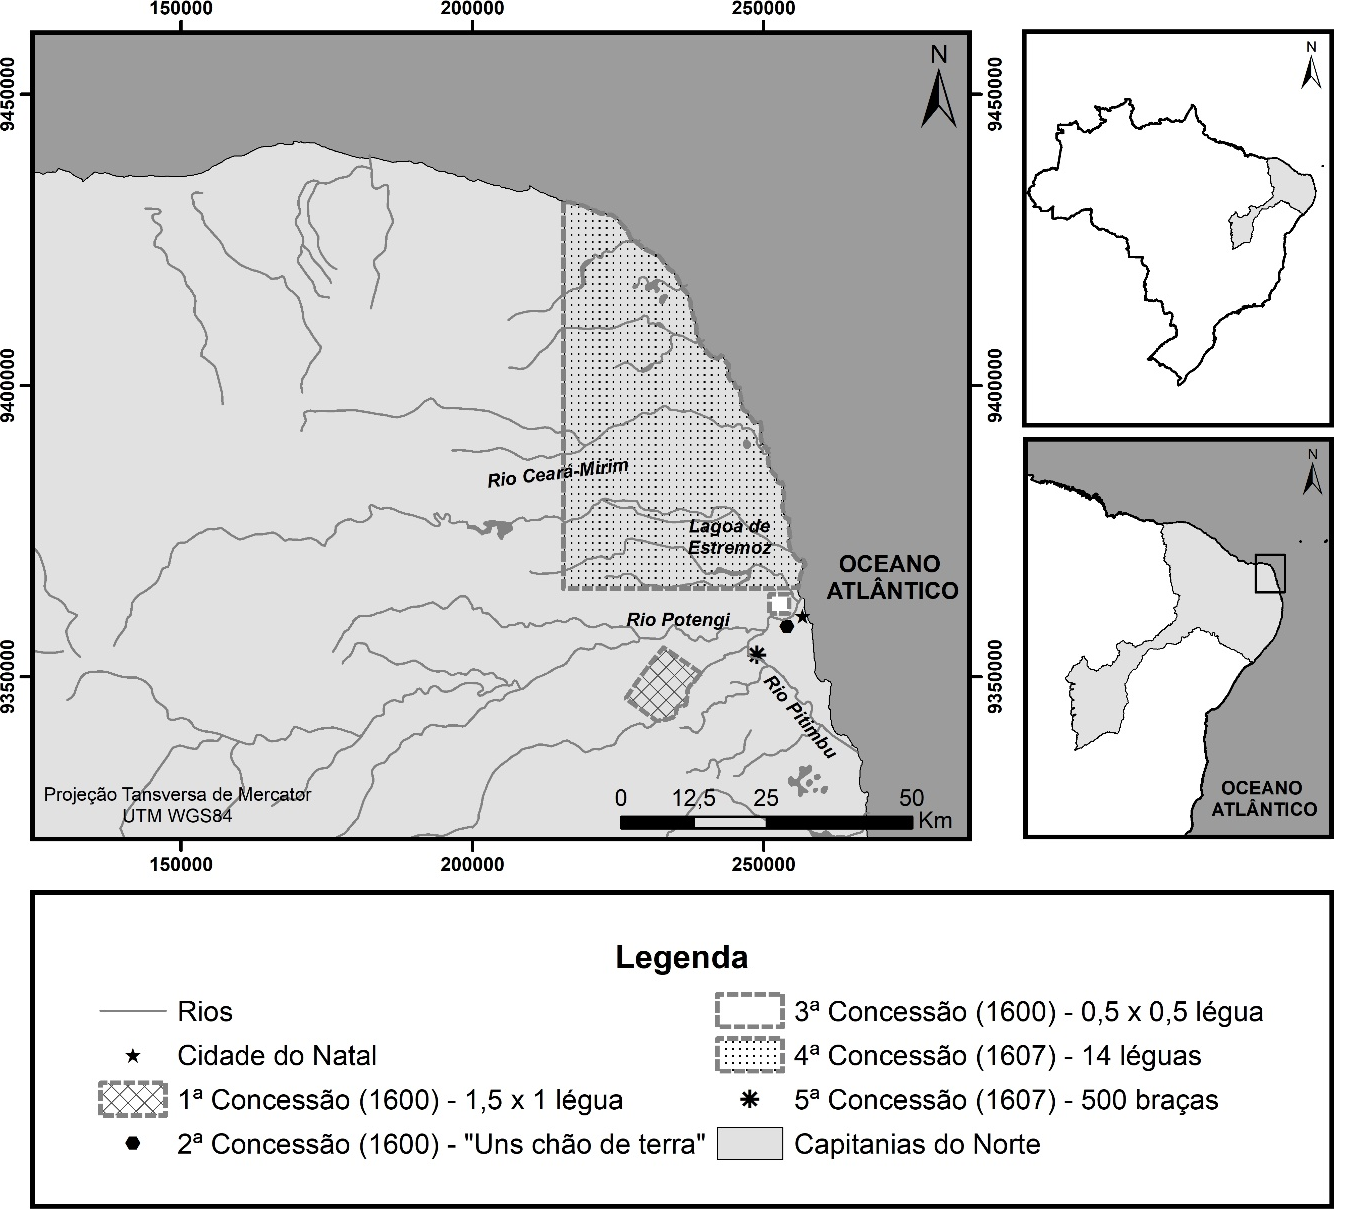
\includegraphics[width=1.05\textwidth]{articles/01-o-patrimonio-da-comp/fig01.png}%
    \caption*{Fonte: Elaboração própria a partir das informações contidas em: TRANSLADO, 1909.}%
    \label{fig:fig01}%
\end{figure}%

As outras duas datas de sesmarias foram concedidas pelo capitão-mor da capitania do Rio Grande, Jerônimo de Albuquerque, em 1607, e correspondem às datas número 102º e 103º do livro original de concessões. A primeira data localizava-se no “lugar chamado tijuru” (Guajiru), até o mar, podendo “compreender esta data quatorze léguas pouco mais ou menos”. Não há informações suficientes sobre os limites dessa sesmaria para realizar a sua delimitação, portanto, a área dessa concessão apontada na figura \ref{fig:fig01} é uma aproximação com base na extensão da mesma. Nessa sesmaria, a Companhia possuía dois currais de gado e quatro pessoas escravizadas originais da Guiné. A segunda data trata-se do aumento da primeira data de terra requerida pelos padres em 1600. Requereu-se os “sobejos que houvessem [de terras] que se achasse entre a data de Domingos Álvares e as dos padres”, sendo esta quinhentos braças --- equivalente a 1.100 metros, ou 0,16 légua em quadra --- de terras até chegar ao rio Pitimbu \cite[p.~49--51]{Translado1909}. 

Para Fátima Martins Lopes \citeyear[p.~107]{Lopes2003}, estas posses seriam a garantia do sustento dos padres da Companhia na capitania durante as missões volantes. O requerimento de um terreno na cidade do Natal fazia-se pela necessidade de os padres jesuítas formarem uma residência central, pois não havia muitos padres disponíveis, sendo impossível haver a quantidade necessária de padres para cada aldeia que deveria ser visitada. 

Ao requerer cinco datas de sesmaria, no entanto, tendo uma delas a grande extensão de 14 léguas, a Companhia de Jesus já deveria pensar sobre o crescimento da ordem na capitania do Rio Grande. Como foi explanado, as missões volantes eram periódicas e realizadas anualmente por apenas dois padres da Companhia. Assim, o requerimento de várias terras não representaria apenas a necessidade de garantir os mantimentos necessários para a subsistência dos padres na capitania. O exemplo das concessões de terra na capitania do Rio Grande aos inacianos corrobora as observações feitas pelos historiadores Edgard Leite \citeyear{Leite2000}, Paulo de Assunção \citeyear{Assuncao2004}, Maria Isabel da Silva Reis Vieira Rodrigues \citeyear{Rodrigues1997}, e Manoela Pedroza \citeyear{Pedroza2020} que atentaram para a ideia de que a Companhia de Jesus possuía a fé como justificativa para a ampliação de suas atuações. 

Cabe apontar que não se sabe o destino das terras concedidas aos jesuítas na capitania do Rio Grande na primeira década de 1600. O alvará de 1612 ordenou a diminuição da terra da Companhia do lugar chamado Tijuru, possivelmente Guajiru, nas proximidades da aldeia e lagoa de mesmo nome. Contudo, não se sabe o que aconteceu com as terras após a invasão holandesa e a fuga dos padres inacianos juntamente com outros moradores da capitania. Quando os inacianos retornaram à capitania do Rio Grande, depois de 1678, não há informações sobre a posse das terras doadas entre 1600 e 1607. Verificou-se, entretanto, que das cinco sesmarias doadas no início do século XVII encontrava-se nas posses da Companhia no momento de sua expulsão algumas fazendas de gado ainda localizadas na área de sesmarias de maior extensão.  

Fátima Martins Lopes \citeyear{Lopes2003} destacou que apesar das dificuldades enfrentadas pelos moradores na capitania, como a hostilidade dos índios e também pela natureza da região (falta de água, e solo arenoso), houve uma adequação às condições da capitania. Explorou-se o sal natural, foram criados gado e outros animais, desenvolveu-se pescarias e coletas de âmbar, e foram produzidos alimentos. A capitania do Rio Grande não possuía alfândega, assim não comercializava os seus produtos diretamente com Portugal, e sim por Pernambuco A capitania possuía apenas um engenho de cana-de-açúcar no período, o Cunhaú, não havendo uma produção de açúcar relevante. Além disso, é possível que pelo destaque na produção de alimentos, a capitania tenha comercializado internamente com as capitanias próximas, pois havia um livre comércio entre estas \cites[p.~191--196]{Dias2011}[p.~203--225]{Dias2018}. 

As terras requeridas pela Companhia podem ser associadas às atividades já referidas, pois se tratam de um sítio de salinas no litoral, ribeiras de rios importantes para currais de gado e cultivo de mantimentos. A presença de africanos escravizados em uma das concessões mostra o interesse dos jesuítas em iniciar uma atividade produtiva ou mesmo preparar e melhorar suas terras.  

Ao analisar o Translado do Auto de Repartição de Terras do Rio Grande, Lopes \citeyear[p.~103]{Lopes2003} observou que das 186 datas, apenas em sete havia referência sobre a presença de pessoas escravizadas nas terras, das quais apenas em duas fazia-se menção à posse de pessoas escravizadas da Guiné, sendo uma delas a da Companhia de Jesus. Segundo Lopes \citeyear[p.~68]{Lopes2003}, a escravidão negra no século XVII foi uma realidade para a Bahia e Pernambuco, capitanias açucareiras que podiam importar pessoas escravizadas, diferentemente do Rio Grande, onde a opção pela escravidão negra era muito restrita. Pesquisas mais recentes evidenciaram a presença da escravidão negra na capitania do Rio Grande somente para o final do século XVIII e início do século XIX \cites{Macedo2007,Souza2013}. Neste aspecto, a posse de pessoas escravizadas pela Companhia mostra que a ordem era privilegiada se comparada à situação dos demais moradores.  

Com a volta dos jesuítas à capitania após a expulsão dos holandeses, retomou-se o objetivo de catequizar os índios da região. Segundo Serafim Leite, “quebrando-se o julgo holandês, restabeleceu-se as atividades jesuíticas no Rio Grande, quer como feição econômica e rural, quer como a vida catequética nos aldeamentos de Guajiru e Guaraíras” \cite[Tombo~V,~p.~370]{Leite2004}. Dessa forma, além das atividades missionárias nos aldeamentos --- refere-se a um aglomerado resultante da “aculturação” mediante a presença de missionários catequistas \cite[p.~39]{Azevedo1957} --- os jesuítas também atuaram nas atividades econômicas da capitania.

Posteriormente à expulsão dos holandeses, as missões volantes ocorreram anualmente com a visita de dois padres do Colégio de Olinda da Companhia de Jesus. Atuaram formando alianças com os índios e batizando-os. Durante os contatos iniciais na capitania do Rio Grande, a habilidade intercultural dos jesuítas e o papel de intermediários, possibilitaram as alianças com os Potiguara. Os jesuítas tornaram-se mais eficientes que as forças militares, pois, possuíam melhores estratégias da aproximação, tendo possibilitado o encontro pacífico com os índios \cite[p.~88]{Porto2000}. 

Não há muitas informações acerca da atuação jesuítica na capitania do Rio Grande no período da ocupação holandesa (1633--1654). É sabido que até 1634, entretanto, os missionários visitaram algumas aldeias, mas após esta data, não há registro dos inacianos atuando na capitania \cite[p.~91]{Porto2000}. Com a expulsão dos holandeses, retomou-se o processo de colonização portuguesa na capitania: o Senado da Câmara de Natal foi restabelecido; as sesmarias passaram a ser doadas novamente; e posteriormente os jesuítas retornaram à capitania.  

Desde o Plano Civilizador do padre provincial Manuel da Nóbrega no governo de Mem de Sá, iniciou-se uma mudança na forma de catequizar os índios. Os jesuítas perceberam que a missão volante havia se tornado menos eficaz mediante a necessidade de melhor concentrar os índios e pregar a doutrina cristã, fazendo os índios abandonarem os seus hábitos culturais e tornarem-se cristãos. As missões efetivas, chamadas apenas de missões, aldeavam os índios buscando aproximar-se do ambiente natural dos mesmos, e simultaneamente visavam o seu afastamento dos centros de colonização \cite{Azevedo1959}. Tais missões também deveriam possuir uma organização administrativa, deveriam inserir os índios no trabalho agrícola, promover a ida à igreja, entre outras obrigações \cite[p.~162]{Lopes2003}. 

Este novo modo de catequizar os índios foi ao encontro dos interesses das autoridades da capitania, pois com a expulsão dos holandeses, a retomada da colonização na região expandiu-se para o interior, seguindo as frentes de penetração pecuária que provinham da Paraíba, Pernambuco e Ceará \cite[p.~129]{Lopes2003}. Ao direcionarem-se para o sertão --- aqui é compreendido como espaço sem atuação da Coroa portuguesa \cite[p.~112]{Silva2010} --- os colonos depararam-se com vários grupos indígenas, os quais foram resistentes à colonização portuguesa, gerando a Guerra dos Bárbaros \cites[p.~96]{Cascudo1984}{Dias2015}{Silva2015}.  

Neste contexto de conflitos entre índios e colonos e a necessidade de estender as posses de terras para a criação de gado, coube aos jesuítas aldear os índios para que estes fossem reduzidos em missões e fossem “apaziguados”. Nestas missões também se tentou regularizar a mão de obra indígena \cite[p.~95]{Porto2000}. 

Os jesuítas fixaram duas missões efetivas na capitania do Rio Grande. Ambos aldeamentos eram de remanescentes Potiguara, entre outras etnias: São Miguel de Guajiru e São João Batista das Guaraíras. O aldeamento de Guajiru estava localizado na margem da lagoa de mesmo nome (atual lagoa de Extremoz), a duas léguas da cidade do Natal, e foi relatada sua existência desde 1641, por um emissário holandês. Tal aldeamento, portanto, localizava-se na sesmaria de enorme extensão de 14 léguas concedida no início do século XVII a Companhia de Jesus. A presença dos jesuítas na aldeia foi mencionada a partir de 1679, por meio de uma queixa dos oficiais da Câmara da cidade do Natal ao bispo de Pernambuco, na qual acusavam o padre inaciano João de Gouveia de incitar os índios contra um administrador colonial. Entretanto, o primeiro relato oficial sobre a presença dos jesuítas na aldeia foi apenas em 1683, no Catálogo da Companhia de Jesus, sendo o seu superior o padre Antônio Cardoso, na qual também estava presente o padre Francisco de Albuquerque \cite[p.~170]{Lopes2003}.  

A presença jesuítica no aldeamento de Guaraíras, localizado nas proximidades do rio Jacu, foi relatada desde 1681, pois neste ano ordenou-se que os índios da aldeia de Mipibu fossem reunidos com os índios do aldeamento de Guaraíras \cite[p.~35]{Lemos1912}. A missão foi registrada nos Catálogos da Companhia de Jesus em 1683, com a presença do padre superior Luiz Pinto e do padre José dos Reis \cite[p.~172]{Lopes2003}.  

Foram nos aldeamentos de Guajiru e Guaraíras, e em suas proximidades, que a Companhia de Jesus exerceu as suas atividades de forma mais intensa. Ao fundar uma missão fixa, os jesuítas deveriam preocupar-se com o sustento da ordem, bem como de seus membros e dos índios. Houve a necessidade da fundação de fazendas para a produção de mantimentos, e criação de animais. A forma como os jesuítas administravam as atividades produtivas nos aldeamentos e em suas fazendas, pode ser percebida por meio da análise de suas posses de terra e dos conflitos derivados desta prática.  

Com o Alvará de 23 de novembro de 1700, que garantiu uma légua de terra em quadra (uma légua -- 6,6 km -- de comprimento por uma de largura) para o sustento dos índios e missionários, as missões Guajiru e Guaraíras tiveram suas terras demarcadas na primeira década do século XVIII \cites[p.~111--112]{Cascudo1984}[p.~44]{Lopes2005}.  

Além das terras das missões, que pertenciam aos índios nelas aldeados, mas que também eram usufruídas pelos inacianos, observou-se por meio de algumas cartas de sesmarias que apontavam os jesuítas como confrontantes de suas terras, que a Companhia de Jesus possuía outras terras na capitania do Rio Grande.   

Antônio Cardoso Batalha solicitou uma terra nas proximidades da ribeira do Ceará-Mirim, em 1739, e afirmou que a terra chamada Maracacheta, localizada nas proximidades do rio Ceará-Mirim, em direção à praia (litoral leste da capitania) pertencia aos Jesuítas.\footnote{Instituto Histórico e Geográfico do Rio Grande do Norte [IHGRN] --- Fundo Sesmarias, Livro IV, n. 287, fl. 51--52.} Acredita-se na possibilidade de o lugar Maracacheta ter alguma relação com o lugar chamado Massangana, localizado ao norte da missão de Guajiru.  

O padre jesuíta Antônio de Amorim, em agosto de 1736, requereu um novo documento da sesmaria que herdou de seu pai, o coronel Antônio Dias Pereira. A petição foi feita por intermédio do procurador do suplicante, o padre jesuíta coadjutor e licenciado João Gomes Freire. A terra requerida localizava-se nas confrontações das terras da própria Companhia de Jesus, nas proximidades do rio Ceará-Mirim, seguindo o curso do rio Caratã --- hoje rio Mudo, ou rio do Jorge, o qual deságua na lagoa de Extremoz, antiga lagoa de Guajiru \cite[p.~79]{Cascudo1968} --- ficando este no meio das terras de um lugar chamado Cacimbas.\footnote{IHGRN --- Fundo Sesmarias, Livro III, n. 241, fl. 158--159.} Esta sesmaria pode revelar não apenas uma terra da Companhia nas proximidades da missão de Guajiru, como também pode evidenciar a anexação da terra herdada por um membro da Companhia, visto que quem realizou a petição foi outro padre jesuíta e a terra localizava-se nas confrontações de outras terras da ordem. Ao catequizar os índios nas ditas missões, os jesuítas utilizaram-se das terras das mesmas, bem como das terras que haviam requerido inicialmente para as fazendas que produziam mantimentos e tinham criações de gado para efetivar a catequização.  

Para a identificação das posses jesuíticas na capitania do Rio Grande na primeira metade do século XVIII realizou-se a análise de fontes referentes ao estabelecimento do Diretório dos Índios. Esse, decretado em 8 de maio de 1758, aboliu o poder temporal e espiritual dos missionários sobre os índios aldeados. Desta forma, os inacianos deveriam ser substituídos pela administração civil e pelo clero secular \cite[p.~18--20]{Couto1990}. Em 14 de setembro do mesmo ano, Luís Diogo Lobo da Silva, governador das Capitanias do Norte, ordenou que fossem erigidas vilas nos aldeamentos administrados pelos jesuítas \cite[p.~43--46]{Couto1990}. No início do ano de 1759, Dom Francisco Xavier Aranha, bispo de Pernambuco, ordenou aos superiores dos Colégios de Olinda e Recife, que quando os substitutos seculares chegassem às missões os jesuítas deveriam se retirar das mesmas e se dirigissem aos seus Colégios \cite[p.~102]{Lopes2005}. 

Em junho de 1759, os párocos seculares chegaram às missões do Rio Grande, e realizou-se um alistamento dos bens pertencentes às missões, às igrejas e às residências jesuíticas. Os bens móveis dos jesuítas passaram a ser subordinados à jurisdição do arcebispo de Olinda, visto que seu caráter religioso impedia que a Coroa os confiscasse. Assim, o rei permitiu que tais bens ficassem sob a responsabilidade do arcebispo de Olinda, o qual deveria sequestrar e repartir tais bens \cite[p.~29--35]{Couto1990}. O ouvidor geral Bernardo Coelho da Gama e Casco ordenou que se realizasse o inventário dos bens das missões jesuíticas da capitania do Rio Grande, Guajiru e Guaraíras, em 1760, os quais foram registrados em 1761 \cite[p.~172]{Lopes2005}. 

O padre inaciano Alexandre Carvalho entregou os bens da igreja da antiga missão de Guajiru, Nossa Senhora dos Prazeres e São Miguel, para o vigário Antônio de Souza Magalhães. No inventário, que se encontra no códice 1964 do Arquivo Histórico Ultramarino (AHU), os bens da igreja eram compostos por 17 imagens religiosas, das quais sete apresentavam adornos de prata, e uma de ouro; vários objetos destinados para a celebração de missas, dos quais alguns eram de prata como relicários, vasos de comunhão, cálices e turíbulo; toalhas, cortinas, mantos, capas, véus, missais, entre outros. A construção da igreja de Nossa Senhora dos Prazeres e São Miguel ainda não estava concluída no momento do inventário.\footnote{Arquivo Histórico Ultramarino [AHU] --- Códice 1964, fl. 337--342. Inventário que mandou fazer o Dr. Desembargador ouvidor geral Bernardo Coelho da Gama e Casco, de Todos os Bens Pertencentes a esta missão de Guajiru e igreja de Nossa Senhora dos Prazeres e São Miguel.} 

A missão de Guajiru possuía 70 cabeças de gado vacum e nove de cavalar. Também possuía 15 pessoas escravizadas.\footnote{AHU --- Códice 1964, fl. 337--342.} Como os missionários não possuíam comprovantes da origem da posse pessoas escravizadas, nem de seus gados, o ouvidor geral da Gama e Casco instaurou um sumário de testemunhas para que fosse apurado se estas propriedades pertenciam à missão ou à Companhia de Jesus. Segundo alguns índios, antigos moradores da missão, as pessoas escravizadas eram descendentes dos cativos que os missionários haviam comprado ou trazido nos primórdios da missão.\footnote{AHU --- Códice 1964, fl. 343--347. Auto de Sumário que mandou fazer Bernardo Coelho da Gama e Casco para por ele perguntar testemunhas ex-ofício, em 30/05/1760.} 

Na missão de Guaraíras, os bens foram passados ao vigário Pantaleão da Costa de Araújo pelo padre jesuíta Manoel Pinheiro. A igreja de São João Batista encontrava-se nova, construída de pedra e cal. Os bens pertencentes a esta igreja, embora possuíssem menos imagens religiosas com adornos de prata em comparação à missão de Guajiru, possuía mais bens. Havia pias de água benta, pia batismal, dois confessionários, e ainda uma grande variedade de utensílios religiosos e adornos decorativos: galhetas, cruzes, cálices de prata, castiçais, velas, bandeiras de paniconografia (gravura em relevo sobre zinco), e panos, mantos, cortinas e vestimentas sacerdotais de tecidos nobres. A missão ainda possuía 174 cabeças de gado vacum, 57 de cavalar, 27 de gado caprino, 38 de ovino, três porcos, e mais vinte e três mil e setecentos réis.\footnote{AHU --- Códice 1964, fl. 390--398. Inventário que mandou fazer o Dr. Desembargador ouvidor geral Bernardo Coelho da Gama e Casco, de todos os bens pertencentes a esta missão de guariras e igreja de São Sebastião.}  

A missão de Guaraíras possuía pertences que podem refletir uma melhor condição dessa missão em comparação à missão de Guajiru. A missão de Guaraíras possuía uma livraria com 20 volumes, e interessantes utensílios como “uma chocolateira e seu pau”, um “baú de Moscóvia”, e “umas charamelhas” (instrumento de sopro).\footnote{AHU --- Códice 1964, fl. 390--398.} 

Ambas as residências das missões possuíam uma mobília básica como cadeiras, mesas, tamboretes, e objetos de higiene pessoal. Em ambos os inventários também se percebe instrumentos de trabalho, relacionados à produção econômica desempenhada pelos índios, como redes de pescas, serrotes, entre outros \cite[p.~173]{Lopes2005}. 

Assim, como havia sido acordado anteriormente, desde maio de 1758, os bens semoventes (ornamentos, utensílios, animais, pessoas escravizadas, entre outros) das missões jesuíticas foram divididos em 1761, conforme a proposta lançada pelo bispo de Olinda à junta criadora das vilas, que incluía representantes eclesiásticos, funcionários coloniais e índios que ocupavam cargos civis e militares \cite[p.~179]{Lopes2005}. Os bens de raiz das missões, ou seja, as terras que foram concedidas para a criação da missão ou mesmo para a ampliação de sua extensão, deveriam ser repartidas entre os índios das mesmas de acordo com o arcebispado, e o governador ou capitão-mor da capitania, não ficando nenhuma terra para a igreja.\footnote{Arquivo Público do Estado de Pernambuco [APEPE] --- Ordens Régias, Livro nº 10 (1755--1760), fl. 144--146. }

As providências para erigir as novas vilas começaram no início do ano de 1759. As missões de Guajiru e de Guaraíras tornaram-se respectivamente as vilas de Estremoz em 3 de maio de 1760, e a vila de Arêz em 15 de junho de 1760 \cite[p.~122--123]{Lopes2005}. Nesta mudança de missões para vilas, também foi ordenado que o ouvidor geral Bernardo Coelho da Gama e Casco convocasse os prelados dos Colégios de Olinda (ao qual estavam submetidas às missões jesuíticas do Rio Grande), Recife e Paraíba, para que fossem apresentados os bens que os jesuítas possuíam em um prazo de 20 dias após a averiguação e levantamento dos bens.\footnote{APEPE --- Ordens Régias, Livro nº 10 (1755--1760), fl. 144--146.} 

Desde maio de 1758, o rei havia ordenado que os bens de raiz pertencentes à Companhia de Jesus que estivessem em desacordo com as antigas leis impostas a ordens religiosas poderiam ser sequestrados. Assim, os bens de raiz que não possuíssem licença régia --- norma referente ao Título XVIII das Ordenações Filipinas, presente no alvará de 30 de julho de 1611, no qual se ordenou que todos os bens religiosos deveriam possuir sua respectiva autorização --- poderiam ser de imediato revertidos à Coroa portuguesa. Em agosto de 1759, o rei Dom José ordenou que fosse realizado o sequestro de todos os bens da Companhia de Jesus em Pernambuco com sua respectiva origem e valor.\footnote{Arquivo Nacional da Torre do Tombo [ANTT] --- Documentação das capitanias do Brasil existente no núcleo do Real Erário, Livro nº 574, documento sem número. }

Assim, averiguaram-se alguns bens de raiz da Companhia de Jesus na capitania do Rio Grande pertencentes então ao Colégio de Olinda. O ouvidor Gama e Casco arrolou alguns bens de raiz e os colocou em arrematação pública para serem arrematados em 1º de junho de 1760 --- a saber as fazendas: Oitizeiro, Ceará e Curral de Baixo.\footnote{AHU-PE --- Papéis Avulsos, Cx. 95. Doc. 7493. Ofício do ouvidor geral Bernardo Coelho da Gama e Casco ao secretário de Estado Conde de Oieiras. 10 de fevereiro de 1761.} É sabido que além dessas fazendas os inacianos possuíam na capitania do Rio Grande os sítios Galos e Guamaré e uma fazenda de gado chamada de Santa Cruz,\footnote{AHU-PE --- Papéis Avulsos, Cx. 95. Doc. 7493.} como se pode ver na figura \ref{fig:fig02}.  

Segundo José Jorge da Costa Couto, enquanto Portugal negociava com a Cúria de Roma (1759-1760) acerca da situação dos bens jesuíticos, a administração de Portugal manteve os bens fundiários da ordem jesuítica intocáveis, com exceção dos bens que não possuíam licença régia \cite[p.~149]{Couto1990}.   

Com a definitiva expulsão dos jesuítas de Portugal e de todos os seus domínios, em 3 de setembro de 1759, os bens da Companhia de Jesus foram revertidos à Coroa, visto que a ordem religiosa foi extinta. Tal fato foi corroborado pelo alvará de 25 de fevereiro de 1761, o qual determinou a imediata incorporação no fisco da Câmara Real de todos os bens temporais, isto é, aqueles que não se encontravam direta e exclusivamente destinados ao culto divino \cite[p.~151]{Couto1990}. 

Desse modo, a ordem régia de 22 de outubro de 1761 estabeleceu como os bens confiscados dos jesuítas deveriam ser classificados, registrados e arrematados. Os bens imóveis deveriam ser alienados em público, com a presença da Junta congregada, sendo aceito o maior lance dos sujeitos interessados em arrendar o bem. A arrematação poderia ser paga em dinheiro ou em gêneros de fácil venda \cite[p.~153]{Couto1990}. As normas da referida ordem chegaram ao governador de Pernambuco, e consequentemente para as Capitanias do Norte, apenas em 1763. 

\begin{figure}[ht]%
    \centering%
    \caption{As terras da Companhia de Jesus na data de sua expulsão (1759)}%
    \hspace*{-.025\textwidth}
    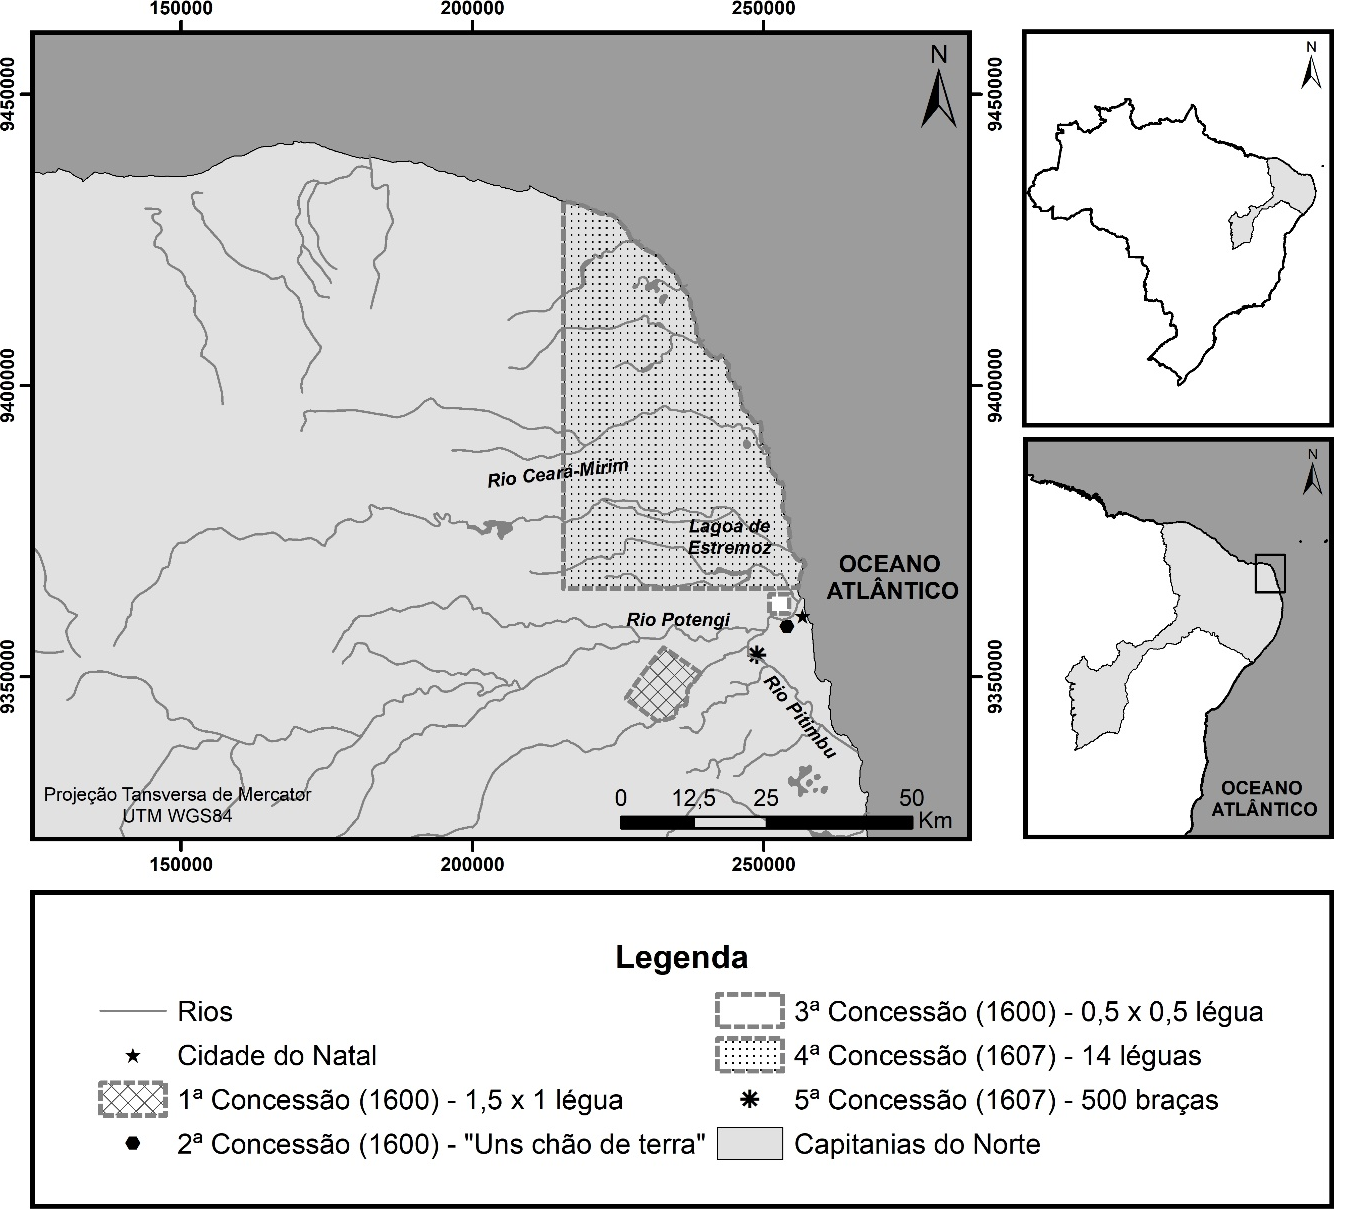
\includegraphics[width=1.05\textwidth]{articles/01-o-patrimonio-da-comp/fig01.png}%
    \caption*{Fonte: Elaboração própria a partir das informações contidas em: IHGB --- Arq. 1.1.15. Avaliações dos bens jesuítas em Pernambuco, 1772. AHU-PE --- Papéis Avulsos, Cx. 95. Doc. 7493. 10 de fevereiro de 1761. }%
    \label{fig:fig02}%
\end{figure}%

Foi criada, em 10 de abril de 1769, uma Junta da Fazenda Real em Pernambuco, para evitar falhas na administração e arrecadação da Real Fazenda de Pernambuco. A mesma era composta pelo governador, procurador, provedor e contador da Fazenda. A Junta deveria ser responsável por classificar os bens confiscados bem como elaborar um livro de inventário dos ditos bens \cite[p.~158]{Couto1990}. 

Foi por meio destes documentos produzidos pela Junta da Fazenda Real em Pernambuco que é sabido que, em 1772, algumas fazendas jesuíticas no Rio Grande, pertencentes ao Colégio de Olinda, não estavam arrematadas: fazenda Oitizeiro; fazenda Ceará; fazenda Curral de Baixo; sorte de terras no lugar chamado Ceará; e sítio de terra chamado Arraial das Formigas na ribeira do rio Piranhas.\footnote{Instituto Histórico e Geográfico Brasileiro [IHGB] --- Arq. 1.1.15. Avaliações dos bens jesuítas em Pernambuco, 1772, p. 9--11.} 

As fazendas Oitizeiro, Ceará, e Curral de Baixo, as quais haviam sido arrematadas a Antônio da Silva de Carvalho em 1760, ficaram deterioradas após o falecimento do mesmo. As ditas três fazendas passaram novamente para a administração da Provedoria da Fazenda do Rio Grande, em 1770, e foram leiloadas em 1776 para Domingos Gomes Maciel.\footnote{ANTT --- Erário Régio, Capitanias do Brasil --- Pernambuco, livro 636, traslado nº 3, Autos de arrematação dos bens confiscados dos jesuítas e pertencentes ao Fisco Real, dos anos de 1776, 1777 e 1778. Em carta da Junta de Pernambuco, de 15 de junho de 1779.}  

As posses de terras da Companhia de Jesus na capitania do Rio Grande as quais se tem conhecimento foram as fazendas Oitizeiro, Ceará, Curral de Baixo e Santa Cruz; os sítios dos Galos, Guamaré, e o Arraial das Formigas; além de uma sorte de terra no lugar chamado Ceará; totalizando três fazendas, dois sítios, um arraial e uma sorte de terra. Como os bens imóveis citados, referentes às missões de Guajiru e Guaraíras, estavam subordinados a mesma jurisdição do Colégio jesuítico de Olinda, não se conseguiu verificar por meio da documentação analisada quais fazendas estavam subordinadas à administração específica dos padres da missão de Guajiru, com exceção da fazenda Santa Cruz.\footnote{AHU --- Códice 1822, fl. 31v--32, CARTA do capitão-mor do Rio Grande, João Coutinho de Bragança ao governador de Pernambuco, em 17/02/1760.}

\section{Os bens como sustento da fé}

Segundo o historiador Fabricio Lyrio Santos \citeyear{Santos2008} as práticas inacianas de acumulação de bens não contradiziam o voto de pobreza dos membros da ordem. Essa concepção acerca da acumulação de bens para o desenvolvimento das atividades da ordem inaciana estava presente já na versão sumária das regras de funcionamento da ordem, aprovada pelo Papa Paulo III em 1540, na qual o fundador da Companhia de Jesus, padre Inácio de Loyola, recomendava o voto de pobreza, mas, permitia que se aceitassem rendas para o sustendo dos estudantes \cite{Santos2008}.  

Além disso, as cartas apostólicas \textit{Regimini militantis Ecclesiae}, de 27 de setembro de 1540, e \textit{Exposcit debitum}, de 21 de julho de 1550, corroboravam as regras de criação da ordem e aceitavam que a mesma estabelecesse colégios para formação de estudantes e novos membros da ordem. Tais colégios deveriam possuir suas próprias rendas e/ou propriedades para sua manutenção e sustento de seus membros \cite{Santos2008}. Portanto, poderiam ou deveriam ser aceitas as doações régias para efetivar o funcionamento da ordem jesuítica.  

Segundo Edgard Leite \citeyear[p.~60]{Leite2000}, a história da Companhia de Jesus no Brasil é a história da construção de um gigantesco patrimônio, o qual foi construído por uma série de privilégios e favorecimentos da Coroa portuguesa, e também por decisão acordada dentro da própria ordem. 

Desde o primeiro ano que os jesuítas chegaram ao Brasil, em 1549, receberam benefícios, bem como muitos colonos \cite[p.~30--71]{Fragoso2001}. No dito ano, a bula papal \textit{Licet Debitum} isentou o pagamento de dízimos \cite[Tombo~VII,~p.~103]{Leite2004}. Tal isenção foi confirmada no reinado de Dom Sebastião posteriormente em 1576 e 1577. Também foi estabelecido, desde o princípio das ações jesuíticas, o fornecimento de gêneros à Companhia, com finalidade de manter as necessidades da ordem. A partir de 1560 e 1570, uma porcentagem dos impostos arrecadados pagos em açúcar à Coroa, a redízima dos dízimos, era repassada aos três colégios jesuíticos do Brasil: Bahia, Rio de Janeiro e Olinda. Em 1573, um alvará isentou a Companhia dos pagamentos de direitos alfandegários sobre os produtos que recebessem na ou enviassem da América portuguesa. A Coroa também destinava aos jesuítas a subvenção pessoal, equivalente a uma pensão anual, para aqueles que embarcavam de Portugal para o Brasil, sendo 20.000 réis em 1581, e 35.000 réis em 1690 \cite[p.~60--61]{Leite2000}. 

Além dos subsídios reais, com a reconhecida necessidade da posse de terras para o sustento da ordem jesuítica, bem como para a formação de núcleos territoriais, os membros da Companhia obtiveram terras por meio das seguintes formas: sesmaria, doação, compra, e mais raramente a troca \cite[p.~12]{Alveal2002}. As doações de fiéis podiam ocorrer pela estipulação de um valor a ser doado à Companhia anualmente, em espécie ou em produtos do mercado colonial \cite[p.~81]{Assuncao2004}. 

Os subsídios reais e as isenções de pagamentos de dízimos e taxas alfandegárias mostraram o interesse da Coroa portuguesa de livrar a ordem de obrigações, proporcionando não apenas o seu mantimento, como também o seu crescimento. Para a Coroa, a presença jesuítica, naquele momento, era não apenas favorável como necessária, pois, convertia-se o gentio e controlava-se a mão de obra indígena, combatia-se a ação de invasores estrangeiros e relatava-se a presença destes, e, sobretudo, confirmava a presença portuguesa no novo território \cite[p.~156]{Assuncao2004}. Assim, esse importante papel da Companhia de Jesus na integração do mundo colonial era percebido como um serviço prestados à Coroa. 

Ao descrever sobre os bens da Companhia, o historiador e padre jesuíta Serafim Leite relatou que, à primeira vista, os bens da Companhia geram uma visão equivocada da ordem. Ele afirma que o equívoco é desfeito quando percebida a necessidade dos bens para a manutenção da Companhia. Segundo o autor, os jesuítas não obtinham lucros das atividades que exercitavam, apenas necessitavam de maiores subsídios para continuarem com as atividades missionárias \cite[Tombo~I,~p.~49]{Leite2004}.

Assim como Serafim Leite, Dauril Alden não corrobora a ideia de que a Companhia de Jesus se utilizou do comércio e de outras estratégias para manter a ordem religiosa. Ambos os autores afirmam que a Companhia não havia quebrado o voto de pobreza. Alden defende que a Companhia de Jesus não obteve ganhos significativos, e contesta a associação entre jesuítas e homens do comércio moderno, comumente realizada. Para Alden \citeyear[p.~527]{Alden1996}, as atividades desenvolvidas pela Companhia não se enquadravam como comércio.  

Entretanto, autores como Paulo de Assunção \citeyear{Assuncao2004}, Edgard Leite \citeyear{Leite2000}, Maria Isabel da Silva Reis Vieira Rodrigues \citeyear{Rodrigues1997} e Manoela Pedroza \citeyear{Pedroza2020}, demonstraram por meio de suas pesquisas que a Companhia de Jesus possuía a fé como justificativa para a ampliação de suas atuações, principalmente no comércio de gêneros alimentícios. Por meio do apoio da Coroa, de concessões de terras, das doações de fiéis, e da administração de seus bens, a Companhia construiu no Brasil um grande e poderoso patrimônio.   

Os jesuítas, inseridos em uma sociedade colonial em formação, acabaram por se adequar àquela sociedade. A mentalidade moderna do descobrimento e da conquista não influenciou apenas a monarquia e os colonos. Os jesuítas, ao compartilharem um mesmo espaço de relações sociais, incorporaram valores modernos em suas atuações, tornando-se necessário para o desenvolvimento da ordem, a inserção dos jesuítas no mundo mercantilista \cite[p.~239]{Assuncao2004}. Deste modo:

    \begin{quote}
    A preocupação com o cultivo e a exploração das terras de forma a garantir a estrutura da Companhia colocou-a em consonância com a lógica da colonização da época moderna. O empreendimento jesuítico era parte de uma ação colonizadora que almejava, por meio da circulação de mercadorias, efetivar o poder da fé. \cite[p.~251]{Assuncao2004}         
    \end{quote}

Os jesuítas designados a missionar na América portuguesa encontravam-se inseridos em um novo mundo que, diferentemente do contexto europeu, havia necessidades e dificuldades específicas reveladas pelo meio: a produção de alimentos, as pragas e pestes nos roçados, guerras entre etnias indígenas, invasões estrangeiras, entre outras. Mesmo com os subsídios e doações reais, a Companhia de Jesus encontrava-se desprovida, insegura, sendo necessária a incorporação dos valores da época moderna para que superassem as dificuldades e mantivessem as atividades missionárias e o crescimento da ordem \cite[p.~151]{Assuncao2004}. 

Cabe ressaltar que propriedade está relacionada à mentalidade, ou seja, a forma como se compreendia a posse de uma terra estava associada aos valores dos indivíduos que o fazia. Dessa forma, as concepções acerca da posse de terras devem ser relativizadas, pois o vínculo de um sujeito ou instituição com a terra está relacionada à sua concepção de mundo \cite[p.~30--31]{Grossi2006}. Além disso, negar a necessidade da produção de mantimentos, bem como a preocupação com o sustento da ordem, seria negar as condições adversas existentes no novo mundo colonial que, principalmente no século XVI e XVII, dificultou a ação dos colonizadores e também dos religiosos. Portanto, a posse de terras deve ser compreendida como necessária para a existência de indivíduos e de instituições na América portuguesa, embora, as percepções acerca destas posses fossem diferentes entre si.  

Ao longo da atuação da Companhia de Jesus no Brasil construiu-se um vultuoso patrimônio por meio dos favorecimentos e privilégios reais, doações, concessões de terras, e pelo bom gerenciamento de suas atividades. A Companhia de Jesus, contudo, ao efetivar seus objetivos de converter os indígenas e gerar o sustento da ordem, além de manter um domínio espiritual sobre os colonos, construiu articulações políticas e econômicas. O crescente poder dos inacianos foi uma das muitas motivações da Coroa portuguesa para a expulsão dessa ordem de todos os seus territórios \cite{Couto1990}.



\section{Conclusão}

A presença jesuítica na colonização da capitania do Rio Grande do Norte, bem como da América portuguesa, era necessária, pois, convertia-se os índios e controlava-se sua mão de obra, combatia-se a ação de invasores estrangeiros e relatava-se a presença destes, e, principalmente, afirmava a presença portuguesa no novo território. Assim, pode-se afirmar que o empreendimento jesuítico na capitania era parte de uma ação colonizadora que almejava efetivar o poder da fé por meio da consolidação de um sólido patrimônio e da circulação de mercadorias. Por sua vez, a construção do patrimônio jesuítico foi viabilizada pelo apoio da Coroa, com a larga concessão de terras, e, possivelmente, das doações de fiéis.

\printbibliography[heading=subbibliography,notcategory=fullcited]

\hfill Recebido em 07 abr. 2021

\hfill Aprovado em 24 abr. 2021

\label{chap:patrimonioend}

\end{refsection}

\begin{refsection}
\renewcommand{\thefigure}{\arabic{figure}}

\chapterTwoLines
{Farinha e carne no sertão. Fome e carestia no litoral}
{aspectos do mercado interno no Rio Grande do Norte (séc. XVIII a XIX)}
\label{chap:farinha}

\articleAuthor
{Thiago Alves Dias}
{Doutor pelo Programa de Pós-Graduação em História Econômica da Universidade de São Paulo (PPGHE/USP), professor de História Moderna na UPE e pesquisador no grupo de pesquisa do CNPq ``Laboratório de Experimentação em História Social'' da UFRN. ID Lattes: 4789.9607.6279.7571. ORCID: 0000-0003-4308-418X. E-mail: thiago.dias@upe.br.}

\begin{galoResumo}
    \marginpar{
        \begin{flushleft}
        \tiny \sffamily
        Como referenciar?\\\fullcite{SelfDias2021}\mybibexclude{SelfDias2021}, p. \pageref{chap:farinha}--\pageref{chap:farinhaend}, \journalPubDate{}
        \end{flushleft}
    }
    Partindo da análise de dois gêneros básicos da alimentação colonial que foram objetos de regulação direta das instituições administrativas coloniais, a farinha de mandioca e a carne bovina, o presente artigo visa contribuir com a escassa discussão historiográfica norte-rio-grandense sobre o mercado interno e as dinâmicas mercantis coloniais durante o século XVIII e primeira metade do XIX, notadamente, da cidade do Natal. Com base nos registros da Câmara de Natal, cartas de sesmarias e outras fontes documentais, bem como amparado nas proposituras teóricas do historiador econômico Istvan Hont, concluímos que o comércio interno no Rio Grande do Norte, em geral, e na cidade de Natal, em particular, ganhou conjunturas de estabilidade e superação de problemas de abastecimento a partir da conquista colonial dos sertões e das prerrogativas institucionais de controle auferidas pela Câmara de Natal.
\end{galoResumo}

\galoPalavrasChave{Câmara de Natal. Rio Grande do Norte. Mercado interno.}

\begin{otherlanguage}{spanish}

    \fakeChapterTwoLines
    {Harina y carne en el sertão. Hambre y carestía en la costa}
    {aspectos del mercado interno en Río Grande del Norte (siglos XVIII al XIX)}
    
    \begin{galoResumo}[Resumen]
        Desde el análisis de los tipos básicos de alimentos coloniales que fueron objeto de regulación directa por parte de las instituciones administrativas coloniales, la harina de mandioca y la carne vacuna, este artículo tiene como objetivo contribuir a la escasa discusión historiográfica en el mercado interno de Río Grande del Norte y la dinámica mercantil colonial durante el siglo XVIII y la primera mitad del XIX, especialmente en la ciudad de Natal. Basándose en los registros de la Cámara de Natal, cartas de sesmarias y otras fuentes documentales, así como amparado en los planteamientos teóricos del historiador económico Istvan Hont, concluimos que el comercio interno en Río Grande del Norte, en general, y en la ciudad de Natal, en particular, ganó estabilidad y superó problemas de abastecimiento como resultado de la conquista colonial del interior y de las prerrogativas institucionales de control obtenidas por la Cámara de Natal.
    \end{galoResumo}
    
    \galoPalavrasChave[Palabras clave]{Cámara de Natal. Río Grande del Norte. Mercado interno.}
\end{otherlanguage}

\section{Introdução}

No mês de julho de 1711, a Câmara de Natal registrou em seus livros a falência de João do Rosário, o contratador das carnes daquele ano. Resolveram, portanto, notificar o fiador do contrato, o tenente-coronel e vereador Manoel Rodrigues Coelho, exigindo que o mesmo apresentasse uma solução para o caso. Naquela altura, Manoel Rodrigues Coelho já estava de volta a Natal, já que o mesmo estava nas trincheiras do Assú combatendo com os indígenas do sertão, sendo inclusive eleito no ano de 1712 a função de Juiz Ordinário da Câmara de Natal. Ocorre que durante o mês de junho daquele ano de 1711, mês festivo em torno do fim da colheita do milho e apropriado pelo calendário cristão em memória dos santos Antônio, João e Pedro; a cidade sofreu um verdadeiro desabastecimento de carne bovina\footnote{Instituto Histórico e Geográfico do Rio Grande do Norte [IHGRN] --- Livros de Termos de Vereação da Câmara de Natal [LTVCN], livro 1709--1721. Câmara de Natal. Termo de Vereação de 02 de julho de 1711, fl. 43v. Manuscrito.}.

No mês de maio de 1713, ou seja, em meio ao problema do abastecimento da carne bovina, a Câmara de Natal decidiu, acatando a queixa da população, instituir uma multa para os agricultores que fabricavam farinha de mandioca e não traziam para a venda pública na cidade do Natal\footnote{IHGRN --- LTVCN, livro 1709--1721. Câmara de Natal. Termo de Vereação de 23 de maio de 1713, fl. 77v-78. Manuscrito.}. Muito embora não houvesse impostos diretos da Câmara sobre a comercialização da farinha de mandioca, o que poderia encarecer o produto, como era o caso da carne bovina, a oferta do ``ordinário pão da terra'', como referiu-se Francisco de Brito Freire em 1630 \cite[p.~187]{Freire1675nova} e reiterado por Caio Prado Jr. em suas relevantes proposituras sobre a agricultura de subsistência no Brasil colonial \cite[p.~165]{PradoJr1997}, também sofria com as guerras no sertão. O abastecimento das tropas do Açu impedia que a produção de farinha do sertão viesse para o litoral. Além disso, parte considerável da farinha produzida no litoral seguia o lucrativo comércio com a capitania de Pernambuco, problema essa que teve continuidade durante todo o século.

Esse quadro de guerras coloniais contra os indígenas e a oferta de mercados mais vantajosos fora da Capitania do Rio Grande do Norte, provocou sucessivas ondas de desabastecimento na cidade de Natal durante o século XVIII: nem carne, nem farinha.

O presente artigo visa contribuir com a escassa discussão historiográfica norte-rio-grandense sobre o mercado interno e às dinâmicas mercantis coloniais durante os séculos XVIII e XIX, notadamente, da cidade do Natal. A problemática aqui discutida limita-se entre o fim das Guerras de Conquista do Sertão, a chamada ``Guerra dos Bárbaros'' (c. 1720), até, aproximadamente, a segunda metade do século XIX, quando a cotonicultura muda, drasticamente, os padrões de consumo e de circulação de produtos do comércio interno no Rio Grande do Norte.  

No tocante a historiografia, diferentes esforços de pesquisas em história econômica e social do Brasil, notadamente, a partir da década de 1970, tem se debruçado sobre as formas de organização e funcionamento dos circuitos mercantis internos no período colonial \cites{Linhares1979historia}{Lapa1980modos}. Passado mais de meio século, a crescente preocupação das humanidades com problemáticas permanentes, tais como: acesso à terra, desiguais relações de trabalho e ausência de políticas públicas de financiamento e intervenção estatal em áreas produtivas estratégicas, por exemplo, continuam conduzindo a comunidade acadêmica a investigar o nosso passado agrário. Essas pesquisas têm o mérito de buscar evidenciar, entre outras questões, as práticas comerciais endógenas e aspectos da economia de subsistência na América portuguesa, passando pela formação e consolidação de mercados internos. Esse esforço contínuo de produção de conhecimento visa nos auxiliar, enquanto sociedade, na definição de caminhos e estratégias para superação de parte desses nossos problemas históricos. 

Esse artigo partiu da análise de dois gêneros básicos da alimentação colonial que foram objetos de regulação direta das instituições administrativas coloniais: a carne bovina e a farinha de mandioca. A escolha deve-se ao fato de que inicialmente esses gêneros foram largamente produzidos no litoral atendendo as demandas populacionais proporcionais ao primeiro século da colonização. Com o adensamento populacional litorâneo, a consolidação da conquista dos sertões na primeira metade do século XVIII, foi uma alternativa para ocupação da terra e formação dos planteis, lavouras e pastos do sertão servindo de retaguarda as necessidades de abastecimento alimentício litorâneo. Apesar das insuficientes pesquisas realizadas no campo da alimentação e produção de alimentos na Capitania do Rio Grande do Norte, tudo nos leva a crer que o arroz, o milho e o feijão eram, sem dúvidas, amplamente consumidos, no entanto, tinham um papel secundário na alimentação cotidiana diante do consumo da farinha de mandioca. De acordo com Câmara Cascudo \citeyear[p.~78]{Cascudo1980}, “a farinha foi o produto inicial e sempre há citações holandesas e portuguesas [\dots]. A Capitania era região de gado e mandioca”. 

O trabalho de pesquisa aqui empregado segue as proposituras teóricas defendidas pelo historiador britânico da economia e do pensando político, Istvan Hont \citeyear{hont2005jealousy}. Para esse historiador, os padrões de desenvolvimento político europeu durante o período moderno, consolidadas durante o século XVIII, mas em franca expansão desde o século XV, passaram a alinhar o comércio como função do Estado moderno, solidificando a interação ``comércio e política'' e intervindo, inclusive, nas questões de mercado interno, economia doméstica e segurança alimentar das populações. As funções comerciais das instituições modernas que cuidavam da presença do rei e do aparato português no Brasil durante o período colonial não deixaram de ser afetadas por essas transformações e foi justamente nesse longo processo que podemos analisar um dos cruciais fatores que permitiram a formação das nações e do ideal do nacionalismo econômico tão preponderante no âmbito dos Estados nacionais no século XIX, inclusive no Brasil: a interação ``comércio e política''. 

Nesse sentido e buscando emular as questões teóricas à realidade política colonial e imperial do Rio Grande do Norte entre os séculos XVIII e XIX, a hipótese desenvolvida nesse artigo é que o comércio interno no Rio Grande do Norte, em geral, e na cidade de Natal, em particular, ganhou conjunturas de estabilidade e superação de problemas de abastecimento a partir da conquista colonial dos sertões e das prerrogativas institucionais de controle auferidas pela Câmara de Natal. Assim sendo, a conquista colonial dos sertões permitiu, por um lado, a ampliação das fazendas pecuaristas e das lavouras de mandioca nos sertões e, por outro lado, a Câmara de Natal passou a legislar e ser mais operante em proteção ao mercado interno e de subsistência, trazendo essa matéria para o centro das questões jurisdicionais  e da organização do estado burocrático local. 

Quanto as questões metodológicas, Maria Yedda Linhares \citeyear{Linhares1979historia}, já havia assinalado a urgência na pesquisa e aprofundamento da temática sobre o mercado interno, ressaltando a importância do desenvolvimento de estudos sobre a pecuária e a cultura de alimentos no Brasil, encarando-os em suas características internas e externas, assim como também se fazia necessário o estudo das interrelações territoriais. A pesquisadora também apontou um caminho metodológico quando afirmou ser indispensável retomar velhas fontes cartoriais e de natureza municipal, utilizar novas fontes, reavaliar outras já conhecidas e revalorizar velhos textos, de forma sistemática e organizada.  

Seguindo essas premissas, além da reavaliação de um antigo trabalho produzido sobre esse tema \cite{Dias2007carne}, utilizamos enquanto fontes documentais: registros das vereações da Câmara de Natal sob a guarda do Instituto Histórico e Geográfico do Rio Grande do Norte (IHGRN); cartas de sesmarias que explicitam as intenções de uso da terra dos solicitantes disponíveis na Plataforma Sesmarias do Império Luso-brasileiro (SILB); registros das ações dos Presidentes de Província do século XIX disponíveis no site do \textit{Center for Research Libraries}; correspondência entre autoridades do Rio Grande do Norte e administradores lusos através da documentação do Arquivo Histórico Ultramarino (AHU) do fundo Conselho Ultramarino e disponível no site da Biblioteca Nacional do Rio de Janeiro (BNRJ) e, por fim, documentos diversos publicados em periódicos como, por exemplo, “Memória sobre a extrema fome\dots” do padre Joaquim José Pereira de 1793 sobre a produção de alimentos no sertão do Rio Grande do Norte e publicado na Revista do Instituto Histórico e Geográfico Brasileiro (IHGB).

\section{A raiz indígena e o comércio da farinha de pau}

No final do século XVIII, o padre Joaquim José Pereira produziu importantes relatos e memórias  sobre os longos anos em que viveu no sertão da Ribeira do Apodi, na Capitania do Rio Grande do Norte, indo viver em São Luís no Maranhão em 1792. Até aquele ano, exerceu a função de vigário dos índios na Vila de Portalegre, “onde era a minha residência no emprego de Sua Majestade”. Na “Memória sobre a extrema fome e triste situação em que se achava o sertão da Ribeira do Apody da Capitania do Rio Grande do Norte\dots”, o padre registrou suas afetividades e denúncias sobre uma grande seca que assolou aquelas paragens no ano de 1792 em uma das memórias dirigidas ao Secretário de Estado dos Negócios da Marinha e Domínios Ultramarinos em Portugal, D. Rodrigo de Souza Coutinho, o futuro Conde de Linhares, enviada para Portugal em 1798 e publicada pela primeira vez na Revista do IHGB na edição de 1857 \cite{Pereira1973memoria}. 

O lamurioso relato do padre sobre a seca e a fome no sertão foi acompanhado de relevantes reflexões sobre a vida no sertão, a questão do acesso à água, a cadência das chuvas, a importância de se estocar alimentos, além de sofisticadas análises sobre o papel da agricultura e da terra na constituição dos Estados modernos. Parecendo ter saído de textos de François Quesnay sobre a questão do plantio e dos frutos da terra como aqueles que “enriquece os Estados e as monarquias mais do que todos os outros”, Joaquim José Pereira nos deixou um mapa. Esse curioso documento é uma tabela apensa à memória indicando, entre outras informações quantitativas, o número de habitantes daquelas paragens em 1792, a quantidade de suas plantações de mandiocas, o número dos lavradores empregados, a quantidade de farinha que consumiam e o excedendo que podiam estocar. 

De acordo com as informações constante, viviam na Ribeira do Apodi no ano de 1792, pouco menos de 9 mil pessoas, sendo que 5\% dessa população era constituída de lavradores de mandioca. Reunindo as informações das três freguesias que compunha aquela ribeira, ou seja, as margens do Apodi, a povoação de Pau dos Ferros e a Vila de Portalegre, plantou-se naquele ano 1.888.000 covas de mandioca, produzindo nada menos que 56.640 alqueires de farinha. De acordo com as estimativas do padre, cada individuo consumia um prato de farinha por dia e como um alqueire de farinha corresponde a 60 pratos, significa dizer que anualmente um individuo consumia 6 alqueires de farinha. As estimativas do padre nos surpreendem quando é constato que a produção de farinha de mandioca, em um ano de extrema fome e copiosa seca, apresenta um saldo positivo em mais de 4 mil alqueires de farinha. Significa dizer, portanto, que há produção de farinha para toda a população da Ribeira e um excedente pequeno, no entanto, possível de alimentar toda a população em mais um mês de seca, sem alterar os padrões de consumo mínimo de farinha de mandioca. É possível imaginar a quantidade de farinha produzida em tempos de chuvas regulares.  

Uma das perguntas possíveis e que vale a pena ser feita é: em que momento e a partir de que incentivos, as terras do sertão da Capitania do Rio Grande do Norte passaram a ser lavradas com mandioca e comportar engenhos de produzir farinha, tornando tal víveres um alimento básico e em níveis de produção positiva para a população local? Buscaremos apontar algumas respostas. 

Nativa da América do Sul e de conhecimento e usufruto originalmente indígena, a mandioca, palavra Tupi que significa ``casa de Mani'' ou ``raiz de Mani'', por causa de uma lenda indígena com variadas versões e investigada por Altino Brasil \citeyear{Brasil1987amazonia} através de entrevistas com caboclos e indígenas do Amazonas, é planta rica em calorias e de cultivo menos penoso comparado à produção açucareira ou aos cuidados que requeriam outros tipos de lavoura. Planta de fácil adaptação e resistente a seca, aproveita-se tanto as folhas, como sua suculenta raiz. Existem dois tipos de mandioca: a brava e a mansa. A mandioca brava é aquela que origina a farinha de mandioca, o ``pão do Brasil'', como afirmou o viajante inglês Henry Koster em 1810 \citeyear[p.~113]{Koster1942viagens} e precisa de dispendiosos preparos para tirar seu veneno e acidez e, só assim, produzir farinha, goma e outros subprodutos. Já a mandioca mansa é a macaxeira ou aipim e pode ser tirada da terra e logo preparada para o consumo. 

Se, por um lado, a iconografia produzida a partir do século XVII relaciona a planta e a raiz da mandioca ao mundo indígena, como podemos constatar nas pinturas de Albert Eckhout e analisadas pela pesquisadora Mariza de Carvalho Soares \citeyear{Soares2009engenho}, por outro lado, o trabalho nos engenhos ou casas de farinha, ou seja, a manipulação e o trabalho em torno da transformação da mandioca em farinha estão relacionados ao mundo africano. Essa forma e ordem de representações, ou seja, aos indígenas coube o conhecimento da planta e aos africanos coube o trabalho nos engenhos e casas de farinha, como pode ser constado nos exemplos apresentados no anexo iconográfico deste artigo, criou uma falsa ideia sobre o consumo alimentar.  

O alimento indígena não foi incorporado à alimentação colonial, logo em suas bases formativas, por um puro desejo das levas de europeus que chegavam nas américas. A ``farinha de pau'' foi uma solução alimentar encontrada pela Coroa e seus legisladores para assegurar o processo colonizador.  

É bem verdade que os rendimentos do açúcar de Pernambuco permitiram o pagamento das tropas e dos custos da guerra contra os Potiguaras no século XVI e a efetiva conquista do Rio Grande. Mas é igualmente verdade que o envio de 50 alqueires de farinha de mandioca, às custas da população litorânea e a mando da Câmara de Natal para manter as tropas nas Guerras de Conquista do Sertão no Assú no final do século XVII, foi importante para o sucesso da empreitada colonial nos sertões\footnote{IHGRN --- LTVCN, livro 1674--1698. Câmara de Natal. Termo de Vereação de 02 de ago. de 1687, fl. 74v. Manuscrito.}. Uma década mais tarde, com a continuidade das guerras contra os indígenas do sertão, “todos os moradores de mais posição” da Cidade do Natal, decidiram manter às suas expensas, um presídio em Assú com “farinhas para o sustento dos que nelas assistissem” por 6 meses, enquanto uma das soluções apresentadas pelo Capitão-mor ao rei D. Pedro II “para segurança e aumento das povoações”\footnote{Arquivo Histórico Ultramarinho [AHU] --- Conselho Ultramarino, RN, cx. 1, doc. 42. Carta do Capitão-mor do Rio Grande, Bernardo Vieira de Melo, ao rei D. Pedro II sobre as decisões dos oficiais da Câmara e moradores de Natal de se fazer um presídio no sertão do Açu, que seria sustentado por seis meses pelas farinhas dadas pelos moradores. Natal, 15 de abril de 1697. Manuscrito.}.

Como assinalou Bert Barickman \citeyear{Barickman2003acucar}, mais do que a preocupação com o sustento dos escravos, a insistente reedição de alvarás e provisões régias, ainda na primeira metade do século XVII, que obrigavam os senhores de engenho e lavradores de cana a plantar um número mínimo de covas de mandiocas, era para assegurar os estoques abundantes de farinha para os mercados locais e as populações coloniais como um todo. 

Nenhuma das cartas de sesmarias da Capitania do Rio Grande do Norte, ou seja, os títulos de concessão de terras, citam, como justificativa para a petição, o termo `mandioca'. Mesmo assim, alguns registros mencionam terras para lavoura ou plantio, de forma genérica, como foi o caso da viúva Paula Pereira de Abreu, que requereu uma sesmaria na cidade de Natal concedida em 1735 alegando “não ter terras para o plantio de lavouras”\footnote{Plataforma SILB --- RN 1149. Carta de Sesmaria de Paula Pereira de Abreu. Concessão em 01 de jan. 1735. Disponível em http://www.silb.cchla.ufrn.br.}. A ausência de registro de solicitações de terras com justificativas em torno da mandioca não implica dizer que não houve lavradoras ou lavradores de mandioca, ou engenhos e casas de farinha na Capitania, como podemos constatar em alguns inventários de moradores da cidade de Natal.

Entre os bens testamentos por Januária da Rocha em 1770, além da escravaria e bens de raiz, consta uma morada no sítio do Timbó com meia légua de terra, móveis domésticos e “apetrechos de fazer farinha em preço de trinta mil réis”. Já, Rosa Maria Josefa, também moradora no termo da cidade de Natal, declarou em seu testamento de 1786 que, além dos diversos chãos de terra, sítios e fazendas pecuaristas com escravos, possuía no sítio Coíte “aviamentos de farinha com roda de cobre e prensa em bom uso”. No testamento de Francisco Fernandes da Silva de 1771, morador da Vila de São José e distante de Natal, mas nos arredores litorâneos da cidade, o bem de raiz acabou sendo arrolado de forma mais específica: uma casa de farinha, ou seja, um engenho de beneficiamento da mandioca.\footnote{IHGRN --- Livro de notas 1767--1792. Testamentos de Januária da Rocha de 18 nov. 1770, de Rosa Maria Josefa de 5 mai. 1786 e, de Francisco Fernandes da Silva de 4 mai. 1771; fl. 11--14v (Januária), fl. 73--75v (Rosa) e, fl. 21-23 (Francisco). Manuscritos. Agradeço a Thiago Torres pela indicação e disponibilização das transcrições.}

Para além da subsistência alimentar das famílias que produziam sua própria farinha, as demandas em torno da comercialização interna, sobretudo, durante o século XVIII, deu-se muito mais em função das normativas camarárias que passaram a intervir diretamente na produção agrícola para fomento e proteção do comércio interno de farinha de mandioca, do que as iniciativas particulares dos lavradores ou comerciantes de farinha que acabavam exportando sua produção para o comércio intracapitanias, notadamente, para Pernambuco. 

Os primeiros registros disponíveis sobre o ordenamento institucional por parte da Câmara de Natal acerca do plantio de mandioca datam da segunda metade do século XVII e passam a ser constantes. As ordens camarárias para o plantio mínimo de covas de mandioca, controle na saída desse gênero para fora da Capitania e as punições para quem descumprisse essas diretrizes, foram temas recorrentes por parte da Câmara de Natal durante todo o período colonial, sobretudo, em períodos de estiagem. As Posturas anuais, editais e a reedição constante de punições para os que descumprisse os valores sobre preços praticados ou que vendessem para fora da Capitania também foram discutidos na Câmara. No ano de 1734, por exemplo, a Câmara de Natal resolveu convocar os lavradores de mandioca em reunião para avaliar a capacidade de produção de suas roças, objetivando forçar os lavradores a manter um fornecimento de farinha para o mercado interno com alguma regularidade\footnote{IHGRN --- LTVCN, livro 1721--1735. Câmara de Natal. Termo de Vereação de 03 de março de 1734, fl. 154v--155v. Manuscrito.}. Como apontou Barickman para a realidade da cidade de Salvador durante o período colonial, “a repetição dessas leis é por si mesma sugestivas; se tivessem sido obedecidas, não teria sido necessário reeditá-las a cada ameaça de escassez” \cite[p.~105]{Barickman2003acucar}. 

Três mecanismos de fomento à produção de farinha e controle comercial desse produto foram utilizados de forma mais constante pela Câmara para garantir o abastecimento regular interno: vigilância nas roças, vigilância no comércio e solicitações de envio de farinha dos sertões para o litoral. Mas não foram os únicos.  

Muito embora, após o fim das Guerras de Conquista do Sertão e a efetiva transformação da paisagem nativa em espaços coloniais, a oferta da farinha de mandioca tenha sido alterada pela produção sertaneja, o problema do mercado interno não deixou de ser pauta na Câmara de Natal, muito em função do interesse dos lavradores em venderem a farinha para fora da Capitania, como já foi apontado. A lista de ações é extensa: regular o preço máximo do alqueire a ser vendido ao povo; promulgação de multas e penalidades para os descumpridores das normativas; pagamentos de aforamento das terras da Câmara foram cobrados em farinha; vadios foram coagidos para trabalhar nos roçados; roças foram averiguadas; roceiros foram notificados para declararem, sob juramento, quanto plantavam e quanto de farinha produziam; farinha foi apreendida nas casas, roças e porto etc.  

Dentre essas ações insistentes e repetitivas da Câmara de Natal, uma ordem expedida em 1778 se sobressai: a assinatura de um compromisso por parte de alguns importantes senhores de terras e comerciantes da Capitania em enviar 20 alqueires de farinha, cada um\footnote{IHGRN --- LTVCN, livro 1766--1781. Câmara de Natal. Termo de Vereação de 02 de março de 1778, fls. 240--240v. Manuscrito.}. Entre os signatários que assinaram o compromisso com a Câmara de trazer a farinha de mandioca para a venda em Natal estavam: os capitães Manoel Álvarez de Morais Navarro, descente da família francesa Navarro com posses de terra e negócios na capitania desde a primeira metade do século XVII \cite{Dias2016gentes}; Antônio da Silva de Carvalho e o Manuel de Abreu Soares, todos detentores de terras no litoral quanto no sertão, o que provavelmente indica que possuíam roçados e até engenho/casas de farinha. Já o alferes João Pedro de Sá Bezerra e os sargentos-mores Prudente de Sá Bezerra, Antônio Rodrigues Santiago e José Rodrigues da Rocha, além de Francisco Gomes, possuíam terras no litoral, mas sem menção a posses no sertão, o que não impedia que mantivessem roçados e lavradores de mandioca nas suas terras ou fossem comerciantes ou mesmo os dois. Como era de se esperar, nem todos cumpriram o acordado, no entanto, esse expediente de convocar pessoas nominalmente para fornecerem farinha foi se repetindo nas decisões da Câmara. 

Antônio da Silva de Carvalho, meses depois, foi notificado mais uma vez de seu compromisso assumido e Manoel Álvares de Morais Navarro, embora aparentemente tenha atendido a Câmara naquele momento, anos depois, em 1786, foi notificado para conduzir à Natal “toda a farinha em seu poder”, por constar que pretendia comercializar nas regiões salineiras, fora da jurisdição da Câmara, para ser exportada para Pernambuco, “em extremo prejuízo ao Povo, o que já teria acontecido para outros destinos”\footnote{IHGRN --- LTVCN, livro 1784--1803. Câmara de Natal. Termo de Vereação de 1786 (data ilegível), fl. 29. Manuscrito.}.  

Durante a segunda metade do século XVIII é possível constatar que foi mais recorrente a vigilância em torno da farinha que seguia para fora da Capitania, fosse através dos caminhos terrestres, fosse através do movimento portuário nas áreas salineiras. A Câmara de Natal não só reeditou incansavelmente suas ordens e éditos sobre a farinha de mandioca, como passou a intervir em outras jurisdições ou envolver outros agentes e instituições administrativas nessa empreitada: “solicitaram do Governo da Capitania providenciar farinha de outras jurisdições que não fossem desta Câmara”, “solicitaram dos Capitães-mores da Capitania que impedissem o embarque de 200 alqueires de farinha para Pernambuco”\footnote{IHGRN --- LTVCN, livro 1784-1803. Câmara de Natal. Termos de Vereação de 1786 (data ilegível), fl. 27v-28. Manuscrito.} e até mesmo pedidos para aqueles que tivessem roças e morassem fora da Capitania, trouxessem farinha.

A farinha de mandioca, “presente tanto nas mesas dos ricos, como na dos pobres, e nas cuias e baldes  que os escravos usavam à falta de pratos, constituía a base da dieta comum” \cite[p.~96]{Barickman2003acucar} e foi largamente produzida nos sertões da Capitania do Rio Grande do Norte, como foi demonstrado na memória do pe. Joaquim José Pereira, como também em áreas adjacentes a Natal. Foi produto de grande relevância comercial ao ponto de ter provocado desabastecimento e inflação do preço, já que os alqueires de farinha de mandioca seguiam para mercados de exportação mais rentáveis.   

Ao final do século XVIII, a situação de segurança alimentar em Natal continuava fragilizada sob a pressão do mercado exportador, notadamente, do comércio realizado com a Capitania de Pernambuco. Em 1791, o Capitão-mor Caetano da Silva Sanches escreveu aos agentes metropolitanos em Lisboa suas diligências a frente da Capitania e afirmou que a venda de farinha em Natal, durante meses “se não vendia aqui uma quarta”, uma vez que a farinha era conduzida em embarcações para diversas partes” e a pouca que permanecia era vendida inflacionada, dada a grande procura\footnote{AHU --- Conselho Ultramarino, RN, cx. 8, doc. 483. Ofício do Capitão-mor do Rio Grande do Norte, Caetano da Silva Sanches, ao secretário de estado da Marinha e Ultramar em Lisboa, Martinho de Melo em Castro. Natal, 29 de abril de 1791. Manuscrito.}. O novo capitão-mor cuidou em buscar intervir, com a força da lei e de sua jurisdição, talvez sem saber que durante décadas à Câmara de Natal fez o mesmo e com pouco sucesso. 

Nesse sentido, coube as instituições ligadas ao aparato estatal, sobretudo, a Câmara de Natal, órgão a serviço do povo e dos interesses coloniais portugueses, buscar manter as condições de crescimento populacional e o desenvolvimento da cidade sede da Capitania, contingenciando os problemas de abastecimento alimentício internos recorrentes, adotando medidas que implicavam diretamente na relação ``política'' e ``comércio''. 

Durante a segunda metade do século XIX e no contexto do surto epidêmico do cólera-morbo que se estendeu entre 1855 a 1857 na província, mesmo mediante todos os esforços perpetrados pela Câmara de Natal séculos antes para tornar mais seguro a oferta de farinha no mercado interno, a fome foi recrudescida. A fala de um presidente de província acerca da possível atitude da população resumiu os ânimos vividos naqueles tempos de penúria e fome: “ou farinha ou revolução” \cite[p.~117]{Monteiro2007terra}. Naquela ocasião e mais uma vez, foi a interferência do estado que sanou a crise alimentar com envios de farinha de mandioca pelo Governo Imperial no Rio de Janeiro e uso dos recursos públicos para compra do mesmo nas províncias vizinhas de Pernambuco e Ceará.

\section{O boi europeu e o comércio da carne vacum}

É consenso entre os pesquisadores da alimentação que a mais expressiva revolução nos hábitos alimentares humanos foi vivenciada durante o período moderno e fruto da expansão colonial europeia, provocando um maior intercâmbio de produtos de diferentes continentes e alterando, indelevelmente, a dieta e o paladar de praticamente todos os povos do mundo. Esse foi o caso do consumo da carne de boi e de vaca na alimentação no Brasil desde o século XVI.

Tanto os registros escritos como as escavações arqueológicas confirmam que na antiguidade do continente europeu, a criação de bois era muito difundida no trabalho dos campos, especialmente na lavoura e, portanto, seu papel na alimentação era secundário. Essa relação se modifica durante a Idade Média, já que as escavações revelam a presença significativa de ossos de bois nos restos de cozinha, mesmo mantendo a prerrogativa de abater os animais idosos, já que os jovens puxavam os arados e as carroças \cite{Flandrin1998historia}. Embora a agricultura produza muito mais alimentos do que a criação de gado em uma mesma extensão de terra, foram os povos europeus modernos que mais valorizaram a alimentação carnívora e promoveram a ideia de criação sistemática e regular de caprinos, ovinhos e bovinos voltados, em grande medida, para o abate e alimentação, ligados ao ritmo de reprodução dos animais e sua aceleração quando pensado em conjunto no rebanho \cite{Carneiro2003comida}.

Embora as populações nativas americanas se alimentassem de carne de animais silvestres, as carnes de caça, sua dieta alimentar não era baseada no consumo exacerbado de alimentos cárneos. Mesmo após o contato e intercâmbio de sabores e experiências alimentares entre indígenas e europeus, os indígenas mantiveram a distinção entre os animais criados na companhia de coletivos humanos e os alimentos provenientes da caça \cite{Velden2019tratados}.

O gado doméstico europeu, descendente de espécies de bovinos silvestres que habitaram tanto a Ásia com a África, levou milhares de anos para sua domesticação, no entanto, desde as primeiras levas de gado bovino que Colombo transportou das Canárias para Hispaniola no final do século XV, este foi rapidamente naturalizado, representando mais um elemento triunfante da ``biota portátil'' que os europeus conduziram para as américas \cite{Crosby1993imperialismo}.

No caso da conquista colonial da Capitania do Rio Grande, notadamente, a partir da formação da cidade de Natal em 1598-99, o projeto colonial do gado foi a solução colonizadora encontrada, já que as terras não eram propícias para o açúcar. Terras boas para o gado de todas as sortes: vacum, cabrum, ovelhum, muares. Dos 1.268 registros de terras da Capitania do Rio Grande do Norte disponíveis na Plataforma SILB, 857 citam como justificativa de petição da terra o criatório bovino. Ou seja, quase 70\% de toda a terra da Capitania do Rio Grande do Norte foi solicitada para a pecuária. Uma pequena parcela desses registros se refere a terras para pescarias, chãos de terras nas áreas urbanas ou justificativas várias.

Já no século XVIII, o processo de ocupação colonial dos sertões, que não foi tranquilo e nem isento de disputas \cites{Araujo2007}{Alencar2017}, também foi consolidado pelo criatório bovino. Aos poucos, como explicou Muirakytan Macêdo \citeyear{Macedo2007rusticos}, o sertão da Capitania, “movidos pela abertura de fronteiras que possibilitaram a animação do mercado interno com a comercialização do gado”, deram início a um grande reordenamento demográfico, catastrófico, em grande medida, para os indígenas, mas rico de novos reordenamentos sociais. Esse quadro de ocupação colonial dos sertões pela pecuária, em grande medida, é confirmado também por meio da análise global das sesmarias nas Capitanias do Norte estudadas por Carmen Alveal \citeyear{Alveal2019}. No caso da Ribeira do Assú, esse custoso e violento processo de transformação de territórios nativos em espaços coloniais, criou uma dinâmica mercantil pujante, em que triunfaram as fazendas de criar gado, as olarias e as oficinas de charqueadas \cite{Silva2015}.

O gado, por sua vez, foi se alastrando nas paragens sertanejas e multiplicando-se em proporções cada vez maiores, durante todo o período colonial. Força motriz, leite, manteiga, queijo, carne, couro, gordura animal. Muitas foram as aplicabilidades do gado e sua utilização, tanto no cotidiano da subsistência (no âmbito da alimentação, vestuário e utensílios domésticos) como nos circuitos mercantis coloniais internos e de exportação.

A partir da análise de alguns registros iconográficos presentes no anexo desse artigo, podemos constatar que o motivo e seus variantes ``gado bovino'' foi representado em, pelo menos, três tópicos distintos: primeiro; força motriz que carrega o arado, puxa

a carroça e movimenta o engenho, notadamente, nos registros do século XVI e XVII e, portanto, uma relação com a noção de força e trabalho; segundo; registros de ferro com iniciais de nomes de indivíduos, famílias, fazendas ou localidades a serem afixados na pelo do gado, notadamente, nos registros dos séculos XVII a XIX e, portanto, uma relação com a noção de posse e jurisdição e, por fim, representações sobre alimentos, cozinha e comidas, notadamente, nos registros do século XIX em diante e, portanto, uma mudança de atitude sobre o preparo das carnes bovinas e seus derivados, muito em função da nova ordem imperial do Brasil e a circulação de livros de receitas a partir de impressos do Rio de Janeiro.

No tocante a relação entre alimentação e políticas municipais da Câmara de Natal para garantir a oferta de carne bovina para a população local, objeto principal de análise do artigo, as questões sobre a farinha de mandioca se repetem em relação a carne.

Os primeiros registros da Câmara de Natal da segunda metade do século XVII sobre a temática do abastecimento alimentar da carne versam sobre a regularização e aferição do preço máximo que deveria ser comercializado, indicando que o preço da carne bovina sofria inflação constante. Outro tema repetitivo foi a questão do abate de animais em casas particulares e sem licença da Câmara, já que prejudicava os rendimentos municipais e seu controle efetivo sobre o comércio local. No entanto, o objeto de maior preocupação dos camarários durante o século XVIII foi mesmo a falta de carne no mercado local da cidade.

A incisiva preocupação da Câmara sobre a falta de carne na cidade não impactava somente os níveis de confiança que a população poderia ou não ter sobre a gestão municipal. Impactava diretamente as contas da Câmara, já que era um dos poucos impostos de arrecadação municipal e que pagavam as próprias despesas da Câmara, tais como: o salário do escrivão e do porteiro, a compra de insumos como papel e tinta, a aquisição de velas e adornos para as celebrações que envolviam a Câmara ou mesmo a possibilidade de empenhar recursos em alguma obra pública de melhoria na cidade.

Havia um verdadeiro desinteresse dos comerciantes e fazendeiros em arrematarem o contrato municipal dos subsídios das carnes, ou seja, o contrato de cobrança de impostos devido à Câmara pela carne vendida no açougue público. Por um lado, essa era a forma dos próprios comerciantes e fazendeiros boicotarem a cobrança dos impostos, abatendo seus animais fora da área urbana da cidade. Por outro lado, esse desinteresse por parte dos possíveis indivíduos aptos a deterem o contrato demonstra a ausência de oferta regular de carne no mercado local, o que traria prejuízo aos possíveis contratantes, uma vez que o contrato era pago antecipado à Câmara por um valor arrematado e o arrematante ia retirar o capital investido e o lucro na cobrança diária da venda da carne. Na segunda metade do século XVIII, esse problema se agravou já que a criação do imposto régio sobre cada cabeça de boi abatida, o Subsídio Literário, aumentou a tributação sobre a carne bovina.

Se, na primeira metade do século XVIII, havia uma insegurança alimentar na cidade de Natal e a oferta de carne bovina era escassa, o fim das Guerras de Conquista do Sertão e a consolidação da ocupação colonial sertaneja voltada para a pecuária significou um alento.

Em 1783, a Câmara de Natal escreveu uma carta ao Juiz Ordinário do Julgado do Assú, José Caetano da Costa, explicando que motivações menores já seriam o bastante para a Câmara recorrer a outras jurisdições e se mover em vigilante cuidado, caso não fosse a grande falta de um dos principais alimentos que os habitantes de Natal experimentavam, “com grande e lastimosa frequência”. Muito embora a situação da fome e carestia alimentar estivesse implicada em decorrência da seca que a Capitania passava naqueles anos, a fala lamuriosa cita uma falta recorrente de carne bovina e não pontual.

A solução encontrada nessa ocasião foi cobrar da sociedade colonial sertaneja os envios de farinha que a sociedade colonial litorânea tinha desprendido anos antes para assegurar o genocídio das populações indígenas na ``Terra dos Tapuias''.

A Câmara de Natal remeteu ao Juiz do Assú um rol de 12 pessoas que deveriam conduzir cada um 16 rezes, duas vezes por mês, totalizando 32 cabeças de gado mensais durante seis meses, do sertão do Assú para Natal. Nesse sentido, entre os meses finais de 1783 e os iniciais de 1784, os fazendeiros da Ribeira do Assú deveriam conduzir 192 cabeças de gado cada um para a sede do governo da Capitania\footnote{IHGRN --- Livro de Registro de Cartas e Provisões da Câmara de Natal [LRCPCN], cx. 04, lv. 12. Câmara de Natal. Registro de uma carta que este Senado escreveu ao Juiz do Assú, José Caetano da Costa, em 16 de agosto de 1783 para efeito de mandar gado para o povo desta cidade. Natal, 16 de agosto de 1783. Manuscrito.}. Os 12 fazendeiros da Ribeira que aparecem no rol são: João da Costa Pinheiro, Sargento-Mor Francisco José Dantas, Capitão Francisco Dantas Cavalcante, Antonio Duarte, Tenente Constantino dos Santos Braga, Alferes Antonio Lourenço Pereira, José Pedro Tinoco, Capitão José Freire Carneiro, José Roiz, Capitão João Soares Salgueira, Tenente Cosme Damião e o Tenente Miguel da Rocha Marques.

Dentre esses fazendeiros dois nomes se destacam. Constantino dos Santos Braga detinha terras no Assú e em 1762 requereu a concessão de mais terras no sertão\footnote{Plataforma SILB — RN 0806. Carta de Sesmaria de Constantino dos Santos Braga. Disponível em http://www.silb.cchla.ufrn.br.}. Já José Pedro Tinoco requereu a Câmara de Natal, em 1787, um título de sesmaria de uma légua de terra que se iniciava em um poço d’água e seguia o curso do rio Assú, junto com sobras de terras que se encontravam devolutas próximas ao sítio de Angicos, atual cidade de Angicos, além de outras sobras de terras entre o riacho Juazeiro e o sítio das Flores, no rio Salgadinho, entre as confrontações do Riacho da Volta, ou seja, terras entre rios e águas, bastante propícias à pecuária\footnote{Plataforma SILB — RN 0884. Carta de Sesmaria de Jose Pedro Tinoco. Disponível em http://www.silb.cchla.ufrn.br.}.

Tal como foi solicitado que os fazendeiros da Ribeira do Assú levassem cabeças de gado de suas fazendas para Natal, dez agentes mercantis da Ribeira do Seridó também foram solicitados a trazer cabeças de gado em 1785. De acordo com uma outra carta, dessa vez enviada ao Coronel Caetano em 18 de junho de 1785, os camaristas afirmam que devido “à grande vexação em que se passa este povo está por falta de carne faz com que este Senado, como tendo obrigação, e procure remédio a este mal”, para tanto, foi remetido ao Regente dessa Ribeira “um rol em que vão nomeadas as pessoas que em cada mês vão mandar para esta cidade o determinado número de rezes e ainda que V. Mercê vai nomeado no mesmo rol”\footnote{IHGRN --- LRCPCN, cx. 4, lv. 12. Câmara de Natal. Registro de uma carta que este Senado mandou ao Coronel Caetano Dantas na Ribeira do Seridó. Natal, 18 de junho de 1785. Manuscrito.}.

Desse rol, consta o nome de dez senhores de fazendas que deveriam suprir com carne a cidade de Natal a partir de julho até dezembro de 1785, totalizando 175 cabeças de gado. Foram eles: o próprio Coronel Caetano Dantas, João Damasceno, Sargento-Mor regente Cipriano Lopes Galvão, Capitão Antonio da Silva, Cosme Soares, Felipe de Moura, Capitão Domingos Alves dos Santos, Manoel Gonçalvez de Mello, Manoel de Souza Forte e Vicente Fernandes.

A historiografia norte-rio-grandense, sobretudo, aquela produzida por memorialistas, cronistas e historiadores que residiam em vilas e cidades da Ribeira do Seridó, aponta Caetano Dantas e, posteriormente, seus descendentes, como homens e mulheres de grande influência e prestígio socioeconômico na região. Olavo de Medeiros Filho compilou uma série de documentos pertencentes a acervos do Rio Grande do Norte e da Paraíba que mostram a trajetória mercantil de Caetano Dantas. A caráter de exemplo, só na Ribeira do Seridó, entre os anos de 1742 a 1768, Caetano Dantas recebeu a confirmação de pelo menos sete sesmarias em lugares distintos ou ampliando as que já possuía, quase todas citando a criação de gado e lavouras. Ao problematizar a estratégia e evolução fundiária de Caetano Dantas Correa, Muirakytan Macêdo \citeyear[p.~81]{Macedo2007rusticos}, considera sua trajetória uma sístole, ou seja, “o processo de concentração fundiária por aquisições de sobras desaproveitadas e através da compra”.

Tendo passado a Tenente Coronel de Milícias em 1793, Caetano Dantas faleceu poucos anos depois. No seu inventário datado de 1798, ele deixou algumas fazendas de gado, casas e um montante equivalente a 5:673\$240 \cite[p.~120--121]{MedeirosFilho1983velhos}. Se tomarmos como parâmetro de comparação os totais do montante de produção da Capitania para o ano de 1811, os bens deixados por Caetano Dantas, em 1798, corresponderam a mais de 2\% de toda a riqueza da Capitania em mãos de um único agente mercantil \cite{Dias2007carne}.

As conexões entre as famílias dos fazendeiros podem ser constatadas através dos familiares de Caetano Dantas Corrêa e os sujeitos arrolados no rol. João Damasceno Pereira, que também foi convocado a remeter cabeças de gado para Natal, por exemplo, era irmão da esposa de Caetano Dantas. Já Cosme Soares Pereira, também convocado a remeter cabeças de gado, era irmão de João Damasceno Pereira e, portanto, também cunhado de Caetano Dantas. Já Cipriano Lopes Galvão, de acordo com Olavo de Medeiros e suas pesquisas da tradição oral, foi o primeiro Coronel do Regimento de Cavalaria da Ribeira do Seridó. Falecendo em 1813, deixou em seu inventário 23 escravos, 631 bovinos, 121 cavalos e 202 caprinos e ovinos. Dos dez títulos de terra deixados por Cipriano Lopes Galvão, oito eram de criar gados. Seu padrasto foi Antonio da Silva e Souza, também convocado pela Câmara de Natal para conduzir gado \cite{MedeirosFilho1983velhos}. O Sargento-Mor das Milícias, Felipe de Moura e Albuquerque deixou um farto inventário que, dentre outros bens, constava 1.066 bovinos, 85 cavalos, 42 caprinos e 24 escravos, um número maior que a média de escravos utilizados nas lides pecuaristas dos sertões da Capitania do Rio Grande do Norte \cite{MedeirosFilho1981velhas}.

A prática de recorrer ao gado do sertão para suprir as necessidades proteícas da população de Natal foram ficando cada vez mais expressivas e recorrentes.

A década de 1790 foi marcada por um grande período de estiagem na Capitania do Rio Grande, como foi discutido no início desse artigo sobre a produção de farinha de mandioca no sertão pela pena do padre Joaquim José Pereira. Como forma de garantir o abastecimento, a Câmara designou, por escolha do conselho, as pessoas que deveriam efetivar as responsabilidades dos contratos sem pagar diretamente à Câmara por isso. O sistema de ``administração pela Câmara'' escolhia entre os ``homens bons'', do termo da cidade, uma ``pessoa idônea e capaz'' que pudesse dar continuidade ao abastecimento da carne e da vigilância dos demais gêneros, passando a quinta parte de tudo que fosse arrecadado à Câmara.

Assim sendo, José Joaquim Ferreira Nobre foi o votado pela Câmara para permanecer atuando no contrato das carnes a partir de 1794. As motivações pela escolha do postulante foram apresentadas: “negociante de gado que vai comprar pelo sertão e por este ter muita carne”\footnote{IHGRN --- LTVCN, livro 1784--1803. Câmara de Natal. Termos de Vereação de 14 de junho de 1786, fl. 25. Manuscrito.}. Contrariando uma Provisão Régia, a Câmara de Natal estava disposta a não cobrar o imposto devido sobre cada arroba de gado, o Subsídio Literário, no intuito de fazer com que um comerciante, já participante dos ofícios régios, mesmo que temporário, trouxesse sua vasta produção de carne sertaneja para ser comercializada em Natal.

Muito embora durante todo o século XVIII os oficiais camarários tenham buscado soluções para o problema do abastecimento da carne bovina na cidade, o desinteresse dos negociantes em arrematar o contrato era sintomático. Por um lado, peixes, aves e animais menores podiam suprir a necessidade proteica da população, já que a pouca oferta da carne bovina era oriunda das fazendas sertanejas, o que inflacionava o preço final que chegava ao consumidor no litoral. Por outro lado, o corte e comércio da carne era realizado, até onde fosse possível, longe da interferência da Câmara que cobrava seus pesados tributos, encarecendo o produto. De uma forma ou de outra, durante século XVIII, a Câmara de Natal buscou diferentes estratégias de regularização da oferta de carne bovina a ser realizado dentro do açougue público: abriram mão dos autos de arrematação, bem como parte das pensões e impostos devidos; proibiram porcos e cabras na cidade alegando saúde pública e até instituíram “olheiros” para vigiar aqueles que estavam abatendo reses e cortando carne sem licença nas imediações. No entanto, foi o gado proveniente do sertão, fruto do processo colonizador baseado na pecuária após as Guerras de Conquista no Sertão, que trouxeram algum alento para a oferta de carne bovina em Natal.

Durante a primeira metade do século XIX a economia pecuarista do sertão continuou provendo as necessidades do litoral. Antônio Bernardo de Passos, Presidente de Província do Rio Grande do Norte, afirmou em 1854 que das fontes dos rendimentos da Província, o dízimo do gado era o mais importante até aquele ano. Essa constatação de Antônio Passos é fundamentada pelos seguintes dados: o dízimo do gado representou, em média, 47\% de todas as rendas provinciais do Rio Grande do Norte entre 1851 a 1854 \cite[p.~30]{Passos1854}. Como declarou também Figueiredo Jr., outro Presidente de Província, “até o ano de 1847, a criação de gado era a indústria quase exclusiva a que se aplicavam os habitantes da província” \citeyear[p.~37]{FigueiredoJr1861}. Depois da década de 1850, o algodão passou a ter maior expressividade no comércio e nas contas públicas. Muito embora o algodão não se coma, mas se veste, a prosperidade econômica da cotonicultura garantiu novos padrões de desenvolvimento e consumo as populações tanto no litoral, quanto no sertão. 

\section{Considerações finais}

A formação e consolidação do Estado moderno não foi produto somente da Europa, mas também passou pela experiência e prática das instituições coloniais na América entre os séculos XVI a XVIII. O ‘ciúme do comércio’, ou seja, a aplicação da razão do Estado nas questões comerciais e nas necessidades sociais ligadas ao comércio, como entende Istvan Hont \citeyear{hont2005jealousy}, também foi vivenciada na prática colonizadora ultramarina. A Câmara de Natal interveio diretamente nas questões comerciais e até produtivas para garantir o abastecimento e a oferta, com preços regulados, de farinha de mandioca e de carne bovina à crescente população que ia se instalando na cidade sede do governo da Capitania.

As tarefas e incumbências da Câmara não se restringiram a cobrança dos impostos devidos e da regularização das práticas e dos espaços comerciais, como fiscalizar lojas, aferir pesos e medidas ou manter o funcionamento de açougues e ordenamento de feiras livres. A Câmara buscou garantir a segurança alimentar das populações intervindo diretamente nas práticas comerciais e inclusive interferindo em outras jurisdições e espacialidades como o sertão, trazendo descontentamentos e afetando as lógicas de livre mercado que iam se instaurando, paulatinamente, no cotidiano das práticas mercantis e nas consciências dos que agentes mercantis.

Nesse sentido, o comércio interno no Rio Grande do Norte, em geral, e na cidade de Natal, em particular, ganhou conjunturas de estabilidade e superação de problemas de abastecimento a partir da conquista colonial dos sertões na segunda metade do século XVIII e das prerrogativas institucionais de controle auferidas pela Câmara de Natal durante todo o período colonial. A conquista colonial dos sertões permitiu, por um lado, a ampliação das fazendas pecuaristas e das lavouras de mandioca nos sertões e, por outro lado, a Câmara de Natal passou a legislar e ser mais operante em proteção ao mercado interno e de subsistência, trazendo essa matéria para o centro das questões jurisdicionais e da organização do estado burocrático local. 

\printbibliography[heading=subbibliography,notcategory=fullcited]

\hfill Recebido em 30 abr. 2021.

\hfill Aprovado em 14 maio 2021.

\cleardoublepage

\begin{vplace}
    \section*{Anexo iconográfico: mandioca e carne bovina entre os séculos XVII e XIX}
    \addcontentsline{toc}{section}{Anexo iconográfico: \textit{mandioca e carne bovina entre os séc. XVII e XIX}}
\end{vplace}

\cleardoublepage

\begin{center}
    
\begin{tikzpicture}
    \node[inner sep=0pt] (tupinamba) at (0, 0)
        {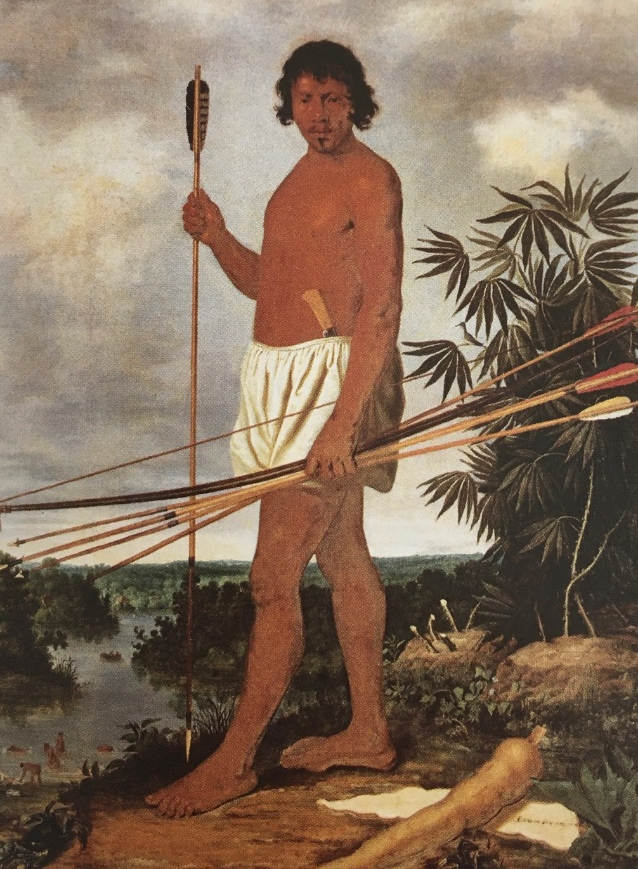
\includegraphics[width=50mm]{articles/02-farinha-e-carne-no-s/01-tupinamba.jpg}};
    \node[inner sep=0pt, anchor=south west, text width=60mm, align=left] (subtitle) at ([xshift=7mm]tupinamba.south east)
            {\small \textsf{\textit{Tupinambá/Homem Brasilian} e detalhe da mandioca. Albert Eckhout. Óleo sobre tela, 272x163 cm. 1643.}};
    \node[inner sep=0pt, anchor=south west] (detail) at ([yshift=5mm]subtitle.north west)
        {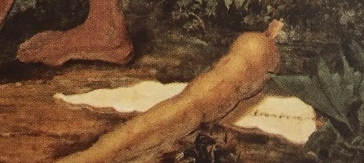
\includegraphics[width=60mm]{articles/02-farinha-e-carne-no-s/02-tupinamba-detalhe.jpg}};
\end{tikzpicture}


\vfill


\begin{tikzpicture}
    \node[inner sep=0pt] (plants) at (0, 0)
        {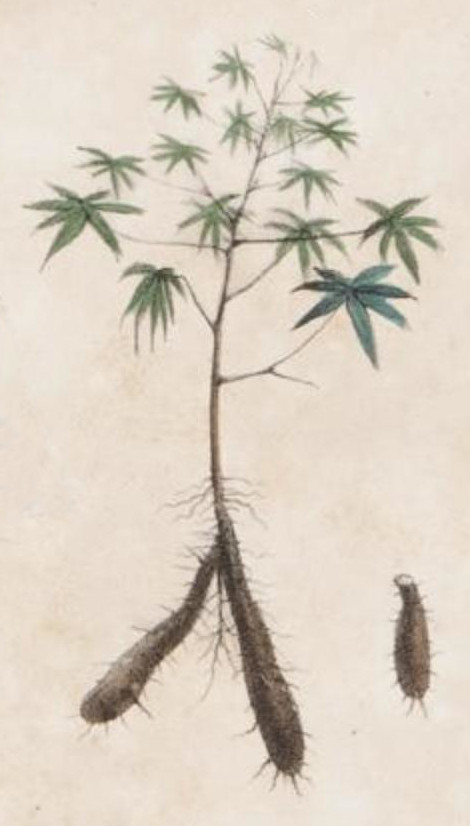
\includegraphics[width=50mm]{articles/02-farinha-e-carne-no-s/04-plantes-nutritives.jpg}};
    \node[inner sep=0pt, anchor=north west, text width=50mm, align=left]
    (subtitleone) at ([yshift=-5mm]plants.south west)
        {\small \textsf{Detalhe de \textit{Plantes Nutritivies} de Jean-Baptiste Debret. Litografia em cores, 51,4x33,4 cm. 1835.}};

    \node[inner sep=0pt, anchor=north west] (study) at ([xshift=21mm]plants.north east)
        {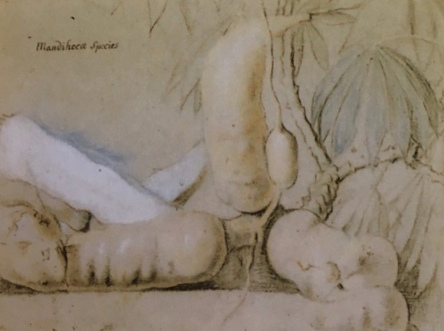
\includegraphics[width=45.4mm]{articles/02-farinha-e-carne-no-s/03-estudo-preparatorio-mandioca.jpg}};
    \node[inner sep=0pt, anchor=south west] (deadnature) at ([xshift=21mm]plants.south east)
        {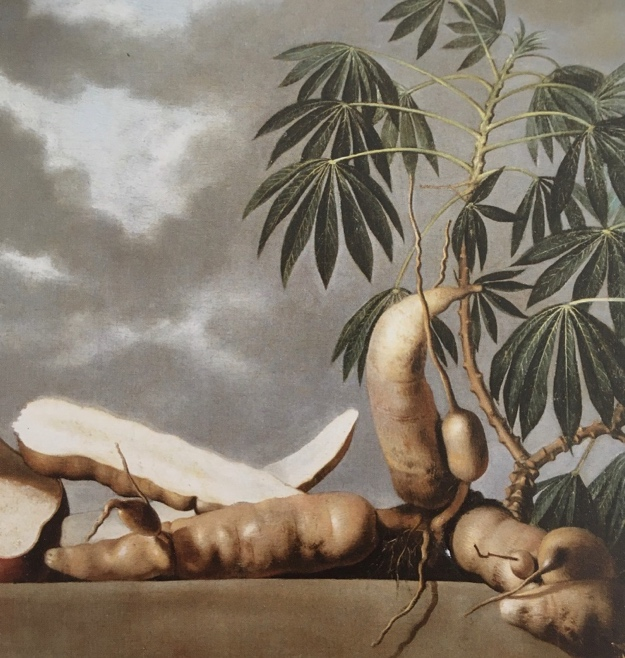
\includegraphics[width=45.4mm]{articles/02-farinha-e-carne-no-s/05-natureza-morta-mandioca.jpg}};
    \node[inner sep=0pt, anchor=north west, text width=47mm] (subtitletwo) at ([yshift=-5mm]deadnature.south west)
        {\small \textsf{\textit{Estudo preparatório} e \textit{Na\-tu\-re\-za-morta com man\-di\-o\-ca} de Albert Eckhout. Óleo sobre tela, 93x90 cm. 1640.}};
\end{tikzpicture}

\end{center}

\clearpage

\hspace*{-10mm}
\begin{tikzpicture}[every node/.style={inner sep=0,outer sep=0}]
    \node[] (engenho) at (0, 0)
        {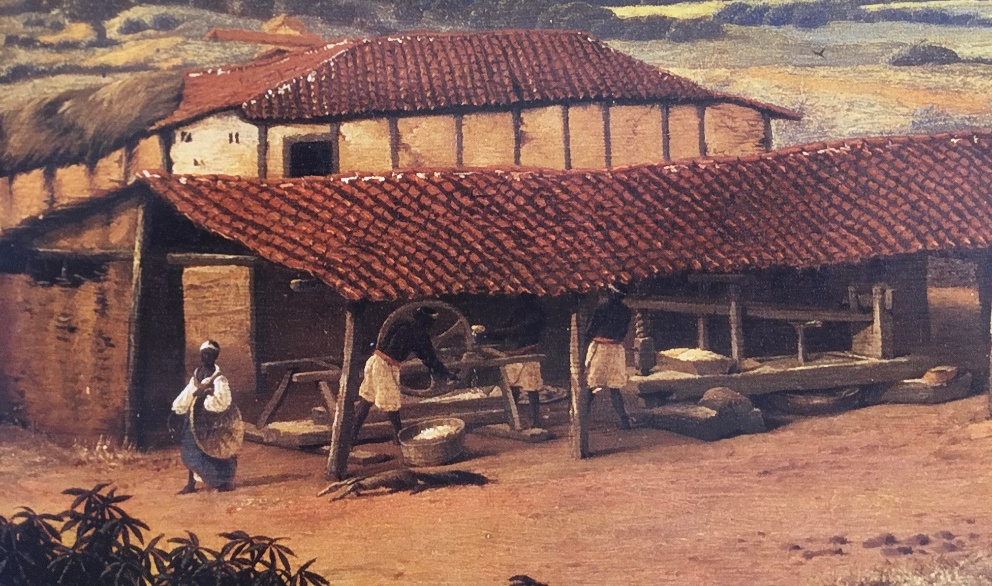
\includegraphics[width=97mm]{articles/02-farinha-e-carne-no-s/06-engenho-mandioca.jpg}};
    \node[anchor=east, text width=34mm, align=right] (caption) at ([xshift=-7mm]engenho.west)
        {\small \textsf{Detalhe de \textit{Engenho de mandioca} de Frans Post. Óleo sobre tela, 47x68 cm. 1651. Coleção particular, Inglaterra.}};
\end{tikzpicture}

\vfill

\hspace*{-16mm}
\begin{tikzpicture}[every node/.style={inner sep=0,outer sep=0}]
    \node[] (preparacao) at (0, 0)
        {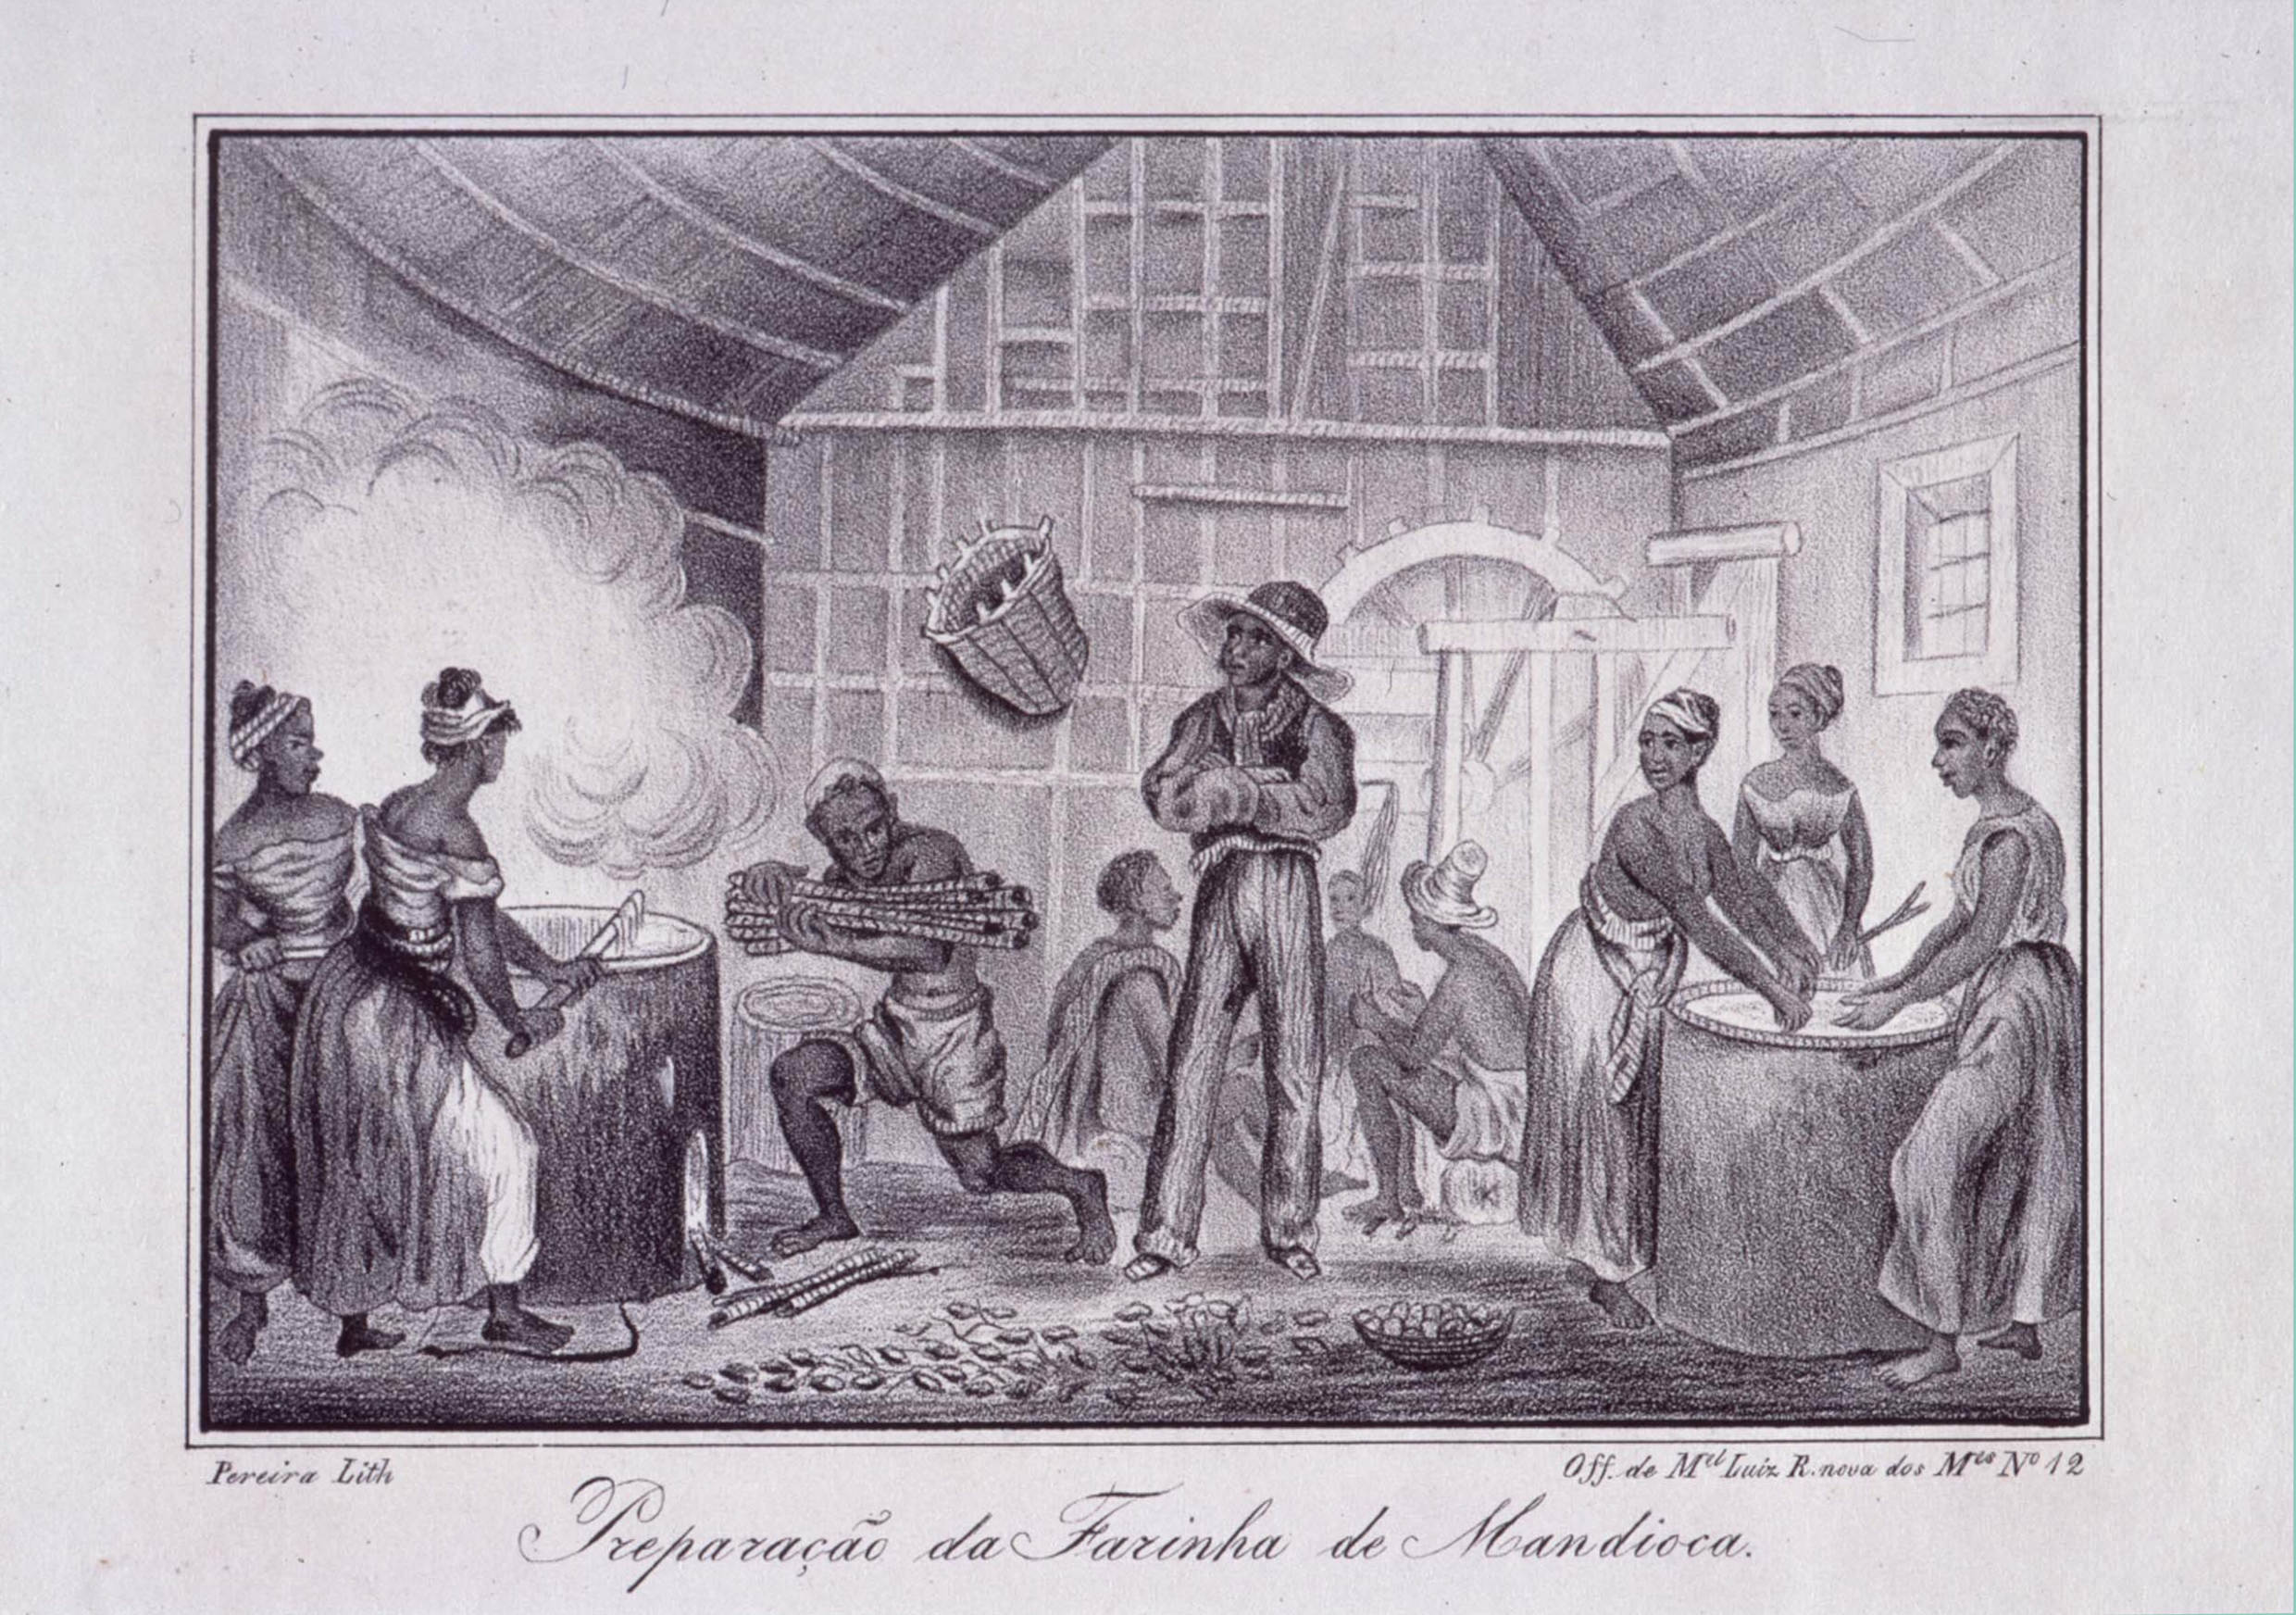
\includegraphics[width=103mm]{articles/02-farinha-e-carne-no-s/07-preparacao-farinha.jpg}};
    \node[anchor=west, text width=34mm] (caption) at ([xshift=7mm]preparacao.east)
        {\small \textsf{\textit{Preparação da farinha de mandioca} de Pereira. Litografia sobre papel, 13,9x18,5 cm. Século XIX. Arquivo Histórico Ultramarino.}};
\end{tikzpicture}

\vfill

\hspace*{-9mm}
\begin{tikzpicture}[every node/.style={inner sep=0,outer sep=0}]
    \node[] (eplucheuses) at (0, 0)
        {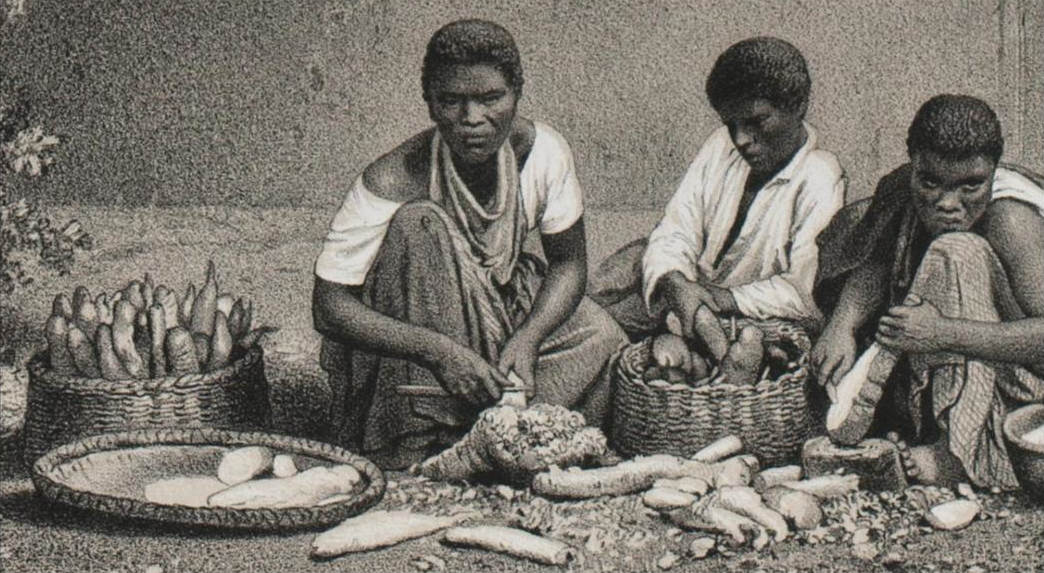
\includegraphics[width=96mm]{articles/02-farinha-e-carne-no-s/08-epluchiuses-mandioca.jpg}};
    \node[anchor=east, text width=34mm, align=right] (caption) at ([xshift=-7mm]eplucheuses.west)
        {\small \textsf{Detalhe de \textit{Éplucheuses de mandioca} de Victor Frond. Litografia sobre papel, 48x63,5 cm. 1861. Coleção particular, Inglaterra.}};
\end{tikzpicture}

\clearpage

\hspace*{-7.5mm}
\begin{tikzpicture}[every node/.style={inner sep=0pt,outer sep=0pt}]
    \node[] (tubinamba) at (0,0)
        {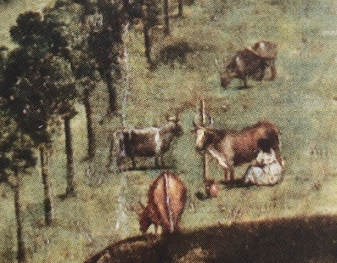
\includegraphics[width=73.5mm]{articles/02-farinha-e-carne-no-s/09-tupinamba-mulher-brazilian.jpg}};
    \node[anchor=west, text width=34mm] (caption) at ([xshift=7mm]tubinamba.east)
        {\small \textsf{Detalhe de \textit{Tupinambá/Mulher Brasilian} de Albert Eckhout. Óleo sobre tela, 274x163 cm. 1643.}};
\end{tikzpicture}

\vfill

\hspace*{5mm}
\begin{tikzpicture}[every node/.style={inner sep=0pt,outer sep=0pt}]
    \node[] (deux) at (0, 0)
        {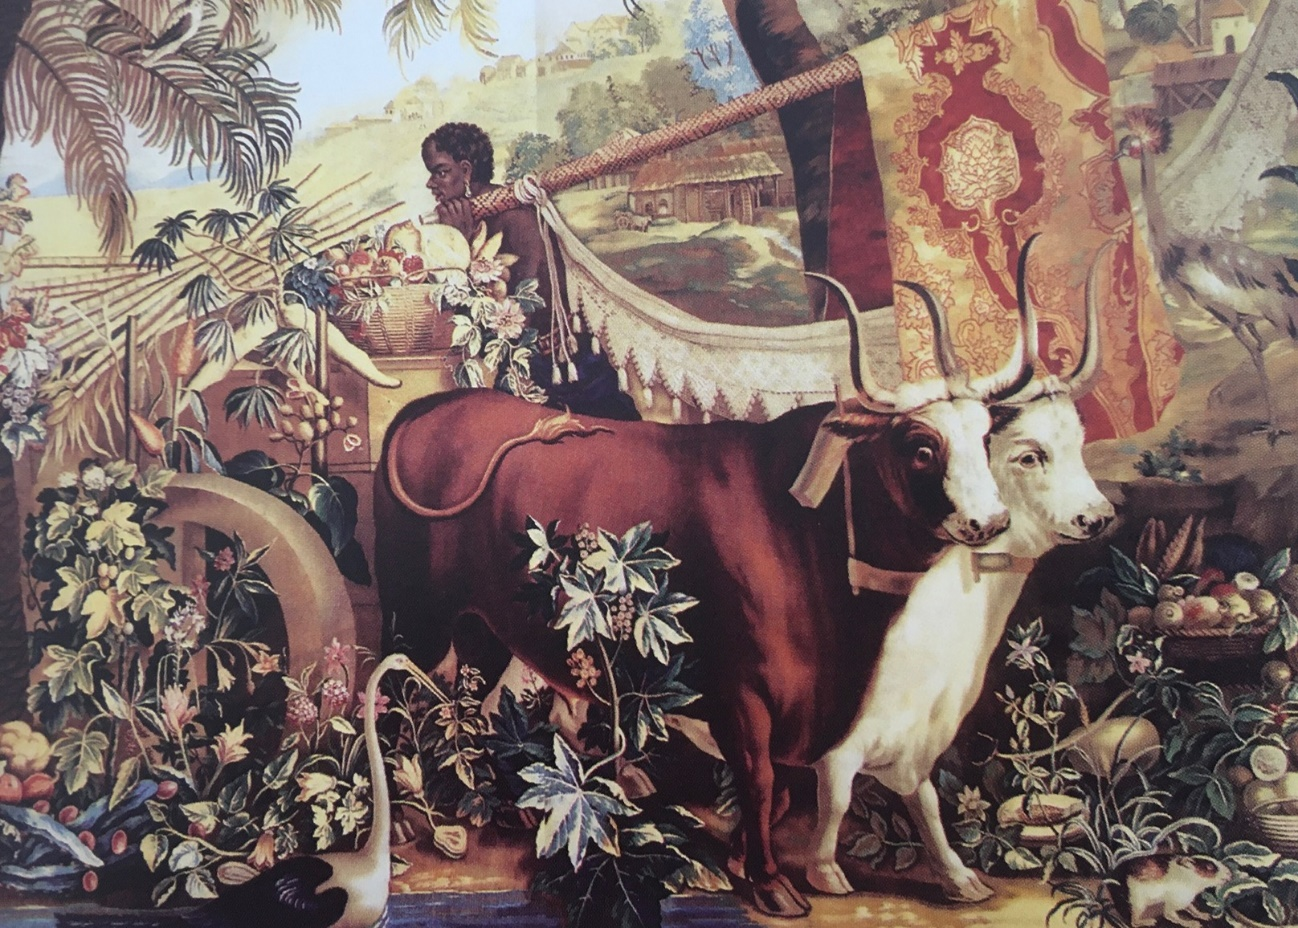
\includegraphics[width=82mm]{articles/02-farinha-e-carne-no-s/10-les-deux-taureaux.jpg}};
    \node[anchor=east, text width=34mm, align=right] (caption) at ([xshift=-7mm]deux.west)
        {\small \textsf{Detalhe de Tapeçaria a partir da obra de Albert Eckhout \textit{“Les deux taureaux”}. Lã e seda, 470x740 cm. Circa de 1690. Mobilier National de France.}};
\end{tikzpicture}

\vfill

\hspace*{-7.5mm}
\begin{tikzpicture}[every node/.style={inner sep=0pt,outer sep=0pt}]
    \node[] (transport) at (0, 0)
        {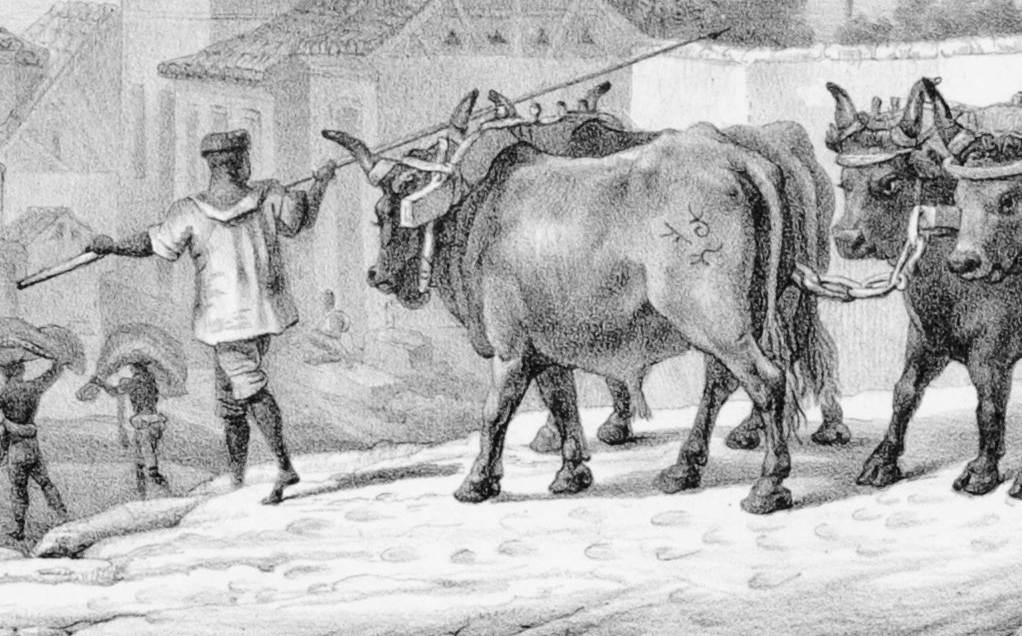
\includegraphics[width=85mm]{articles/02-farinha-e-carne-no-s/11-transport-des-viandes.jpg}};
    \node[anchor=west, text width=34mm] (caption) at ([xshift=7mm]transport.east)
        {\small \textsf{Detalhe de \textit{Transport de viande de boucherie} com marcas de propriedade no gado, de Jean-Baptiste Debret. Litografia em pb, 24,5x25,0 cm. 1835.}};
\end{tikzpicture}

\clearpage

\begin{vplace}
    \centering
    \begin{tikzpicture}
        \node[] (tratado) at (0, 0)
            {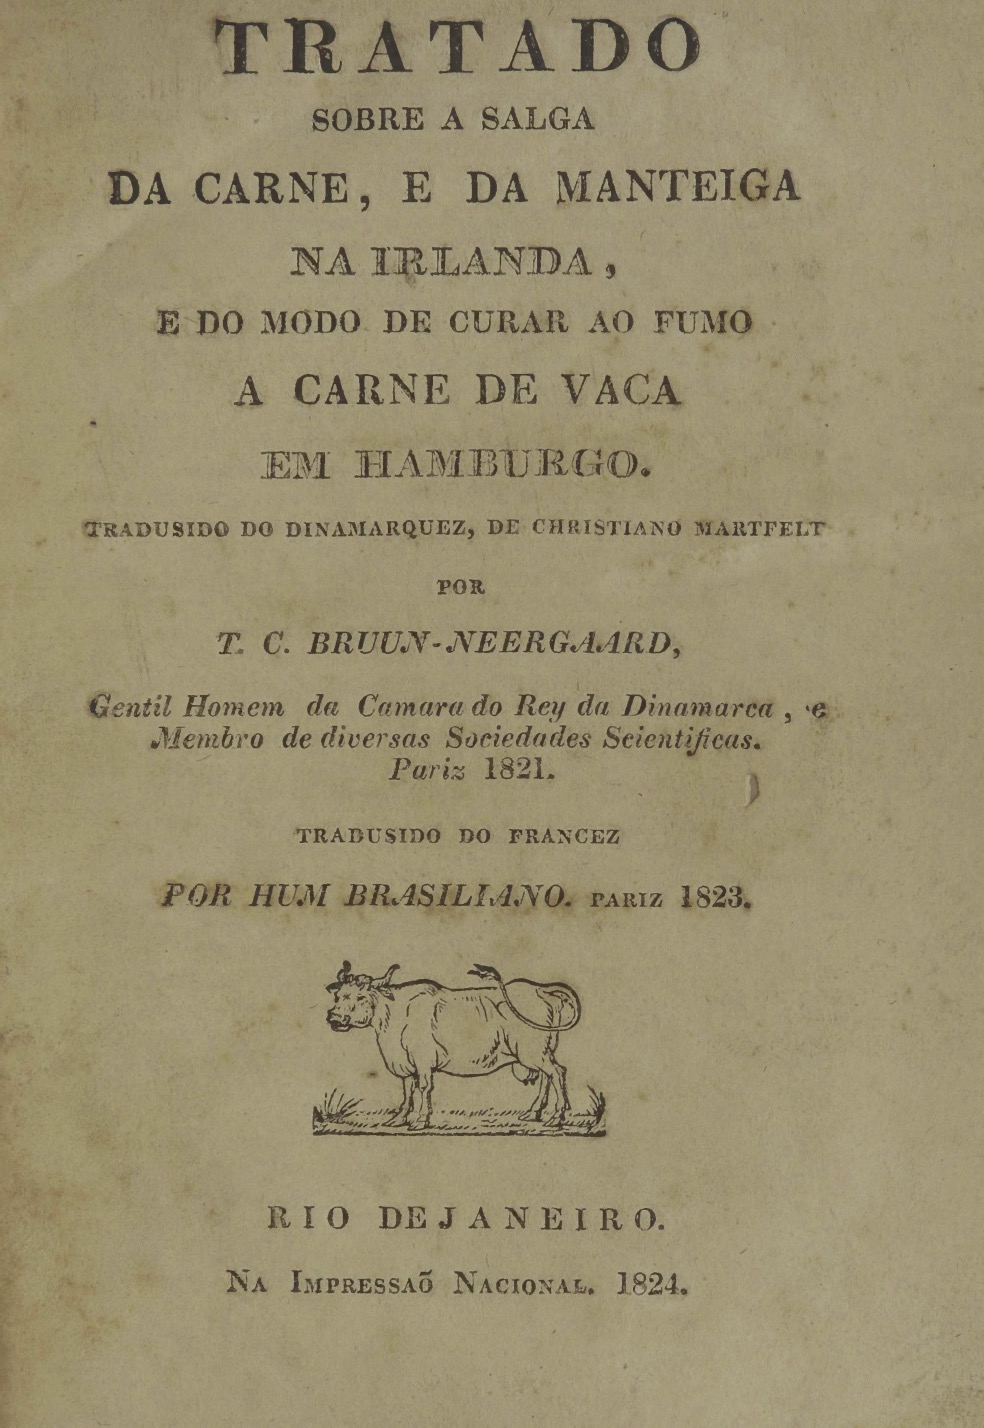
\includegraphics[width=93mm]{articles/02-farinha-e-carne-no-s/12-tratado-sobre-salga.jpg}};
        \node[anchor=north west, text width=93mm] (caption) at ([yshift=-5mm]tratado.south west)
            {\small \textsf{Capa do \textit{Tratado sobre a salga da carne\dots} de Christian Martfelt, traduzido do francês por um brasileiro e impresso no Rio de Janeiro em 1824.}};
    \end{tikzpicture}
\end{vplace}

\clearpage

\begin{vplace}
    \centering

    \begin{tikzpicture}[every node/.style={inner sep=0pt,outer sep=0pt}]
        \node[] (cozinheiro) at (0, 0)
            {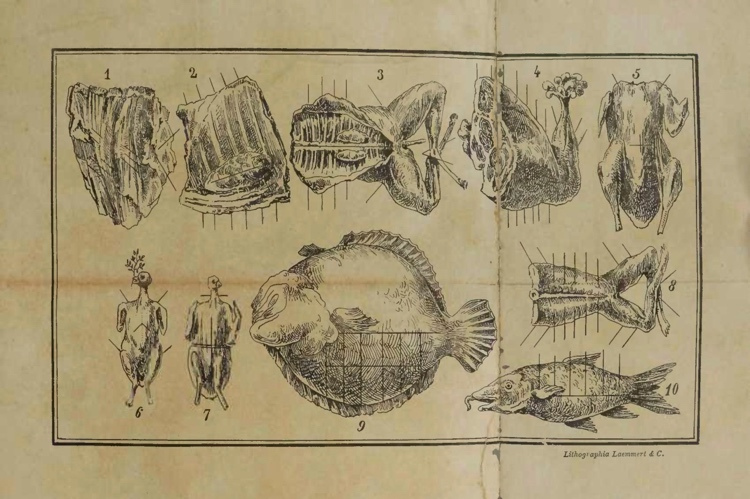
\includegraphics[width=72mm]{articles/02-farinha-e-carne-no-s/13-cozinheiro-imperial.jpg}};
        \node[anchor=south west] (detail) at ([xshift=7mm]cozinheiro.south east)
            {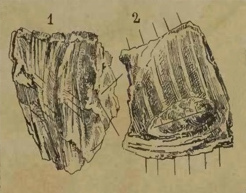
\includegraphics[width=43mm]{articles/02-farinha-e-carne-no-s/14-cozinheiro-imperial-detalhe.jpg}};
        \node[anchor=north west, text width=122mm] (caption) at ([yshift=-5mm]cozinheiro.south west)
            {\small \textsf{Detalhe do apenso da 10ª edição da obra \textit{Cozinheiro Imperial} (1ª ed. 1840) de 1887 mostrando os cortes de carne bovina de R. C. M e impresso no Rio de Janeiro em 1887.}};
    \end{tikzpicture}

    \vspace*{15mm}

    \begin{tikzpicture}[every node/.style={inner sep=0pt,outer sep=0pt}]
        \node[] (boutique) at (0,0)
            {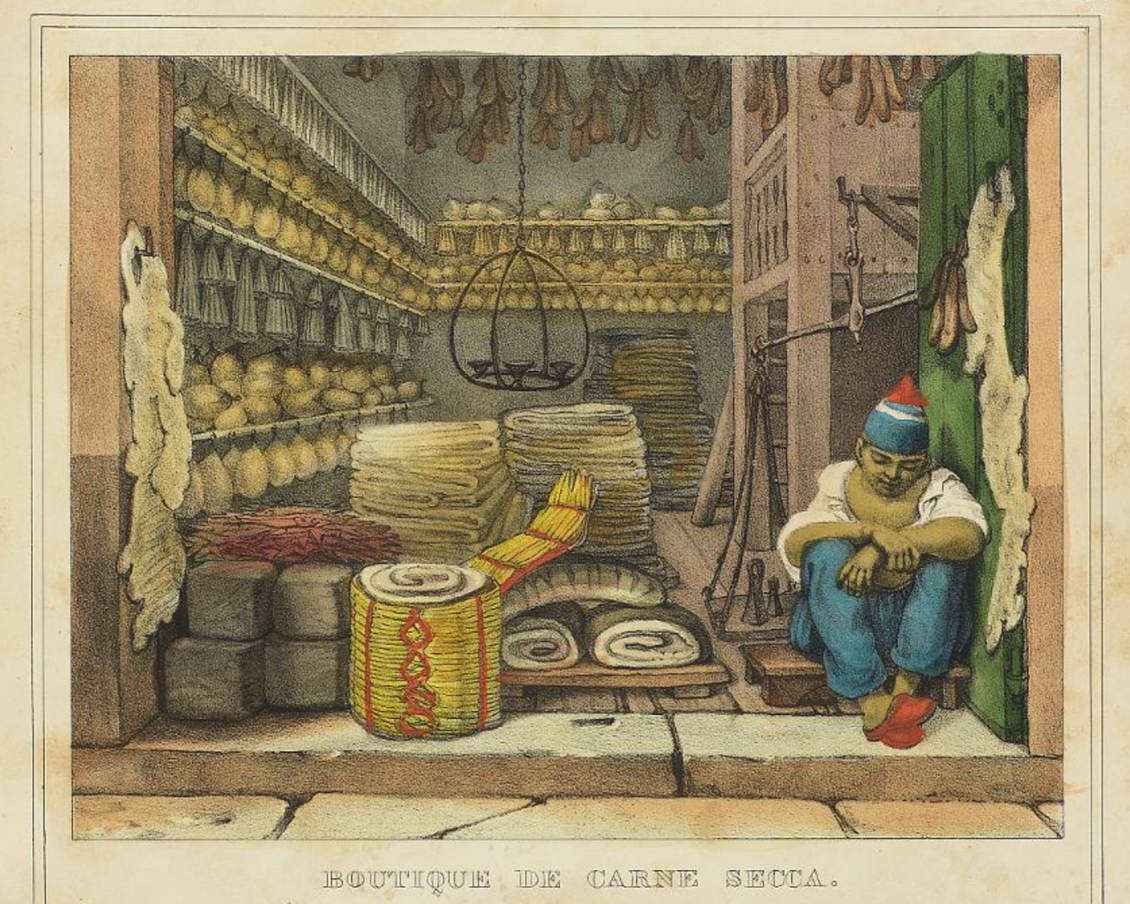
\includegraphics[width=96mm]{articles/02-farinha-e-carne-no-s/15-boutique-de-carne-secca.jpg}};
        \node[anchor=north, text width=82mm] (caption) at ([yshift=-5mm]boutique.south)
            {\small \textsf{\textit{Boutique de carne secca} de Jean-Baptiste Debret. Litografia em cores, 25,8x19,8 cm. 1835.}};
    \end{tikzpicture}

\end{vplace}

\clearpage

\begin{vplace}
    \centering

    \begin{tikzpicture}[every node/.style={inner sep=0pt,outer sep=0pt}]
        \node[] (a) at (0,0)
            {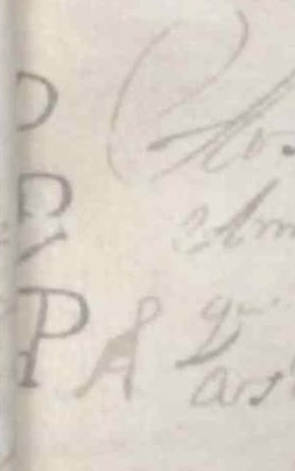
\includegraphics[width=31mm]{articles/02-farinha-e-carne-no-s/16-ferro-de-gado.jpg}};
        \node[anchor=south west] (b) at ([xshift=6mm]a.south east)
            {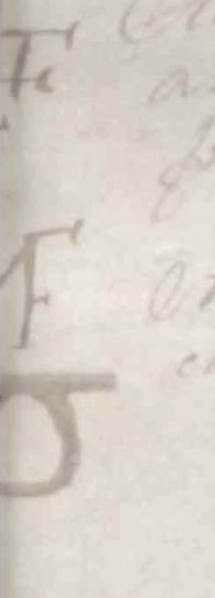
\includegraphics[width=21mm]{articles/02-farinha-e-carne-no-s/17-ferro-de-gado-2.jpg}};
        \node[anchor=south west] (c) at ([xshift=6mm]b.south east)
            {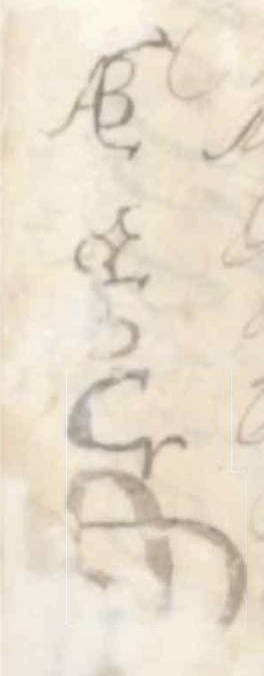
\includegraphics[width=27mm]{articles/02-farinha-e-carne-no-s/18-ferro-de-gado-3.jpg}};
        \node[anchor=south west] (d) at ([xshift=6mm]c.south east)
            {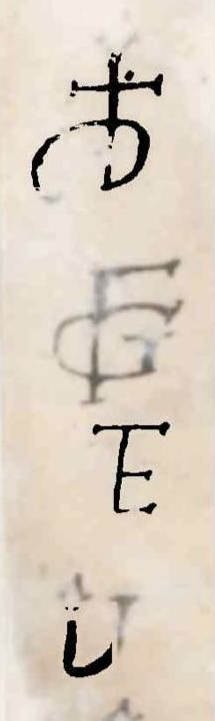
\includegraphics[width=24.5mm]{articles/02-farinha-e-carne-no-s/19-ferro-de-gado-4.jpg}};
        
        \node[anchor=north west, text width=121.5mm] (caption) at ([yshift=-5mm]a.south west)
            {\small \textsf{\textit{Diversos registros de ferro do gado da Capitania do Rio Grande do Norte realizados na Câmara de Natal entre 1673 a 1690} constante no Livro de Registros de Cartas e Provisões da Câmara de Natal de 1673 a 1690.}};
    \end{tikzpicture}

    \vspace*{15mm}

    \begin{tikzpicture}[every node/.style={inner sep=0pt,outer sep=0pt}]
        \node[] (ferrosargento) at (0, 0)
            {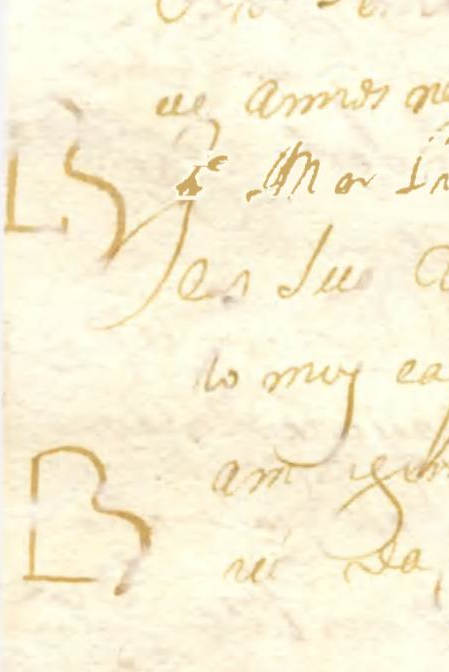
\includegraphics[width=46mm]{articles/02-farinha-e-carne-no-s/20-ferro-de-gado-sgto-mor-leo.jpg}};
        \node[anchor=west, text width=34mm] (caption) at ([xshift=7mm]ferrosargento.east)
            {\small \textsf{\textit{Registro de ferro do gado do Sargento-mor Leonardo Bezerra Cavalcante na Câmara de Natal em 6 de agosto de 1699} constante no Livro de Registros de Cartas e Provisões da Câmara de Natal de 1691 a 1702, p. 92v.}};
    \end{tikzpicture}
\end{vplace}

\clearpage

\begin{vplace}

    \hspace*{-7.5mm}
    \begin{tikzpicture}[every node/.style={inner sep=0pt,outer sep=0pt}]
        \node[] (desenhos) at (0, 0)
            {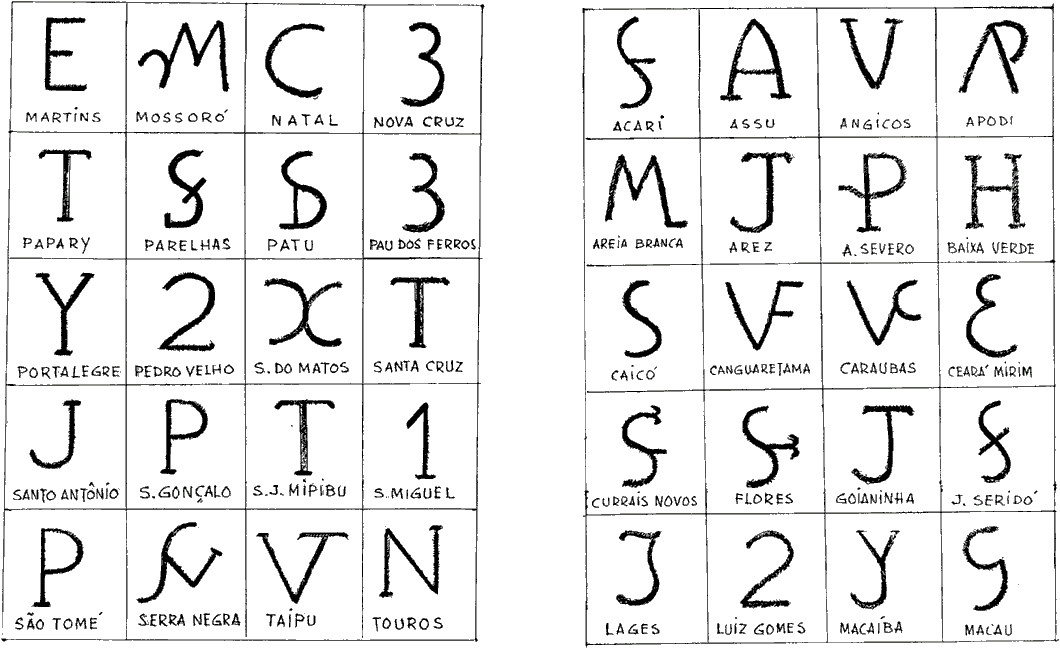
\includegraphics[width=136mm]{articles/02-farinha-e-carne-no-s/22-desenhos-marcas-de-ferro-2.png}};
        \node[anchor=north] at ([yshift=-6mm, xshift=2mm]desenhos.south)
            {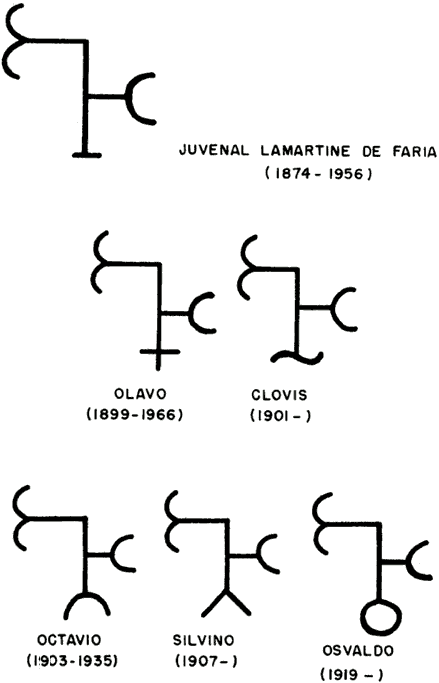
\includegraphics[width=56mm]{articles/02-farinha-e-carne-no-s/21-desenhos-marcas-de-ferro.png}};
        \node[anchor=south, text width=\textwidth] (caption) at ([yshift=5mm]desenhos.north)
            {\small \textsf{\textit{Desenhos utilizados nas marcas de ferro para gado do Rio Grande do Norte, séc. XIX--XX} por Oswaldo Lamartine de Faria em sua obra ``Ferro de Ribeiras do Rio Grande do Norte'' de 1984.}};
    \end{tikzpicture}
\end{vplace}

\label{chap:farinhaend}

\end{refsection}

\begin{refsection}
\renewcommand{\thefigure}{\arabic{figure}}

\chapterTwoLines
{Não ao peso, não ao recrutamento}
{os Quebra-quilos e as autoridades públicas no Rio Grande do Norte (1874--1875)}
\label{chap:naoaopeso}

\articleAuthor
{João Fernando Barreto de Brito}
{Doutor pelo Programa de Pós-Graduação em História Social da Universidade Federal do Rio de Janeiro (PPGHIS/UFRJ). ID Lattes: 2836.1238.5025.4834. ORCID: 0000-0003-1692-8703. E-mail: joaofernandohistoria@gmail.com.}

\begin{galoResumo}
    \marginpar{
        \begin{flushleft}
        \tiny \sffamily
        Como referenciar?\\\fullcite{SelfBrito2021}\mybibexclude{SelfBrito2021}, p. \pageref{chap:naoaopeso}--\pageref{chap:naoaopesoend}, \journalPubDate{}
        \end{flushleft}
    }
    No ano de 1874 as notícias sobre as ações dos Quebra-quilos circulavam com grande velocidade na província do Rio Grande do Norte. As feiras, casas comerciais e tabernas eram espaços privilegiados para a disseminação das fofocas e mexericos em torno de uma onda de revoltas nascidas no interior da Paraíba do Norte. A cada momento, notícias chegavam aos ouvidos de autoridades públicas, mas também de pessoas que se mostraram insatisfeitas com a política imperial, com os impostos municipais, com o recrutamento por sorteio e, sobretudo, com a lei que estabeleceu oficialmente o Sistema Métrico Decimal Francês (SMD), substituindo as tradicionais costumeiras medidas antropométricas lusitanas, prevendo multa e prisão para aqueles que ousassem desrespeitar tal determinação. O presente artigo investigou a atuação dos Quebra-quilos no Rio Grande do Norte, destacando vilas e povoações atingidas por esses sediciosos, identificando os grupos sociais partícipes, suas estratégias, e a maneira pela qual as autoridades públicas e militares combateram os revoltosos na citada província. Problematizamos fontes oficiais, correspondências, códices, periódicos de época e ofícios do governo Imperial. 
\end{galoResumo}

\galoPalavrasChave{Quebra-quilos. Sistema métrico decimal. Rio Grande do Norte.}

\begin{otherlanguage}{english}

\fakeChapterTwoLines
{No to weight, no to recruitment} {The Quebra-quilos rebels and public authorities in Rio Grande do Norte (1874--1875)}

\begin{galoResumo}[Abstract]
    In the year 1874, news about the actions of Quebra-Quilos rebels spread out quickly in the province of Rio Grande do Norte. Street markets, commercial houses and taverns were privileged spaces for spreading rumors and gossip about a wave of revolts started in the countryside of Paraíba do Norte. At every moment news reached public authorities, but it also echoed in sectors of society who were dissatisfied with imperial policy, municipal taxes, recruitment by drawing lots, and most of all the law that officially established the French Decimal Metric System (SMD), replacing the traditional customary Portuguese anthropometric measures and imposing fine and imprisonment for those who dared to disrespect such determination. The present article investigates the actions of Quebra-quilos in Rio Grande do Norte, highlighting the villages and towns affected by these seditious people, identifying the participating social groups, their strategies, and the way public and military authorities fought the rebels in that province. We problematize official sources, correspondences, codices, press reports of that time and official letters by the Imperial government.
\end{galoResumo}

\galoPalavrasChave[Keywords]{Quebra-quilos. Decimal Metric System. Rio Grande do Norte.}
\end{otherlanguage}

\section{Introdução}

Já nos últimos dias do mês de novembro de 1874, povoações e vilas do interior paraibano e pernambucano foram atacados pelos Quebra-quilos.\footnote{É possível compreender o significado atribuído na época à palavra “quebra-quilos” a partir da visão do Imperador Dom Pedro II, demonstrada em sua “Falla do Throno” diante da assembleia geral em 16 de março de 1875, oportunidade em que ordem pública novamente havia sido perturbarda, desta vez no interior de quatro províncias do Norte, perpetradas por “bandos sediciosos, em geral movidos por fanatismo religioso e preconceitos contra a pratica do systema metrico, assaltaram povoações, e destruiram archivos e padrões dos novos pesos e medidas”. Esta maneira de enxergar os seus súditos descontentes de certo servia como forma de deslegitimar a ação dos revoltosos, de modo que não reconhecia as reclamações e protestos proferidos por tais. Por outro lado, estigmatizava-os como “bandos sediciosos”, fazendo-se alusão a grupos de salteadores, estes impulsionados pela ignorância, por não aceitarem o sistema métrico imposto pelo governo, tresloucados religiosos, ou seja, que não agiam motivados pela razão. Ver SENADO FEDERAL. \textbf{Biblioteca Digital}. Falla do Throno na abertura da assembléa geral de 16 de março de 1875. Disponível em: <http://www2.senado.leg.br/bdsf/item/id/227319>, acessado em 29 de julho de 2016.} Feiras locais, casas comerciais, paróquias, coletorias e até as residências de pessoas influentes dessas localidades (juízes, coletores de rendas, subdelegados e delegados) foram alvos desses revoltosos. A situação entre os do \textit{mundo do governo} era de preocupação. Na província do Rio Grande do Norte adotaram-se medidas “preventivas”, prepararam-se com a finalidade de conter os agitadores. Oito dias após as primeiras agitações verificadas na província de Pernambuco, o Rio Grande do Norte recebeu da Secretaria dos Negócios de Guerra uma considerável quantidade de armamento. Parecia que os representantes provinciais sabiam da inevitabilidade dos conflitos e \textit{armaram-se até os dentes}, como diz o ditado popular. 

Mais de 22 mil utensílios a serem usados em combates desembarcaram em Natal, de onde seriam distribuídos para aqueles responsáveis por evitar o furor dos Quebra-quilos. O envio de espingardas raiadas, cartuchos, cápsulas, bornais entre outros objetos é de fato resultado do conhecimento prévio das autoridades acerca da proximidade dos confrontos com os Quebra-quilos.\footnote{Arquivo Nacional, Brasil --- Código NP, Fundo ``Diversos códices da antiga SDH''. Notação do documento “Códice 603 v. 5”. Dr. José Maria Lopes da Costa, Secretaria do Estado dos Negócios de Guerra, em 29 de novembro de 1874, p.~24.}

Outra medida de prevenção articulada pelas autoridades do Rio Grande do Norte foi tomada ainda em 4 de dezembro de 1874, conforme publicou o jornal D. Pedro II, quando “partio o chefe de polícia Dr. Luiz Ignacio Barreto com destino á comarca de S. José e a diversos pontos da de Canguaretama, limitrophes da província da Parahyba, no intuito de providenciar em ordem a prevenir a invasão dos insurgentes daquella província”.\footnote{Biblioteca Nacional, Brasil (Hemeroteca Digital) --- D. Pedro II, n. 34, 24 de dezembro de 1874, p.~2.}

Um dia depois, Bandeira de Mello ainda demonstrava preocupação em relação a proteção da província, de modo que solicitou ao presidente pernambucano Henrique Pereira de Lucena, em virtude da “falta de armamento no Deposito de artigos belicos d’esta Província”,\footnote{Arquivo Público do Estado de Pernambuco Jordão Emerenciano [APEJE] --- Coleção correspondências entre presidentes de província, PP 53,1874, p. 290.} mais armamentos tendo em vista às “occurrencias que se vão dando na Província da Parahyba e de que se acham ameaçadas alguns pontos desta”.\footnote{Ibidem.} Naquele mesmo mês, em dia de 5 de dezembro de 1874, as previsões se confirmaram e aos poucos vários lugares seriam também palco das ações dos Quebra-quilos, como podemos observar da figura \ref{fig:quebra-quilo-rn}. 

\begin{figure}[ht]%
    \centering%
    \caption{Quebra-quilos no Rio Grande do Norte}%
    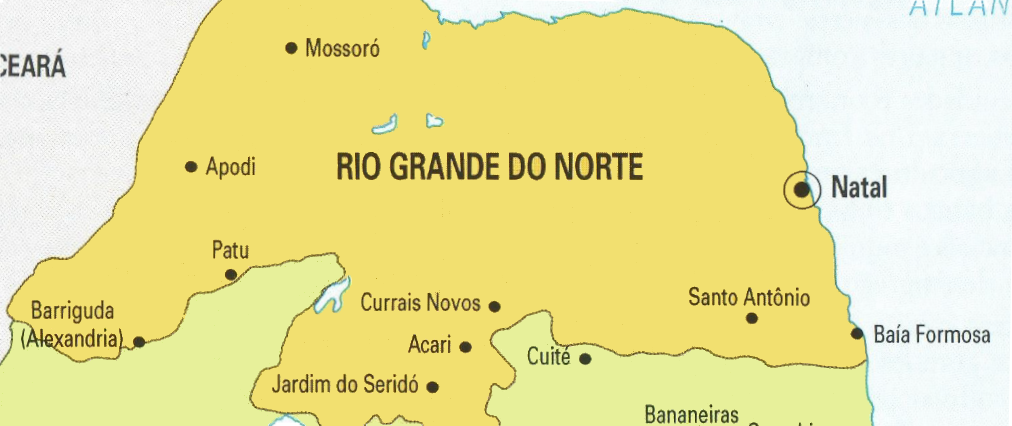
\includegraphics[width=.75\textwidth]{articles/03-nao-ao-peso-nao-ao-r/01-rn.png}%
    \caption*{Fonte: \textcite[p.~17]{Monteiro1993}}%
    \label{fig:quebra-quilo-rn}%
\end{figure}%

O presente artigo visa investigar a atuação dos Quebra-quilos no Rio Grande do Norte. Destacaremos as vilas e povoações atacadas por esses sediciosos, que grupos sociais participaram ativamente, quais estratégias foram utilizadas por eles, e como as autoridades públicas e policiais norte-rio-grandenses lidaram com esta que foi a maior revolta popular do século XIX. Serão investigadas fontes oficiais do governo, tais como correspondências entre presidentes de províncias, o códice 603 (fonte que reuniu vários documentos ministeriais da Guerra e da Justiça sobre a revolta), além de diversos periódicos. Analisaremos os discursos e falas das autoridades, bem como problematizaremos as ações, experiências e estratégias dos Quebra-quilos.

\section{Desenvolvimento}

Segundo a folha noticiosa \textbf{Diário de Pernambuco}, insurgentes da Paraíba transpassaram os limites provinciais e adentraram o Rio Grande do Norte em 5 dezembro de 1874. De acordo com o referido jornal, cerca 200 indivíduos denominados “quebra-kilos”, que unidos a mais 100 pessoas do lugar invadiram a feira da povoação de Santo Antônio, município de Goianinha, causando a destruição de pesos e medidas do SMD em diferentes estabelecimentos. Destacava a mencionada folha noticiosa, pretendiam os sediciosos adentrar a casa do padre capelão com o intuito de queimarem os livros de batismo dos filhos livres de mulheres escravas, algo não realizado posto que foram demovidos de suas intenções pelo subdelegado local.\footnote{Biblioteca Nacional, Brasil (Hemeroteca Digital) --- Diário de Pernambuco, ed. 286, 15 de dezembro de 1874, p.~1.}

Ao atacarem a povoação de Santo Antônio (RN), os sediciosos usaram de estratégias já bem conhecidas, repetindo-se o \textit{modus operandi} das ações tidas nas províncias da Paraíba e Pernambuco. Parece-nos que a experiência dos ataques passados ainda na região da Borborema norteou as investidas tanto do lado pernambucano quanto do lado rio-grandense. A feira se manteve como espaço de aglutinação de novos revoltosos (dos paraibanos com os nativos) e o lugar de demonstrar as insatisfações com as políticas e autoridades imperiais. Isto porque a escolha de um alvo limítrofe à Paraíba não era algo aleatório. Os insurgentes paraibanos “invadiram” Santo Antônio e somaram-se a mais indivíduos deste povoado.

É preciso trazer à tona também a participação ativa de sujeitos pardos, caboclos e negros (escravos(as), ex-escravos(as) e gente livre) em algumas ações ocorridas no Rio Grande do Norte. Atentos às transformações promovidas pela lei do Ventre Livre (1871), cuja obrigatoriedade de comprovação da propriedade escrava passava a ser de responsabilidade do proprietário e não mais do cativo, e para a condição que envolvia a condição do escravo ingênuo a depender de sua data de nascimento, podemos inferir que a procura de certos sediciosos pelos livros de batismos de filhos livres de mulher escrava era um meio de evitar com que estes se tornassem escravos ilegalmente. Evitava-se que o senhor de falsificasse a data do registro de nascimento daqueles e/ou impossibilitava a comprovação da propriedade por este.\footnote{A presença de pessoas negras nas revoltas do Quebra-quilos no Rio Grande do Norte pode se averiguar a partir da ação que intencionava a queima da documentação cartorial, que para além de se querer evitar o pagamento de impostos ou dívidas também envolviam os documentos de matrículas de escravos, classificação de escravos e o registro de nascimento e óbito dos ingênuos, o que colocava em dificuldades a comprovação da propriedade escrava pelo senhor, portanto o que nos leva a crer que a participação de negros cativos nestas revoltas é um elemento pertinente. Lembremos que o historiador Luciano Mendonça já chamava a atenção para os casos de participação de escravos, ex-escravos e gente negra nas sedições em Campina Grande. No Rio Grande do Norte os estudos sobre a história dos negros e de suas lutas ainda são poucos, podemos citar alguns trabalhos como os de \fullcite{Mattos1985}; \fullcite{Assuncao1994}; \fullcite{Borges2000}; \fullcite{Macedo2005}; \fullcite{Macedo2015}; \fullcite{Lopes2011}; \fullcite{Pereira2014}.}

Ademais, o desfecho desta passagem dos sediciosos por Santo Antônio teve início quando uma força policial, composto de 53 praças de linha e guiada pelo alferes João Ferreira Oliveira, foi destacada para o termo de Canguaretama, sede da comarca. O coronel Bonifácio Francisco Pinheiro da Câmara (que foi o segundo vice-presidente do Rio Grande do Norte em 1873, além de chefe do partido Conservador da mesma província), naquele momento comandante superior da Guarda Nacional, articulou no mesmo dia um contingente da capital para enviar ao local. Isto teria desmobilizado os sediciosos que recuaram em suas intenções, mas não por muito tempo.\footnote{Biblioteca Nacional, Brasil (Hemeroteca Digital) --- Diário de Pernambuco, ed. 286, 15 de dezembro de 1874, p. 1.}

Bandeira de Mello e Filho comunicou em carta endereçada ao presidente Henrique Pereira de Lucena no dia 7 de setembro de 1874, que no município de São José de Mipibú, 40 quilômetros de Canguaretama, “desordeiros” da povoação de Santa Rita da Cachoeira se manifestaram contra os pesos e medidas. Repetia-se a fórmula anterior até que um boato sobre alguns sujeitos que acusados de serem “republicanos e defensores das liberdades públicas”\footnote{Ibidem} se preparavam para organizar um motim na feira daquele lugar, de modo a fazer com que o povo acompanhasse “o movimento sedicioso apurado na Província visinha [Paraíba]”\footnote{Não sabemos a procedência ou a veracidade desse boato, porém é estranho ao movimento Quebra-quilos no geral que bandeiras e ideias republicanas fossem levantadas como forma de reivindicação. Esta pode ter sido uma forma do presidente do Rio Grande do Norte alegar a Lucena a urgência das ajudas que solicitou ao mesmo ou se foi algo peculiar daquele episódio. Não há registros iguais a este nem relatos parecidos. Os protestos dos Quebra-quilos não pretendiam sucumbir a ordem imperial vigente, aliás se caracterizava por um movimento composto inclusive por gente do governo e por ser anti-fiscal. Isto nos leva a crer que tal “boato”, portanto, não passou de uma artimanha do senhor Bandeira de Mello.}.

O \textbf{Diário do Rio de Janeiro} não demorou a trazer novas notícias “desagradáveis” da província do Rio Grande do Norte. Segundo o jornal em 14 de dezembro na cidade de Goianinha, cerca de 300 homens entraram na casa de câmara e cadeia e quebraram pesos e medidas. Além disso, tentou-se queimar os arquivos públicos, entretanto foram impedidos por alguns policiais e pessoas que o periódico classificou como “respeitáveis do logar”\footnote{Biblioteca Nacional, Brasil (Hemeroteca Digital) --- Diário do Rio de Janeiro, ed. 347, 16 de dezembro de 1874, p. 1.}, o que indica o grau de influência e talvez econômico destas.

As notícias reproduzidas pelos jornais de que “a maior parte dos sediciosos eram sertanejos, desertores, criminosos e sentenciados”\footnote{Ibidem, p.~1.} não são dignas de total confiança, uma vez que estes estereótipos recaíam com grande frequência sob a \textit{arraia miúda} e multiplicavam preconceitos. Ora, já (d)enunciamos a participação de pessoas de cabedal ligadas a esse movimento\footnote{Ver ``Gráfico 1'' em \fullcite[p.~171]{Brito2020}.}.

O jornal \textbf{D. Pedro II}, da cidade de Fortaleza, em 24 de dezembro reproduziu do jornal \textbf{O conservador} (RN) as notícias das agitações ocorridas no início de dezembro de 1874 na província norte-rio-grandense. Na terceira página acabou por reportar o discurso de que “a população de toda a província mostra-se infensa aos invasores, e disposta a apoiar a acção da autoridade”\footnote{Biblioteca Nacional, Brasil (Hemeroteca Digital) --- D. Pedro II, n. 34, 24 de dezembro de 1874, p. 2--3.}, o que na realidade não acontecia. Isto porque parte da população continuava a apoiar os paraibanos revoltosos e a engrossar as fileiras sediciosas contra as determinações imperiais. Talvez tal “população” a qual se referia a folha rio-grandense, aliás da situação conservadora, não correspondesse ao todo, mas a uma parte daqueles “respeitáveis do logar”\footnote{Biblioteca Nacional, Brasil (Hemeroteca Digital) --- Diário do Rio de Janeiro, ed. 347, 16 de dezembro de 1874, p. 1.}, apenas uma parcela.  

A povoação de Currais Novos (distante mais de 100 quilômetros da divisa com a Paraíba), na época pertencente ao município de Acari, foi invadida pelos Quebra-quilos que seguiram em marcha para a vila de Sant’Anna do Seridó (hoje município de Santana do Matos), quase 60 quilômetros adiante. Nesta ocasião, o juiz municipal e outras autoridades locais de Sant’Anna reuniram 100 homens a fim de frear o ímpeto dos sediciosos. Segundo o \textbf{Diário de Pernambuco}, até o dia 19 de dezembro nenhum agitador havia arriscado adentrar naquele lugar, de maneira a comemorar a iniciativa das pessoas locais em organizar-se para repelir os revoltosos. Tal exemplo, congratulava ainda a referida folha noticiosa, “é digno de ser imitado e muito honra aos cidadãos que tão espontanea e patrioticamente se empenham em defeza da ordem publica”\footnote{Biblioteca Nacional, Brasil (Hemeroteca Digital) --- Diário de Pernambuco, ed. 04, 6 de janeiro de 1875, p. 3.}.

A demonstração de resistência contra os avessos ao SMD representava a frágil organização policial de cada uma dessas localidades distantes das capitais provinciais. A falta de efetivos e de pessoas qualificadas não eram os únicos problemas do aparato repressor imperial, especialmente nos espaços mais profundos do Norte Agrário retratado por Evaldo Cabral de Melo. Da deficiência estrutural do estado imperial surgiam organizações particulares que se utilizavam da força e da violência, era assim com os Quebra-quilos, era assim com aqueles que \textit{voluntariamente} pegavam em armas para repeli-los.  

Sobre as agitações no Rio Grande do Norte, o jornal \textbf{O Mossoroense} deu destaque ao diferente nome atribuído ao Quebra-quilos, movimento que segundo o jornal chegou à região seridoense\footnote{Seridó é uma macrorregião do Rio Grande do Norte, que compreende atualmente aos municípios de Acari, Carnaúba dos Dantas, Caicó, Cruzeta, Currais Novos, Equador, Ipueira, Jardim de Piranhas, Jardim do Seridó, Ouro Branco, Parelhas, Santana do Seridó, São Fernando, São João do Sabugi, São José do Seridó, Serra Negra do Norte e Timbaúba dos Batistas. Esta região é caracterizada pela vegetação seca e pelo clima semiárido. Ver \cite{Abrantes2011}.} com outra designação. “\textbf{Ronco da abelha} --- He com este nome que já chegou no Seridó desta província a revolução parahybana chamada – Quebra-Killos” [grifo da fonte]\footnote{Museu Histórico Lauro da Escóssia, Mossoró/RN --- O Mossoroense, n. 99, 20 de dezembro de 1874, p.~2.}. A comparação se faz notória sob o prisma da experiência da luta popular, já que ambas as revoltas estiveram relacionadas à insatisfação da população pobre frente às modificações das leis referentes aos registros de nascimento, batismo e óbito e do censo geral --- na ocasião o de 1851, barrado pelo \textit{Ronco} dos revoltosos, e o realizado em 1872, o primeiro do Brasil, apesar de questionáveis e polêmicas sobre sua feitura \cite{Oliveira2005}.

O mesmo periódico enunciou a existência de boatos que diziam respeito a invasão da vila do Acary pelo “Ronco da Abelha” e de Jardim (hoje Jardim de Piranhas, posto que a sua quase homônima Jardim do Seridó se chamava à época apenas “Seridó”). Nesta última os Quebra-quilos festejaram suas ações na feira e inutilizaram pesos e balanças “ao som de música e foguetes”\footnote{Museu Histórico Lauro da Escóssia, Mossoró/RN --- O Mossoroense, n. 99, 20 de dezembro de 1874, p.~2.}, que foi obrigada a tocar para e pelos sediciosos. Longe de representar uma mera atividade lúdica, como nos alertou Maria Clementina Pereira Cunha\footnote{As festas, conforme Cunha, são hoje objeto de estudo da história social da cultura, compreendidas como manifestações, espaços de tensões e conflitos. Segundo a autora, por meio delas o historiador “poderá espiar uma rica miríade de práticas, linguagens e costumes, desvendar disputas em torno de seus limites e legitimidades, ou da atribuição de significados, e sentir as tensões latentes sob as formas lúdicas, [...] captar manifestações de dor, revolta, alegria, presentes nos dias de festa como nos dias comuns”. \cite[p.~12]{Cunha2002}.}, a festa fez-se na expressão do descontentamento coletivo dos sediciosos em relação às políticas imperiais. O som da banda marcial ecoava como vitória aos ouvidos dos Quebra-quilos. Celebrava-se o descumprimento da lei métrica. Resistia-se à disposição imposta de “cima para baixo”. \cite[p.~13]{Cunha2002}.

O \textbf{Diário de Pernambuco}, por sua vez, evidenciou as agitações dos Quebra-quilos em 13 de dezembro de 1874 na povoação de Poço Limpo (pertencente naquele tempo ao município de São Gonçalo, hoje grande Natal), lugar em que os sediciosos atacaram os exemplares do metro, pesos e balanças e as casas dos comerciantes locais. O jornal exemplifica o caso do comerciante português Lourenço José Corrêa, que se negando a entregar pesos e medidas foi espancado pelos revoltosos juntamente com o seu filho.\footnote{Biblioteca Nacional, Brasil (Hemeroteca Digital) --- Diário de Pernambuco, ed.~293, 23 de dezembro de 1874, p.~1.} Não eram raras as ameaças endereçadas às autoridades e comerciantes locais, especialmente àqueles que se mostravam guardiães dos interesses imperiais.  

Poucos quilômetros de São Gonçalo, comerciantes da vila de Macaíba estiveram igualmente sob a ameaça da \textit{turba}. Todavia, há de se destacar que havia uma diferença entre a perseguição aos comerciantes nascidos no Brasil e aqueles provenientes de outras nações, o que se caracterizou em certos casos como ações de xenofobia. Podemos inferir a respeito da existência de preconceitos entre tais comerciantes locais com os de fora, mas também existia a queixa dos brasileiros de que estrangeiros monopolizavam o comércio a retalho, beneficiando-se ao enganarem os pequenos comerciantes, pois manejavam habilmente os preços, açambarcando e especulando, assim como utilizavam os novos padrões métricos, diferentemente dos primeiros. 

Em correspondência de Bandeira de Mello ao presidente pernambucano Pereira de Lucena, datada de 19 de dezembro de 1874, o primeiro comunicava a invasão da vila de Sant’Anna do Mattos por um grupo composto por cerca de 200 indivíduos, que nos dizeres daquela autoridade eram “homens mal intencionados”\footnote{APEJE --- Coleção correspondências entre presidentes de província, PP 53, p. 297.}, cuja ordem obedeciam a um tal de Cipriano Lopes Pequeno. Em Baía Formosa, à época povoação de Canguaretama, no dia 22 de dezembro “sediciosos conhecidos por quebra-kilos praticaram desordens, destruindo pesos e medidas dos poucos estabelecimentos alli existentes”\footnote{Biblioteca Nacional, Brasil (Hemeroteca Digital) --- Diário de Pernambuco, ed. 286, 15 de dezembro de 1874, p.~3.}, conforme noticiou o \textbf{Diário de Pernambuco}. Antônio Jeronymo, o delegado de polícia local, fez frente ao movimento junto a 25 praças de linhas e o alferes Paula Moreira, o que resultou na prisão de dois revoltosos, Manoel Egidio e Calisto de Araújo, sob os quais se abriu inquérito. 

Temia-se que a atuação dos Quebra-quilos adentrasse o centro da província chegando as zonas mais distantes do litoral, as quais eram consideradas longe dos olhos da justiça e da mão controladora do governo imperial, onde o poder das autoridades públicas em reprimir os sediciosos encontrava grandes empecilhos. Sant’Anna do Mattos era um forte indício de que a revolta poderia se agravar no interior da província do Rio Grande do Norte.  

Não demorou muito e o medo das autoridades havia tomado forma, visto que logo os sediciosos começaram a quebrar as balanças e os pesos de vilas e povoações do Seridó e do Alto Oeste potiguar\footnote{A região do Alto Oeste está geograficamente localizada no extremo oeste do Rio Grande do Norte, zona fronteiriça entre Ceará e Paraíba. Hoje a região concentra 37 cidades, sendo Pau dos Ferros considerada pelo IBGE (2008) o centro sub-regional, quer dizer, abaixo daquelas metrópoles com área de influência regional, como Natal e Mossoró, por exemplo. \cite{DantasAndSilva2011}.}. Publicou-se no jornal \textbf{O mossoroense} que a agitação contra o SMD chegara à vila de Apody já no dia 1 de janeiro de 1875. Em carta recebida pelo citado periódico, comunicou-se que um grupo de populares percorreu as ruas e forçaram negociantes a entregar-lhes medidas e pesos do sistema decimal. Outro alvo foi a casa do secretário da câmara, conhecido por Joaquim José Carlos Noronha, o qual não se encontrava em sua residência, talvez tendo se evadido assim que soubera da ação dos revoltosos, os quais apenas encontraram e rasgaram as tabelas de conversão de medidas antigas para o sistema francês, assim tendo o referido funcionário retirado previamente os papéis concernentes aos impostos da municipalidade.\footnote{Museu Histórico Lauro da Escóssia, Mossoró, RN --- O Mossoroense, n. 101, 13 de janeiro de 1875, p. 3.}  

Onze dias depois, o mesmo jornal publicou a manchete intitulada “Quebra kilos em Páu dos Ferros”, e noticiou a entrada de sediciosos --- classificados novamente como Ronco da Abelha, o que nos releva que a experiência de 1850 ainda estava viva na memória das autoridades locais --- na povoação de Luís Gomes. Foi descrito por um informante anônimo do jornal que “reuniram-se mais de 600 homens[,] quase todos armados e rebentaram todos os pesos e medidas que haviam naquela Povoação”\footnote{Museu Histórico Lauro da Escóssia, Mossoró, RN --- O Mossoroense, n. 101, 13 de janeiro
de 1875. p.~1.}. Isto porque, o movimento teria contado com ajuda do subdelegado de polícia Joaquim Ferreira Pinto, assim como do juiz de paz José Alexandre de Sá, acusados de andar “cabalando [tramando] e convidando gente para isso”\footnote{Ibidem.}.

A diversidade dos envolvidos nos conflitos do Quebra-quilos é um importante aspecto dessa revolta. Isto quer dizer que não é um absurdo considerarmos a união, mesmo que momentânea, de grupos sociais e economicamente distintos, tais como agricultores e pequenos comerciantes a juízes e delegados de polícia, como sugeriu o informante da folha \textbf{O Mossoroense}. Por isso, concordamos com Maria Verônica Secreto ao afirmar que “não vamos dizer que estes [sediciosos] atuavam com total independência, nem que em alguma oportunidade não recorreram a algum ‘padrinho poderoso’ para se protegerem, nem que os liberais e ‘jesuítas’ não se regozijavam com a desgraça conservadora” \cite[p.~115]{secreto2011medidos}.

Embora não tenhamos como afirmar que o autor da carta endereçada ao jornal fosse ligado aos interesses do partido conservador ou liberal, podemos inferir a partir de suas ilações que o mesmo tinha por objetivo incriminar opositores políticos, os quais também compunham o \textit{mundo do governo}. Assim, prosseguia o escritor que “na [povoação de] Victoria também deu-se a mesma cousa no domingo passado, dizendo-se que os chefes foram Benedicto Pereira da Silva e Manoel Soares; aquelle irmão do sub-delegado d’aqui e este irmão do tenente-coronel Martiniano de S. Miguel, todos \myuline{\textit{gente do governo}}!”\footnote{Museu Histórico Lauro da Escóssia, Mossoró, RN --- O Mossoroense, n. 102, 24 de janeiro de 1875, p. 1.} [grifo nosso].

Observemos que não precisamos saber se a “gente do governo” realmente agiu em favor dos insurgentes, posto que tais revoltas contribuíam (in)diretamente para o acirramento das rivalidades entre políticos locais em torno de benesses, privilégios e cargos. Tanto poderiam agir em apoio aos Quebra-quilos para prejudicarem os da situação, quanto os da situação acusarem os opositores de participação, mesmo que estes não o fizessem. Subalternos ou não, estes entendiam que a quebra da normalidade, ou da “ordem pública” (como nos dizeres das autoridades da época), era o momento ideal para acertar determinados assuntos. Nestas ocasiões poderiam emergir as tensões que antes se escondiam na penumbra dos dias ordinários. Punham-se as forças políticas em disputa.\footnote{Na pequena povoação de Barriguda (hoje atual Alexandria), o subdelegado também foi alvo das acusações do correspondente, atrelando a liderança do motim a autoridade policial do lugar. Em tom dramático, o autor encerrou sua carta fazendo um apelo para que o governo punisse severamente as autoridades políticas que, segundo ele, incitavam a população a cometerem desordens e crimes, afirmando que “os homens dos partidos dominantes não podiam dar de si uma idéa de maior perversão e insensatez; pois são eles próprios que transviados na carreira do crime procuraram o seu descredito e o do governo que os nomeou”. Ibidem, p. 1.}

Ainda naquela semana outras ações perpetradas por grupos armados foram registradas em Pau dos Ferros, extremo oeste da província norte rio-grandense. Conforme o jornal \textbf{Diário de Pernambuco}, tais indivíduos eram advindos de São João e Arrojado, povoações pertencentes à Sousa, vila paraibana que fazia fronteira com o Rio Grande do Norte. Entre os dias 1 e 3 de janeiro, os distritos de Luís Gomes e Victória, bem como Pau dos Ferros foram atacados. São Miguel (RN), que faz fronteira com Icó (CE) também era preterida pelos sediciosos, segundo a citada folha noticiosa. Nestes lugares foram destruídos os pesos e medidas métricas dos mercados públicos e dos estabelecimentos particulares.\footnote{Biblioteca Nacional, Brasil (Hemeroteca Digital) --- Diário de Pernambuco, ed. 21, 27 de janeiro de 1875, p.~2.}

Além da pouca ou qualquer resistência policial, era notória a dependência das autoridades locais em relação ao envio de tropas e destacamentos as regiões mais distantes da capital. A grande extensão do termo de Pau dos Ferros, por exemplo, impossibilitou o efetivo deslocamento das autoridades policiais responsáveis por aquela jurisdição. Este fato inclusive, segundo o referido jornal, motivou Joaquim Ferreira Pinto a pedir exoneração do cargo de delegado de polícia. Todavia, há de se ressaltar que pesava contra ele acusações de ter facilitado ou feito “vista grossa” para que os revoltosos pudessem agir livremente.\footnote{Ibidem.}

Para tanto, foram encaminhadas forças expedicionárias “sem perda de tempo”\footnote{Ibidem.} para combater os Quebra-quilos nos diferentes pontos invadidos. Embora se desejasse de pronto sufocar as sedições, a falta de estrutura e pessoal revelou uma grande vantagem dos incontinentes revoltosos que se antecipavam às investidas policiais. As tropas dos capitães Benevides e Pinto Castro obviamente não chegariam a tempo de evitar ou prevenir as ações já cometidas.\footnote{O Diário de Pernambuco confirmava que em 12 de janeiro foram enviadas tropas que se dividiram em duas frentes com a finalidade de combater os Quebra-quilos. Assim, destacava o periódico: “ainda hontem de madrugada seguiram dous grandes destacamentos volantes para o interior da Província, em direcções oppostas, um commandado pelo capitão Antonio Benevides Seabra de Mello e outro pelo capitão Antonio Pinto de Moraes Castro”. Biblioteca Nacional, Brasil (Hemeroteca Digital) --- Diário de Pernambuco, ed. 12, 15 de janeiro de1875, p.~3.}

\textit{Parecia} que o presidente da província norte-rio-grandense desconhecia os ataques ocorridos no dia 3 de janeiro, uma vez que em nova correspondência de Bandeira de Mello à Pereira de Lucena afirmou que “das participações officiaes até esta data recebidas não consta que tenhão havido novos disturbios, nem sido alterada a ordem e tranquilidade publica nesta província”\footnote{APEJE --- Coleção correspondências entre presidentes de província, PP 53, p.~304.}. Por outro lado, reconhecia que a população ainda recusava o pagamento dos impostos criados, assim como não admitia os novos pesos e medidas francesas. Encerrou sua carta informando à Lucena do envio das forças expedicionárias ao interior da província e de uma circular encaminhada as autoridades judiciárias a fim de conter as futuras ações e julgar os culpados. 

Em 13 de janeiro de 1875, uma nova carta chegou à Lucena, a qual informava sobre o estado lisonjeiro e pacífico da província do Rio Grande do Norte, na qual “não consta que se desse alteração na ordem e tranquilidade em ponto algum desta província não havendo mesmo receio de qualquer perturbação”\footnote{APEJE --- Coleção correspondências entre presidentes de província, PP 53. p.~395.}. Em fins de janeiro, Bandeira de Mello reduziu o contingente da Guarda Nacional, limitando-o a 50 praças\footnote{Arquivo Nacional --- Códice 603, v. 5. Código de fundo NP. Coleção “Diversos códices da antiga SDH”. Ofício de Bandeira de Mello ao ministro dos Negócios da Guerra, João José Oliveira Junqueira, 30 de janeiro de 1875, p.~31.}, o que representava a certeza, por parte do presidente norte-rio-grandense, de que as agitações não mais se repetiriam. Crasso engano. 

Apesar de quase sete meses sem registro de quaisquer atividades dos Quebra-quilos, agosto de 1875 trouxe consigo vários protestos populares contra o decreto n. 2.556 de 1874. A lei do sorteio ou da cumbuca, como ficou conhecida, pretendia profissionalizar o exército, de modo a reduzir a rejeição ao recrutamento, este estigmatizado pela população como algo cruel e injusto, especialmente ao longo da Guerra do Paraguai. Todavia, a troca da obrigatoriedade pela forma de sorteio interpretada como uma atribuição injustificada trouxe questionamentos, uma vez que “rompia expectativas tradicionais quanto à forma e aos objetivos do recrutamento, introduzindo novos elementos de incerteza” \cite[p.~270]{Mendes1999}.

No mês em questão a ordem pública estremeceu e já no dia 1 as vilas de Papary, Arês e Goianinha presenciaram as manifestações promovidas por grupos de mulheres, que se prostraram à frente das juntas paroquiais armadas a cacetes e facas rasgaram os papéis concernentes ao alistamento militar. Segundo Kim Richardson, tais grupos chegaram a ter mais de cinquenta mulheres em Papary e Arês, sendo acompanhadas por cerca de 200 homens na de Goianinha. Os trabalhos das juntas de recrutamento foram paralisados nestas localidades \cite[p.~133]{Richardson2008}.

No dia 6 um grupo de mulheres e homens, por volta de 400 indivíduos, interromperam por duas vezes os trabalhos da junta de alistamento na vila de Canguaretama. Naquela ocasião, conforme o pároco Manoel Januário Bezerra Cavalcanti, pessoas armadas de cacetes gritavam contra o recrutamento, cuja lei era vista como “lei para captivar o povo”\footnote{Arquivo Nacional --- Códice 603, v. 5. Código de fundo NP. Coleção “Diversos códices da antiga SDH”, p.~53.}. O pároco relatou ainda que Antônio Hilário Pereira, homem pardo e morador do lugar capitaneava aquele grupo sedicioso e ameaçava de morte as autoridades públicas ali instituídas, dentre eles o juiz de direito, o juiz de paz, o vigário da freguesia assim como qualquer um que auxiliasse os trabalhos da junta de recrutamento. Dizia Hilário Pereira ser “o maior homem desta terra”.\footnote{Arquivo Nacional --- Códice 603, v. 5. Código de fundo NP. Coleção “Diversos códices da antiga SDH”, p. 53.}

Apesar da tentativa de dissuadir os Quebra-quilos, não obtiveram êxito as lideranças e autoridades locais, o que resultou na suspensão dos trabalhos da junta de alistamento e no apelo do pároco para que a justiça empregasse \textit{força} a fim de que se pudesse proceder ao recrutamento. Segundo Maria Verônica Secreto, a oposição à lei do recrutamento predominou no Rio Grande do Norte e em outras províncias como São Paulo, Minas Gerais e Ceará mais do que os ataques ao sistema métrico decimal, prevalecendo os grupos denominados de \textit{rasga-listas} \cite[p.~81]{secreto2011medidos}. Particularmente, acreditamos que no caso do Rio Grande do Norte ambas as reivindicações ocorreram de modo mais ou menos proporcional, sendo o ano de 1875 caracterizada pelos confrontos em torno do odiado alistamento. 

Os incidentes acima descritos não foram isolados. A situação novamente saíra do controle das autoridades locais e a ordem pública estava mais uma vez ameaçada. O presidente José Bernardo Galvão Alcoforado revelou o quadro de preocupações que rondava o palacete provincial do Rio Grande do Norte ao descrever, ao então ministro dos Negócios da Guerra, Duque de Caxias, as agitações ocorridas nas vilas e povoações do território potiguar. Em ofício de 25 de agosto estão contidas algumas narrativas que dizem respeito aos ataques dos Quebra-quilos às juntas paroquiais das vilas de São José e Canguaretama. Nesta última, José Bernardo Galvão Alcoforado revelou que o movimento sedicioso se apresentou de maneira “assustadora”\footnote{Ibidem.} nos dias 16, 17 e 18 de agosto.

No dia 16 do referido mês, a figura de Hilário Pereira reapareceu na documentação acompanhada pelo mesmo numeroso grupo de homens e mulheres. Estas informações foram enunciadas no ofício de José Bernardo Galvão Alcoforado quando, mais uma vez, o referido cabeça da sedição teria feito promessas de assassinar o juiz de direito e os membros da junta paroquial de Canguaretama, caso se procedesse ao recrutamento. Julgavam os revoltosos que aquela lei era na verdade uma “lei para captivar o povo”\footnote{Ibidem.}. Talvez por isso o pardo Hilário tivesse tanta razão de sê-lo escravizado pelo alistamento posto que não faltavam histórias sobre sujeitos reescravizados ou escravizados ilegalmente no Brasil. A ameaça do cativeiro estava viva, mesmo para aqueles livres ou libertos não era um fantasma, mas um dado real e que podia vir sob a forma de lista ou cumbuca. Assim, precisava-se garantir a manutenção da liberdade, mesmo que fosse preciso para isso desafiar as autoridades locais.\footnote{A respeito da precariedade e a manutenção da liberdade especialmente para homens e mulheres pobres de cor nas últimas décadas da escravidão no Brasil, ver \fullcite{Chalhoub1990}.}

Em vista das ameaças proferidas pelo líder sedicioso, o juiz de direito pôs em diligência do primeiro um destacamento do exército liderado por João Ferreira de Oliveira, cuja ação foi capaz de prender Hilário Pereira e mais 110 sediciosos. Além disso, foi requisitada a presença do capitão João Paulo Martins Naninguer nas vilas de São José e Canguaretama, com a finalidade de que o mesmo pudesse garantir que a junta paroquial realizasse o alistamento, experiência que já havia demonstrado sucesso em Goianinha devido a presença do militar e seu destacamento.\footnote{Arquivo Nacional --- Códice 603, v. 5. Código de fundo NP. Coleção “Diversos códices da antiga SDH”, p.~54.} Todavia, não demorou para que o capitão Naninguer tivesse sua força testada.

Já no dia 18 de agosto de 1875, novas agitações tomaram conta da vila de Canguaretama. O juiz de direito deste termo logo adotou a iniciativa de narrar ao presidente José Bernardo os novos incidentes envolvendo os sediciosos. Antônio José de Amorim afirmou que recebeu a notícia de que um elevado número de pessoas havia se reunido de vários pontos próximos a Canguaretama com o intuito de assaltar a cadeia e impossibilitar os trabalhos da junta paroquial. Segundo o citado juiz, as autoridades locais foram informadas e estimuladas pelo mesmo a tentarem dissuadir os revoltosos de seus intentos, porém não obtiveram êxito.\footnote{Ibidem, p.~57--58.}

Conforme o meritíssimo juiz Antônio José de Amorim, apesar do envio de forças destacadas para diferentes partes da vila e de se esvaziar a igreja (não fica claro na fonte se foram retirados os documentos da junta de alistamento cuja responsabilidade recaía sob os párocos, as pessoas que trabalhavam dentro da igreja ou ambos), o conflito foi inevitável. Às nove horas da manhã travaram-se as forças. O povo avançou sobre a força que respondeu com sabres e baionetas. Ao fim, dispersou-se a multidão, de maneira que 19 prisões foram efetuadas e nenhuma baixa policial houve ou foi relatada pelo juiz. A ação foi celebrada pelas autoridades locais. Às 13 horas, conforme o excelentíssimo José de Amorim, a junta paroquial retomava seus trabalhos.\footnote{Ibidem.}

O relato do capitão Naninguer enviado em ofício ao sr. Alcoforado acabou por complementar a narrativa de José de Amorim e trouxe à tona mais informações sobre o conflito. Neste, segundo a referida autoridade militar, envolveram-se cerca de 80 homens armados que estavam reunidos em uma povoação próxima à Canguaretama (não é mencionada o nome desta), fato que, segundo ele, motivou o senhor de engenho João de Albuquerque Maranhão Cunhaú, o capitão Affonso Leopoldo de Albuquerque Maranhão e o subdelegado Genuíno Pereira de Farias a tentarem demover os sediciosos de seus intentos. Experiência sem êxito, como narrado pelo juiz de direito de Canguaretama. Além de confirmar a prisão dos 19 manifestantes, Naninguer mencionou em sua correspondência a participação de uma mulher, descrita como “prêta já velha”\footnote{Arquivo Nacional --- Códice 603, v. 5. Código de fundo NP. Coleção “Diversos códices da antiga SDH”, p.~63.}, a qual havia sido “esquecida” ou apagada da narrativa do supracitado juiz.  

Entendemos que a participação de uma mulher negra (possivelmente livre ou liberta, caso contrário seria descrita como escrava) nos movimentos contrários ao recrutamento não seja algo aleatório, pelo contrário. A historiografia nos mostra que a sociedade brasileira oitocentista, apesar de romper com os laços coloniais, um passado marcado pelo antigo regime, construiu suas bases a partir da manutenção da ordem escravocrata, como bem nos alertou Márcia Menendes Motta \citeyear{Motta1998NasFronteiras}. Esta, conforme a autora em questão, investiu-se do monopólio centrado na grande propriedade da terra e no controle sobre a mão-de-obra escrava e do trabalho livre, ambos dominados pelo poder e violência dos senhores proprietários, como bem evidenciou José de Souza Martins \citeyear{Martins2010}.

Esta sociedade senhorial, que engendrava tanto cativos quanto pobres e livres foi trazida ao debate historiográfico por Maria Sylvia Franco \citeyear{Franco1997}, que, no entanto, compreendia a parcela livre e pobre apenas como coadjuvante, mera espectadora da história. Contrários a esta visão, Sidney Chalhoub \citeyear{Chalhoub1990}, que se debruçou no estudo da precariedade da liberdade de pessoas de cor e pobres (duas palavras interpretadas até hoje como sinônimos por algumas pessoas), e Hebe Mattos, que analisou “as relações de dependência pessoal existiam e regulavam as relações entre homens livres” \cite[p.~89]{Mattos1987} no Brasil da segunda metade do século XIX, são contrários a esta perspectiva, quer dizer, a participação da “prêta já velha” é sintomática de um mundo duríssimo para pessoas depauperadas e especialmente negras. Além disso, “a proximidade entre o censo demográfico, os alistamentos do sorteio e o novo arrolamento de escravos aumentava, certamente, as desconfianças quanto à ‘lei do cativeiro’” \cite[p.~271]{Mendes1999}.

Avaliamos que a ação da supracitada mulher negra contra o recrutamento representasse um interesse específico de um grupo, e a existência de consciência de raça, quer dizer, do reconhecimento do lugar social marginalizado que ocupava dentro daquela sociedade. Não podemos esquecer que população de cor no Segundo Reinado continuava a ser a mais pobre e a força de trabalho era composta pelos membros da família, incluindo mulheres e crianças. A ausência de homens provocada pelo recrutamento, ameaçava ainda mais o sustento da família e pesava sobre elas mais do que sobre qualquer outro grupo. Portanto, temia-se o recrutamento, odiava-o ainda que fossem todos os nomes sorteados ou jogados dentro de uma “mesma” cumbuca.  

Três dias após o episódio em Canguaretama, o juiz de direito Antônio José de Amorim informava José Bernardo a respeito do bom andamento dos trabalhos da junta paroquial, cujo alistamento procedera no dia 21 de agosto sem interrupção, mesmo sendo este um dia de feira. Amorim atribuiu o sucesso dos trabalhos da junta aos “cidadãos” João de Albuquerque Maranhão Cunhaú e ao capitão Alferes Leopoldo de Albuquerque Maranhão, os quais, segundo ele, prestaram “relevantes serviços a ordem ao sufocar o movimento não só com o seu prestigio mais também dispendendo dinheiro na sustentação de não pequeno número de pessoas”\footnote{Arquivo Nacional --- Códice 603, v. 5. Código de fundo NP. Coleção “Diversos códices da antiga SDH”, p.~61.}.

Em outras palavras, podemos dizer que ambos os senhores Maranhão fizeram valer tão somente o prestígio do nome de sua família, mas também do poder econômico e político para debelar a revolta. Combatiam-se as insatisfações dos populares a partir da justificativa da ignorância do povo, garantiam-se os privilégios dos senhores conservando a ordem no mundo dos trabalhadores, uma ordem de cima para baixo. 

A fim de fechar o cerco contra aqueles que se negavam a contribuir com o alistamento, José Bernardo Galvão Alcoforado adotou medidas para retomar os trabalhos das juntas paroquiais nas vilas e povoações do Rio Grande do Norte em que houve problemas com os sediciosos. O presidente norte-rio-grandense ordenava aos inspetores de quarteirão que  

\begin{quote}
    relacionassem todos os indivíduos residentes no seu quarteirão, comprehendidos os ausentes, que estivessem nas condições de serem alistados e remetessem  as listas com os esclarecimentos que por destino obter ao Presidente da Junta Parochial, perante quem os interessados deverião recorrer para provarem as isenções que tiverem em seu favor.\footnote{Ibidem, p.~51.}
\end{quote}

Desenhava-se novamente um quadro de ordem e tranquilidade públicas, passavam-se instruções para a retomada dos trabalhos das juntas de alistamentos paroquiais de modo que os números e nomes levantados pudessem contemplar o máximo de indivíduos aptos ao sorteio. Desejava-se correr atrás do tempo e do trabalho prejudicados pelas ações dos Quebra-quilos, os quais impediram durante algum tempo que o recrutamento se realizasse. Entretanto, como demonstra a correspondência do juiz de direito Antônio José de Amorim a José Bernardo Galvão Alcoforado, a ordem foi posta à prova novamente. No dia 29 de agosto a relativa tranquilidade foi quebrada e deu lugar a mais conflitos entre as autoridades locais e militares contra os sediciosos. Conforme Amorim “O povo apparentemente pacificado a surdina se preparava, a fim de que melhormente levasse a muito seo louco commetimento de por todos os meios evitar o alistamento”.\footnote{Arquivo Nacional --- Códice 603, v. 5. Código de fundo NP. Coleção “Diversos códices da antiga SDH”, p.~41.} 

A declaração do juiz de direito da vila de Canguaretama possibilita compreender que as ações dos populares contrários ao recrutamento eram articuladas e não aconteciam a qualquer momento, ou seja, tinha uma racionalidade e levava em conta, especialmente, a capacidade das autoridades públicas em repeli-los ou não, como se planejassem o melhor instante para a ação. Segundo Amorim, as seis da noite populares se concentraram em frente ao engenho Bom Jardim pertencente ao coronel Antônio Bento, era um “grande número de homens e mulheres, que armados de cacete e faca, foice, machado, pistollas e espingardas, se dirigião á esta Vila”\footnote{Ibidem.} de Canguaretama, lugar em que se uniriam com mais pessoas provenientes de uma povoação de nome Piau (hoje pertencente ao município de Tibau do Sul, próximo à praia da Pipa).

Do outro lado, as tropas do capitão Naninguer se dividiram em duas frentes sendo uma delas comandada pelo alferes Moreira, que querendo amedrontar os revoltosos ordenou que fosse dada uma carga de baioneta a dez passos de distância dos mesmos. Em reação, segundo os relatos do juiz Antônio José de Amorim, descarregaram-se sobre a dita força “duzentos tiros”\footnote{Ibidem.}, o que motivou uma nova ordem de Moreira para que a soldadesca fizesse fogo sobre os amotinados. O conflito, segundo nos conta Amorim, resultou na debandada dos sediciosos que tiveram 3 homens e 2 mulheres mortos e mais um machucado. Do lado da força policial apenas 3 soldados feridos. Após a fulminante ação dos liderados de Moreira, “não obstante o desaçocego publico, esta Junta perseguio em seos trabalhos”\footnote{Ibidem, p.~45}, explicou o vigário Manuel Ferreira Borges, opinião que confirmou o clima de agitação ainda presente na vila, conforme as palavras do juiz Antônio Amorim. 

Outras manifestações contrárias ao recrutamento no Rio Grande do Norte ganharam ainda mais destaques no episódio conhecido como “Motim das Mulheres” ou “Guerra das Mulheres”, presentes na obra de Vingt-Un Rosado que reúne fontes e bibliografia sobre o caso. Aliás, a historiografia nacional ainda carece de pesquisas que deem ênfase a participação e agência das mulheres em movimentos sociais no XIX no Brasil, mesmo o Motim das Mulheres foi pouco explorado por estudiosos, talvez o único dessa natureza no recorte oitocentista.  

A obra de Rosado agrupou registros e narrativas sobre o assunto, dentre eles o do historiador Francisco Fausto de Souza que descreveu o conflito em Mossoró (RN), ocorrido em setembro de 1875, quando “senhoras das mais distintas e respeitáveis famílias da cidade e do município, tendo à frente [...] Ana Floriano, [que] dirigiu-se à casa do escrivão de juiz de Paz e exigindo deste, tomou os papéis e livros concernentes ao sorteio para o exército e armada, rasgando-os” \cite[p.~2]{Rosado1981}. Os estereótipos eram ainda mais reforçados por Romão Filgueira que pretendia distinguir não apenas economicamente aquele grupo de mulheres de classe econômica privilegiada, segundo ele eram “as Evas dos arrabaldes” lideradas por Ana Floriano\footnote{O lugar de liderança ocupado por Ana Floriano não é unanimidade. O juiz de direito de Mossoró à época, José Antônio Rodrigues, observou em 4 de setembro de 1875 que o ataque das mulheres à junta paroquial da cidade mossoroense tivera como lideranças “Dona Maria Filgueira” e “Dona Joaquina Maria de Góis”, além de “Ana de Rodrigues Braga”, conhecida por Ana Floriano.}, descrita pelo autor como “tipo forte, olhos azuis, cabelos louros, estatura além do comum para o seu sexo [...]”. \cite[p.~3]{Rosado1981}.

A par da polêmica e do uso que os intelectuais e políticos de Mossoró fizeram da imagem de Ana Floriano quanto um “exemplar” de mulher mossoroense, um símbolo da identidade da cidade (tal qual \textit{fizeram} de Mossoró um “país” \cite{Carvalho2012}, dada a resistência ao bando de Lampião), o movimento contra o recrutamento militar neste lugar reuniu cerca de 300 mulheres, conforme Romão Filgueira \cite{Rosado1981}, o que difere dos números apresentados pelo juiz de direito de Mossoró, que afirmou ser “um grupo de 50 a 100 mulheres mal aconselhadas por seus maridos e parentes” \cite{Rosado1981}.

Correto ou não, entendemos que o citado juiz, conforme nos alertou Câmara Cascudo, tinha suas motivações para descaracterizar o movimento articulado pelas mulheres, de maneira a acusá-las de manobradas e de pouco numerosas. Compreende-se que o dito juiz tinha a obrigação de se reportar ao presidente da província do Rio Grande do Norte, por isso se faz valer do recurso de minimizar os acontecimentos, desenhando um cenário mais ameno. 

Por fim, acreditamos que a presença das ações de contestação ao recrutamento na província do Rio Grande do Norte são um prolongamento dos protestos encabeçados pelos Quebra-quilos. Corroboramos com Souto Maior, quando este afirma que “na recusa violenta das populações norte-rio-grandenses ao alistamento, não se poderia deixar de ver o efeito tardio da mecânica contestatória dos Quebra-quilos” \cite[p.~192]{Maior1978}.

\section{Conclusões}

A proposta de metrificação no Brasil, apesar de ser uma ideia formulada a partir de conceitos que faziam parte do universo daqueles que compunham o mundo do governo e da intelectualidade imperial, não conseguiu unanimidade mesmo entre estes. A oposição ao metro não se fez apenas por parte da população pobre e livre, achacada pelos primeiros de ignorantes, fez-se também por indivíduos do mundo do governo que não aceitavam o SMD. Desejos e interesses particulares ligou pobres, livres, escravos, militares, gente de batina e cabedal contra o metro.  

As ações dos Quebra-quilos na província do Rio Grande do Norte, em particular, terminariam de maneira semelhante ao que ocorrera nas províncias da Paraíba, Pernambuco e Alagoas: com extrema violência das forças policiais, recrutamentos e abertura de inquéritos. Isso comprova que a repressão ao movimento tomou as mesmas cores e, portanto, foi alvo de uma política imperial, apesar de cada província dispor de estratégias particulares no que tange ao seu combate. Se a Paraíba optou por colunas militares e canhoneira, o Rio Grande do Norte, assim como Pernambuco e Alagoas preferiu guarnecer os lugares limítrofes e com maior incidência de distúrbios. 

Por outro lado, a circulação de notícias e a mobilidade dos sediciosos contrários ao SMD se configuraram como elementos dificultadores à manutenção da ordem pública. A imposição do recrutamento, a carestia de alimentos engrossava o caldo da insatisfação população. Homens, mulheres, negros, pardos e até indígenas foram registrados nas manifestações contra o governo Imperial. Não se queria derrubar o governo. A multiplicidade de diferentes sujeitos, os quais compartilhavam partes de suas agendas políticas nos mostra que a diversidades de objetivos também se fez presente. Além de garantir a manutenção do tradicional sistema de pesos e medidas, a diminuição dos impostos sobre os gêneros básicos da alimentação foram pano de fundo para alguns sediciosos que lutavam em oposição ao recrutamento, a escravização ilegal ou a reescravização, os quais tinham as paróquias e os livros de matrícula e alistamento como alvos de suas ações. 

Por fim, entendemos que as ações dos Quebra-quilos são resultado de uma economia moral sertaneja, como bem destacou Verônica Secreto. Os quebramentos dos instrumentos métricos, coletorias e cartórios são atos simbólicos, formas de dizer às autoridades que não aceitavam o SMD, os impostos abusivos e o recrutamento ilegítimo. A padronização dos alvos nos diz muito sobre a racionalidade destes protestos, e desmente o discurso espasmódico ou que classifica esta revolta como resultado da ação de turbas. Os boatos, fofocas e mexericos, por sua vez, desempenharam a importante função de levar os gritos dos revoltosos a mais vilas, povoações e províncias, resultando na continuidade dos antigos sistemas de pesos e medidas por muitas décadas.

\printbibliography[heading=subbibliography,notcategory=fullcited]

\hfill Recebido em 25 fev. 2021.

\hfill Aprovado em 16 abr. 2021.

\label{chap:naoaopesoend}

\end{refsection}

\begin{refsection}
\renewcommand{\thefigure}{\arabic{figure}}

\chapterTwoLines
{De como as letras formam um cidadão}
{os ritos e símbolos da Primeira República na cidade de Parelhas-RN (1928--1930)}
\label{chap:decomoasletras}

\articleAuthor
{Laísa Fernanda Santos de Farias}
{Mestranda pelo Programa de Pós-Graduação em História UFRN-CERES, professora da rede privada. ID Lattes: 4075.8724.6125.7574. ORCID: 0000-0002-2025-1259. E-mail: nandafarias07@gmail.com.}

\articleAuthor
{Sebastião Genicarlos}
{Mestre em antropologia, UFRN, professor da rede pública. ID Lattes: 7476.4847.6789.2937. ORCID: 0000-0003-3529-2851. E-mail: sebastiaosantos710@gmail.com.}

\begin{galoResumo}
    \marginpar{
        \begin{flushleft}
        \tiny \sffamily
        Como referenciar?\\\fullcite{SelfFariasAndGenicarlos2021}\mybibexclude{SelfFariasAndGenicarlos2021}, p. \pageref{chap:decomoasletras}--\pageref{chap:decomoasletrasend}, \journalPubDate{}
        \end{flushleft}
    }
    O trabalho que se apresenta, elenca enquanto temática principal a análise de como o Plano de Propaganda Contra o Analfabetismo, criado no primeiro mandato do prefeito Florêncio Luciano na cidade de Parelhas, entre os anos de 1928 a 1930, trouxe para esse município algumas noções de progresso e civilidade impostos pela Primeira República. Assim, objetivamos com este texto, explorar os desejos de desenvolvimento para a cidade pensados por Florêncio Luciano, compreender em que medida este projeto educativo promoveu novas formas de sociabilidades, e apontar como o discurso desse prefeito estava ligado a uma rede de contatos e influências que pensavam a educação também a nível estadual e nacional.  Logo, essa investigação foi possibilitada pela exploração do discurso presente no relatório de mandato, apresentado em 1930 pelo prefeito supracitado, onde foram apontadas algumas intenções e alcances trazidos pelo seu projeto educativo para os alunos parelhenses. Desta feita, com os resultados do aprofundamento da fonte aqui explorada, é perceptível elencar que a partir da leitura e reflexão dessa parte da documentação do plano, aliada à bibliografia consultada, constatamos a composição do espaço educacional parelhense alinhada à ideia de modernização e inserção de novas sociabilidades. 
\end{galoResumo}

\galoPalavrasChave{Alfabetização. Cartografia educacional. Modernização. Sertão.}

\begin{otherlanguage}{english}

\fakeChapterTwoLines
{How the letters form a citizen}
{The rites and symbols of the First Republic in the city of Parelhas-RN (1928--1930)}

\begin{galoResumo}[Abstract]
    The work that is giving to know, presents as its main theme an analysis of how the Propaganda Against Illiteracy Plan, created during the first term of mayor Florêncio Luciano in the town of Parelhas, between the years 1928 and 1930, brought to that municipality some notions of progress and civility imposed by the First Republic. Thus, with this text, we aim to explore the development wishes Florêncio Luciano thought for the town; to understand to what extent that educational project promoted new forms of sociability; and to point out how that mayor's speech was linked to a network of contacts and influences that also thought education at the level of the state and of the nation. Therefore, this investigation was made possible by the exploration of the discourse present in the mandate report, presented in 1930 by the aforementioned mayor, which pointed some intentions and the scope his educational project brought for the students from Parelhas. This time, with the results of the deepening of the source explored here, it is noticeable that from the reading and reflection of these sources combined with the consulted bibliography, we can see the constitution of the educational space of the town of Parelhas aligned with the idea of modernization and the insertion of new sociability.
\end{galoResumo}

\galoPalavrasChave[Keywords]{Literacy. Educational cartography. Modernization. Sertão.}
\end{otherlanguage}

\section{Os prelúdios do plano}

\label{chap:decomoasletrasend}

\end{refsection}

\begin{refsection}
    \renewcommand{\thefigure}{\arabic{figure}}
    
    \chapterOneLine{A institucionalização da Matriz de Santa Luzia na cidade de Mosso\-ró-RN}
    \label{chap:institucionalizacao}
    
    \articleAuthor
    {Arthur Ebert Dantas dos Santos}
    {Discente do curso de Licenciatura em História da UERN. ID Lattes: 1007.7175.0723.9191. ORCID: 0000-0002-8150-0706. E-mail: arthur.ebert40@gmail.com.}

    \articleAuthor
    {Jackson Luiz Fernandes Adelino}
    {Discente do curso de Licenciatura em História da UERN. ID Lattes: 9611.7379.1926.1408. E-mail: jacksonadelino@alu.uern.br.}

    \articleAuthor
    {Lara Raquel de Souza e Maia}
    {Discente do curso de Licenciatura em História da UERN. ID Lattes: 3966.1343.1569.5403. E-mail: laramaia@alu.uern.com.}

    \articleAuthor
    {Valdeci dos Santos Júnior}
    {Professor Adjunto IV da UERN. ID Lattes: 5748.3825.9902.4802. ORCID: 0000-0002-5314-4943. E-mail: valdecisantosjr@hotmail.com.}
    
    \begin{galoResumo}
        \marginpar{
            \begin{flushleft}
            \tiny \sffamily
            Como referenciar?\\\fullcite{SelfSantosAtAl2021}\mybibexclude{SelfSantosAtAl2021}, p. \pageref{chap:institucionalizacao}--\pageref{chap:institucionalizacaoend}, \journalPubDate{}
            \end{flushleft}
        }
        Partindo de motivos culturais e religiosos, a maioria dos municípios brasileiros escolhe um santo católico para apadrinhar aquele local, assim, abençoando-os com sua determinada ``graça''. A cidade de Mossoró, do estado do Rio Grande do Norte tem como padroeira Santa Luzia. O presente artigo pretende realizar a discussão acerca da institucionalização da matriz de Santa Luzia, no município de Mossoró-RN, e de que forma esse processo esteve relacionado à elevação do povoado à condição de freguesia. A metodologia utilizada consiste na análise de discursos historiográficos produzidos acerca do tema, bem como a utilização de fontes eclesiásticas, como documentos de transações financeiras e construções de capelas, a fim de compreender quais os aspectos socioculturais que contribuíram à consolidação da referida santa como padroeira de Mossoró.
    \end{galoResumo}
    
    \galoPalavrasChave{Mossoró. História Eclesiástica. Rio Grande do Norte. Século XIX. Santa Luzia.}
    
    \begin{otherlanguage}{english}
    
    \fakeChapterOneLine
    {The institutionalization of Matriz de Santa Luzia in the city of Mossoró-RN}

    \begin{galoResumo}[Abstract]
        Thanks to cultural and religious reasons, most Brazilian municipalities choose a Patron Saint for blessing the place with their ``grace''. The city of Mossoró, in the state of Rio Grande do Norte, has Saint Lucy as its patron. This article aims to discuss the institutionalization of Matriz de Santa Luzia (St.~Lucy's Mother Church), in the municipality of Mossoró-RN, and how that process related to the elevation of the village to the status of \textit{freguesia}. The used methodology consists on analysis of historiographic speeches related to the topic, as well as the use of ecclesiastical sources in order to understand which socio-cultural aspects contributed to the consolidation of the aforementioned saint as patron of Mossoró.
    \end{galoResumo}
    
    \galoPalavrasChave[Keywords]{Mossoró. Ecclesiastical History. Rio Grande do Norte. 19th Century. Santa Luzia.}
    \end{otherlanguage}

    \printbibliography[heading=subbibliography,notcategory=fullcited]

    \hfill Recebido em 13 jan. 2021.

    \hfill Aprovado em 16 abr. 2021.

    \label{chap:institucionalizacaoend}

\end{refsection}

\begin{refsection}
    \renewcommand{\thefigure}{\arabic{figure}}
    
    \chapter[“Vencido o {\itshape New Look}”: {\itshape resistências femininas a Christian Dior e as suas modas (Natal/RN, 1948--1953)}]{``VENCIDO O {\itshape NEW LOOK}\footnote{Em tradução literal, \textit{new look} significa ``novo olhar'', tal termo foi designado por Carmel Snow, repórter norte-americana da revista Vogue, quando foi cobrir a coleção de lançamento da marca Dior. Termo que será abordado de forma mais profunda no decorrer do trabalho.}''\\Resistências femininas a Christian Dior e as suas modas (Natal/RN, 1948--1953)}

    \label{chap:vencidonewlook}
    
    \articleAuthor
    {João Vieira Neto}
    {Discente do curso de Licenciatura em História. Bolsista IC/Propesp/UFRN. ID Lattes: 9127.3680.8474.7839. ORCID: 0000-0001-7244-4573. E-mail: jvieiran00@gmail.com.}

    \articleAuthor
    {Joel Carlos de Souza Andrade}
    {Professor do Departamento de História/CERES/UFRN e do Mestrado em História dos Sertões/UFRN. ID Lattes: 6752.7281.1456.8336. ORCID: 0000-0003-2141-0212. E-mail: jocadesoan@yahoo.com.br.}
    
    \begin{galoResumo}
        \marginpar{
            \begin{flushleft}
            \tiny \sffamily
            Como referenciar?\\\fullcite{SelfVieiraNetoAndAndrade2021}\mybibexclude{SelfVieiraNetoAndAndrade2021}, p. \pageref{chap:vencidonewlook}--\pageref{chap:vencidonewlookend}, \journalPubDate{}
            \end{flushleft}
        }
        Discute o estilo \textit{``new look''} desenhado pelo estilista francês Christian Dior em 1947, e como este foi apropriado e criticado pelas moças em Natal durante os anos de 1948--1953, a partir do periódico potiguar \textit{Diário de Natal}. No caso do francês, suas reportagens destacaram a sua ousadia em relação à criação visto que a situação mundial estava desfavorável à moda em virtude da economia fragilizada, causada pela Segunda Guerra Mundial. Entretanto, as intempéries econômicas não foram suficientes para que Dior suspendesse suas criações, e apresentasse uma nova silhueta, a qual acentuava a feminilidade. Entre as notícias, é possível perceber resistências através do discurso jornalístico, devido os problemas econômicos. Metodologicamente, o estudo constitui-se a partir de consultas ao \textit{Diário de Natal}, e análise de autores como Gilles Lipovetsky (1989), Medeiros Filho (2014) e Luca (2009), essenciais para a tessitura do estudo em questão. As informações sobre a moda feminina eram refletidas entre 1948--1950 no periódico na seção ``Notícias da Moda'' e expunha notícias acerca do modismo vigente, marcado pela criação de Christian Dior. A despeito do descontamento das natalenses, no contexto pós Segunda Guerra Mundial, as criações do estilista não foram interrompidas e bem como suas apropriações por tais moças resistentes.
    \end{galoResumo}
    
    \galoPalavrasChave{Imprensa. História da Moda. Cidade do Natal.}

    \filbreak

    \begin{otherlanguage}{english}

    \fakeChapterTwoLines
    {The \textit{New Look} vanquished}
    {women's resistance to Christian Dior and his fashions (Natal/RN, 1948--1953)}

    \begin{galoResumo}[Abstract]
        It discusses the ``new look'' style designed by the French designer Christian Dior in 1947, and how it was appropriated and criticized by the girls in Natal during the years 1948--1953, from the Rio Grande do Norte newspaper \textit{Diário de Natal}. In the case of the French, his reports highlighted his boldness in relation to creation, since the world situation was unfavorable to fashion due to the fragile economy, caused by the Second World War. However, the economic maelstrom was not enough for Dior to suspend his creations, and to present a new silhouette, which accentuated femininity. Among the news, it is possible to perceive resistance through the journalistic discourse, due to economic problems. Methodologically, the study is constituted by consultations with the \textit{Diário de Natal}, and analysis of authors such as Gilles Lipovetsky (1989), Medeiros Filho (2014) and Luca (2009), who are essential for the design of the study in question. Information about women's fashion was reflected between 1948--1950 in the newspaper, at the section ``Notícias da Moda'' (News of Fashion), which exposed news about the fad of the time, marked by the creation of Christian Dior. Despite the Natalense discontent, in the post-World War II context, the stylist's creations were not interrupted and neither were his appropriations by such resistant girls. 
    \end{galoResumo}
    
    \galoPalavrasChave[Keywords]{Press. History of Fashion. City of Natal.}
    \end{otherlanguage}

    \section[Riscando o croqui, riscando uma introdução]{Riscando o croqui\footnote{Termo utilizado para referir-se a desenho, molde.}, riscando uma introdução}

    ``Nos trajes, posturas e gostos se encontram em uma interface entre os mais variados elementos simbólicos que edificam as sociedades'' \cite[p.~14]{SilvaMonteleoneDebom2019HistoriaModa}. A partir deste fragmento, constante no livro \textit{A história na moda, a moda na história}, os autores expressaram uma característica acerca do estudo das vestes: o estudo das sociedades por meio do trabalho com as roupas, os fios dos tecidos culturais, econômicos e sociais encontram-se na teia que configura a pesquisa com a roupa e a moda.  

    Neste sentido, \textcite{Calanca2008Historia} argumenta que a ``moda é oposta ao costume visto que a primeira se configura enquanto conflito temporal, do antigo e do contemporâneo, pela inconstância, ao passo que o costume é marcado pela perpetuação, pela continuidade: alude numa primeira instância, a uma dicotomia temporal entre o `velho' e o `novo', entre o presente e o passado, entre imobilidade e mobilidade'' \cite[p.~11]{Calanca2008Historia}. Através das concepções da autora citadas anteriormente percebe-se que o sistema da moda se encontra imerso em uma dicotomia, um embate entre a tradição e a efemeridade, assim, os enfrentamentos concernentes ao \textit{new look} perpassam também por essas questões temporais.  

    Compreendida enquanto sistema, logo, compreendida pela perspectiva histórica, a moda floresceu durante o Renascimento entre as décadas de 1340 e 1350, de acordo com Gilles \textcite{Lipovetsky1989Imperio}. Em seu livro \textit{O Império do Efêmero: a moda e os seus destinos na sociedade moderna}, o filósofo expõe que tal sistema surgiu na Europa moderna a partir da oposição entre os burgueses mais jovens e os mais velhos, enquanto sistema econômico, social e, sobretudo, cultural. Ainda que, segundo o autor, ``a questão da moda não faz furor no mundo intelectual'' \cite[p.~13]{Lipovetsky1989Imperio} a moda é passível de ser objeto de estudo, da Sociologia, Economia, Filosofia, Antropologia, do Direito e da História, como no presente estudo. Em nossa contemporaneidade, como argumenta a historiadora Maria do Carmo Teixeira \textcite{Rainho2015Moda}, as pesquisas em moda, na perspectiva histórica, cresceram a partir dos cursos superiores na área de moda, bem como os programas de pós-graduação. Talvez, a moda esteja fazendo furor no mundo intelectual, contradizendo o que afirmara Lipovetsky à época em que publicara o seu trabalho.

    Assim, enquanto fonte histórica, a moda permite o conhecimento de sociedades anteriores, as culturas dominantes e dominadas, bem como as formas que os indivíduos tensionavam socialmente para se destacarem socialmente por meio de seus trajes, permite identificar as reminiscências das roupas passadas, as quais ainda se fazem presentes e se perpetuam na contemporaneidade. Logo, nada mais contemporâneo do que a moda, conforme afirma Giorgio Agamben, pois ``aquilo que define a moda é que ela introduz no tempo uma peculiar descontinuidade que o divide segundo a sua atualidade ou inatualidade, o seu estar ou o seu não-estar-mais-na-moda'' \citeyear[p.~66]{Agamben2009Conteporaneo}.

    Através de Agamben, entende-se que a contemporaneidade se materializa na moda, em virtude de (des)ordem temporal que a mesma instaurou desde o seu florescer no Renascimento, no caso do \textit{new look}, a revolução se deu em virtude da transformação da silhueta feminina, aspecto que ainda será tratado neste trabalho.

    Considerando o caráter de fonte, que a moda performa, somou-se ao \textit{corpus} documental a pesquisa em periódicos, mais especificamente o jornal potiguar \textit{Diário de Natal}, veículo de imprensa a principal ferramenta para a tessitura do presente estudo. Para tanto, Tânia Regina de Luca problematiza, em \textit{História dos nos, e por meio dos periódicos}, as questões relacionadas ao trato com as fontes hemerográficas. Estes registros são recentes para o uso da História visto que sua exploração se iniciara na década de 1970, sofrendo resistências em virtude da subjetividade dos jornais, dos seus discursos tendenciosos, e sobretudo os seus silêncios. É que antes da virada historiográfica da década de 1970, os historiadores preocupavam-se essencialmente com a verdade, a qual estava presente somente nos documentos ditos oficiais.

    Entretanto, apesar das resistências que os jornais e revistas sofreram para serem utilizados pelos historiadores, de Luca ressalta que ``a ênfase em certos temas, a linguagem e a natureza do conteúdo tampouco se dissociam do público que o jornal ou revista pretende atingir'' \cite[p.~140]{Luca2009Historia}. A partir de tal consideração, uma característica marcante da imprensa, a qual relaciona-se diretamente com as proposições desta pesquisa, concerne ao direcionamento dos discursos produzidos por jornais, para estratos sociais específicos, neste caso em especial, às leitoras do \textit{Diário de Natal}, entre os anos de 1948--1953. Nesta pesquisa, o periódico retratava as modas, noticiava as natalenses sobre as tendências estrangeiras assim como corroboravam nas resistências que as parisienses, novaiorquinas e cariocas tinham ao \textit{new look}, tais concepções agiam diretamente no imaginário das natalenses --- que tanto resistiam quanto consumiam tais modas.

    Desta forma, através dos discursos jornalísticos dotados de subjetividade, insere-se uma das problemáticas que permeiam o presente estudo: como tais discursos performavam-se no jornal analisado, tendo em vista que o caráter do \textit{Diário de Natal} era de ser um jornal político, mas ainda assim temáticas como moda se fizeram presentes. Por meio desta perspectiva política, a pesquisa deste periódico tornou-se mais complexa visto que o enfoque do \textit{Diário de Natal} era trabalhar em sua maioria com acontecimentos políticos, enaltecendo as realizações de grandes homens, considerados importantes para a história do Rio Grande do Norte. Uma peculiaridade também desta pesquisa, pois volta os seus olhares e interesses para tecer uma outra história de Natal e do Rio Grande do Norte, não preocupada no positivismo falocêntrico, mas tendo outras prioridades (moda, resistência) e apresentando outras possibilidades para a historiografia potiguar.  

    Deste modo, o presente estudo enveredar-se-á pelas casas de costura francesas, exaltando como as modas eram apropriadas ao passo que eram rejeitadas pelas moças, em um movimento de apatia externa a qual desembocava internamente e influenciava as natalenses em suas formas de se apresentar publicamente. Ainda que o trabalho em questão, enquanto um \textit{patchwork}\footnote{De acordo com o Dicionário online de português, \textit{patchwork} performa-se enquanto tecido com retalhos, no sentido deste trabalho, assume a definição de elementos díspares que se combinam, logo, moda, jornais e o Rio Grande do Norte.}, constrói-se por meio das fontes hemerográficas, não é considerado um estudo sobre imprensa de moda, pois, como citado anteriormente, o caráter do periódico analisado era político. A delimitação temporal ocorreu a partir das primeiras ocorrências do \textit{Diário de Natal} (disponíveis na Hemeroteca Digital), no ano de 1948, enquanto marco inicial, ainda que o modelo \textit{new look} houvesse sido desenhado no ano anterior, em 1947, e como marco final o ano de 1953, pois foram quando as últimas ocorrências sobre o costureiro e estilista francês Christian Dior apareceram no periódico.

    Mesmo que o \textit{new look} houvesse sido criado em 1947, marcando a década de 1950 como a silhueta clássica, tal tendência transcendeu os limites dos ``anos de ouro'' e permaneceu nas décadas posteriores, assinalando a importância de Dior e de sua \textit{maison}\footnote{\textit{Maison}, termo em francês para referir-se à casa. No tocante à \textit{maison} Dior, equivale-se à casa de costura do estilista francês.} na indústria e na história da moda.

    Tal enfoque se apresenta como relevante para a historiografia potiguar, tendo em vista a carência em estudos históricos sobre as vestes, o costurar e suas relações de apropriação e releituras face aos costumes da sociedade. Portanto, a despeito de ser uma reflexão inicial, esta abordagem aponta para a relevância e riqueza históricas destes estudos no âmbito de uma história da moda.

    Como forma de aprimorar a compreensão acerca das temáticas que serviram de tema para a tessitura do trabalho em questão, o mesmo será fragmentado em seções menores: ``Christian Dior pelas páginas natalenses'', a qual abordaremos a presença do francês entre os anos analisados, percebendo principalmente a resistência feminina atrelada a ele e às suas criações; ``New Look: revolução e resistência'', onde compreenderemos como o \textit{new look} foi representado no \textit{Diário de Natal}, principalmente a divergência de opiniões femininas frente ao modelo em questão e ao sistema da moda, em virtude da situação econômica acometida pelos conflitos armados da Segunda Guerra Mundial, uma tendência que estava entre a recusa e a sedução das moças natalenses; e ``Notícias da Moda, uma seção de modos e modas'', por meio da análise de tal fragmento do jornal, identificaremos como a seção ``Notícias da Moda'' era responsável não somente por apresentar as tendências dominantes e que surgiam na indústria da moda, mas principalmente os discursos desta seção atrelados às roupas e ao comportamento feminino, como tal parte do jornal conseguia moldar o imaginário das natalenses entre os anos de 1948--1953, haja vista a capacidade formativa e informativa dos jornais daquela época.

    \section{Christian Dior pelas páginas natalenses}

    O cerne desta exposição não é debruçar-se sobre a vida e obra de Christian Dior, mas explorar a sua principal criação, e como esta foi apropriada e, sobretudo, recusada pelas natalenses entre o fim da década de 1940 e início da de 1950, entretanto, consideramos válida uma breve contextualização acerca do estilista para que os reflexos dele e do \textit{new look} na imprensa natalense, tornassem-se mais explícitos e compreensíveis.  

    Em sua dissertação de mestrado, intitulada \textit{Arremedando Dior: a moda do New Look em São João do Sabugi-RN (anos 1950)}, \textcite{MedeirosFl2014Arremedando} argumenta que Christian Dior era natural de Granville na Normandia, nasceu em 1905, numa família burguesa, desde criança havia despertado para o desenho, sobretudo o de máscaras, estudou Ciências Políticas em Paris, ainda que tivesse o desejo de cursar Belas Artes. Ao chegar na ``capital da moda'', não obteve êxito com a política e, para sobreviver, decidiu trabalhar com moda. Passou a desenhar e vender \textit{croquis} para jornais parisienses, até que conseguiu notoriedade e foi contratado por Robert Piguet, para o seu ateliê, em seguida, trabalhou para o também modista Lucien Lelong até que conseguiu que Marcel Boussac financiasse a abertura de sua casa de moda.  

    Embora estivesse entre os modistas e os comerciantes de tecidos, a inserção de Christian Dior na indústria da moda não foi fácil, principalmente quando lançou a sua coleção de estreia em 1947, em virtude dos problemas econômicos sofridos pela França do pós guerra. Segundo Medeiros Filho, ``a entrada de Dior no restrito círculo dos criadores de moda na capital francesa deu-se com o choque da invenção de um estilo espalhafatoso, contrário às tendências restritivas que vigoravam desde a Segunda Guerra Mundial'' \citeyear[p.~115]{MedeirosFl2014Arremedando}.

    Por meio da citação, percebemos que Dior emergiu enquanto um revolucionário da moda, o qual abandonou o estilo sóbrio e simplificado, para instaurar uma nova ordem estética, a ordem do exagero, refletida nas amplas e rodadas saias que compuseram o \textit{new look}.

    \begin{quotation}
        Dior surpreendeu o mundo em 1947, lançando sua primeira coleção de moda, inicialmente chamada Linha Corola, depois apelidada New Look. A grande tendência que apresentou era a de uma exagerada forma feminina, em que a silhueta era construída artificialmente através de gasto extravagante de tecido \cite[p.~115]{MedeirosFl2014Arremedando}. 
    \end{quotation}

    Identificamos que Christian Dior, como costureiro e estilista, apresentou-se para a sociedade parisiense bem como para a indústria da moda, enquanto um revolucionário do estilo, revolucionário das formas estéticas, bem como que o nome da coleção de lançamento não era \textit{New Look}, e sim Linha Corola. Entretanto, mediante o sucesso daquela tendência a partir da publicidade de moda, por jornais e principalmente revistas de moda, não somente as francesas, mas sobretudo as estadunidenses como a Vogue. Neste sentido, \textcite{Crane2006Moda} nos ajuda a pensar acerca da disseminação da moda por meio desses veículos midiáticos pois as consumidoras da moda poderiam ter acesso àquelas roupas, àquelas modas, ainda que não vestissem necessariamente um modelo de Dior.

    A autora em questão, em \textit{A moda e seu papel social: classe, gênero e identidade das roupas}, ainda revela que Dior é considerado fundamental para a indústria da moda em virtude da propagação da sua \textit{maison}, por meio do perfume. Segundo Crane, no período posterior à Segunda Guerra Mundial, as \textit{maisons} de alta-costura francesas passaram por momentos delicados, em virtude da contenção de gastos com futilidades como roupas e sapatos, e principalmente devido à uma nova tendência que crescia e tornava-se oposta à alta-costura, que era o \textit{prêt-à-porter}\footnote{Produção em série de roupas, comercializadas em lojas. Não eram consideradas objetos artísticos, como as roupas de alta-costura. Eram peças mais simplificadas, ainda que acompanhassem a moda.}. Por meio do \textit{prêt-à-porter}, um segmento crescente na indústria da moda, a alta-costura precisou reinventar-se frente não somente à competição, mas com o risco de desaparecer. Face ao novo desafio, uma alternativa amplamente usada pela \textit{maison} Dior foi o licenciamento de produtos, como considera Crane:

    \begin{quotation}
        A principal fonte de renda das empresas anteriores à guerra que sobreviveram, bem como das novas empresas que entraram no mercado depois dessa época foram os \textit{royalties}\footnote{8} obtidos pelo licenciamento de uma diversidade produtos, que iam de roupas a aparelhos domésticos \citeyear[p.~286]{Crane2006Moda}.
    \end{quotation}

    Deste modo, compreendemos que Dior, para além do costureiro e estilista que revolucionou a moda e a silhueta feminina, assinalando o estilo clássico dos anos 1950, era também uma marca e principalmente um produto que gerava lucro por meio do comércio de itens que carregavam consigo a patente ou a marca Dior. Crane ressalta que a \textit{maison} Dior que era uma marca de alta-costura, frente às intempéries econômicas ocasionadas pela Segunda Guerra Mundial que passou a produzir também os seus itens de \textit{prêt-à-porter}.

    Pelas páginas natalenses, o estilista Christian Dior foi retratado a partir das suas criações, como grandes brincos com correntes e pedras coloridas, atrelado a grandes nomes da alta-costura, como Pierre Balmain, onde apareciam enquanto lançadores de tendências extravagantes e exóticas, advindas de Paris que terminavam por desembocar em Natal. Deste modo, é possível perceber as relações estabelecidas entre o sistema da moda e as diferentes localizações. Dior ainda apareceu relacionado ao desfile promovido pelo Museu de Arte de São Paulo (MASP) em 1952, por Pietro Maria Bardi, o qual importou da França a coleção daquele ano da \textit{maison} Dior para o evento que inauguraria a seção de costumes do museu.

    Segundo o periódico, Christian Dior presenciou o baile promovido pelo também estilista francês Jacques Fath. Este havia se inspirado no carnaval brasileiro e apresentou na ocasião modelos produzidos a partir do algodão Seridó, iniciativas promovidas pelo jornalista Assis Chateaubriand com o claro objetivo de integralizar o ``ouro branco'' potiguar ao resto do Brasil e do mundo. Na reportagem intitulada ``\citetitle{Chateaubriand1952Show}'', de Chateaubriand, Dior apareceu atrelado ao evento de tamanha importância para a moda francesa, mas o que chama mais atenção é que aquele estilista já havia utilizado o algodão seridoense, conforme relata o jornalista: ``É que ali se vão apresentar, pela primeira vez, na Europa, os tecidos brasileiros do algodão de fibra longa do Nordeste. A primeira tentativa se fez com o costureiro Christian Dior, faz dois anos''. Enquanto Fath estaria estrando publicamente a fibra do mocó, Dior já a tinha usado em 1950, e aparentemente não apresentou suas criações.

    Pelas ocorrências relativas a Christian Dior, o jornal apresenta silêncios no tocante à sua vida particular. Dior conseguiu seu destaque na indústria da moda por remodelar as formas femininas, excluindo os cortes mais sérios das vestes das damas, contudo, ainda que o estilista tivesse reformado a silhueta feminina durante a década de 1950, as moças mostraram-se apáticas e resistentes às suas modas, logo, a partir destas resistências que o trabalho em questão se construiu. Deste modo, considerou-se pertinente a contextualização das ocorrências acerca do costureiro para o presente estudo, visto que permitiu compreender o seu lugar de destaque na sociedade parisiense, bem como os elos entre Paris e Natal, como no caso em tela. Posteriormente, as matérias relacionadas ao estilista passaram a serem referentes às oposições femininas frente às modas produzidas pela \textit{maison} Dior. Assim, o \textit{new look} estava imerso em uma dubiedade, entre a revolução estética, da silhueta feminina e a resistência das mulheres no tocante aos novos modos de se apresentar em público.

    \section{\textit{New Look}, revolução e resistência}

    Trabalhar com o \textit{new look} tornou-se uma possibilidade de perceber a dubiedade entre a revolução e a resistência. Revolução, pois quando Christian Dior desenhou o seu modelo, em 1947, transformou a silhueta feminina, que até aquela altura era masculinizada. Em virtude dos problemas ocasionados pela 2ª Guerra Mundial e tal conflito demandava capital exclusivo para suprir suas dependências, e não havia espaço para o exagero com roupas e superficialidades, como argumenta Medeiros Filho: ``sobriedade e praticidade são palavras de ordem na busca do vestuário feminino adequado durante os tempos nebulosos da presença alemã em solo francês, com o fim dos exageros nos vestidos, nos acessórios e até na pintura das unhas e do rosto'' \cite[p.~103]{MedeirosFl2014Arremedando}. Logo, conforme pondera este historiador, o sistema de moda estaria consequentemente fadado ao fracasso, ou ao menos ao esquecimento, durante os primeiros anos posteriores ao conflito armado.

    Ainda que as situações econômica e social estivessem comprometidas, o costureiro e estilista não mediu esforços para revolucionar a indústria da moda, apresentando uma nova silhueta, abandonando as formas masculinas e retas, e adotando saias amplas, rodadas, peguilhadas, combinadas ao \textit{tailleur}\footnote{Conjunto de casaco e saia, ajustado à cintura, adaptado do vestuário masculino para a mulher. \cite[p.~229]{MedeirosFl2014Arremedando}.}, como na imagem a seguir (figura \ref{fig:new-look}).

    \begin{figure}[ht]%
        \centering%
        \caption{\textit{New Look}}%
        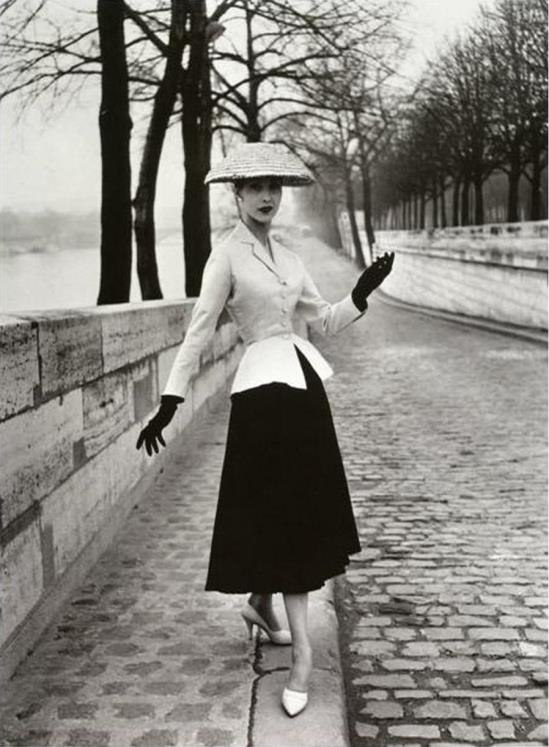
\includegraphics[width=.333\textwidth]{articles/06-vencido-o-new-look-r/01-new-look.jpg}%
        \caption*{Fonte: \textapud[p.~20]{Pochna2000Dior}[p.~58]{MedeirosFl2014Arremedando}.\mybibexclude{Pochna2000Dior}}%
        \label{fig:new-look}%
    \end{figure}%

    Através da imagem acima, percebe-se as características do \textit{new look}: cintura fina e marcada, ancas largas, saia comprida e rodada e chapéu complementar. De acordo com \textcite{MedeirosFl2014Arremedando}, o \textit{new look} foi o primeiro modelo a tomar proporções mundiais, o que se confirma quando se analisa periódicos como os que circularam no estado do Rio Grande do Norte, como o \textit{Diário de Natal}, fotografias do período e até mesmo revistas que não desembocavam nas localidades mais remotas, a exemplo da revista \textit{O Cruzeiro}, também fonte para este estudo.

    Neste sentido, a tendência que transcendeu a década de 1950 e repercutiu em temporalidades posteriores, como a década de 1960, com algumas variações, era formado por:

    \begin{quotation}
        \noindent{}os corpetes eram armados com barbatanas e, a partir de cinturas muito justas, abriam-se amplas saias, lembrando as corolas das flores. As saias poderiam ser pregueadas, franzidas, drapeadas ou nesgadas, sempre forradas com tule para darem o efeito de armação, resultando na forma corolácea de uma cúpula \cite[p.~116]{MedeirosFl2014Arremedando}.
    \end{quotation}

    Portanto, através das palavras de Medeiros Filho infere-se que a coleção tinha inspiração nas corolas de flores, prezando pela demarcação das formas femininas a partir de corpetes e quadris apertados, os quais definiam o ideal corpóreo das mulheres, em consonância com a inspiração de Dior que rememorava o século XIX, sobretudo com as anquinhas usadas por baixo das saias rodadas. 

    \begin{wrapfigure}{o}[\dimexpr \marginparsep+\marginparwidth]{0pt}%
        \begin{minipage}[b]{\marginparwidth}
            \caption{Reportagem ``Os modistas francezes de\-cre\-tam a morte do `New Look' e lançam o `New New'{}''.}
            \caption*{Fonte: Biblioteca Nacional, Brasil (Hemeroteca Digital) --- Diário de Natal, ano 1948, ed. 01658, 26 set. 1948.}
            \label{fig:morte-new-look}
        \end{minipage}
        \hspace{\marginparsep}
        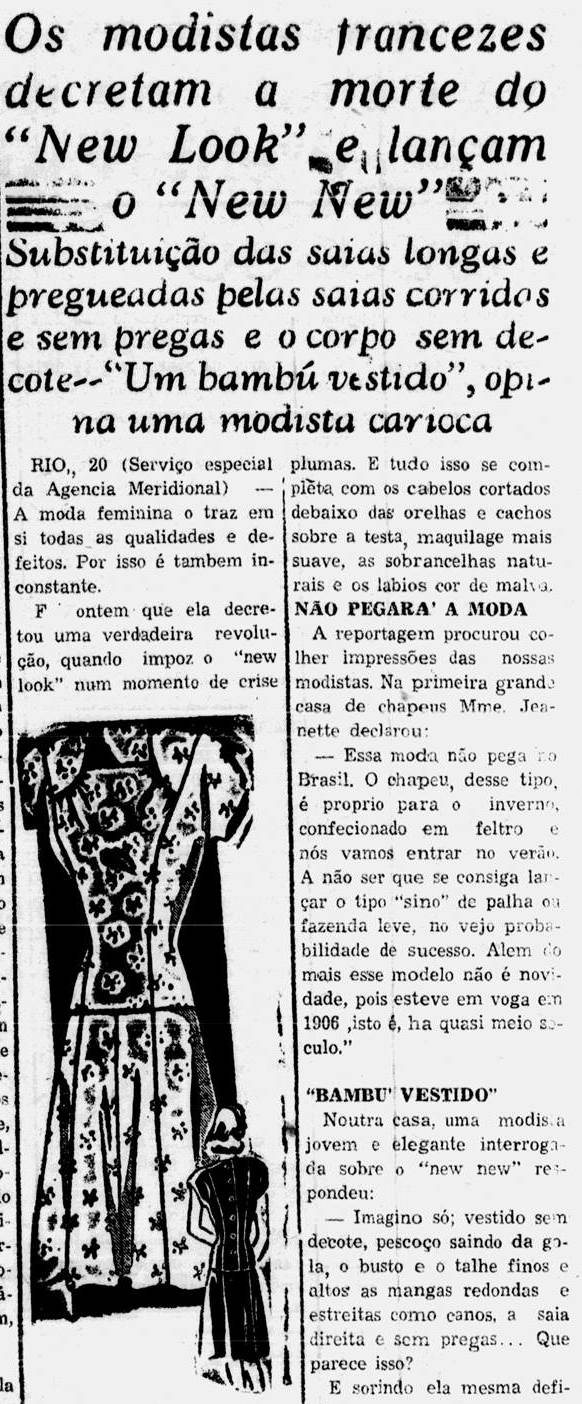
\includegraphics[height=25\baselineskip]{articles/06-vencido-o-new-look-r/02-morte-new-look.jpg}
    \end{wrapfigure}%

    \nocite{ModistasFrancezes1948}

    Deste modo, ainda que houvesse revolucionado não somente as formas estéticas, Dior conseguiu transformar o sistema da moda. Em consonância, a partir do \textit{new look} conseguiu inimigos, resistentes não apenas às suas modas escandalosas, rodadas e exacerbadamente femininas, mas resistentes a pessoa de Christian Dior, como faz refletir o título do presente texto ``resistências femininas a Christian Dior e as suas modas'', como foi percebida pelo jornal \textit{Diário de Natal}. Tratando-se das resistências, o jornal apresenta principalmente acerca dos problemas econômicos, questão trabalhada a seguir.  

    Entre as páginas natalenses, apre\-sen\-ta\-ram-se as mais diversas explicações para que as mulheres não adotassem o novo estilo, influenciadas pelas moças de Paris, de Nova York e do Rio de Janeiro. Dentre os motivos, o clima e as condições climáticas do Brasil. Chamou a atenção que as matérias, sobretudo as primeiras analisadas, já entoavam oposições ao modismo, como no caso da reportagem que retratava a morte do \textit{new look} e o nascimento do \textit{``new new''}, o novo estilo era uma resposta dos estilistas franceses a Christian Dior (figura \ref{fig:morte-new-look}): ``o traje completo quer modificar inteiramente as novas linhas da elegância feminina: vestido sem decote, pescoço saindo da gola, busto alto, talhe alto e fino, as cadeiras bem amplas, as mangas redondas e estreitas e a saia direita sem pregas''. Por meio do fragmento da reportagem, é possível identificar aspectos como a mudança, mais uma vez da silhueta feminina, com mangas bufantes, saias retas, assim como o discurso acerca da elegância a qual o \textit{``new new''} traria para as moças, onde é possível perceber uma crítica escancarada a Dior e ao \textit{new look}.

    \begin{wrapfigure}{o}[\dimexpr \marginparsep+\marginparwidth]{0pt}%
        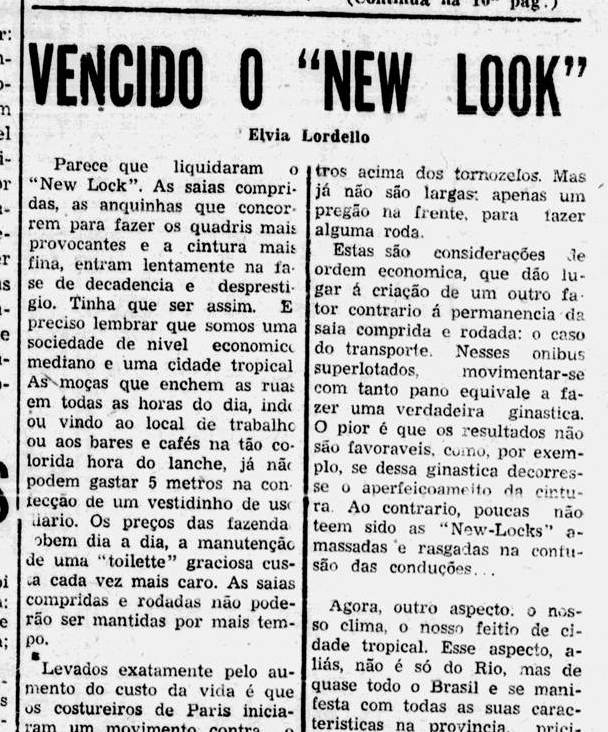
\includegraphics[height=14\baselineskip]{articles/06-vencido-o-new-look-r/03-vencido-new-look.jpg}
        \hspace{\marginparsep}
        \begin{minipage}[b]{\marginparwidth}
            \caption{Artigo ``Vencido o `New Look'{}''.}
            \caption*{Fonte: Biblioteca Nacional, Brasil (Hemeroteca Digital) --- Diário de Natal, ano 1949, ed. 01768, 23 jan. 1949.}
            \label{fig:vencido-new-look}
        \end{minipage}
    \end{wrapfigure}%

    A reportagem apresenta o lançamento do modismo supracitado imerso em um contexto econômico caótico em virtude do pós-guerra. Mesmo assim, não foi empecilho para a ditadura da moda, a qual impôs saias compridas e caras. É que a moda então se baseava no capital, produzindo modelos caros e não se preocupando com a elegância feminina.

    Em 1949, dois anos após a apresentação do \textit{new look}, era publicada uma reportagem intitulada ``Vencido o New Look'' (figura \ref{fig:vencido-new-look}), escrita por Eva Lordello. De acordo com a matéria, o \textit{new look} estava saindo de moda, pois as anquinhas estavam sendo abandonadas junto das saias compridas que davam às mulheres cinturas mais finas, é possível perceber que a repórter ``agradeceu'' por essa moda estar indo embora por dois fatores: a questão econômica, que o Brasil e Natal ocupavam: ``os preços das fazendas sobem dia a dia, a manutenção de uma \textit{`toillete'} graciosa custa cada vez mais caro. As saias compridas e rodadas não poderão ser mantidas por mais tempo''. E as condições tropicais não só do país como da capital, quando argumentou que para o \textit{new look} eram necessários 5 metros de tecido, como moças tropicais e de situação econômica mediana, talvez não conseguissem usar esses vestidos diariamente.

    \textcite{Lordello1949Vencido} ainda argumentava que o modismo estava fora de moda, até mesmo em Paris, pois a tendência requeria muitos metros de tecido: ``tantas saias, tantos babados, tantas rendas e tantas fitas, um Deus nos acuda de accessorios quase inuteis, tirando a graciosidade da silhueta, ou deformando outras de si mesmas, propensas a poucos panos''. Percebe-se a apatia da repórter em relação ao \textit{new look}, no fragmento em questão o qual ela expressava sua insatisfação quando argumentou acerca dos excessos, que acabavam por tornar aquela peça feia, consequentemente a mulher também enfeirar-se-ia. Mediante Lordello, as mulheres queriam sempre o novo, o contemporâneo, e aqueles modelos de Christian Dior já estavam ultrapassados. Em consonância com a overdose estética que o estilista havia lançado dois anos atrás, Loredello continuava suas resistências argumentando que as saias amplas eram empecilhos para o transporte: ``nesses onibus superlotados, movimentar-se com tanto pano equivale-se a fazer uma verdadeira ginastica''; percebe-se a dificuldade até de se movimentar com tal criação extravagante.

    Outro exemplo das críticas a Dior, que esteve presente no jornal, foi a de Bárbara \textcite{Miller1953Luta}. A repórter retratava sobre a resistência das secretárias nova-iorquinas, face à última moda lançada pelo estilista, a saia recém-lançada, que era muito curta: ``'só temos duas mãos: uma para escrever e outra para segurar a saia e cobrir os joelhos''. Nesta matéria, é possível perceber que Dior estava retornando à moda de 1920, com saias mais curtas, com 40 cm do chão, evidenciando que a matéria retratava a resistência feminina não somente ao \textit{new look}, mas a Christian Dior e às suas criações. As novas saias estavam mais curtas, e a jornalista indagava acerca da receptividade, se o estilista conseguiria lançar as saias no mercado e se estas seriam bem aceitas pelas moças, tendo em vista o tamanho das peças.  

    Na mesma reportagem aparece uma ``entrevista'' com Christian Dior, ou ao menos perguntas para o estilista, sobre as críticas que estava recebendo. Assim, questionado sobre a inovação estética, o costureiro disse que se vivia uma nova era. A resistência foi sentida não apenas pelas natalenses, mas por outros modistas (não foi informado se eram de Paris ou de outros lugares), que se mostraram apáticos à criação do francês. Como as críticas direcionavam-se às saias curtas, a reportagem acreditava que essa moda não pegaria, sobretudo pelas secretárias de Nova York para quem as novas peças atrapalhavam o trabalho.  

    Portanto, as tramas do sistema da moda, durante os anos de 1948--53, estavam desfavoráveis não somente ao \textit{new look}, criação de Christian Dior, mas ao estilista e também às modas por ele produzidas. Estas resistências serão apresentadas outras, ainda que dialoguem diretamente com o \textit{new look}, mas que não receberam dos jornais a expressão ``new look'', podemos inferir que trata-se do modismo criado pelo francês, pelas características principalmente das saias rodadas. Neste sentido, soma-se à tessitura do texto em questão, as apropriações das moças, presentes principalmente na seção ``Notícias da Moda'', entre os anos de 1948--1950, bem como as reportagens que retrataram os conflitos entre saias mais curtas e/ou mais compridas. Assim, pode-se inferir que as novas modas, de saias de comprimento reduzido, e as mais alongadas também receberam influências diretas das criações de Dior.  

    A partir das reportagens analisadas, percebe-se que entrava em conflito os gostos e os discursos jornalísticos, para tanto, Calanca acerca do gosto, diz que: ``o gosto, portanto, define-se como faculdade de julgar desinteressadamente um objeto ou uma representação mediante um prazer ou um desprazer'' \cite[p.~93]{Calanca2008Historia}. A partir de Calanca, identifica-se que os embates no tocante ao \textit{new look} em Natal, perpassaram o gosto, das que escreviam as matérias jornalísticas, mas também das moças que faziam o uso do estilo, logo, infere-se que o gosto pelo \textit{new look} variava entre as jornalistas que resistiam e reprovavam a tendência e, sobretudo, as natalenses que adotaram tal moda. Em consonância, insere-se na discussão, o conceito de gosto, amplamente utilizado por Medeiros Filho, quando compreende que as moças em São João do Sabugi não vestiram diretamente o \textit{new look}, mas o arremedaram mediante as suas condições (climáticas, econômicas, culturais).

    \section{Notícias da Moda, uma seção de modos e modas}

    \nocite{NoticiasDaModa1948janeiro}

    Durante os anos de 1948--50 no \textit{Diário de Natal}, as moças que quisessem se informar sobre as efemeridades da moda leriam a seção ``Notícias da Moda'', na página feminina do periódico. Por entre as páginas da seção de modos e modas, as moças atualizar-se-iam acerca das tendências, dos desfiles estrangeiros, dos comprimentos das saias e os conflitos que estes tamanhos ocasionariam. Neste sentido, ainda que os jornais silenciem, nas suas páginas percebeu-se que tal seção vigorou apenas por três anos, pois após 1950 as reportagens sobre moda não apareceram mais naquela coluna, mas dispersas no periódico.

    Outrossim, a seção supracitada servia apenas como informativo no tocante aos modismos e novidades estrangeiras que aportavam em Natal, mas de formadora de opinião sobre o que as moças deveriam vestir. Definia-se o que era considerado atual, os usos que seriam apropriados, as resistências mediante os parâmetros morais e estéticos, se cobririam e se embelezariam a partir das silhuetas retas e esguias ou das amplas e rodadas saias. Pelas páginas, foi possível identificar que o conflito entre o comprimento das saias estava imerso também quando Christian Dior lançou o \textit{new look} o que estendeu as resistências ao estilista e não somente à sua clássica e revolucionária criação. 

    Nas primeiras ocorrências que retratavam sobre as saias curtas e compridas, ainda em 1948, é possível inferir que a dúvida instaurada acerca dos comprimentos, fazia-se presente entre os cortes masculinizados e retilíneos, sem muitas curvas, formando uma silhueta séria e sóbria, ou mais cortes afeminados, enaltecendo a feminilidade, através de ancas, drapeados e saias rodadas. Tais tendências eram importadas de Paris, e ainda que advindas da capital da moda, não agradavam a todos, sobretudo pelo tamanho das saias, mais curtas, pouco abaixo do joelho. Para além das saias, outra tendência que estava acarretando reprovações estéticas era o uso de calças inspiradas nas \textit{maisons} Balmain, Hermés, Lanvin, que apresentavam calças para as mulheres como símbolo de modernidade.

    Tais frivolidades da moda, que desagradavam tantos, eram como as estranhezas do tempo da guerra, com os cortes totalmente diferentes, não eram mais masculinizados e sim com pregas e drapeados, como mostra a reportagem da seção abordada no tópico em questão: ``as prezas, os drapeados são os característicos dessa tendência suntuosa.'' Por meio do fragmento da reportagem, é possível perceber que as novidades eram opostas àqueles que preferiam a simplicidade dos trajes, da silhueta sisuda, evidenciando que a moda não estava sendo bem aceita por todos, pois os novos padrões eram totalmente diferentes dos anteriores, uma verdadeira revolução estética.  

    As tentativas em resgatar o comprimento das saias mais compridas não estavam vigorando, pois era inconveniente para o ano de 1948. Logo, apesar de opostas às saias longas e armadas, o jornal mostrava que as moças não deveriam fazer o uso de saias muito curtas. Entretanto, ``não nos referimos é claro, aos vestidos demasiadamente curtos com que certas senhoras de fartas carnes e de não menos avultadas banhas timbram em usar, dando assim uma demonstração eloquente de falta de tato e de equilíbrio.'' Através do fragmento da reportagem, percebeu-se que, de acordo com o \textit{Diário de Natal}, as mulheres não deveriam usar grandes e compridas saias, tampouco saias muito curtas, que exibissem demais suas fartas carnes. Pela concepção do periódico, o comprimento ideal seria pouco abaixo do joelho, visto que estas saias eram mais confortáveis, e ideais para mulheres que precisavam trabalhar fora de casa, pois não eram complicadas de se movimentarem, além de diferenciarem dos homens já que não eram tão parecidas com as vestes masculinas. É perceptível que o jornal também se colocava no papel de ditar a opinião pública, como o caso de formar o imaginário feminino acerca das roupas mais adequadas para sair de casa e para trabalhar. 

    Ainda sobre a extensão das saias, e em consonância com o corpo feminino, Rosa \textcite{Kaliweyer1948Batalha} em ``A batalha das modas da primavera em Paris'', retratou que ``a linha apresenta-se esguia. A cintura fina e flexível. O busto redondo e alto''. As formas femininas deveriam ser, deste modo, a partir da reportagem, finas com bustos que destacassem os seios e os elevassem. Para além dessas características, na mesma reportagem, Kaliweywer ressaltava que imperava entre as mulheres o uso de saias rodadas, mesmo que algumas usassem as saias mais justas ao corpo, as \textit{godets}\footnote{\textcite{MedeirosFl2014Arremedando} compreende as saias godês, ou \textit{godets}, enquanto fragmentos triangulares do tecido das saias o que as torna mais largas e dão o efeito de saia rodada.} se sobressaíam, percebe-se assim que as resistências a Christian Dior e às suas modas não eram totalmente aplicadas, pois uma de suas criações e disseminações foram as saias \textit{godets}, que segundo a reportagem em questão estavam sendo amplamente apropriadas ``apesar de se verem muitos modelos com saias estreitas, as rodadas predominam e oferecem maior variedade.''\footnote{Ibidem.} Por meio dos amplos usos, o mercado era mais variado para as \textit{godets}.

    Atrelada às saias \textit{godets}, Kaliweyer argumentava que as pregas, pinças e franzidos se combinavam com muitos babados e tecidos, confeccionadas em tafetá, \textit{mousselines}\footnote{Segundo \textcite{MedeirosFl2014Arremedando}, \textit{mousselines} corresponde à tecidos frágeis, utilizados para a feitura de indumentárias íntimas.}, rendas e bordados, em tons pastel de azul e rosa, na reportagem aparece menção às saias que encurtaram em 25 centímetros. É nítida as relações diretas com o modelo de Christian Dior, refletidas nas pregas, rendas, babados assim como no tamanho da saia.

    \nocite{CurtasOuCompridas1948}
    \nocite{NoticiasDaModa1948janeiro}
    \nocite{NoticiasDaModa1948Junho}
    \nocite{DiarioDeNatal1949SemTitulo}

    Em consonância com as noções de saias mais curtas ou compridas, uma reportagem da seção ``Notícias da Moda'', retratava que a moda em 1949 estava sendo diferente das anteriores em virtude das resistências, logo, encontravam-se mulheres com saias rodadas e saias retas, estas últimas não haviam se adaptado ou rendido à moda das primeiras: ``E com os `panneaus'\footnote{Termo em francês que foi usado para referir-se a tecido leve, no caso da reportagem os tecidos das saias.} soltos, drapeados, plissados, notas embelezadouras da silhueta estreita; com a ampliação da saia leva para traz, o que no tailleur, o casaco repete.'' Pode-se perceber que a tendência das pregas estava sendo a preferida entre as mulheres, presentes também nos casacos, sobretudo entre os tailleurs, os quais contrastavam com as saias estreitas. 

    Face ao caráter cíclico da moda, o periódico tratava o retorno à moda dos vestidos com o comprimento abaixo do joelho, onde as mulheres o trajavam exibindo elegância, sobretudo quando eram usados de noite, as saias eram rodadas e estampadas, combinados com um corpete que ajudava na modelação do corpo, os quais tinham Paris como maior centro de referência para a moda brasileira e, no caso de Natal, os arremedos franceses que a capital potiguar fazia em relação à capital francesa. Percebe-se ainda que a moda das saias rodadas ainda imperava, principalmente para as moças irem para os bailes noturnos, a silhueta estava em transformação, transformação que não é especificada pelo jornal. 

    As saias longas não vigoraram por tanto tempo. No começo assim que essas surgiram foram criticadas pelo tanto de pano que necessitavam, impossibilitando os movimentos femininos, os vestidos grandes foram tão revolucionários, pois transformaram a ordem estética vigente por dez anos, que era das saias curtas. Com a Segunda Guerra o cenário indumentário transfigurou-se, visto que o estilista Christian Dior substituiu a masculinidade dos trajes femininos, muito presentes na década de 1940, com o conflito armado tal situação mudou com a volta das saias curtas, assim, ainda que as mulheres não estivessem animadas com a moda, o inverno de 1949, estava chegando e as mulheres precisavam de roupas da moda, moda essa que havia ampliado as possibilidades de saias, \textit{godets}, rodadas, com pregas, lisas, estampadas. 

    As modas estrangeiras eram de vestidos mais compridos, mas quando estes chegavam no Brasil eram arremedados e diminuído, um exemplo das efemeridades e arremedos, como explicitado no fragmento a seguir:

    \begin{quotation}
        O tempo das saias compridas morreu com a falências de certas teorias retrógradas que limitavam á mulher todas as suas possibilidades e aspirações e, compreendendo isso, assim como sendo a aceitação sem raciocínio, de todas as imposições da moda, o índice de uma mentalidade de que elas, de possuídas, ao analisarem por todos os prismas da moda da saia comprida, resolveram protestar, conservando os seus vestidos sincrónicos com a vida dinamica e liberta de certos preconceitos retrógrados que caracterizam nossos dias.
    \end{quotation}

    Pode-se inferir a partir do fragmento de reportagem que as saias compridas eram opressoras das mulheres e dos seus movimentos. Já o abandono de tal tendência e adoção de saias mais curtas poderia significar o abandono de tais opressões que limitavam os movimentos.

    \section{Alguns retoques finais}

    À guisa de conclusão, em função do exposto, compreende-se que as resistências ao new look foram importadas da Europa, dos Estados Unidos, e de outras localidades do Brasil como o Rio de Janeiro, e terminaram por desembocar em Natal, influenciando as leitoras do \textit{Diário de Natal} a se vestirem, comportarem, recusarem e aceitarem certas tendências. Além de tal concepção, é possível argumentar que as resistências ocorreram ao passo de que as apropriações também estiveram presentes na sociedade natalense, pois pelas reportagens foi possível identificar tais conflitos entre as moças que eram contrárias e as que eram favoráveis ao modismo.

    O estilista e costureiro francês Christian Dior foi o principal alvo das críticas e resistências das matérias analisadas na presente exposição pelos seguintes motivos: demanda de muitos metros de tecido para a confecção das amplas e rodadas saias, dificuldade de se movimentar, problemas no transporte público, clima inadequado para o novo modismo. Ainda assim, com tais manifestações avessas a Dior, o estilista consagrou-se no mercado de alta-costura francesa, influenciando o mercado da moda mundial com a combinação de saias \textit{godets}, e \textit{tailleur}. Os escritos acerca da moda eram registrados, sobretudo entre 1948--1950 na seção ``Notícias da Moda'', que era responsável por formar o pensamento relacionado aos novos cortes e silhuetas bem como intervir no cotidiano potiguar.  

    Logo, a história que aqui foi retratada pelo periódico proporciona a compreensão de outras histórias do Rio Grande do Norte, não somente calcadas nos jogos políticos das oligarquias, mas também numa história pelas tramas dos costumes, das costuras, das tendências e efemeridades, evidenciando a necessidade de se conhecer, pesquisar e estudar sobre os discursos da moda, suas possibilidades, e neste caso em específico, as resistências.

    \printbibliography[heading=subbibliography,notcategory=fullcited]

    \hfill Recebido em 15 abr. 2021.

    \hfill Aprovado em 19 abr. 2021.

    \label{chap:vencidonewlookend}

\end{refsection}

\begin{refsection}
    \renewcommand{\thefigure}{\arabic{figure}}
    
    \chapterOneLine{Os caminhos e os desdobramentos da vida, trajetória política e dos discursos e pronunciamentos de Dinarte Mariz}
    \label{chap:caminhosdesdo}
    
    \articleAuthor
    {Larisse Santos Bernardo}
    {Mestranda em História dos Sertões (UFRN-CERES, Caicó). ID Lattes: 8111.2333.0951.3952. ORCID: 0000-0001-8427-7303. E-mail: larissesantosbernardo@yahoo.com.br.}

    \articleAuthor
    {Jailma Maria de Lima}
    {Professora de História do Departamento de História na UFRN-CERES, Caicó. ID Lattes: 7070.0102.8841.6835. ORCID: 0000-0001-8689-1753. Orientadora da referida pesquisa.}

    \begin{galoResumo}
        \marginpar{
            \begin{flushleft}
            \tiny \sffamily
            Como referenciar?\\\fullcite{SelfBernardoAndLima2021}\mybibexclude{SelfBernardoAndLima2021}, p. \pageref{chap:caminhosdesdo}--\pageref{chap:caminhosdesdoend}, \journalPubDate{}
            \end{flushleft}
        }
        O presente trabalho tem por desígnio traçar os percursos analíticos da trajetória de vida e política, como também das reverberações acerca dos discursos e pronunciamentos a partir da figura eminente de Dinarte de Medeiros Mariz. Político este que se firmou no cenário da política nacional e, que por sua vez, deixou marcas registradas na política potiguar a partir de suas raízes no Seridó norte-rio-grandense. Nessa perspectiva o desenvolvimento da narrativa se dará através de um viés que traçará sua vida política mostrando as alianças criadas, os degraus percorridos por Dinarte, levando em consideração que antes de se tornar figura política, ele foi comerciante e agropecuarista, experiências que corroboraram para o seu fortalecimento na vida política. Assim, a partir desses encaminhamentos busca-se concernir o porquê da manutenção no imaginário político e social em torno da figura pública, uma vez que o mesmo conquistou impulsividade pública ocupando vários cargos, entre os quais, prefeito da cidade de Caicó, governador do Estado do Rio Grande do Norte e Senador da República.
    \end{galoResumo}
    
    \galoPalavrasChave{Dinarte Mariz. Vida. Trajetória Política. Discursos.}
    
    \begin{otherlanguage}{english}
    
    \fakeChapterOneLine
    {Ways and unfoldings of Dinarte Mariz's life, political trajectory, speeches, and pronouncements.}

    \begin{galoResumo}[Abstract]
        This work aims to trace the analytical paths of life and politics, as well as the reverberations about the speeches and pronouncements by the eminent figure of Dinarte de Medeiros Mariz. Politician who was established in the national politics scene and, in turn, left his mark etched in the potiguar politics starting from its roots in Seridó of Rio Grande do Norte. In this perspective, the narrative development will take place through a bias that will trace his political life showing created alliances, the steps taken by Dinarte, taking into account that, before becoming a political figure, he was a trader and farmer, experiences that corroborated for strengthening of his political life. Thus, based on these referrals, we seek to concern the reason why the political and social imaginary maintains around that public figure, since he gained public impulsiveness by occupying various positions, among which, mayor of Caicó, governor of the State of Rio Grande do Norte and Senator of the Republic.
    \end{galoResumo}
    
    \galoPalavrasChave[Keywords]{Dinarte Mariz. Life. Political trajectory. Speeches.}
    \end{otherlanguage}

    \section{Introdução}

    O presente trabalho tem por desígnio traçar os percursos analíticos da trajetória de vida e política, como também das reverberações acerca dos discursos e pronunciamentos a partir da figura eminente de Dinarte de Medeiros Mariz. Político este que se firmou no cenário da política nacional e, que por sua vez, deixou marcas registradas na política potiguar a partir de suas raízes no Seridó norte-rio-grandense.  

    Para isso, é necessário primordialmente apresentar a pessoa de Dinarte de Medeiro Mariz\footnote{Ver em: \textcite[p.~220]{Maia2005Dinarte}}, assim registrado, mais conhecido por seu segundo sobrenome Mariz. Observando a vida e sua trajetória política, o artigo intitulado \textit{Período Republicano} da fundação José Augusto, o mesmo descreve que \textit{Dinarte de Medeiros Mariz}, nasceu na Fazenda Solidão em Serra Negra-RN\footnote{[\dots] O professor Vergniaud Lamartine Monteiro explica o nome da região no semi-árido nordestino: ``Os primeiros batedores da região, localizados na fralda sudeste da serra, verificaram serem as suas encostas acentuadas noruegas, as quais davam à serra aquele lugar, ao tempo imerso em vegetação sombria e matarias virgens, um aspecto negro''. Na região, além da vegetação de menor porte, convivem o juazeiro, a oiticica, a jurema, o angico e o pau-d'arco. É o coração do Seridó. \cite[p.~39--40]{Lima2003Solidao}.} no dia 23 de agosto de 1903, filho de Manuel Mariz Filho e de Maria Cândida de Medeiros Mariz o quinto entre quatorze filhos do casal. Seu avô, José Bernardo de Medeiros, foi constituinte em 1891 e ocupou uma cadeira no Senado Federal de 1890 a 1907. Com vinte e um anos de idade, Dinarte Mariz contrai matrimônio com Diva Wanderley, filha de Virgolino Pereira Monteiro, comerciante no setor pecuário e político de Campina Grande-PB.

    Ainda em se tratando sobre a trajetória de vida de Dinarte Mariz, é necessário discorrer brevemente sobre sua escolaridade, uma vez que, o mesmo não chegou a cursar o ensino superior, o que levou a afirmar várias vezes que ele era formado na escola da vida. Assim, Mariz teve:

    \begin{quotation}
        O seu primeiro professor foi Arthéfio Bezerra, no Grupo Escolar Coronel Mariz, em Serra Negra. Estudou aritmética, leitura e análise sintática, que na época se dizia análise lógica. Foi para Caicó e, no Grupo Escolar Senador Guerra, concluiu o primário com o professor Pedro Gurgel de Amaral. Foi sempre o primeiro aluno da classe. Lá, aprendeu cantar o hino de Sant'Ana, a história da cidade, viu a beleza plástica no desfile da irmandade do Rosário, viveu o encanto místico da região. \cite[p.~41]{Lima2013Sertao}.
    \end{quotation}

    Ao concebermos sua descendência política, compreendemos que a mesma integra parte de uma parentela que conseguiu se manter no poder. Segundo Linda Lewin:

    \begin{quotation}
        A parentela está associada a uma organização social e estava subjacente à base da rede de parentes e amigos de um político. O núcleo dos seguidores políticos que a ele se vinculam de maneira personalística, constituindo os membros de sua parentela. Os membros deste grupo de base familiar organizavam localmente o eleitorado para fornecer-lhe os votos, defendiam seus interesses partidários em seu município natal e os serviam lealmente em que ingressavam por nomeação. \cite[p.~113]{Lewin1993Politica}.
    \end{quotation}

    Antes de adentrarmos sobre a vida política de Mariz, é de bom grado explanar, por sua vez, a ocupação do mesmo antes de enveredar na carreira política. Então, Dinarte de Medeiros Mariz foi um remanescente da cultura algodoeira e da pecuária, ou seja, um comerciante que por sua vez comandava política e economicamente a região do Seridó. Mediante esse contexto, ficou evidente que sucedeu partir da região habitada pelo referido acima, precisamente, da cidade de Caicó, que fica localizada no Estado do Rio Grande do Norte (RN), na região Seridó\footnote{O Seridó é uma civilização solidária. Desde que consideremos civilização num conceito menos amplo que os que se aplicam à nação. Região desfavorecida pelo clima, nuvens e chão, é beneficiada pelo homem, sua vontade, sua decisão. E pelas bênçãos de Deus. \cite[p.~57]{Lima2003Solidao}.

    A civilização do Seridó é uma herança cultural que se baseia em vontade coletiva, impossível de ser medida, incomensurável. Tem por base suas propriedades rurais que são historicamente unidades autônomas, sustentadas pela produção de gado, pela produção agrícola e pelos peixes que povoam as centenas de pequenos açudes cavados pela mão do homem. \cite[p.~57--58]{Lima2003Solidao}. }. Assim, foi através desse lugar que propiciou a criação de um grupo oligárquico\footnote{A oligarquia se compõe necessariamente daquele grupo minoritário que, por meio da divisão organizacional do poder, logra ocupar posições institucionais que lhe permitem tomar decisões que afetam os interesses coletivos de forma infensa a controle. \cite[p.~48]{Couto2012Oligarquias}.

    Essa concepção da ``classe política'' é importante na construção de um conceito descritivo de oligarquia porque é ela que permite pensar nos ``oligarcas'' como um grupo de poder específico e na ``oligarquia'' como a forma de predomínio desse grupo, que se distingue dos demais não por sua origem de classe, mas pelo papel organizacional específico que desempenha. \cite[p.~48]{Couto2012Oligarquias}.
    
    Aqueles que se profissionalizam como dirigentes partidários, retirando dessa condição seus ganhos e seu status, mas também desfrutando de condições diferenciadas de poder organizacional, rapidamente adquirem as condições para se formarem uma oligarquia. O que permite a sua transformação em oligarcas não é apenas a sua conversão em profissionais da política (embora esta seja uma condição necessária), mas a detenção de um poder na organização não desfrutado pelos demais. Noutros termos, a organização é capturada pelos dirigentes, e isto é o que lhes converte em oligarcas. \cite[p.~48]{Couto2012Oligarquias}.} --- familiar, que apareceu com o desenvolvimento da cotonicultura, representado pelo seu líder maior, o coronel, José Bernardo de Medeiros.\footnote{Ver em: \textcite[p.~187]{Lamartine2003Personagens}}

    Seu primeiro ato político se deu no ano de 1927, com apenas 24 anos de idade, quando solicitou a intendência, ou seja, a prefeitura da cidade de Serra Negra do Norte. Esta reivindicação, por sua vez, não obteve resultados, uma vez que, a família na época pensou que não era a vez dele, fato que o deixou bastante angustiado, caso este que foi confirmado por Olavo de Medeiros Filho:

    \begin{quotation}
        Conversando certa vez no alpendre da fazenda Solidão, perguntei a Dinarte Mariz quais os motivos que o teriam levado a participar da Revolução de 1930, sendo ele parente e conterrâneo do Governador Juvenal Lamartine de Faria, deposto pela referida Revolução, dando uma risada, afirmou-me Dinarte Mariz que tudo teria origem em um pedido que ele fizera a Juvenal Lamartine propondo-se a ser prefeito de sua querida cidade Serra Negra do Norte. O pedido provocou gargalhadas em Juvenal, que descartou a pretensão do parente, pessoa que, segundo ele, não preenchia as condições exigidas para ocupar a chefia da edilidade. \cite[p.~166]{Lima2003Solidao}.
    \end{quotation}

    Então em 1929, durante o governo de Washington Luís (1926--1930), era comerciante de algodão em Caicó (RN), e ingressou na Aliança Liberal\footnote{A Aliança Liberal foi formada em 1929 por setores dissidentes da oligarquia paulista e mineira insatisfeita com o sistema excludente. (SPINELLI, sd., p. 15). } --- agrupamento político oposicionista formado basicamente pelos partidos republicanos mineiro e gaúcho, pelo Partido Democrático (PD) paulista e pelo situacionismo paraibano apoiando a candidatura de Getúlio Vargas e João Pessoa à presidência e vice-presidência da República nas eleições de março de 1930. Contudo, o candidato eleito foi Júlio Prestes, apoiado pelo presidente Washington Luís. A derrota de Vargas, aliada ao assassinato de João Pessoa no mês de julho em Recife, provocou a eclosão do movimento revolucionário de outubro de 1930, ao qual o então Dinarte Mariz sob o comando do capitão do exército Abelardo Torres da Silva Castro participou da revolução no Rio Grande do Norte. 

    Adentrando nos caminhos políticos já introduzidos anteriormente acima, Dinarte de Medeiros Mariz deu continuidade aos seus engajamentos na política, uma vez que, passou a se posicionar favoravelmente a Revolução de 1930, participou ativamente de todos os movimentos armados a posteriori como a Revolução Constitucionalista de 1932 em São Paulo, a Intentona Comunista de 1935\footnote{Em março de 1935 foi criada no Brasil a Aliança Nacional Libertadora (ANL), organização política cujo presidente de honra era o líder comunista Luís Carlos Prestes. Inspirada no modelo das frentes populares que surgiram na Europa para impedir o avanço do nazi-fascismo, a ANL defendia propostas nacionalistas e tinha como uma de suas bandeiras a luta pela reforma agrária. Em agosto, a organização intensificou os preparativos para um movimento armado com o objetivo de derrubar Vargas do poder e instalar um governo popular chefiado por Luís Carlos Prestes. Iniciado com levantes militares em várias regiões, o movimento deveria contar com o apoio do operariado, que desencadearia greves em todo o território nacional. O primeiro levante militar foi deflagrado no dia 23 de novembro de 1935, na cidade de Natal. No dia seguinte, outra sublevação militar ocorreu em Recife. No dia 27, a revolta eclodiu no Rio de Janeiro, então Distrito Federal.}, combatendo os comunistas no Rio Grande do Norte, esteve presente nas conspirações contra a ditadura varguistas e outro momento importante foi a participação da fase preparatória da Revolução de 1964. Dessa forma, segundo Jailma Maria de Lima ``[\dots] A ênfase dada a sua própria trajetória é a de um revolucionário, que articula nos bastidores, mas também que está na linha de frente de alguns episódios [\dots]''. \cite[p.~11]{Lima2013Memoria}.

    \section{Dinarte Mariz: vida, político e seus discursos}

    Dinarte Mariz assim como ficou conhecido, ingressou na vida pública com seu primeiro cargo político como prefeito da cidade de Caicó, aos 27 anos de idade, cargo do qual se afastou após dois anos em face de seu apoio ao Movimento Constitucionalista de 1932, o que lhe valeu três prisões no Rio de Janeiro. Como homem bem articulado e inquieto que era, de volta ao seu estado natal fundou o jornal ``A Razão'' e foi um dos fundadores do Partido Popular ao tempo em que prosperavam seus negócios com o algodão. Mediante ao desenvolvimento do mesmo nos atos políticos, e através de seu forte desempenho como figura política exerceu o mandato de senador por quatro vezes, tendo sido a última por escolha indireta do presidente da República. Nessa linha de influência por mais de uma vez, foi 1º secretário do Senado, um dos cargos mais importantes daquela Casa legislativa. 

    Nessa trajetória e dentro desse contexto, Dinarte Mariz não parou e seguiu em frente com suas articulações e artimanhas para conseguir seus objetivos. Com alianças familiares e proximidades políticas, principalmente, com o seu primo José Augusto Bezerra de Medeiros\footnote{Este por sua vez, ex-governador do Estado do Rio Grande do Norte e com forças políticas na região do Seridó.}, fundou o partido da União Democrática Nacional (UDN), este instituído oficialmente em nível nacional em 7 de abril de 1945, que por sua vez, congregava forças diversas e até antagônicas, em uma extensa frente de oposição ao governo Vargas. Sobre a composição e as alianças do partido:

    \begin{quotation}
        Presidente: José Augusto; vice-presidente: Dinarte Mariz; secretários: Luiz Antonio dos Santos Lima e Djalma Marinho; tesoureiro: Severino Alves Bila. O diretório possuía ainda uma comissão de articulação com o interior e uma comissão de imprensa. Os Diários Associados estavam representados por Edilson Varela e Américo de Oliveira Costa. (O Diário, Natal, 6 de jul. 1945, p. 1).
    \end{quotation}

    Então, nesse período para além da criação e fundação do partido da UDN, Dinarte Mariz lançou-se a candidato ao Senado pela UDN, este por sua vez, não alcançou êxito no pleito eleitoral de 1945. Portanto, Dinarte Mariz foi um homem destemido, com personalidade forte e que não media esforços para alcançar seus objetivos. No ano de 1950 lança sua candidatura ao governo do Estado do Rio Grande do Norte, mas, em acordo com José Augusto Varela não concorreu as eleições, e sim, voltando a concorrer ao Senado Federal na legenda da UDN, que por sua vez, saiu novamente derrotado.  

    No pleito de 1954 Dinarte Mariz, favorecido por um acordo firmado com seu adversário, o pessedista Georgino Avelino, elegeu-se senador pelo Rio Grande do Norte como candidato da coligação UDN-PSP-PSD. Pouco tempo depois de assumir a cadeira como senador, Mariz em fevereiro de 1955 lançou sua candidatura ao governo do Estado do RN com o apoio do Presidente da República João Café Filho, obtendo resultados positivos. Portanto, no pleito de outubro de 1955 foi eleito governador do Rio Grande do Norte.\footnote{Disponível em \url{http://www.fgv.br/cpdoc/acervo/dicionarios/verbete-biografico/dinarte-de-medeiros-mariz}. Acesso em 03 abr. 2021.}

    A partir desse contexto, outro fator importante ao se debruçar e dialogar é acerca de outros rumos que desembocaram na trajetória política de Mariz. É nessa perspectiva que cabe aqui abordar o que existiu de desavenças e disputas no Rio Grande do norte. Nesse contexto, Dinarte Mariz foi o precursor de uma disputa ferrenha que existe no Rio grande do Norte, rivalidade essa conhecida através dos partidos, Vermelho x Verde. A origem desta rixa de cores de partido veio na década de 60, quando o Governo do Estado foi disputado por Aluízio Alves e Dinarte Mariz, período que surgiu a Ditadura Militar e, consequentemente, os partidos MDB e Arena. Portanto, partindo dessa premissa o referido político se constituiu de forma precisa com objetivos formados que permitiu alcançar visibilidade não somente na política como também construindo uma representação de homem do povo. Com base em Chartier:

    \begin{quotation}
        As percepções do social não são de forma alguma discursos neutros: produzem estratégias e práticas (sociais, escolares, políticas) que tendem a impor uma autoridade à custa de outros, por elas menosprezados, a legitimar um projecto reformador ou a justificar para os próprios indivíduos, as suas escolhas e condutas. [\dots] As lutas de representações rem tanta importância como as lutas econômicas para compreender os mecanismos pelos quais um grupo impõe, ou tenta impor, a sua concepção do mundo social, os valores que são os seus, e o seu domínio. Ocupar-se dos conflitos de classificações ou de delimitações não e, portanto, afastar-se do social --- como julgou durante muito tempo uma história de vistas demasiado curtas ---, muito pelo contrário, consiste em localizar os pontos de afrontamento tanto mais decisivos quanto menos imediatamente materiais. \cite[p.~17]{Chartier1990Historia}.
    \end{quotation}

    Ao discorrer e se propor analisar a construção da representação da figura pública do ex-governador do Rio Grande do Norte e do ex-senador da República, que por sua vez ficou viva nos seridoenses e potiguares, faz-se necessário discorrer a respeito do conceito de representação desenvolvido por Roger Chartier. Para isso, Chartier aborda o conceito de representação coletiva, ele destaca que ambos se associam a três aspecto com o mundo social:

    \begin{quotation}
        Primeiro, o trabalho de classificação e de recorte que produz as configurações intelectuais múltiplas pelas quais a realidade é contraditoriamente construída pelos diferentes grupos que compõem uma sociedade; em seguida, as práticas que visam a fazer reconhecer uma identidade  social, a exibir uma maneira própria de estar no mundo, a significar simbolicamente um estatuto e uma posição; enfim, as formas institucionalizadas e objetivadas graças às quais ``representantes'' (instâncias coletivas ou indivíduos singulares) marcam de modo visível e perpetuado a existência do grupo, da comunidade ou da classe. \cite[p.~73]{Chartier1990Historia}.
    \end{quotation}

    Na busca do entendimento das representações, a história cultural afasta-se de uma história social baseada nas lutas econômicas, e busca estudar a sociedade das estratégias baseadas simbólicas manifestadas pelas classes, grupos e meios sociais. Sobre o conceito de representação, vemos que a princípio demostrava o que estava ausente, posteriormente vemos a associação dessa ao que está presente. Sobre a função da representação, o autor aborda que:

    \begin{quotation}
        Todas visam, com efeito, a fazer com que a coisa não tenha existência senão na imagem que a exibe, com que a representação mascare ao invés de designar adequadamente o que é seu referente. A relação de representação é assim turvada pela fragilidade da imaginação, que faz com que se tome o engodo pela verdade, que considera os sinais visíveis como indícios seguros de uma realidade que não existe. Assim desviada, a representação transforma- se em máquina de fabricar respeito e submissão, em um instrumento que produz uma imposição interiorizada, necessária lá onde falta o possível recurso à força bruta. \cite[p.~75]{Chartier1990Historia}.
    \end{quotation}

    Para além da construção que se edificou de Dinarte Mariz e a priori discutida, um outro fator importante a respeito da conjuntura política nos pleitos eleitorais são os discursos e pronunciamentos feitos pelo então estadista Mariz. São diversos momentos que observamos o posicionamento político do qual Dinarte possuiu, uma vez que, o mesmo em uma de suas várias entrevistas que deu, diz a seguinte frase: ``O mundo é grande de se ver e eu já vi de tudo. Mas eu vejo tudo a partir de Caicó''\footnote{Vem em: \textcite[p.~70]{Lima2003Solidao}}. Com essa frase ele quis dizer que mesmo sendo um homem viajado, conhecedor do mundo não esqueceu o lugar que lhe ensinou a voar por outros ares, assim não desmemoriando suas raízes. 

    Para compreendermos o tema acerca da construção e a trajetória político e social de Dinarte Mariz, é por sua vez necessário versar acerca dos seus pronunciamentos e posicionamentos políticos para com o povo potiguar. Para tanto, é imprescindível que se tenha um olhar voltado para os discursos, uma vez que, os mesmos perpassam pela sociedade e são entendidos e assimilados de formas diferentes, de maneira que se tem a necessidade de serem abordados e explorados para que possam, por sua vez, servirem de elementos textuais e embasamento para o desenvolvimento na composição dos caminhos percorridos e alcançados pelo referido político Dinarte Mariz. 

    Nesse contexto, pensar as sociedades e seus diferentes discursos produzidos é segundo Foucault ``[\dots] ao mesmo tempo controlada, selecionada, organizada e redistribuída por certo número de procedimentos que têm por função conjurar seus poderes e perigos, dominar seu acontecimento aleatório, esquivar sua pesada e temível materialidade''. \cite[p.~8--9]{Foucault1996Ordem}. Isso parte da premissa da qual temos conhecimento da nossa sociedade e de que há posicionamentos de exclusão e de impedimentos quanto aos posicionamentos de um determinado discurso, visto que nem todos tem o direito de dizer tudo, como também falar de tudo em qualquer âmbito.  

    Então diante dessa conjuntura, a sociedade se priva de pôr em prática certos tipos de discursos uma vez que elas se comportam de maneira em que estão pautados os discursos que são favoráveis a determinado tipo de assunto. Então, segue assim um ritual de direito privilegiado ou de exclusão quanto ao sujeito que quer falar, e esta exclusão da qual se encontra dentro dos discursos é compreendida por Foucault como um tipo de interdição. Dentro desse caminho de afastamento e o seu ligamento com o impedimento, é possível observar que tais discursos estão embasados e voltados para a sexualidade, como também sobre política. Segundo Foucault:

    \begin{quotation}
        [\dots] como se o discurso, longe de ser elemento transparente ou neutro no qual a sexualidade se desarma e a política se pacifica, fosse um dos lugares onde elas exercem, de modo privilegiado, alguns de seus mais temíveis poderes. Por mais que o discurso seja aparentemente bem pouca coisa, as interdições que o atingem revelam logo rapidamente, sua ligação com o desejo e com o poder. Nisto não há nada de espantoso, visto que o discurso --- como a psicanálise nos mostrou --- não é simplesmente aquilo que manifesta (ou oculta) o desejo; é, também, aquilo que é o objeto do desejo; e visto que --- isto a história não cessa de nos ensinar --- o discurso não é simplesmente aquilo que traduz as lutas ou os sistemas de dominação, mas aquilo porque, pelo que se luta, o poder do qual nos queremos apoderar. \cite[p.~9--10]{Foucault1996Ordem}.
    \end{quotation}

    Ainda em se tratando da análise do discurso, outro ponto discorrido por Foucault associado ao discurso é por sua vez, o ato de exclusão dos discursos, uma vez que, este está na oposição entre o verdadeiro e o falso. Essa problematização aparece a partir do momento em que surgem questionamentos acerca do qual foi, qual é através dos levantamentos sobre os discursos, e estes no que lhes diz respeito estiveram presentes por vários séculos da nossa história. Então, segundo Foucault ``[\dots] é um tipo de separação que rege nossa vontade de saber, então é talvez algo como um sistema de exclusão (sistema histórico, institucionalmente constrangedor) que vemos desenhar-se''. \cite[p.~14]{Foucault1996Ordem}. Dessa forma, a exclusão e a separação se constituíram com total certeza, isso com base nos discursos dos poetas gregos do século VI que buscavam a veracidade dos discursos.

    \begin{quotation}
        [\dots] o discurso verdadeiro no sentido forte e valorizado do termo, o discurso verdadeiro pelo qual se tinha respeito e terror, aquele ao qual era preciso submeter-se porque ele reinava, era o discurso pronunciado por quem de direito e conforme o ritual requerido; era o discurso que pronunciava a justiça e a atribuía a cada qual sua parte; era o discurso que, profetizando o futuro, não somente anunciava o que ia se passar, mas contribuía para a sua realização, suscitava a adesão dos homens e se tramava assim com destino. [\dots] Hesíodo e Platão uma certa divisão e estabeleceu, separando o discurso verdadeiro e discurso falso; separando nova visto que, doravante, o discurso verdadeiro não é mais o discurso precioso e desejável, visto que não é mais o discurso ligado ao exercício do poder. \cite[p.~14--15]{Foucault1996Ordem}.
    \end{quotation}

    Nessa perspectiva, para além das análises acerca dos discursos com base na exclusão, interdição e separação a partir das problematizações dos mesmos através dos discursos do exterior e do interior, Foucault aponta que tem outra existência de um grupo do qual está presente nos seus procedimentos, e este por sua vez, proporciona o controle dos discursos, não no ponto de controlar o seu poder e nem de conjurar suas aparições, mas ``[\dots] trata-se de determinar as condições de seu funcionamento, de impor aos indivíduos que os pronunciam certo número de regras e assim de não permitir que todo mundo tenha acesso a eles. [\dots] ninguém entrará na ordem do discurso se não satisfazer a certas exigências ou se não for, de início, qualificado para fazê-lo''. \cite[p.~37]{Foucault1996Ordem}.

    Dessa forma, as análises e abordagens pautadas por Michel Foucault discorre sobre os discursos presentes nas diferentes sociedades a partir de suas várias vertentes como a exclusão, a interdição, a separação e os seus procedimentos de como eles devem ser vistos e analisados. Diante disso, Foucault mostra que:

    \begin{quotation}
        O discurso nada mais é do que a reverberação de uma verdade nascendo diante de seus próprios olhos; e, quando tudo pode, enfim, tomar a forma do discurso, quando tudo pode ser dito e o discurso pode ser dito a propósito de tudo, isso se dá porque todas as coisas, tendo manifestado e intercambiado seu sentido, podem voltar à interioridade silenciosa da consciência de si. \cite[p.~49]{Foucault1996Ordem}.
    \end{quotation}

    Portanto, os discursos seguem o caminho da verdade a qual se encontra dentro de qualquer manifestação das sociedades que os utilizam para demonstrar seus posicionamentos e ensejos de uma determinada situação. Assim, pode-se dizer que todo discurso tem seu próprio significado. 

    Atrelado aos discursos e pronunciamentos de Dinarte Mariz, no livro intitulado ``Dinarte Mariz vida e luta de um potiguar'' de Agaciel da Silva Maia, traz em seu contexto os memoráveis discursos feitos no Senado Federal, dos quais muito bem elogiado pelo referido autor, e que tem como conteúdo os mais diversos que são entre eles: reverenciando a memórias de ex-companheiros políticos, questões voltadas para a seca no Nordeste, bem como a problematização da economia nordestina e por fim comemorações aos 80 anos do mesmo e da criação da Universidade Federal do Rio grande do Norte.\footnote{``[\dots] ano de 1958 tornar-se-ia um marco referencial na cultura e na educação norte-rio-grandense, pois foi no dia 5 de junho desse ano que Dinarte Mariz criou a Universidade Do Rio Grande do Norte, depois federalizada. E não hesitou em construir modernos centros educacionais em Mossoró e em Caicó, dotando-os dos mais avançados recursos pedagógicos da época.'' \cite[p.~38]{Maia2005Dinarte}.} Assim, diz Dinarte:

    \begin{quotation}
        Devo dizer a todos que esta casa foi para mim mais do que uma universidade, porque talvez se tivesse passado por uma universidade, não teria conseguido aprender tanto, receber tantos ensinamentos capazes de me tornar um servidor, um cativo da coisa pública, em defesa do povo brasileiro e, sobretudo, da democracia, sempre cambaleante, que nos oferece momentos, às vezes, de euforia, mas que foge quando pensamos em construir um patrimônio para as gerações que vêm. \cite[p.~173--174]{Maia2005Dinarte}.
    \end{quotation}

    Dinarte Mariz, em seus pronunciamentos trazia também um discurso que pairava críticas e questionamentos para os seus colegas políticos, dos quais apresentava diretamente ao Senado Federal, quando assim apontava que todos aqueles que faziam parte daquela referida casa deveriam lutar e buscar o melhor para o povo e para o Brasil, e não serem apenas aqueles políticos individualistas. Assim em um de seus discursos no Senado Federal diz:

    \begin{quotation}
        Congresso amortecido não é congresso; Congresso que briga por coisas pequeninas, sem pensar no futuro do país, não é congresso; Congresso só se afirma quando defende idéias, princípios e as grandes causas quando a nação está em risco. Este é o Congresso que eu gostaria de ver. Este é o Congresso que nós precisamos, nesta hora, convocar. Os partidos políticos estão aí, as brigas são internas, mas há uma coisa maior do que as brigas dentro dos partidos: é o interesse maior, é o interesse da Nação. Porque se não nos capacitarmos disso, pior do que tem acontecido acontecerá.  E então nós cairemos diante do povo, sem poder dar uma explicação e muito menos encontrar caminhos para que, amanhã o povo possa crer e voltar as vistas para nos apoiar, prejudicando as gerações que hão de chegar para a grande caminhada do futuro. \cite[p.~185]{Maia2005Dinarte}.
    \end{quotation}

    Diante disso, dialogando com Foucault a partir do conceito de discurso por ele desenvolvido, ao se deparar com a apropriação do discurso, vemos que Foucault cita a educação como sendo um dos veículos dessa manifestação, tendo vista que é um modo ``democrático'' de ventilar os pensamentos e embates políticos de determinadas épocas e espaços. Assim, o autor completa o raciocínio com um pensamento que ``todo o sistema de educação é uma maneira política de manter ou de modificar a apropriação dos discursos, com os saberes e os poderes que eles trazem consigo'' \cite[p.~44]{Foucault1996Ordem}.

    Portanto, nesse mesmo contexto, Foucault analisa o ritual de ventilação das palavras, que por sua vez, o autor aponta que as sociedades do discurso e os grupos doutrinários andam imbricados, servindo assim de apoio um para o outro, para poderem alcançar o objetivo maior que é as apropriações sociais desses pensamentos considerados verdadeiros. Buscando a definição do discurso, o autor mostra que esta parte da leitura do mundo, ou seja, é mesmo a releitura dos pensamentos que circulam sobre a sociedade. Desse modo, vemos que:

    \begin{quotation}
        O discurso nada mais é do que a reverberação de uma verdade nascendo diante de seis próprios olhos; e, quando tudo pode, enfim, tomar a forma de discurso, quando tudo pode ser dito e o discurso pode ser dito a propósito de tudo, isso se dá porque todas as coisas, tendo manifestado e intercambiado seu sentido, podem voltar à interioridade silenciosa da consciência de si. \cite[p.~49]{Foucault1996Ordem}.
    \end{quotation}

    Como anteriormente discutido, Foucault aborda a educação como sendo o meio mais sensato para se pôr em prática os discursos na sociedade. Sabemos que se tem uma extensa significação da palavra educação, uma vez que, a mesma traz um significado amplo o que aqui permite explanar o posicionamento acerca de educação a partir dos discursos de Dinarte Mariz, tendo em vista que, o mesmo era um admirador ferrenho da educação. No entanto, mesmo não tendo concluído o ensino superior, concluiu penas o curso primário, ele tinha convicção de que sem a educação não há povo desenvolvido. Segundo Maia, ``[...] Reconhecia na educação a chave para o progresso social. São suas estas palavras: ``Só na educação uma nação encontrará caminhos para a solução dos seus problemas e felicidade de seu povo.'' \cite[p.~39]{Maia2005Dinarte}.

    Dando continuidade aos discursos a respeito da educação, um outro discurso feito por Dinarte Mariz no Senado Federal em 18 de outubro de 1983, sobre os 25 anos da Universidade Federal do Rio Grande do Norte. Para o mesmo, a criação da Universidade foi de grande relevância para o Estado do Rio Grande do Norte, visto que teria formação superior e uma notável instituição pública, porquanto, ``Não sei se devemos considerar mais importante o projeto ou o processo, se a Universidade é, primacialmente, uma fonte produtora de conhecimento de uma força geradora de inquietação intelectual, condição primeira para a renovação do saber e a tecnologia.'' \cite[p.~200]{Maia2005Dinarte}. Assim, fica perceptível a relevância da mesma e Dinarte Mariz se posicionou: ``Importa acrescentar que a Universidade não apenas forma pesquisadores, mas apresenta resultados materiais e insofismáveis do esforço de pesquisa atualmente desenvolvido.'' \cite[p.~200]{Maia2005Dinarte}.

    Concomitantemente, Dinarte Mariz discursava a partir das observações e dos anseios que para ele estava inserido dentro das necessidades que o povo carecia, pois via nesse trajeto de comunicação uma ponte positiva para seus objetivos. Assim, através do embasamento na educação, envereda a construção da sua imagem, uma vez que, ao pensar na edificação de uma sociedade diz que ``Entregue-se às universidades regionais a tarefa de pesquisar as nossas riquezas e identificar a vocação do nosso povo, construtor de uma civilização tropical.'' \cite[p.~67]{Lima2003Solidao}. Desse modo, é compreensível que no decurso dos seus posicionamentos a educação é a chave principal para cuidar da saúde, cultura e economia, pois ``Só na educação uma nação encontrará caminhos para a solução dos seus problemas e felicidade do seu povo.'' \cite[p.~66]{Lima2003Solidao}.

    \section{Considerações finais}

    Corroborando com os trabalhos já desenvolvidos sobre ``Dinarte Mariz'', o referido escrito aqui desenvolvido, busca levar o leitor a um momento de reflexão sobre um homem que tem suas origens na Fazenda Solidão município de Serra Negra do Norte, localizada no interior do Seridó e que por determinação, convicção de seus objetivos e muito esforço, se tornou um protagonista da história política no período das oligarquias, comprovando assim a relevância no cenário potiguar e nacional.  No decorrer da construção dessa narrativa, temos a certeza que muito mais está para ser descrito e pesquisado sobre a figura eminente de Dinarte Mariz, visto que, essa obra é uma escrita inicial que mostra a proposta de como será importante descrever a história desse líder político, e, é sabido relatar que por se tratar de um personagem conhecido no meio político, esse trabalho irá apenas ser mais um contribuinte na formação de ideias que ressaltam a importância que esse homem público possuiu para o Rio Grande do Norte.

    Por fim, notadamente percebe-se que Dinarte Mariz até os tempos atuais é um personagem político que deixou marcas importantes na administração pública, visto que além de ser bem articulado politicamente, foi exemplo de respeito, solidariedade. Dessa forma, fica claro através dos seus registros apresentados em alguns de seus discursos e de seus escritos. Portanto, cabe salientar que é uma figura tão marcante que em cada cidade do interior iremos encontrar uma rua com seu nome, ou uma estátua, ou um busto em praça pública, a história de Dinarte é cultura, memória, identidade.

    \nocite{Azevedo2004Figuras}
    \nocite{Ferreira2011Historia}
    \nocite{Machado2000Perfil}
    \nocite{Mariz1980Vida}
    \nocite{Medeiros1998Dinarte}
    \nocite{Moraes2003Sertao}
    \nocite{Nunes2003Sertao}
    \nocite{Thompson2009Historia}

    \printbibliography[heading=subbibliography,notcategory=fullcited]

    \hfill Recebido em 30 mar. 2021.

    \hfill Aprovado em 24 abr. 2021.

    \label{chap:caminhosdesdoend}

\end{refsection}

\begin{refsection}
    \renewcommand{\thefigure}{\arabic{figure}}
    
    \chapterTwoLines
    {Frentes de trabalho e ligas camponesas}
    {movimentos populares, conflitos e sobrevivência (1960--1976)}
    \label{chap:frentestrab}
    
    \articleAuthor
    {João Paulo de Lima Silva}
    {Graduado em História (UFRN-CERES, Caicó), Especialista em História dos Sertões (UFRN-CERES, Caicó), mestrando no Programa de Pós-Graduação em História dos Sertões do (UFRN-CERES, Caicó). ID Lattes: 8111.2333.0951.3952. ORCID: 0000-0002-4254-8571. E-mail: joaopaulojp31@hotmail.com. Sob orientação da Prof.ª Drª. Jailma Maria de Lima}

    \begin{galoResumo}
        \marginpar{
            \begin{flushleft}
            \tiny \sffamily
            Como referenciar?\\\fullcite{SelfSilva2021}\mybibexclude{SelfSilva2021}, p. \pageref{chap:frentestrab}--\pageref{chap:frentestrabend}, \journalPubDate{}
            \end{flushleft}
        }
        Este artigo procura abordar as ações estabelecidas nas Frentes de Trabalho no Rio Grande do Norte e as Ligas Camponesas em Pernambuco. Espaços de resistência e conflitos, onde os retirantes da seca a partir do programa norte americano Aliança para o Progresso se estabelecem como agentes modernizadores através de suas funções voltadas à construção de obras emergenciais. A partir da obra de Henrique Alonso, ``Criar Ilhas de Sanidade: os Estados Unidos e a Aliança para o Progresso no Brasil (1961--1966)'', o documentário norte americano ``The Troubled Land'' de 1961 que aborda o tema das Ligas Camponesas no interior pernambucano, e matérias publicadas no Diário de Natal entre 1960 e 1970, foi possibilitada a ampliação do repertório investigativo sobre tal temática. Os resultados mostram que as muitas intervenções realizadas entre as décadas de 1960 e meados de 1970 surgiram como paliativas diante das intempéries climáticas nordestinas, além do reflexo da proposta modernizadora estabelecida pelos Estados Unidos da América aos países que aderissem ao programa. Diante dos fatos, a população necessitada, que buscava aflita por um meio de sobrevivência, encontrou nas ações da elite oligárquica, ainda que não em definitivo, uma solução.
    \end{galoResumo}
    
    \galoPalavrasChave{Aliança para o Progresso. Modernização. Nordeste.}
    
    \begin{otherlanguage}{english}
    
    \fakeChapterTwoLines
    {Work fronts and peasant leagues}
    {popular movements, conflicts and survival (1960--1976)}

    \begin{galoResumo}[Abstract]
        This article seeks to address the actions established in the Work Fronts in Rio Grande do Norte and the Peasant Leagues in Pernambuco. Resistance and conflicts spaces where migrants fleeing the drought, due to the U.S. program Aliança para o Progresso, establish themselves as modernizing agents through their functions aimed at the construction of emergency works. Based on the Henrique Alonso's work ``Criar Ilhas de Sanidade: os Estados Unidos e a Aliança para o Progresso no Brasil (1961--1966)'', on the 1961 U.S. documentary film ``The Troubled Land'', that addresses the Peasant Leagues in the interior of Pernambuco, and on articles published in the Diário de Natal between 1960 and 1970, it was possible to expand the investigative repertoire on the topic. The results show the many interventions carried out between the 1960s and the mid-1970s emerged as palliatives in the face of northeastern climatic hazards, in addition to the modernizing proposal established by the United States of America for countries that joined the program. In view of the facts, the needy population, who in distress were looking for means of surviving, found in oligarchic elite actions, even if not definitively, a solution.
    \end{galoResumo}
    
    \galoPalavrasChave[Keywords]{Alliance for Progress. Modernization. North East.}
    \end{otherlanguage}

    \section{Introdução}

    No início da década de 1960, quando a América Latina tornou-se a primeira prioridade da agenda externa dos Estados Unidos haja vista tenha sido considerada como a ``região mais perigosa do mundo'', a administração do então presidente John Fitzgerald Kennedy utilizou-se fartamente daquela construção discursiva para criar a Aliança para o Progresso \cite[p.~25--26]{Pereira2005Criar}.

    A Aliança para o Progresso surgiu propagandeada como um programa de ajuda humanitária, onde regiões mais empobrecidas receberam ajuda alimentícia e financeira. Esses países assumiram como compromisso quitar parte dos empréstimos realizados a médio ou longo prazo, como também, cumprir metas nas áreas da educação e construção. Ampliar o número de salas de aulas e construir açudes e estradas apareceu no âmago dessas negociações. 

    Se a América Latina era vista como a região mais perigosa do mundo, devido sua importância geopolítica, o Nordeste brasileiro ficou conhecido como uma região explosiva, não apenas por ser a região mais empobrecida do país, como também o lugar onde a ameaça comunista era mais fortemente estabelecida. Perigoessemais evidente em Pernambuco, onde as Ligas Camponesas e o governador Miguel Arraes não escondiam uma forte postura antiamericana. 

    A partir desse enlace, objetivamos uma abordagem que envolva e torne compreensíveis as ações estabelecidas nas Frentes de Trabalho no Rio Grande do Norte e as Ligas Camponesas em Pernambuco. Uma vez que esses espaços de resistência e conflitos, ao tornarem os retirantes da seca os principais agentes mobilizadores dos conflitos, também, a partir do programa norte americano Aliança para o Progresso e as ações ditas modernizadoras, os tornam vítimas e, ao mesmo tempo um entrave para a sociedade. Muitas lacunas precisam ser preenchidas. 

    Eric Hobsbawm descreve o sentimento antiamericano como uma forma de preocupação da identidade nacional. A chegada de muitos imigrantes aos Estados Unidos na metade do século XIX estimulou a criação de uma imagem do cidadão norte-americano. O ``bom americano'' deveria demonstrar seu patriotismo através de rituais formais e informais afirmando todo tipo de ideal convencional e institucional estabelecido como característica que reafirmasse sua condição \cite[p.~288]{Hobsbawm1984Producao}.

    Ao observarmos a fala do autor, percebemos o surgimento desse sentimento antiamericano tendo início no interior do próprio país norte americano, onde para ser visto como tal bastava que houvesse um pensamento de oposição a qualquer que fosse o termo da política estadunidense. Atitude essa que atravessou suas fronteiras e foi demonstrada também de forma muito hostil por vários países por onde passaram suas comitivas. 

    A produção historiográfica que informa sobre o tema\footnote{Sobre os impactos da Aliança para o Progresso no Nordeste do Brasil, ver informações extraídas de \fullcite{Pereira2005Criar}. Neste trabalho, o autor examina a política externa norte-americana para a América Latina em geral, em particular para o Brasil durante a década de 1960. O foco do trabalho foi a Aliança para o Progresso no Brasil, com destaque para a atuação do programa na região Nordeste e no Rio Grande do Norte. O capítulo cinco realiza o estudo dos conflitos e aproximações entre a Aliança para o Progresso e a Política e o governo Aluísio Alves.}, ao ser confrontada com matérias do jornal Diário de Natal das décadas entre 1960 e 1970 se tornou insuficiente, uma vez que ambos os recursos apontam informações distintas, de certo modo tal fato se torna relevante, uma vez que nos é possibilitada uma ampliação de fatos e contestações sobre o tema discorrido. 

    A partir da pesquisa que fizemos podemos verificar que, as muitas intervenções realizadas entre as décadas de 1960 e meados de 1970 surgem como um paliativo diante das intempéries climáticas nordestinas, além do reflexo da proposta de modernização estabelecida pelos Estados Unidos da América aos países que aderissem ao programa. 

    O Brasil foi o país latino-americano que mais recebeu investimentos do então novo programa de política externa e o Nordeste foi o alvo principal da Aliança no Brasil \cite[p.~6]{Pereira2005Criar}.

    Certamente os Estados Unidos observavam a situação de miséria formulada pela seca um campo fértil para a proliferação de seus ideais. À medida que o convênio beneficiava a população necessitada e, de certo modo a classe política, uma ampla ocupação norte americana ia acontecendo gradualmente nas áreas atendidas por programas.


    \section{O antiamericanismo nas Ligas Camponesas}

    Recife, a capital de Pernambuco está localizada na Zona Metropolitana e no início dos anos de 1960 a cidade foi considerada como ``o centro dos grandes problemas relacionados à pobreza encontrados no Nordeste'' \cite[p.~30]{Page1972Revolucao}. 

    Entre as várias dificuldades que assolavam Recife, talvez o mais grave fosse o habitacional. Boa parte da população mais carente era composta de retirantes provenientes da Zona da Mata e Sertão que perambulavam na esperança de melhores condições de vida.  

    Ao chegarem à cidade essas pessoas eram apresentadas a um cenário sem grandes expectativas. Fatores como a desigualdade social, e as condições precárias de trabalho acentuavam ainda mais a péssima condição dos menos favorecidos, que viam como último refúgio buscar emprego na região do açúcar, localizada na Zona da Mata, e onde se encontrava grande parte do latifúndio responsável pela exploração do trabalhador rural. 

    O problema foi agravado com a modernização do campo ou quando os poderes dos senhores de engenho começaram a ser dividido com os usineiros. A instalação das indústrias de açúcar na região transformou os engenhos em fornecedores de matéria-prima para as usinas. O refino industrializado provocou a venda de muitos engenhos. Desta forma, os industriais do açúcar passaram a acumular poderes econômicos e políticos em Pernambuco \cite[p.~37]{Page1972Revolucao}. 

    A estrutura fundiária provocou diretamente o problema da fome. Josué de Castro descreve que isto foi resultado da organização socioeconômica instalada não só em Pernambuco como em todo Nordeste: 

    \begin{quotation}
        O que se verifica no Nordeste açucareiro é que a fome de que sofrem suas populações é produto exclusivo do seu tipo de organização econômica, da exploração econômica de tipo colonial [\dots] em torno da monocultura do açúcar. A fome aparecendo como uma espécie de subproduto da economia da cana e os famintos como uma forma de bagaço de sua estrutura social: o bagaço humano do latifúndio açucareiro \cite[p.~73]{Castro1975Sete}.
    \end{quotation}

    O autor aborda o problema da fome como um resultado da monocultura do açúcar, pois a região oferecia condições climáticas e de solo propícias para o cultivo de gêneros destinados à alimentação da população. Aliado a isso, essa monocultura renunciou a produção de outros alimentos agravando a situação local.  

    A insatisfação por parte dos trabalhadores serviu de estopim para o início dos movimentos de revolta encabeçados por líderes que emergiam contra os grandes latifundiários e as ações do governo americano por observarem nisso um conjunto de ideias que cada vez mais aprisionava e empobrecia os trabalhadores. 

    Nesse contexto destacaram-se os trabalhadores rurais, que liderados por Francisco Julião, um atuante advogado, político, filho de pessoas influentes na agricultura e inspirados por Fidel Castro e Mao-Tsé-Tung, começou a chamar a atenção de governos estrangeiros, e principalmente grandes latifundiários locais que viram aos poucos os seus antigos regimes de poder sendo menosprezados. 

    A repercussão foi tanta que em setembro de 1960 o jornalista do \textit{The New York Times}, Tad Szulc, desembarcou no Recife para coletar informações sobre os desdobramentos das Ligas Camponesas em Pernambuco. Procurou conhecer a atmosfera local através de visitas in loco e coletando dados durante uma semana. Ao retornar aos Estados Unidos publicou as informações coletadas no jornal entre os meses de outubro e novembro sendo a primeira de muitas reportagens reproduzida em capa. O tom sensacionalista reproduzido pelo autor apontou para uma situação caótica em pleno desenvolvimento assinalando para uma possível situação revolucionária cada vez mais latente em toda vastidão pobre do Nordeste \cite[p.~62]{Barros2017Pobreza}.

    O documentário ``The Troubled Land'' retratou os trabalhadores que compunham as Ligas Camponesas como homens ignorantes por natureza, pertencentes a uma estatística onde trabalhar para sobreviver era o único direito que possuíam. Em alguns momentos a fala dos personagens traduz a educação como algo muito distante, uma realidade totalmente estagnada, onde o discurso do senhor do latifúndio era a única lei.

    Michel Foucault aponta a questão educacional como um dos meios pelo qual chegamos à apropriação social dos discursos. Entender a educação como o instrumento articulador para que todo indivíduo, em uma sociedade como a nossa, possa ter acesso a qualquer tipo de discurso, torna a sua utilização indispensável nas mais diversas áreas, e, também, no âmbito das lutas sociais. Nesse sentido, a educação seria uma maneira política de modificar a realidade dos trabalhadores, porém o medo era uma constante entre eles \cite[p.~43--44]{Foucault2012Ordem}.

    Durante determinada cena, os tiros de Constâncio Maranhão diante da câmera mostraram bem o poder secular do latifúndio. É contra isso que Francisco Julião vai se posicionar negativamente, e, buscar a partir de um discurso humanitário e persuasivo, realizar um chamamento revolucionário. É mais um político que, assim como os estadunidenses, descobriu a importância das Ligas para as contendas políticas.  

    As ações do governo norte americano voltadas para impedir qualquer que fosse a iniciativa de cunho comunista, sempre estiveram voltadas mais diretamente para Recife. Como já citado, o estado de Pernambuco possuía certa postura antiamericana, fosse através do comportamento das ligas camponesas e seus líderes ou do próprio governador. Fato esse que pedia uma maior vigilância levando, por exemplo, à instalação do mais importante escritório da Aliança para o Progresso estar situado em Recife, o que culminava com a frequente visita de comitivas norte-americanas. Tal fato não ocorreu no Rio Grande do Norte, uma vez que, o governo potiguar nutria de certa proximidade ideológica com os Estados Unidos da América.

    \section{A seca pede, a força do latifúndio ordena}

    Era contra toda essa situação que Francisco Julião se posicionava, alertando os trabalhadores e despertando a ira dos grandes latifundiários.  

    A historiadora norte-americana Jan Knippers Black afirma que a ajuda norte-americana ao Nordeste do Brasil não foi motivada pela pobreza existente na região, mas, resultado das mobilizações sociais das Ligas Camponesas e do seu líder Francisco Julião \cite[p.~161]{Black2009Penetracao}.

    Muito convincente essa afirmação se realmente analisarmos o fato de que, qualquer projeto estabelecido no Nordeste seria estreitamente relacionado à seca. Uma vez que geralmente eram apresentados como solução para os problemas advindos da estiagem. Existia sempre uma apropriação pelas classes proprietárias de modo a buscar, através de seus discursos ocultos, manter seus privilégios locais e assegurar espaços ameaçados, tendo em vista a ascensão de outros grupos. 

    As ações da Aliança voltadas à agricultura brasileira vivenciaram ao longo da década de 1960 uma série de processos, que vão desde a ascensão dos movimentos sociais rurais cada vez mais organizados, passando pelas ferrenhas discussões em torno da reforma agrária e da modernização, desembocando na formação do Complexo Agroindustrial Brasileiro (CAI). O programa estadunidense lançado por Kennedy integrou de forma mais direta ou indireta, todos esses processos, deixando a marca de sua ingerência na agricultura brasileira \cite[p.~21]{Natividade2018Alianca}.

    A temática envolvendo a reforma agrária e consequentemente seu desenvolvimento, foi algo que gerou muitos conflitos entre os líderes dos movimentos sociais, seus adeptos e os grandes latifundiáros no Nordeste. Tais conflitos ocorreram com tanta frequencia e brutalidade que despertaram a atenção da crítica norteamenricana. Para melhor argumentar tais fatos, temos como fonte audiovisual o já citado documentário ``The Troubled Land'', traduzido para o português como ``A terra problemática'', o documentário produzido no Brasil a mando do governo estadunidense em 1961, mostrou de forma concreta como era o tratamento entre os chamados coronéis da terra e seus empregados.

    Filmado em Pernambuco, o filme mostrou como era a vida dos cortadores de cana-de-açúcar na fazenda do latifundiário Constâncio Maranhão, um homem com arma em punho, que se dizia simples, e ao mesmo tempo dava tiros para o ar enquanto falava que, ``aquilo'', era o que teriam aqueles trabalhadores que o desobedecessem.  

    Em cenas posteriores, Francisco Julião, grande nome das ligas camponesas, sempre é visto discursando em locais de grande impacto popular: feiras livres e canaviais. Sempre utilizando uma fala em tom encorajador, ele se dirige aà classe trabalhadora para que esses se libertassem dos abusos de seus senhores. 

    O documentário foi produzido para a rede de televisão estadunidense ABC, que escolheram o Nordeste como cenário perfeito para documentar o suposto surgimento de uma ``Nova Cuba'', os perigos da atuação de Francisco Julião sobre a massa camponesa. Uma atitude premeditada, uma vez que, posteriormente tais fatos registrados justificarião perante a opinião pública, o apoio dado ao golpe militar no Brasil, fato ocorrido no mesmo ano de exibição do filme. 

    \section{Frentes de Trabalho resistência e sobrevivência}

    O Nordeste desde a implantação da Aliança para o Progresso no Brasil ocupou espaço privilegiado nas agendas dos governos brasileiro e norte-americano. Entretanto, muitos anos antes do início daquele programa de política externa, a região já havia recebido atenção prioritária, tanto nos Estados Unidos como no Brasil \cite[p.~288]{Pereira2005Criar}. 

    Desde o final do século XIX, o Nordeste tornou-se um problema de repercussão nacional, os efeitos da seca eram o que caracterizavam essa região. Visto como um campo fértil para a realização de futuros enlaces políticos, diversos investimentos foram realizados e muitas instituições criadas com o intuito de gerir toda a situação.  

    Entretanto, como afirma Celso Furtado em uma de suas obras sobre o tema, essa ação do Estado não resultou em melhorias para a população que era vitimada pelas secas. Nesse sentido, como observa o autor, os investimentos federais no Nordeste desde a década de 1950 para combater o problema da seca ``foi desviado de seu autêntico objetivo social para transformarem-se em instrumento de consolidação dos latifúndios de pecuária, ameaçados em suas próprias bases pelas grandes calamidades sociais em que se haviam transformado as secas'' \cite[p.~22]{Furtado1985Fantasia}. 

    No Nordeste, o Rio Grande do Norte foi o ponto preferencial de atuação da Aliança para o Progresso. Visto como a principal ``Ilha de sanidade'', expressão criada pelo embaixador norte-americano Lincoln Gordon, para nomear os benefícios que os Estados Unidos através do Programa Aliança para o Progresso poderiam ofertar para o Nordeste, Brasil e América Latina \cite[p.~27]{Pereira2005Criar}.

    O estado possuía uma localização geográfica vista como estratégica no que diz respeito à prevenção e possíveis investiduras comunistas. Esse fato foi decisivo para que a comitiva responsável pela articulação do programa norte-americano visualizasse a referida região como a melhor porta de entrada e possível campo de permanência das tropas e ideais anticomunistas, oportunizando com isso, um elo junto à administração Aluízio Alves (1961--1966) que colheu significativos frutos políticos. 

    No Rio Grande do Norte as manifestações populares, compostas também por trabalhadores insatisfeitos se mostraram mais tímidas, tendo em vista que essas funcionavam como uma forma de ocupação para esses flagelados que viam nas Frentes de Trabalho, talvez de forma ingênua, uma área em crescimento, além de seu único refúgio de sobrevivência, de início tudo funcionou de forma organizada e pacífica. Sobre a função dessas organizações trabalhista e consequentemente emergenciais, Duarte nos explica:

    \begin{quotation}
        As medidas de enfrentamento dos efeitos da escassez de recursos hídricos seguiam três frentes: a intensificação na construção de açudes e outras obras complementares, o aumento da construção de estradas de rodagem e de ferro e o incentivo à emigração para outros estados, principalmente nas áreas onde o desemprego assumiu grandes proporções, garantindo a ocupação e os meios de subsistência da população \cite[p.~33]{Duarte2002Seca}.
    \end{quotation}

    Constam nos acervos da Paróquia de Santana em Caicó, no Rio Grande do Norte, documentos referentes à administração das frentes de trabalho por parte do Departamento Nacional de Obras Contra as Secas (DNOCS) e pelo Departamento de Estradas de Rodagens (DER). Neles, encontramos a composição das Frentes. Isso partindo do montante de operários, as condições de trabalho, desde as atividades desenvolvidas, até como estes eram conceituados a partir do trabalho. 

    Em um relatório produzido no ano de 1976, encontramos dado como, jornada de trabalho de 8 horas diárias registra com assinatura de ponto, salário líquido da época referente a 502 cruzeiros, sendo estes já descontados impostos referentes ao Instituto Nacional de Previdência Social (INPS), pago quinzenalmente em moeda, na própria Frente de Trabalho e não na cidade onde estivesse localizada. Isso certamente se deu pela dificuldade de locomoção desses trabalhadores até a zona urbana.\footnote{O documento manuscrito (relatório) encontra-se no Acervo de documentos da Paróquia da Diocese de Caicó. No primeiro andar do Centro Pastoral Dom Wagner, depositados em pastas plásticas e armários de ferro. Os documentos do acervo não se encontram enumerados por se encontrarem em processo de catalogação. Acesso em 02 maio 2018.}

    Havia uma lista de itens a ser evitado, e entre eles destacava-se a presença de menores/escolaridade, certamente alegando que os menores de acordo com suas idades deveriam estar frequentando as séries escolares e não atuando nas Frentes.

    Podemos observar no documento as prioridades que deveriam ser respeitadas ao se compor os grupos de trabalhadores. Entre elas estão, que os homens deveriam ser casados, solteiros arrimo\footnote{Diz-se da pessoa que dá proteção, auxílio ou amparo. No caso do documento, quando o homem é solteiro e responsável pelo sustento de uma família e, quando se é menor, mas está protegido por seus familiares. Ver: \fullcite{Bueno2016Minidicionario}\mybibexclude{Bueno2016Minidicionario}.} de família, e menores com mais de 14 anos/arrimo.

    Nesses relatórios o homem era tratado como um sujeito que possui valores reconhecidos pelos chefes, sendo estes; respeitador, dóceis, pacíficos, trabalhadores, inteligentes e que, se sentem honrados pelo trabalho, não podendo por isso ficar parados. Essas eram as impressões que deveriam ser enviadas aos escritórios que geriam o programa, quando na verdade a situação nas Frentes de Trabalho começava a se agravar.

    Criadas a partir do Programa Alimentos para a Paz para buscar de soluções para os problemas da pobreza, no entanto, com o passar dos anos e, diante da seca cada vez mais frequente, estas passaram a ser não só o único refúgio dos mais necessitados, bem como um grande comércio para os mais abastados. Assim sendo, qualquer que fosse a ameaça de fim destas, a população de flagelados ficava temerosa e angustiada por notícias, a demora por declarações gerou o clima de tensão que se alastrou pelo Estado.  

    Boatos de que o trabalho estava sendo improdutivo e que suas atividades iriam parar fez com que tivesse início uma onda de invasões e saques por várias cidades do Nordeste. A situação se agravou, pois o salário se tornou insuficiente para o sustento, e até mesmo o alimento recebido como parte do pagamento chegou a ser vendido e os filhos desses trabalhadores passaram a virar pedintes como forma de complementar uma renda para tantas necessidades. 

    A situação se tornou cada vez mais inflamável. A seca deixou de ser um problema natural e começou a ser tratado como um problema econômico. No meio de tudo isso, uma massa desesperada que não media esforços para obter uma solução a seu favor. As manchetes dos jornais eram claras e cada vez mais traziam fatos que representavam o desespero dos flagelados e a falta de interesse dos políticos em resolver a situação. 

    Diante da situação, Edward Thompson colabora com suas ideias ao nos dizer que:

    \begin{quotation}
        Em todas as sociedades, naturalmente, há um duplo componente essencial: o controle político e o protesto, ou mesmo a rebelião. Os donos do poder representam seu teatro de majestade, superstição, poder, riqueza e justiça sublime. Os pobres encenam seu contrateatro, ocupando o cenário das ruas dos mercados e empregando o simbolismo do protesto e do ridículo \cite[p.~239--234]{Thompson2001Historia}.
    \end{quotation}

    Um dos muitos fatos que narram essa história e compuseram as páginas dos jornais locais, foi quando no ano de 1967, não suportando mais a situação de miséria e descaso, 700 homens que há dias aguardavam em Santa Cruz no interior do Rio Grande do Norte ser alistados pelo escritório da SUDENE, não obtendo resposta que deveria vir da cidade de Natal, como informou o prefeito Clodoaldo Medeiros, por volta das 15 horas iniciou os saques à cidade. Um depósito no centro foi o primeiro saqueado, suas portas foram arrombadas, pessoas foram pisoteadas e durante 15 minutos as pessoas subtraíram todos os gêneros alimentícios do local. Dalí a população faminta buscou novos lugares para repetir a cena, e só encerrariam o episódio após intervenção da polícia que por ordem do delegado controlou os saques.\footnote{\fullcite{OperacaoSaque1967}. Acesso em 17 ago. 2018.}

    O cenário composto para o futuro imediato do Nordeste era apocalíptico. As pressões sociais tornaram-se explosivas e evidenciaram ser um risco para a segurança interna do Brasil. Para o governo norte-americano, a conjuntura atual favorecia a possibilidade de uma segunda Revolução Cubana, desta vez em solo brasileiro. 

    As Frentes de Trabalho continuaram sendo mantidas com recursos vindos da Aliança destinados aos flagelados, no entanto, agora as Frentes conviviam, não só com a fome, a má administração e a exploração, também aumentaram os problemas de saúde resultado das péssimas condições às quais estavam expostos os trabalhadores nesses locais. 

    Mesmo diante de tantas irregularidades e fatalidades, o homem sertanejo teve de ser apresentado a aquele que seria o seu maior medo, o fim das Frentes de Trabalho. Em novembro de 1970, foi noticiado que a SUDENE iniciaria as dispensas. O Ministro do Interior José Costa Cavalcante declarou que, agora os flagelados teriam mais um dia de folga remunerado, para que pudessem preparar as suas terras para o inverno que segundo eles se aproximava. Ele afirmou ao Diário de Natal que: 

    \begin{quotation}
        ``a desmobilização das frentes de trabalho em todo o Nordeste será em ordem progressiva, dependendo apenas, das chuvas que forem caindo em toda a região. Inicialmente, vamos dar mais um dia de folga ao flagelado para ele ter melhores condições de preparar sua terra e aguardar o inverno de 1971.''\footnote{\fullcite{SudenoComecou1970}. Acesso em 17 ago. 2018.}
    \end{quotation}

    Não demorou muito, o Diário de Natal noticiou a desarticulação de todas as Frentes de Trabalho existentes no Rio Grande do Norte desde o dia anterior. As notícias foram que tudo aconteceu normalmente, que as últimas 13 frentes existentes no Estado, englobando um total de 10 mil homens foram desmobilizadas na mais completa ordem, e que agora, o Estado seria beneficiado com bens, como por exemplo, viaturas que antes serviam à SUDENE como forma de apoio. Os discursos oficiais surgidos acerca dos flagelados encerraram como que quisessem calar uma longa jornada de fome, dor e morte. As Frentes de Trabalho não deixaram de existir em definitivo, pois com o agravamento de outras secas, essas tornaram a surgir em menor número e proporções, porém ainda abastecidas pelo Programa Alimentos Para a Paz, que mesmo com o período de desarticulação das Frentes, ainda enviavam os mantimentos para que estes fossem utilizados junto às comunidades carentes\footnote{\fullcite{SemAnormalidades1971}. Acesso em 17 ago. 2018.}.

    O governo agora estava sob a tutela de Cortez Pereira. Candidato também eleito com a promessa de modernizar o estado e promover apoio aos movimentos populares nacionalistas. Os mesmos que apoiaram o governo Aluízio Alvese tempos depois foram apontados como subversivos. Ao mesmo tempo em que Aluízio rompeu com esses movimentos populares que o apoiaram em 1960, foi retomando as velhas práticas conservadoras e oligárquicas que tanto tinha condenado durante a campanha eleitoral. O fato é que essa prática ainda perdurou o suficiente, mostrando que no momento da desarticulação das Frentes de Trabalho, nem uma relação em prol dessa massa de desempregados foi tomada.

    \section{Considerações Finais}

    Estudar lugares de resistência e conflitos populares entre as décadas de 1960 e 1970 nos remete à observação de como tantos arranjos e desarranjos que compuseram essas ações, em grande parte do percurso, se atrelaram às imagens de poder e autoridade por agentes que se sobrepuseram aos marginalizados. 

    A literatura memorial e acadêmica encontrada sobre esse período nos mostra personagens oligárquicos e populistas, como é o caso de Aluízio Alves e Constâncio Maranhão, considerados ``tradicionais'' cada um no seu respectivo meio. Além disso, trata da modernização elaborada a partir dos investimentos por parte da Aliança para o Progresso, mas também, nos mostra uma modernização meramente emergencial e paliativa.

    Ainda dispomos de poucas fontes acessíveis onde possamos nos aprofundar nos pormenores desse período. Porém, o que possuímos se faz suficiente para, de início, ampliarmos a pesquisa de novas contribuições para essa literatura, sempre problematizando dúvidas e aprimorando conceitos.

    \nocite{TroubledLand1961}
    \nocite{RelatorioDNOC1976}
    \nocite{Pereira2007Estados}

    \printbibliography[heading=subbibliography,notcategory=fullcited]

    \hfill Recebido em 18 mar. 2021.

    \hfill Aprovado em 13 abr. 2021.

    \label{chap:frentestrabend}

\end{refsection}

\begin{refsection}
    \renewcommand{\thefigure}{\arabic{figure}}
    
    \chapterTwoLines
    {O Diário de Natal}
    {o papel da imprensa potiguar na circulação das notícias do Projeto Baixo-Açu (1975--1979)}
    \label{chap:diarionatal}
    
    \articleAuthor
    {Maiara Brenda Rodrigues de Brito}
    {Mestranda em História dos Sertões (UFRN-CERES, Caicó). ID Lattes: 7133.7861.6580.5891. ORCID: 0000-0003-3708-6533. E-mail: maiara.brendaaa@hotmail.com.}

    \begin{galoResumo}
        \marginpar{
            \begin{flushleft}
            \tiny \sffamily
            Como referenciar?\\\fullcite{SelfBritoMBR2021}\mybibexclude{SelfBritoMBR2021}, p. \pageref{chap:diarionatal}--\pageref{chap:diarionatalend}, \journalPubDate{}
            \end{flushleft}
        }
        O presente texto fala do uso da mídia local para a divulgação do Projeto Baixo Açu, no Estado do Rio Grande do Norte. Considerando as possibilidades de análises históricas permitidas pela fonte jornalística, o presente trabalho faz uso do periódico \textit{O Diário de Natal} (1975--1979) para entender algumas informações e discursos que circularam sobre o projeto modernizador, que objetivava combater às secas dos sertões do Estado potiguar. Metodologicamente, o trabalho fundamenta-se na revisão da literatura, de cunho acadêmico e regional sobre o Projeto Baixo Açu, incluindo a seleção de textos sobre modernidade e sertões. Houve a consulta online do periódico \textit{O Diário de Natal} e tudo será analisado via Análise do Discurso.
    \end{galoResumo}
    
    \galoPalavrasChave{Periódicos. Discurso. Modernidade.}
    
    \begin{otherlanguage}{english}
    
    \fakeChapterTwoLines
    {O Diário de Natal}
    {the role of Rio Grande do Norte press in the circulation of news of Baixo-Açu project (1975--1979)}

    \begin{galoResumo}[Abstract]
        This text talks about the use of local media for the dissemination of Baixo-Açu project in the state of Rio Grande do Norte. Considering the possibilities of historical analysis allowed by the journalistic source, the present work makes use of the newspaper \textit{O Diário de Natal} (1975--1979) to understand some information and speeches that circulated about the modernizing project that aimed to combat drought in the backlands of the state of Rio Grande do Norte. Methodologically, the work is based on a literature review of academic and regional nature about the Baixo-Açu project, including the selection of texts about modernity and backcountry. There was an online consultation of the journal \textit{O Diário de Natal} and everything will be analyzed via Discourse Analysis.
    \end{galoResumo}
    
    \galoPalavrasChave[Keywords]{Periodical. Speech. Modernity.}
    \end{otherlanguage}

    \section{Introdução}

    O jornal é um importante meio de comunicação social, pois apresenta diferentes informações ao leitor como: economia, política, educação, anúncios, assuntos populares e policias. Os periódicos foram reconhecidos como fonte histórica a partir de um movimento crítico e intelectual promovido pela Escola do Annales\footnote{\textcite{Lapuente2016Imprensa} aponta que a partir de 1930 a Escola do Annales faz críticas à concepção de que os jornais eram inadequados para o estudo do passado. A terceira geração dessa corrente historiográfica abraçou os novos aportes teóricos e abriu oportunidades para novas contribuições documentais, como os periódicos.}, durante o século XX. No Brasil até 1970, poucos trabalhos utilizavam desse material como fonte para discutir a história nacional. 

    As primeiras experiências do uso dos jornais, enquanto fonte primária, foram marcadas por desconfianças. Havia uma preocupação por parte dos estudiosos no tocante à qualidade do material oferecido por essas fontes. Não sabiam até que ponto esses periódicos sofriam intervenções e pronunciavam os interesses de instituições, grupos econômicos, financeiros e governamentais. 

    O século XX marcou um período de grande mudança para imprensa. O aprimoramento das técnicas permitirá a profissionalização dos jornais e a agilidade na impressão, bem como o barateamento dos mesmos.  Houve modificação na distribuição dos conteúdos, na estruturação das produções e surgiu a necessidade de mão de obra especializada como ``repórteres, desenhistas, fotógrafos, articulistas, redatores, críticos, revisores, além dos operários encarregados da impressão propriamente dita'' \cite[p.~138]{Luca2005Historia}. Em síntese, os aspectos físicos dos jornais foram modificando-se ao longo do tempo. A estruturação e divisão de conteúdo, as relações com a publicidade, mercado e público também são mutáveis, tendo em vista os objetivos a serem alcançados. Desta forma, vemos que as ``condições materiais e técnicas em si são dotadas de historicidade, mas que se engatam a contextos socioculturais específicos'' \cite[p.~138]{Luca2005Historia}.

    Com o avanço do tempo, verifica-se a importância dos jornais para o entendimento de novos objetos de estudos. Temos a apropriação de textos literários para a abordagem de assuntos sociais diversos, inclusive para veiculação de ideia de luta. Além de ``gênero, etnia, raça, identidade, modos de vida, experiência e prática políticas cotidianas, formas de lazer'' \cite[p.~119--120]{Luca2005Historia}, esse recurso servia como ``veículo privilegiado para divulgar seus manifestos'' \cite[p.~125]{Luca2005Historia}, fossem esses políticos ou sociais. Verificamos que é necessário associar cada material e produção ao seu contexto. Assim como é obrigatório problematizar aspectos como os recursos econômicos e tecnológicos disponíveis.  

    Considerando as possibilidades de análises históricas permitidas pela fonte jornalística, optamos pelo uso do periódico potiguar \textit{O Diário de Natal} para entender algumas informações que circularam sobre um evento que ocorreu no interior do Rio Grande do Norte, a implantação do Projeto Baixo Açu.  

    O Projeto Baixo-Açu foi uma política pública modernizadora\footnote{A ideia de política pública modernizadora dentro deste estudo, parte das discussões de \textcite{Andrade2007Caico}. Esta pensa as intervenções no espaço citadino de Caicó, cidade localizada no interior do Rio Grande do Norte, por meio da eletricidade, automóvel, imprensa. Em período correlato que Caicó buscava transforma-se, inspirado em grandes centros urbanos nacionais e internacionais, presenciava a permanecia de velhos costumes dado pelas secas e presença dos flagelados. Dessa forma, a modernização pensada para o Baixo-Açu é aquela que traduz o combate contra às secas no Nordeste por meio de intervenções espaciais realizadas pelos órgãos IOCS, IFOCS, DNOCS.  }, direcionada para a microrregião do Vale do Açu\footnote{A microrregião do Vale do Açu, fica localizada na mesorregião Oeste Potiguar e é composta por nove municípios: Assú, Alto dos Rodrigues, Itajá, Ipanguaçu, Jucurutu, Pendências, Porto do Mangue e São Rafael.}, interior do Estado do Rio Grande do Norte, que objetivava amenizar as consequências dos ciclos de estiagens do interior do estado. A ideia da construção da barragem Armando Ribeiro Gonçalves, remonta a primeira metade do século XX, quando em 1937, o atual DNOCS autorizou o início de estudos para a identificação de um espaço apropriado para tal obra. Em 1971, o vale do Açu foi o espaço indicado para a instalação da barragem. No entanto, o projeto Baixo-Açu saiu do papel somente em 13 de julho de 1975, com o Decreto de número 76.046, durante o governo do presidente Ernest Geisel. 

    Dividido em três etapas, essa ação implicou no barramento do leito do rio Piranhas-Açu\footnote{O rio Piranhas/Açu, nasce na Serra do Bongá, município de Bonito de Santa Fé, Estado da Paraíba, e desemboca no município de Macau, litoral do Rio Grande do Norte.  Seus principais afluentes são: rios Espinhara, Picuí e Seridó. }.A primeira fase do projeto, consistia na construção da barragem Engenheiro Armando Ribeiro Gonçalves, que atualmente é o maior reservatório artificial do estado. A segunda etapa caracterizaria a implementação de um programa de irrigação, e a terceira seria a instalação de um espaço voltado para atividades pesqueiras nas águas represadas. 

    A construção da barragem foi realizada entre os anos de 1979 e 1983, a sua inauguração contou com presença de consideráveis políticos do Estado e com o presidente da República da época, João Batista de Figueiredo\footnote{\textcite{Souza2011Teias} e \textcite{Pinheiro2018Vale} apontam o referido recorte de tempo, para a construção da barragem.}. Como notabilizava o projeto, algumas cidades foram atingidas e tiveram comunidades rurais inundadas, é o caso de Jucurutu, Açu e Ipanguaçu. A cidade de São Rafael, além de sofrer com a inundação dos espaços rurais, vivenciou a deslocamento do seu núcleo urbano. A execução desse projeto trouxe efeitos múltiplos aos indivíduos e espaços afetados, havendo assim a necessidade de compreender fatos específicos que tangem esse contexto que marcado por profundas discursões e incertezas.   

    Baseando-se na Análise do Discurso, o referido trabalho analisa publicações de cunho acadêmico e regional que investigam a temática Projeto Baixo Açu. O objetivo dessa pesquisa é pensar a circulação das notícias sobre essa obra e entender que tipo de discurso\footnote{Conceito discutido a partir da obra de \textcite{Foucault2002Ordem}. O texto retrata uma aula inaugural realizada no dia 2 de dezembro de 1970 no Collége da França. Fala sobre o discurso, como esse é construído, interpretado e repassado dentro de uma instituição e/ou meio social. O autor aponta que o discurso é um elemento marcado por controle, seleção, organização e distribuído por meio de procedimentos que procura conservar seus interesses e fugir dos perigos. Também lembra que esses procedimentos de interdição estão relacionados ao desejo e poder.} era veiculado pelo periódico \textit{O Diário de Natal}. Também analisaremos as ideias modernizadoras lançadas para o Vale do Açu, buscando entender que tipo de sertão\footnote{O conceito de Sertão será discutido a partir de reflexões e autores como \textcite{Amado1995Regiao}; \textcite{Moraes2003Sertao} e \textcite{Neves2003Sertao}, e versará sobre os aspectos simbólicos e ideológicos, desenvolvido ao longo do tempo, que pensa esse termo como categoria espacial, referenciando regiões e espaços marcados pela pobreza, seca e carentes de intervenções modernizadoras.} era apresentado por esse jornal.

    \section{Desenvolvimento}

    Desde do início do século XX, o Vale do Açu foi objeto de estudos\footnote{Em seus estudos, \textcite{Pinheiro2018Vale} aponta que em 1910 o IOCS publicou as investigações do geólogo e engenheiro Roderic Crandall sobre o Ceará, Rio Grande do Norte e Paraíba. Esse documento referência a bacia Piranhas-Açu e caracteriza um dos primeiros estudos sistemáticos, sob a responsabilidade do IOCS que falou sobre o Vale do Açu. O engenheiro Crandall apontou aquele espaço como um lugar potencialmente irrigável. Afim de entender cientificamente os sertões, a IOCS também contratou o engenheiro hidrólogo Geraldo A. Warring. Este percorreu o semiárido entre 1910 e 1912 e apontou duas áreas irrigáveis na bacia do rio Açu, a primeira ao longo do curso do próprio rio Açu e o outro no vale que segue aos longos dos rios Piranhas e do Peixe. } que investigavam as condições do solo semiárido brasileiro. Procuravam espaços que possibilitassem intervenções hídricas e que ajudasse no combate à seca, questão essa que ainda é considerado um dos maiores problemas nacionais, com destaque para a região Nordeste. Identificado a condição do solo favorável ao aproveitamento da agropecuária e reconhecido como um celeiro econômico no interior no estado\footnote{O reconhecimento do Vale do Açu, como um espaço propício para intervenções técnicas, foi inicialmente apontado pelos estudiosos da IOCS, posteriormente retomada na década de 1930 pelos técnicos da IFOCS e por fim, pelos profissionais do DNOCS.},  o Vale do Açu passou a ser alvo de políticas públicas ao longo do tempo. 

    Em 1910 a ``Inspetoria de Obras Contra as secas (IOCS)\footnote{Criada no contexto do governo de Nilo Peçanha (1909-1910), a IOCS foi transformada em 1919 em Inspetoria Federal de Obras Contra as Secas (IFOCS) e posteriormente no de 1945 em Departamento Nacional de Obras Contra as Secas (DNOCS).} publicou o primeiro relatório técnico que incluía discussões a respeito da Várzea do Açu. A ideia, entretanto, só viria a tomar corpo na década de 1940, com o projeto de construção da barragem de Oiticica'' \cite[p.~15]{Pinheiro2018Vale}. O projeto da barragem de Oiticica foi germinado no final da década de 1930. Os estudos retomados na região do Baixo Vale do Açu, objetivava definir o local para a construção de um grande reservatório que auxiliasse na disciplinaridade do rio Piranhas. Essa intervenção implicaria na garantia de água para todo o ano, combatendo assim o período de estiagem, a violência das enchentes durante o inverno e incitaria a produção da agricultura baseada na irrigação. Em 21 de outubro de 1954 foi publicado um Decreto Presidencial de nº 36. 370, o mesmo indicava a desapropriação de uma área de 143.063.500 m\textsuperscript{3} no município de Jucurutu, para a construção de uma barragem.  

    O projeto da barragem de Oiticica foi interrompido ``quer por falta de verbas, quer pela mudança de abordagem do DNOCS, ou até pela falta de empenho dos gestores públicos, e talvez por esses e mais outros conjugados, mas o interesse pela irrigação do Vale do Açu nunca foi de todo abandonado'' \cite[p.~130]{Pinheiro2018Vale}. Diante dos fatos, vimos outro surgir, o Projeto Baixo Açu e como já mencionado, este previa a construção da barragem Armando Ribeiro Gonsalves, próximo da cidade de Açu. Direcionado ao Vale do Açu, este projeto foi uma política pública que ficou marcado por um discurso de caráter modernizador. O mesmo objetivava amenizar as consequências dos ciclos de estiagens do interior do estado e a construção do lago artificial que aconteceu entre 1979 e 1983.  

    Retomando a fonte principal do nosso estudo, o jornal \textit{O Diário de Natal}, vemos que os discursos que rodeiam o Projeto Baixo Açu, tocam os interesses de instituições e carregam a carga simbólica construída para o sertão nordestino ao longo do tempo, no tocante ao combate do atraso da região. A partir deste periódico, analisaremos quais as principais notícias que circularam no Rio Grade do Norte, durante o período de 1975 até 1980.

    \textit{O Diário de Natal} é um jornal potiguar que foi fundado em 1939. Inicialmente intitulado de ``O Diário'', o mesmo teve como idealizadores Rivaldo Pinheiro, Waldemar Araújo, Aderbal França e Djalma Maranhão. A partir de 1945, o periódico passou a integrar o Diário Associados S/A\footnote{Diário Associados S/A é uma empresa de mídia da impressa fundada na década de 1920 no Brasil pelo jornalista Assis Chateaubriand. A trajetória desse grupo teve início quando Chateaubriand adquiriu o impresso O jornal. Este circulava no Rio de Janeiro.} e em 1947 teve o nome modificado para ``Diário de Natal''.  O jornal circulou por mais 70 anos e informava sobre fatos diversos. Por muito tempo, foi considerado uma grande referência editorial para diferentes áreas como administração pública, política, economia, artes. O Periódico foi extinto em 2012, em razão da nova realidade jornalística dada pela emergência da internet\footnote{Informação extraída do site: \url{http://ftp.editora.ufrn.br/handle/123456789/1456?subject_page=10}. Acesso em 29 out. 2020.}.

    Acerca do projeto Baixo Açu, o periódico trouxe notícias diversas. Essas tangiam todos os aspectos e falas dos envolvidos nesse evento que marcou a história da açudagem do Rio Grande do Norte. Intitulado ``DNOCS termina projeto para irrigar Piranhas''\footnote{Acervo Digital da Biblioteca Nacional [BNDigital] --- DNOCS termina projeto para irrigar piranhas. Diário de Natal, Natal. p. 5. 9 jan. 1975.} a matéria do ano 1975, expõe aos seus leitores o projeto em estudo. Constatamos a apresentação dos objetivos a serem alcançados. A notícia decorre sobre o tempo de estudo, as ações que serão realizadas pelo DNOCS, o tempo do processo e os benefícios oferecidos à população, como emprego. A empregabilidade anunciada paira pelo processo de execução do projeto e pelas atividades econômicas projetadas, como a agricultura irrigada e o setor da psicultura. 

    No mesmo ano, é anunciado a implantação de seis grandes projetos para o Estado que relacionava açudagem à agricultura irrigada. A edição 09870(1)\footnote{BNDigital --- DNOCS implantará seis grandes projetos no RN. Diário de Natal, Natal. p. 5. 19 jul. 1975.} afirmavam que todas as atividades pensadas para as cidades de Cruzeta, Pau dos ferros, São João do Sabugi, Apodi, São Rafael e Ceará-Mirim estariam concluídas no intervalo de quatro anos de 1975 até 1979. Focando no nosso assunto principal que é o Projeto Baixo Açu, afirmamos que a execução do mesmo extrapolou a data prevista, tendo em vista que a Nova São Rafael foi concluída no ano de 1983. Vale lembrar que a realocação desse espaço citadino estava envolvida no projeto principal. Os resultados destes, almejavam valores expressivos:

    \begin{quotation}
        [\dots]A barragem do Baixo-Açu terá 17 mil hectares irrigados, com um volume de 2,3 bilhões de metros cúbicos d'água --- duas vezes a capacidade do Itans [\dots] O projeto Cruzeta está em conclusão no Vale de Piranhas [\dots] O assentamento é de 24 famílias, devendo produzir 910 toneladas de banana, 156 de laranja, 62 de alho, 312 de tomate, 195 de cebola 105 de feijão, 281 de milho, 232 de oleaginosas, 20 de carne e 31 toneladas de leite. O projeto Ceará-Mirim [\dots] Serão irrigados 12 mil hectares para hortaliças, cereais e pastagens. O Projeto Itans-Sabugi está em fase final de implantação e será concluído em março de 1976. Vai ter uma área irrigada de 1.026 hectares, destinado a produzir 938 toneladas de uva, 805 de bananas, 138 de laranja, 355 de tomate, 1076 de cebola. O projeto Pau dos Ferros produzirá 222 toneladas de uva, 1860 de banana, 1040 de cebola, 260 de laranja, 1040 de tomate, 650 de cebola, 1768 de milho, num total de 8.938 toneladas de gêneros [\dots]\footnote{BNDigital --- DNOCS implantará seis grandes projetos no RN. Diário de Natal, Natal. p. 5. 19 jul. 1975.}
    \end{quotation}

    O Baixo Açu foi implantado durante um contexto político marcado por discurso desenvolvimentista, que apontava para eficiência técnica e administração moderna.  Como fruto desses pensamentos surgiram uma série de programas e planos para a sociedade brasileira, entre eles destacamos o II Plano Nacional de Desenvolvimento\footnote{Informação extraída de: \url{http://www.fgv.br/cpdoc/acervo/dicionarios/verbete-tematico/plano-nacional-de-desenvolvimento-pnd}. Acesso em 30 out. 2020.}. Implantado em 1975, este previa que até 1980, a sociedade brasileira alcançasse um patamar de industrialização e modernidade. Defendia que o desenvolvimento da sociedade, estaria atrelado à uma política de emprego, projetando o recebimento de salários, a elevação consumo e aumento da economia. A qualificação da mão de obra seria dada por meio de educação e treinamento profissional. Entre tantas ideias apresentadas e sensíveis ao nosso estudo, a integração do Brasil ao mercado mundial para a exportação de produtos manufaturados e primários, saltam os nossos olhos. Os produtos frutos dos sistemas de irrigação seria para o consumo nacional e internacional, escoado para fora do país, por meio desta relação econômica prevista. 

    A implantação desse projeto de açudagem no Rio Grande do Norte, re\-la\-ci\-o\-na-se com o discurso da problemática da seca no Nordeste. Tema sensível desse local, que possui a caatinga como vegetação predominante e está inserida no contexto do clima semiárido. Pensar o sertão dessa região, é permear numa categoria espacial, marcada por construções simbólicas e ideológicas. Durante o século XIX, ``sertão'' assumiu duas significações, ``um associado a ideia de semiárido; outra priorizando atividades econômicas e padrões de sociabilidade, articulado à pecuária'' \cite[p.~155--156]{Neves2003Sertao}. Ambos sentidos, traduzia uma ideia espacial e passou a referenciar espaços do interior, desérticos e pouco habitado.  

    Por caracterizar-se pela construção de um imaginário, o sertão reúne ``um conjunto de juízos e valores adaptáveis a diferentes discursos e a distintos projetos'' \cite[p.~3]{Moraes2003Sertao} intervencionistas, sobretudo aqueles que defendem a superação da ``condição sertaneja'' \footnote{Ideia exposta por \textcite{Moraes2003Sertao} em discursão do texto ``O sertão: um outro geográfico''.}. Desta forma, Morais afirma que, ``o sertão é qualificado para ser superado'' \cite[p.~4]{Moraes2003Sertao}. Diante do exposto, vemos que a Barragem Armando Ribeiro Gonçalves traduzia essa ideia de superação da seca do Nordeste. 

    O uso da imprensa escrita é fonte importante para o estudo da sociedade, como também para identificar os discursos que evocam o sertão. Em 1976, na edição 10148(1)\footnote{BNDigital --- Diretor do DNOCS vai dizer tudo que será feito no vale do Açu. Diário de Natal, Natal. p. 8. 24 set. 1976.} a implantação do setor de irrigação no Vale do Açu é novamente noticiada. A repetição da informação denota a complexidade do projeto que estava em andamento, mas também revela a necessidade de potencializar um espaço fértil no sertão, o Vale do Açu. Desse modo, o Projeto Baixo-Açu reflete a ideia de modernização que os técnicos tinham para o sertão nordestino, que era a açudagem junto ao setor de irrigação. 

    \begin{quotation}
        Paralelamente a construção da barragem, o DNOCS vai implantar um projeto de irrigação com a finalidade se quadruplicar a produção hort-fruti-granjeira do Vale do Açu --- um dos maiores vales secos mais produtivos do Nordeste. Ontem à noite em Açu, técnicos do DNOCS e da Secretaria de Trabalho explicaram os objetivos do projeto aos agricultores da região. O projeto denominado ``Baixo-Açu'' --- desapropriação de terras, construção de barragem e implantação de um programa de irrigação-está orçado em Cr\$ 720 milhões, segundo informações do ministro do Interior, Sr. Rangel Reis, quando esteve pela última vez no Estado. Será um dos maiores projetos do Governo Federal na região nordestina.\footnote{Ibidem.}
    \end{quotation}

    O sertão é um lugar assinalado por um conjunto de discursos. Esses elementos de anunciações, são marcados por controle, seleção, organização e é distribuído por meio de procedimentos que procuram conservar seus interesses e fugir dos perigos. Esses procedimentos de interdições, estão relacionados ao desejo e poder. Por vezes, esses mecanismos são perceptíveis na mídia, pois os jornais se adequam ao contexto histórico social no qual está inserido. Intitulada ``Ulisses critica projeto do Açu e pede mudanças''\footnote{BNDigital --- Ulisses critica projeto do Açu e pede mudanças. Diário de Natal, Natal. p. 13. 1 nov. 1977. }, em 1977 vemos um posicionamento crítico a esse projeto, essa notícia evidenciou no Diário de Natal pontos negativos que atingiria parte da população.  

    Ulisses Potiguar\footnote{Ulisses Bezerra Potiguar, nasceu em Parelhas (RN) e foi deputado federal entre 1975 até 1979. Filiou-se à Aliança Renovadora Nacional (Arena), após contexto da extinção dos partidos políticos através do Ato Institucional n° 2 e instauração do bipartidarismo. Informações extraídas do site: \url{http://www.fgv.br/cpdoc/acervo/dicionarios/verbete-biografico/ulisses-bezerra-potiguar}. Acesso em 2 nov. 2020.}, na época deputado do Rio Grande do Norte e membro da Arena\footnote{Partido intitulado de Aliança Renovadora Nacional (Arena). O mesmo era de caráter conservador e de sustentação ao regime militar brasileiro, que foi instalado no país em abril de 1964. Informações extraídas do site: \url{http://www.fgv.br/cpdoc/acervo/dicionarios/verbete-biografico/ulisses-bezerra-potiguar}. Acesso em 2 nov. 2020.}, proferiu um discurso na Câmara Federal, mostrando-se contrário ao modo como estava acontecendo a implantação do Projeto Baixo Açu.  Sua fala evidenciou problemas sociais graves que ocorreriam com o implante do Baixo Açu, caso não houvesse reformulações. Este dizia que parte do espaço afetado seria transformado em minifúndios, ``seguramente antieconômicos''. 

    Ulisses Potiguar defendia mudanças no projeto como ``o aproveitamento dos reservatórios já existentes na região: Mendubim, Piató, Ponta Grande, com 400 mil metros cúbicos, além do grande lençol freático, na extensão de 30 quilômetros em centenas de poços em funcionamento com 16 mil metros cúbicos horários''. O mesmo afirmou que essas revisões implicariam na redução de uma série de problemas como: destruição de fruteiras, carnaubeiras, erosão do solo, destruição de cidades e habitações, entre outros.  Vale pensar que o discurso do deputado em análise é significativo aos estudos que envolvem a temática do Projeto Baixo Açu, pois parte das problemáticas previstas por ele, são pontos de partida para entender reflexos negativos deste projeto. Vejamos: 

    \begin{quotation}
        Com esta reivindicação aceita, afirmam os colonos, evitaria um problema social mais extenso; destruição de cidades e habitações, construídas em padrões modernos; a destruição de milhares de fruteiras já produzindo e exportando somas vultuosas e a erradicação de milhões de carnaubeiras, produzindo anualmente cerca de um milhão e 200 mil quilos de cera de quatro tipos, exportando, criando divisas, dando emprego durante seis meses, acima do salário local a 60 por cento do vale. A medida evitaria também problemas de erosão; deslocamento sem destino de 30 mil cabeças de animais, bovinos, ovinos, caprinos, cavalares  e muares; desabrigo a 70m por cento da população, acima de 70 50 anos de idade e abaixo de 18, nos dois sexos; submersão  das jazidas de mármore e o prejuízo aos direitos humanos. Ulisses Potiguar concluiu seu pronunciamento na Câmara afirmando não possuir propósitos contestatórios: ``estou demostrando apenas minha viva repulsa a esses métodos e princípios, esperando que as reivindicações dos meus conterrâneos sejam atendidas pelas autoridades responsáveis desses Projeto tão danoso aos interesses as regiões.''\footnote{BNDigital --- Ulisses critica projeto do Açu e pede mudanças. Diário de Natal, Natal. p. 13. 1 nov. 1977.}
    \end{quotation}

    Os jornais possuem relação de poder. Eles estão imbricados com o público e por isso são formadores de opinião pública. Por esse motivo, nem sempre apresentam todas as informações que envolvem determinados fatos. Em abril do ano 1978\footnote{BNDigital --- Concorrência para barragem do Açu será esta semana. Diário de Natal, Natal. p. 4. 11 jul. 1978. } foi divulgado a concorrência para a construção da primeira etapa para execução do Projeto Baixo Açu. Segundo as notícias, várias firmas nacionais e internacionais estavam concorrendo à vaga. ``A firma vencedora da concorrência pública, arcará com financiamento total da obra, cuja barragem terá altura máxima de quarenta metros, inundando quarenta mil hectares de terra.''\footnote{Ibidem.}

    Os procedimentos que envolveram o concurso para a construção do reservatório foram suspensos por um ``mandado de segurança impetrado pelas construtoras Empresa Industrial Técnica S/A (EIT) e Queiroz Galvão, eliminadas do julgamento na segunda etapa.''\footnote{BNDigital --- Barragem do Açu: Conclusão da concorrência agora depende da justiça. Diário de Natal, Natal. p. 4. 19 jul. 1978.} Segundo o noticiário, essas teriam sido eliminadas ``na abertura dos envelopes contendo proposta técnicas e, insatisfeitas com o resultado, que beneficiou e a firma mineira Andrade Gutierez.''\footnote{Ibidem.} Esse evento implicou no retardamento do início da obra, pois:

    \begin{quotation}
        De acordo com as declarações de João Batista Marques de Souza, diretor geral adjunto do Departamento Nacional de Obras Contra as Secas (DNOCS), responsável pela obra, não existia ainda uma previsão para a conclusão da concorrência, vez que a comissão de licitação está aguardando a decisão judicial, já tendo enviado respostas à perguntas formuladas pelo juiz. As construtoras foram eliminadas na abertura dos envelopes contendo proposta técnicas e, insatisfeitas com o resultado, que beneficiou e firma mineira Andrade Gutierez, resolveram unir-se, impetrando o mandado de segurança. Para João Batista M Marques de Souza, realmente a firma mineira seria beneficiada com a eliminação antecipada de suas concorrentes, afirmando: ``pelo menos a idéia que se tem aqui é esta''. Enquanto o problema não se resolve, diminui cada vez mais a possibilidade de a obra ser construída dentro do prazo previsto.\footnote{BNDigital --- Concorrência para barragem do Açu será esta semana. Diário de Natal, Natal. p. 4. 11 jul. 1978. }
    \end{quotation}

    O ano de 1979 foi marcado por diversos debates que envolveu a construção do reservatório. Parte desses questionamentos e resistência, saíram de grupos defensores dos indivíduos diretamente afetados pelas realocações e indenizações, em virtude do alagamento da área habitada. A igreja católica do Rio Grande Norte foi um dos principais órgãos atuantes nessa luta, sobretudo nas causas que envolviam a cidade de São Rafael\footnote{A cidade de São Rafael foi totalmente realocada no ano 1983. A cidade foi totalmente construída e era citada no jornal como Nova São Rafael.}, espaço citadino totalmente realocado em virtude da construção da barragem.  

    Na edição 10649(1)\footnote{BNDigital --- DNOCS reafirma que barragem vem mesmo. Diário de Natal, Natal. p. 7. 13 jan. 1979.}, o chefe do 1º Distrito de Engenharia Rural do DNOCS, Carlos Queiroz afirmou que a construção do reservatório era irreversível e que ``com Mario Andreazza à frente do Ministério do Interior ninguém vai impedi-la''. Mas uma vez, constatamos a dominação sobre esse espaço, pois ``ultrapassar a condição sertaneja é a meta implícita dos discursos que buscam levantar e explicar a sua essência'' \cite[p.~4]{Moraes2003Sertao}.

    Nesse ano podemos ver o tamanho da força e interesse dos grupos que estavam à frente da implantação do Baixo Açu.  Em entrevista, Carlos Queiroz apontou que o governo federal estaria presente na obra, por meio de uma comissão executiva nomeada pelo Ministro do Interior, Mario Andreazza. Esse grupo seria formado pelo ``engenheiro Eldan Veloso (presidente) Carlos Queiroz, (substituto do presidente) e outro engenheiro do DNOCS, [que] montaria um escritório em Natal''\footnote{Ibidem.}, afim de facilitar o trabalho da comissão que seria fiscalizar e supervisionar a obra. Desse modo, o \textit{Diário de Natal} também noticiou a formação de uma comissão executiva para as obras da Barragem Armando Ribeiro Gonçalves e pontuou as novas estimativas de custos para a realização da mesma. Vejamos: 

    \begin{quotation}
        [\dots] uma comissão executiva nomeada pelo Ministro do Interior, Mario Andreazza,  em entrevista coletiva realizada na tarde de ontem, no 4º andar do Edifício Café Filho, nas Rocas, Carlos Queiroz acrescentou ainda que dentro de 30 dias deverá ser dado início à construção da Barragem Armando Ribeiro Gonsalves, a cargo da empresa ``Andrade Guiterez'', de Minas Gerais. O prazo de conclusão é de três anos e custo de estimativo fica de 1 bilhão e 400 milhões de cruzeiro   incluído o projeto de irrigação, colonização e indenização das terras, desapropriadas pelo DNOCS. 

        Uma comissão executiva, nomeada pelo Ministro do Interior, estará em Natal na próxima semana para supervisionar e fiscalizar a execução do projeto de irrigação no Rio Grande do Norte. A comissão terá todos os poderes sobre o andamento das obras da Barragem Armando Ribeiro Gonsalves e uma verba de 400 milhões de cruzeiro já está liberada para o início dos trabalhos[\dots]\footnote{BNDigital --- DNOCS reafirma que barragem vem mesmo. Diário de Natal, Natal. p. 7. 13 jan. 1979.}
    \end{quotation}

    A circulação das notícias sobre as etapas da execução do Projeto Baixo-Açu, era de suma importância para todos os envolvidos. Pois informava a população sobre os trâmites da obra e auxiliava na ratificação de ideias como a de superação dos problemas das secas por meio de intervenções técnicas. Desse modo, as notícias também serviram para evacuar discursos sobre a referida obra.  

    A construção do discurso manifesta a necessidade de mostrar uma verdade, e a propagação do mesmo é conduzido por forças, interesses e instituições. Assim, é necessário atentar para o espaço de atuação dos periódicos, considerando aspectos como contextos sociais e políticos que envolvem o Estado e o País.  Dessa forma, Foucault (2002) nos lembra que a política é um tema sensível, e o modo como o mesmo é abordado, pode gerar fortes impactos no âmbito social. Considerando a temática em estudo, vemos que  as notícias dadas pelo \textit{Diário de Natal} sobre o Projeto Baixo-Açu, causavam ebulição no meio social, sobretudo no  Vale do Açu, espaço diretamente afetado pelas intervenções.

    \section{Considerações finais}

    A mídia transforma fatos sociais em notícias. O profissional dessa área é responsável por organizar seu espaço de fala atendendo critérios como: contexto sociopolítico, postura política, ética profissional e o principal, seu público alvo, o leitor. Para todo modo, os jornais e os seus profissionais, exercem papeis fundamentais na sociedade, pois apresentam e discutem os mais variados temas que tocam o cotidiano das pessoas.  

    Os jornais impressos foi um dos veículos de comunicação mais utilizados pela sociedade, durante o período estudado. Através do \textit{Diário de Natal}, a população potiguar teve acesso as notícias diversas a respeito da execução do Projeto Baixo-Açu. Além dos interesses políticos, a população pôde manifestar as suas dificuldades e frustações no decorrer da execução da mesma.   

    Enquanto fonte histórica para a temática vimos que foi possível detectar os discursos que tocam o sertão, enquanto uma categoria simbólica, imaginária e geográfica, carregada de estereótipos. O sertão do Rio Grande do Norte, especificamente a região do Vale do Açu, era um espaço fértil dentro do espaço potiguar, que passou por estudos para ser potencializado. Projetaram assim, a superação da condição sertaneja de espaços circundantes ao rio Piranhas-Açu através da açudagem e perenização do curso da água do mesmo.  Assim, a condição discursiva desses enredos configurava-se por apresentar uma estrutura moderna no sertão potiguar.

    \nocite{Pesavento2007Cidades}
    \nocite{Silva2009Influencia}
    \nocite{Souza2010Escafandristas}
    \nocite{Weber2012Metodologia}

    \printbibliography[heading=subbibliography,notcategory=fullcited]

    \hfill Recebido em 15 mar. 2021.

    \hfill Aprovado em 15 abr. 2021.

    \label{chap:diarionatalend}

\end{refsection}

\begin{refsection}
    \renewcommand{\thefigure}{\arabic{figure}}

    \chapterTwoLines
    {Comemorar a posse de Thomaz de Araújo}
    {a construção de um lugar para o Seridó na memória histórica do Rio Grande do Norte}
    \label{chap:comemorar}
    
    \articleAuthor
    {Bruno Balbino Aires da Costa}
    {Doutor em História pelo Programa de Pós-graduação em História da Universidade Federal do Rio Grande do Sul (PPGH/UFRGS). Professor do Instituto de Educação, Ciência e Tecnologia do Rio Grande do Norte (IFRN), campus Canguaretama. ID Lattes: 6237.2531.8338.2621. ORCID: 0000-0003-3538-182X. E-mail: bruno.aires@ifrn.edu.br.}

    \begin{galoResumo}
        \marginpar{
            \begin{flushleft}
            \tiny \sffamily
            Como referenciar?\\\fullcite{SelfCosta2021}\mybibexclude{SelfCosta2021}, p. \pageref{chap:comemorar}--\pageref{chap:comemorarend}, \journalPubDate{}
            \end{flushleft}
        }
        O Instituto Histórico e Geográfico do Rio Grande do Norte foi criado no início do século XX, com o objetivo precípuo de construir um lugar para o estado na memória nacional. Uma das estratégias utilizadas pelos sócios da referida agremiação para a consecução desse projeto foi o de organizar e promover diversos atos comemorativos. Uma das datas celebradas foi o primeiro centenário da posse constitucional do capitão Thomaz de Araújo Pereira, no cargo de primeiro presidente da província. Nesse sentido, o presente artigo tem como objetivo analisar as condições de emergência desse ato comemorativo levado a cabo pela agremiação, evidenciando a topografia de interesses envolvidos nessa engenharia memorialística. Parte-se da hipótese de que os elementos políticos presentes no interior do instituto, e, também, fora dele, foram fundamentais para a conformação desse arranjo comemorativo.
    \end{galoResumo}
    
    \galoPalavrasChave{Instituto Histórico e Geográfico do Rio Grande do Norte. Memória. Comemoração.}
    
    \begin{otherlanguage}{english}
    
    \fakeChapterTwoLines
    {Celebrating the inauguration of Thomaz de Araújo}
    {the building of a place for Seridó in the historical memory of Rio Grande do Norte}

    \begin{galoResumo}[Abstract]
        The \textit{Instituto Histórico e Geográfico do Rio Grande do Norte} was created in the early twentieth century, with the primary objective of building a place for the state in national memory. Among the strategies used by that institute for the achieve their goal was to organize and promote various commemorative acts. One of the dates celebrated was the first centenary of the constitutional inauguration of Captain Thomaz de Araújo Pereira as the first president of the province. In that sense, this article aims to analyze the emergency conditions of that commemorative act carried out by the association, showing a topography of interests involved in that memorialistic engineering. We start with the hypothesis that the political elements present in the institute, and outside, were fundamental on shaping this commemorative arrangement.
    \end{galoResumo}
    
    \galoPalavrasChave[Keywords]{Instituto Histórico e Geográfico do Rio Grande do Norte. Memory. Commemoration}
    \end{otherlanguage}

    \section{Introdução}

    Thomaz de Araújo Pereira nasceu na região do \textit{Seridó}, mais precisamente, no atual município de Acari em 1765, e ali faleceu em 1847 \cite[p.~815]{Lyra1921Historia}. Descendia de um dos primeiros povoadores que --- vindos da Borborema, na Paraíba, no começo do século XVIII --- povoaram a região de Acari \footcite[p.~180]{DiscursoManoealDantas}. Seu avô, o português, Thomaz de Araújo Pereira, o primeiro dos três homônimos, fundou a fazenda de \textit{São Pedro} em Acari, formando uma numerosa descendência que, mais tarde, consolidou-se como uma elite agrária do sertão do Rio Grande do Norte \cite[p.~53]{Macedo2012Penultima}. Thomaz de Araújo Pereira, o neto, adveio dessa elite rural do sertão norte-rio-grandense, a qual, via de regra, compôs a própria aristocracia política da região \cite[p.~53]{Macedo2012Penultima}. Como corolário do status econômico e político da sua família, Thomaz de Araújo Pereira foi investido com uma patente militar das milícias, tornando-se, em 1799, tenente, e promovido, posteriormente, a capitão-mor da \textit{Primeira Companhia de Cavalaria de Ordenança da Vila do Príncipe}, hoje município de Caicó, em 1806 --- ``itinerário social comum à linhagem rica dos fazendeiros seridoenses.'' \cite[p.~54]{Macedo2012Penultima}.

    Em 3 de dezembro de 1821, Thomaz de Araújo Pereira foi eleito como um dos membros da primeira Junta governativa da província do Rio Grande do Norte \cite[p.~224]{Lyra1907Notas}. Com a organização do estado nacional, logo após a Independência do Brasil, Thomaz de Araújo Pereira foi nomeado presidente da província em 25 de novembro de 1823. Todavia, o político seridoense adiou o quanto pôde a cerimônia de sua posse, o qual se realizou apenas em 5 de maio de 1824.\footnote{``Dependeria de um bom inverno a posse do primeiro presidente da Província do Rio Grande do Norte. Para empreender a longa marcha --- em torno de 60 léguas --- a cavalo até a capital, o provecto fazendeiro da ribeira do Acauã condicionava a viagem a Natal ao volume abundante de capim para suas montarias.'' \cite[p.~51]{Macedo2012Penultima}.} Seu governo foi fugaz, durou apenas cinco meses. Tal efemeridade estava diretamente relacionada ao cenário político muito turbulento na província do Rio Grande do Norte desde a \textit{Revolução de 1817}. As forças políticas da província estavam frequentemente em rota de colisão devido às ferrenhas disputas pelo poder. Apesar do intento do presidente de província em promover a estabilidade da ordem pública, Thomaz de Araújo Pereira não conseguiu amenizar as desavenças entre os grupos políticos da província, levando as próprias tropas de linha ignorarem sua autoridade. Consoante Tavares de Lyra, três meses depois do início do seu governo, o batalhão de linha depunha na sua frente, o seu commandante, João Marques de Carvalho, nomeado a 19 de fevereiro de 1824: ``esse acto era o prenuncio de maiores e mais lamentaveis perturbações.'' \cite[p.~240]{Lyra1907Notas} Não conseguindo dominar a anarquia, Thomaz Pereira de Araújo demitia-se da presidência da província em 8 de setembro de 1824, retirando-se para Acari. \cite[p.~240]{Lyra1907Notas}

    A despeito da efemeridade do governo de Thomaz Pereira de Araújo e de sua pouca notabilidade política na presidência da província, o \textit{Instituto Histórico e Geográfico do Rio Grande do Norte} (IHGRN) decidiu comemorar o centenário da sua posse. Diante disso, uma questão imperiosamente se coloca: o que explica o interesse dos sócios do IHGRN em rememorar a posse de Thomaz Pereira de Araújo? O presente artigo tem como objetivo analisar as condições de emergência desse ato comemorativo levado a cabo pela agremiação, evidenciando a topografia de interesses envolvidos nessa engenharia memorialística. Parte-se da hipótese de que os elementos políticos presentes no interior do IHGRN, e, também, fora dele, foram fundamentais para a consecução desse arranjo comemorativo.
    
    \section{O significado político da comemoração}

    O IHGRN foi criado em 29 de março de 1902, com o objetivo precípuo de construir a memória histórico do Rio Grande do Norte.\footnote{Cf. \fullcite{Costa2017Casa}} Para isso, lançou mão de três estratégias: a escrita da História, a biografia e a comemoração. Para atender aos interesses específicos deste artigo, dedicarei, apenas, a essa última.   

    A comemoração estava na ordem do dia do IHGRN. Segundo o estatuto da instituição, especificamente, em seu artigo 59, capítulo 10, cabia aos sócios do sodalício ``solemnizar qualquer data historica'' \cite[p.~22]{EstatutosIHGRN1903}. Ao longo primeiros 25 anos de sua existência, o IHGRN organizou a comemoração dos centenários de nascimento de Duque de Caxias e de D. Pedro II, o 89º e 100º aniversários do fuzilamento de Frei Miguelinho e os centenários da \textit{Revolução Republicana}, da Independência nacional e a posse do presidente Thomaz de Araújo. De certa forma, cada ato comemorativo refletia um conjunto de interesses específicos que atendia as demandas políticas e sociais requeridas pelas instituições governamentais do Rio Grande do Norte e do Brasil \footnote{Cf. \fullcite{Costa2017Casa}.}. Com a comemoração da posse de Thomaz de Araújo não foi diferente.

    No dia 13 de abril de 1924, o presidente do IHGRN, Pedro Soares de Araújo, resolvera convocar uma sessão extraordinária para deliberar acerca da comemoração do 1º centenário da posse constitucional do capitão Thomaz de Araújo Pereira, no cargo de primeiro presidente da província do Rio Grande do Norte \cite[p.~264]{ActaSessao1925}. Para justificar a comemoração, Nestor Lima considerava que o Rio Grande do Norte, a exemplo de outros estados, deveria celebrar o início de sua existência constitucional como parte integrante da nação brasileira \cite[p.~265]{ActaSessao1925}. É preciso ressaltar que rememorava-se a data de criação da primeira Constituição do país, outorgada pelo imperador D. Pedro I, em 1824, apesar de tê-lo feito de modo autoritário, e que essa celebração fez parte da ``onda comemoracionista'' que invadiu o país, especialmente, na década de 20, com os eventos comemorativos dos centenários da Independência do Brasil em 1922, e o do natalício de D. Pedro II, em 1925. No início da década de 1920, a memória imperial já não representava mais uma ameaça ao regime republicano \cite{Rodrigues2013Releitura}. Nesse período, nenhum intelectual e/ou político cogitava a pertinência de uma restauração monárquica: ``No Brasil de 1922, o Império era uma nostalgia, jamais um projeto.'' \cite[p.~339]{Enders2014Vultos}. O fim do banimento da família imperial e a transladação dos restos mortais do imperador D. Pedro II e de Tereza Christina para o país, nos anos 20, significavam, ao mesmo tempo, que a memória monárquica não representava mais risco algum e o regime republicano poderia, de agora em diante, reintegrar o passado monárquico à memória nacional, ``fortalecendo, simbolicamente o próprio ideário republicano.'' \cite[p.~193]{Sandes2000Invencao}.

    Com efeito, a celebração da posse de Thomaz de Araújo Pereira tinha uma certa ligação com o comemoracionismo em torno da Constituição de 1824, mas não era apenas isso. Para os sócios do IHGRN, a questão dizia respeito a algo que ia além da semântica da representação política de 1824.  

    O interesse em comemorar a posse constitucional de Thomaz de Araújo possuía um significado simbólico importante para o IHGRN, uma vez que a celebração era uma forma de rememorar a origem do estado como uma unidade federativa independente, já que antes da emancipação do Brasil, o Rio Grande do Norte era uma capitania submetida a Paraíba, juridicamente, e a Pernambuco, economicamente e politicamente. Para todos os efeitos, comemorar o primeiro governo constitucional do Rio Grande do Norte e a posse do seu primeiro presidente significavam celebrar sua autonomia política. \cite[p.~176]{DiscursoManoealDantas}. Contudo, a comemoração possuía também um significado político.

    Na década de 20, políticos do \textit{Seridó}, especificamente, José Augusto Bezerra de Medeiros e Juvenal Lamartine\footnote{José Augusto Bezerra de Medeiros nasceu em 22 de setembro de 1884 no atual município de Caicó-RN. Em 1903, José Augusto Bezerra de Medeiros bacharelou-se pela \textit{Faculdade de Direito do Recife} (FDR), ocupando cargos públicos de Procurador da República, Fiscal de Governo Federal, diretor do Atheneu Norte-Rio-Grandense, Juiz de direito da comarca de Caicó, chefe de Política Interino e Secretário de estado no governo de Ferreira Chaves. Exerceu, ainda, mandatos na política estadual, na condição de deputado federal de 1913 a 1923, senador da república de 1928 a 1930 e na governadoria do Estado entre 1924 a 1927. Além de político, José Augusto era um intelectual. Escreveu vários livros, tomando como tema central o Seridó. O seu companheiro político, Juvenal Lamartine de Faria nasceu em 9 de agosto de 1874, no município de Serra Negro do Norte. Estudou no Atheneu-Norte-Rio-Grandense e graduou-se em direito pela FDR, em dezembro de 1897. Foi professor de geografia e vice-diretor do Atheneu Norte-Rio-Grandense em 1898. Exerceu vários cargos na magistratura pública e na política do estado. Foi juiz de direito, vice-governador do Rio Grande do Norte (1904--1906), deputado federal (1906), senador da república (1927) e governador do estado (1928--1930). Assim como José Augusto, Juvenal Lamartine escreveu vários livros sobre o Seridó, tornando-se, ao lado de Manoel Dantas, José Augusto, Oswaldo Lamartine, um dos grandes intelectuais que tomaram a referida região como objeto de estudo. \cite{MedeirosNeta2007Serido}.}, ascenderam ao governo do estado. Desde o início dos anos 10, os \textit{coronéis do Seridó} já despontavam como forças políticas em ascensão no Rio Grande do Norte, representando, inclusive, a principal contraposição à oligarquia Albuquerque Maranhão. \cite[p.~209]{Macedo2012Penultima}. Esta emergência dos \textit{coronéis do Seridó} no cenário político estadual foi possível graças ao enriquecimento das elites agrárias da região ligadas à produção algodoeira.   

    A Primeira Guerra Mundial possibilitou um reordenamento na economia do Rio Grande do Norte. Nas décadas de 10 e 20, o maior volume de riqueza do estado provinha do setor da cotonicultura, sendo a região do \textit{Seridó} a principal produtora do algodão do Rio Grande do Norte \cite[p.~50]{Spinelli1996Getulio}. O crescimento econômico da cotonicultura implicou diretamente no fortalecimento político dos coronéis da região, doravante, interessados em assumir a liderança do governo estadual.  

    Em 1913, o grupo dos Albuquerque Maranhão articulava-se para, mais uma vez, indicar um candidato que estivesse diretamente ligado aos interesses políticos da oligarquia. Todavia, as lideranças políticas seridoenses, reunidas em torno dos deputados José Augusto Bezerra de Medeiros e Juvenal Lamartine, opuseram a articulação orquestrada pela família Albuquerque Maranhão, não mais aceitando incondicionalmente a indicação proposta pelo último governador da oligarquia, Alberto Maranhão \cite[p.~208]{Macedo2012Penultima}. José Augusto e Juvenal Lamartine orquestraram um acordo dos \textit{coronéis do Seridó} em torno da candidatura de Joaquim Ferreira Chaves, contrariando a indicação dos Albuquerque Maranhão \cite[p.~208--209]{Macedo2012Penultima}. Apoiado pela elite econômica e política seridoense, Ferreira Chaves ganhou as eleições de 1913, administrando o estado entre 1914 a 1920, pondo fim a chefia dos Albuquerque Maranhão no governo estadual. Com a vitória de Chaves, o grupo político seridoense dava sinais claros de sua expressão no cenário político estadual.  

    Terminado o seu governo, Ferreira Chaves conseguiu emplacar a candidatura do seu sucessor, Antônio José de Mello e Souza, vitorioso no pleito de 1920. Todavia, a vitória não representou a consolidação do grupo de Ferreira Chaves no poder político do estado. Em 1923, o ex-governador não conseguiu dar continuidade as suas pretensões políticas no governo executivo. Nesse ano, as lideranças seridoenses articularam-se junto a Arthur Bernardes, o apoio à candidatura de José Augusto para o governo do Rio Grande do Norte, sepultando as pretensões de Ferreira Chaves de mais um mandato \cite[p.~20]{Spinelli1996Getulio}. Apoiado pelo presidente da República e pela coalisão de lideranças políticas do Seridó, José Augusto Bezerra de Medeiros fora eleito em 1923, inaugurando, ainda que por um tempo curto, a chefia seridoense no governo do Rio Grande do Norte.\footnote{José Augusto Bezerra de Medeiros governou o Rio Grande do Norte entre 1924 e 1927. Posteriormente, conseguiu eleger o seu sucessor político, Juvenal Lamartine que governou o estado entre 1928 e 1930, tendo sido deposto do poder devido à Revolução de 1930.}

    Assim como o grupo Albuquerque Maranhão, José Augusto Bezerra de Medeiros utilizou-se do passado como uma forma de legitimação política. A comemoração do centenário da posse de Thomaz de Araújo Pereira é um exemplo disso. Em outras palavras, a celebração da posse do primeiro presidente da província do Rio Grande do Norte representou um uso político do passado.

    \section{A comemoração da posse de Thomaz de Araújo Pereira e os usos políticos do passado}

    A comemoração do centenário teve como principal patrocinador o governo do estado do Rio Grande do Norte que, como em outras ocasiões, delegou ao IHGRN a tarefa de organizá-la.\footnote{Além do governo do estado, a Intendência do município de Natal também colaborou com o festejo. \cite[p.~172--173]{CentPosseTAPereira}.} É preciso acrescentar, ainda, que a celebração contou com as expensas da intendência municipal de Natal, a qual era governada pelo letrado e político seridoense, Manoel Dantas. Os poderes executivos do estado e da capital, dirigidos por seridoenses, estavam comprometidos em agenciar a celebração do centenário de posse do ancestral político do Seridó.  

    A solenidade contou com uma sessão magna, realizada pelo IHGRN, no salão nobre do Palácio do governo, e com a afixação de uma placa de bronze, contendo o nome da \textit{praça Thomaz de Araújo} e as datas de 1824 e 1924 \cite[p.~172--173]{CentPosseTAPereira}. As expensas da placa ficaram por conta do poder público estadual e a nomeação do antigo largo fronteiro ao quartel do exército para \textit{praça Thomaz de Araújo Pereira} ficou a cargo da intendência municipal da capital do estado \cite[p.~172--173]{CentPosseTAPereira}. A inauguração da placa reuniu autoridades políticas do Rio Grande do Norte e da capital, bem como representantes religiosos, militares e o povo, um ato de ``grande romaria cívica'', segundo os sócios do instituto \cite[p.~174]{CentPosseTAPereira}. Como de praxe, após o desencerramento da bandeira, um membro do IHGRN ficava responsável pelo pronunciamento do discurso em alusão à celebração. O vice-orador da agremiação, Nestor Lima, encarregou-se dessa empresa.  

    De antemão, Nestor Lima explicava aos seus ouvintes qual seria o enfoque do seu discurso: ``devo fazer aqui tão somente a justificação do motivo por que é este o local escolhido para guardar o nome e, mais tarde, o monumento do valoroso patriarca seridoense'' \cite[p.~194]{CentPosseTAPereira}. Segundo Nestor Lima, a praça havia sido palco de um levante, ocorrido em setembro de 1824, contra o presidente da província, Thomaz de Araújo Pereira. Não conseguindo dissuadir a tropa de linha, o político seridoense resolveu renunciar o poder em setembro daquele ano, voltando para a terra do seu berço, Acari \cite[p.~194]{CentPosseTAPereira}. É interessante notar que a praça é considerada como um marco não de luta, mas sim de renúncia. O que se destaca é a resignação de Thomaz de Araújo Pereira em defender o seu posto político. Para Nestor Lima, era dessa atitude do presidente de província que os norte-rio-grandenses deveriam rememorar: ``Foi na recordação desse gesto de desprendimento que a Intendencia de Natal, atendendo ao appello do Instituto Historico, deu o nome de «Thomaz de Araujo» á praça em que nos achamos'' \cite[p.~195]{CentPosseTAPereira}.

    Com efeito, o discurso de Nestor Lima tinha como escopo reabilitar a imagem de Thomaz de Araújo Pereira severamente criticada por Augusto Tavares de Lyra. Em seu artigo \textit{Algumas notas sobre a história política do Rio Grande do Norte}, publicado, em 1907, pela revista do IHGRN, Tavares de Lyra havia afirmado que Thomaz de Araújo Pereira não era o nome mais indicado para governar a província naquela ocasião, em grande medida, por causa da sua idade avançada, da sua cegueira e das ``ligações politicas que tinha, fazendo-o partidario intransigente, eram condições que contribuiam para não ser elle o preferido naquella quadra de paixões exaltadas, de odios e de desejos de desforras'' \cite[p.~240]{Lyra1907Notas}. Para Tavares de Lyra, a figura de Thomaz de Araújo Pereira era impotente para promover a estabilidade da ordem pública na província \cite[p.~240]{Lyra1907Notas}. Somado a isso, a força armada, as tropas de linha, sobrepunha-se à lei e a autoridade constituída. Nesse sentido, a ação de Thomaz de Araújo de Pereira foi lida por ele não como um ato de desprendimento, mas de anulação do seu próprio poder por uma força que era maior do que a autoridade nele investida. Para Tavares de Lyra, em vez de resignação, Thomaz de Araújo Pereira demitiu-se do cargo por querer fugir das responsabilidades ``que lhe adviriam de uma situação que se aggravava e que não podia remediar'' \cite[p.~240]{Lyra1907Notas}. A interpretação de Tavares de Lyra parece indicar que o primeiro presidente, além de inapto para o cargo, havia agido por um ato de covardia ou de medo. Esta leitura de Tavares de Lyra foi reforçada em seu livro \textit{História do Rio Grande do Norte}, publicado em 1921. Neste livro, especificamente, no capítulo 7, intitulado \textit{Acontecimentos que precederam e se seguiram á Independencia. Juntas Governativas. --- Confederação do Equador. --- Posse e governo do primeiro Presidente}, Augusto Tavares de Lyra reproduzia uma \textit{tradição oral} que supostamente afirmava que Thomaz de Araújo havia se ausentado de Natal dentro de um barril que fez transportar à cabeça de um escravo --- o qual conduziu-o até um lugar em que estaria a salvo e em condições de utilizar-se de um transporte em direção a Acari --- depois de sofrer algumas ameaças de índios de Extremoz ou de uma família chamada \textit{Matta-quiri}: ``essa tradição pode e deve ser verdadeira'' \cite[p.~533]{Lyra1921Historia}. A oralidade é convocada para provar o argumento de Tavares de Lyra de que Thomaz de Araújo receava o encontro com aqueles grupos na capital da província, antes mesmo de tomar a decisão de deixar a presidência. Mais uma vez, a narrativa de Tavares de Lyra parece sugerir que Thomaz de Araújo Pereira tinha uma tendência a capitulação em situações que lhe traziam alguma ameaça iminente. É possível que foi a partir dessa imagem de Thomaz de Araújo construída por Tavares de Lyra que Nestor Lima intentou desconstruir. Em contraposição ao possível pusilânime ou medroso, Nestor Lima conferiu ao primeiro presidente da província a imagem de abnegado. 

    Pela primeira vez, os sócios do IHGRN laureavam não a luta ou a vitória de um personagem norte-rio-grandense, mas a sua abnegação. Com o intento de tornar sagrada essa memória materializada na praça, Nestor Lima comparou-a ao gólgota, onde Jesus Cristo havia padecido, e a estátua de Tiradentes na cidade de Ouro Preto. Desde o início da República era comum construir um imaginário sagrado aos heróis republicanos. Não é por acaso que a imagem de Tiradentes esteve associada à de Cristo \cite{Carvalho1990Formacao}. O gesto de Nestor Lima é parecido com os republicanos dos primeiros anos do novo regime. A preocupação era semelhante: sacralizar a memória. Para Nestor Lima, o desprendimento de Thomaz de Araújo era equivalente ao ato do ``martírio cruento da cruz'' e a exposição da cabeça de Tiradentes em praça pública. A cruz de Cristo e a estátua de Tiradentes seriam a materialização sacra da memória dos dois mártires. Semelhantemente, a praça \textit{Thomaz de Araújo Pereira} rememoraria o ato sacrificial do ``brio do tradicional político sertanejo'' \cite[p.~533]{Lyra1921Historia}. O sacrifício do primeiro presidente de província do Rio Grande do Norte não consistia na sua morte em favor do povo norte-rio-grandense ou por um ideal, mas sim no custo do seu brio, de seu gesto de não resistir aos seus opositores. Nesse sentido, a inauguração da praça em decorrência da comemoração da posse do presidente de província era um ato de justiça para com a sua memória, um cumprimento de um dever dos rio-grandenses do norte do presente para com o seu passado \cite[p.~533]{Lyra1921Historia}. A comemoração estava associada ao dever de memória e ao ato de justiça do presente em relação ao passado. Dessa forma, o dever de memória é o dever de fazer justiça, pela lembrança, ao passado, isto é, a um outro que não a si \cite[p.~101]{Ricoeur2007Memoria}.

    Além do discurso de Nestor Lima, o IHGRN empreendeu mais uma alocução em homenagem ao centenário de posse de Thomaz de Araújo Pereira. Na sessão magna, o discurso ficou a cargo de Manoel Dantas. Além de ser o orador oficial da agremiação, Manoel Dantas possuía outras credenciais que o encaminhavam para a tarefa. O sócio do IHGRN era um letrado seridoense comprometido com a produção do saber sobre a região do \textit{Seridó} e do homem sertanejo.\footnote{Cf. \fullcite{Macedo2012Penultima}; e \fullcite{MedeirosNeta2007Serido}.} Thomaz de Araújo Pereira era uma personagem importante da memória seridoense, nesse aspecto, falar sobre ele era invocar um tipo representativo da própria memória histórica da região, uma vez que o avô do primeiro presidente da província tinha contribuído para a colonização e povoamento do Seridó. Além disso, é preciso citar que Manoel Dantas, José Augusto Bezerra de Medeiros e Juvenal Lamartine, enredados por lanços de parentescos, descendiam da família de Thomaz de Araújo Pereira \cite[p.~29]{MedeirosNeta2007Serido}. Assim, havia todo um interesse por parte desses três sócios do IHGRN de celebrar o centenário da posse do primeiro presidente da província. Comemorar a posse de Thomaz de Araújo era evidenciar o lugar do homem seridoense na construção da memória histórica do Rio Grande do Norte. É por esse motivo que Manoel Dantas, ao dirigir-se ao governador José Augusto Bezerra de Medeiros em seu discurso, fez questão de destacá-lo como ``descendente de Thomaz de Araujo, o primeiro filho da zona do Seridó que preside os destinos do estado no regime republicano.'' \cite[p.~177]{DiscursoManoealDantas}. Há uma clara associação entre o primeiro presidente da província e o primeiro governador seridoense a governar o estado. É aqui que percebemos nitidamente o uso político do passado. José Augusto Bezerra de Medeiros é colocado como um laço de continuidade entre o passado e o presente, evidenciando, a contribuição seridoense na própria história política do Rio Grande do Norte. Dessa forma, o poder político do presente era respaldado pela evidência histórica do passado, o qual apontava para a ancestralidade do governador seridoense. Em um momento de emergência dos políticos seridoenses no cenário político do estado, nada mais legitimador e simbólico do que mostrar a continuidade do passado no presente. A comemoração ganha uma significação importante, nesse processo de legitimação política. 

    Antes de tratar propriamente do objeto da celebração, Manoel Dantas esclarece aos convidados e aos seus consócios do IHGRN que o seu discurso não obedecia ao rigor histórico \cite[p.~177]{DiscursoManoealDantas}. O orador do Instituto estabelece, então, a diferença entre o discurso comemoracionista e o texto historiográfico. A distinção estabelecida por ele é simples: o trabalho historiográfico consiste no uso de documentos e do expediente da pesquisa para falar sobre um determinado acontecimento histórico. A comemoração trata do passado, mas, sem necessariamente, estar preso ao rigor do texto historiográfico. Manoel Dantas esclarece ao seu auditório: ``fica esta illustre assemblèa privada de ouvir e julgar um estudo rigorosamente histórico.'' \cite[p.~176]{DiscursoManoealDantas}. Manoel Dantas deixa claro que apesar da falta de pesquisa e documentos e do rigor do texto historiográfico, o seu texto comemoracionista não pretendia se enquadrar no domínio da fantasia \cite[p.~175]{DiscursoManoealDantas}. Em outros termos, Manoel Dantas evidenciava que seu discurso trataria do passado de maneira superficial, mas não ficcional. 

    Para Manoel Dantas, a comemoração do centenário da posse de Thomaz de Araújo considerava por um lado, a importância do fato em si e, por outro, a do indivíduo que o personificou \cite[p.~178]{DiscursoManoealDantas}. Isso significa dizer que a comemoração tratava da emergência do governo constitucional da antiga província e como esta foi possível a partir da personalidade do seu primeiro presidente. Consoante o orador, as divergências e o acirramento dos grupos políticos do Rio Grande do Norte, logo após a organização do estado nacional, levaram o governo imperial a nomear Thomaz de Araújo como o primeiro presidente da província.  Segundo Manoel Dantas, tal nomeação foi devida à personalidade e ao caráter de Thomaz de Araújo, demonstrados na eleição anterior para a junta governativa da província, em meados de 1823. Dessa maneira, a personalidade do político seridoense garantiu que o governo do Império pudesse conferir ao Rio Grande do Norte o seu primeiro presidente de província. É, nesses termos, que o fato em si e o indivíduo estavam diretamente entrelaçados. Contudo, Thomaz de Araújo Pereira não é somente o primeiro presidente da província do Rio Grande do Norte. Mais do que isso, ele é a evidência da determinação benéfica dos homens do \textit{Seridó} nos negócios públicos do Rio Grande do Norte \cite[p.~178]{DiscursoManoealDantas}. Aqui encontra-se o elemento central do discurso de Manoel Dantas, qual seja, construir o lugar para o Seridó na elaboração da memória histórica do estado. Além disso, Thomaz de Araújo Pereira representava a constituição \textit{sui generis} do povo seridoense.  

    Conforme Manoel Dantas, o núcleo de povoamento do \textit{Seridó} foi um dos últimos a ser formado no Rio Grande do Norte. Como já foi mencionado, o avô de Thomaz de Araújo Pereira teria sido um dos seus fundadores \cite[p.~178]{DiscursoManoealDantas}. Nesse processo de formação, os habitantes do Seridó teriam estabelecido um contato maior com a Paraíba e Pernambuco, o que redundou na adoção de hábitos mais pacíficos, desconhecendo as rivalidades da família que dariam origem ao \textit{cangaceirismo}, segundo Manoel Dantas. O contato com as capitanias vizinhas possibilitou uma certa cultura intelectual em relação às outras áreas do alto sertão. Manoel Dantas destaca a formação intelectual e liberal de alguns homens do sertão, especialmente, os padres, que se entrincheiraram nas revoluções \cite[p.~182]{DiscursoManoealDantas}. Conforme o orador oficial do Instituto, Thomaz de Araújo Pereira formara o seu caráter em contato com estes homens. Apesar de inculto, o primeiro presidente da província era um homem que tinha visão de instrução e de progresso: ``Tal era o homem, a quem o Governo do Imperio confiou a primeira presidencia do Rio Grande do Norte.'' \cite[p.~182]{DiscursoManoealDantas}.

    Depois de laurear a personalidade de Thomaz de Araújo Pereira, Manoel Dantas empenha-se em reabilitar a imagem do seu ancestral. A hesitação demonstrada por ele nas questões políticas relativas à província é explicada pela sua personalidade, isto é, pelo emprego do seu bom senso diante de um cenário político totalmente hostil, ao qual o Rio Grande do Norte se encontrava \cite[p.~184]{DiscursoManoealDantas}. O malogro da administração do primeiro presidente apontado por Augusto Tavares de Lyra é ligeiramente justificado por Manoel Dantas pela própria dificuldade inerente à instabilidade política da província e pelo \textit{modus operandi} com que geria o Rio Grande do Norte \cite[p.~185]{DiscursoManoealDantas}. Todavia, para o orador, o seu insucesso administrativo na presidência da província não apagara os atos sociais que realizara na zona do \textit{Seridó} \cite[p.~187]{DiscursoManoealDantas}. Ao contrário de Tavares de Lyra, Manoel Dantas concluía o seu discurso reforçando que Thomaz de Araújo, a despeito da falta de grandes feitos e importantes melhoramentos para a província, havia estabelecido um governo forte, másculo \cite[p.~193]{DiscursoManoealDantas}. Ora, a caracterização do governo de Thomas de Araújo Pereira como sendo uma expressão da sua virilidade ou masculinidade demonstra o diálogo de Manoel Dantas com a produção discursiva em torno da figura do nordestino, tipo regional esse que estava sendo gestado na década de 1920 \cite[p.~207--209]{AlbuquerqueJr2013Nordestino}. Assim como os discursos elaborados nesse enredo do nordestino, Manoel Dantas constrói uma imagem da personalidade de Thomaz de Araújo Pereira a partir dos elementos que identificariam esse tipo regional, apresentando-o como um homem imerso em uma sociabilidade tradicional e, acima de tudo, marcado pelos atributos masculinos. Thomaz de Araújo seria a encarnação da senilidade e da virilidade do homem público do Rio Grande do Norte, por essa razão que a leitura de sua postura pusilânime ou vacilante deveria ser desconstruída. Afinal de contas, o primeiro presidente da província representava o seridoense, expressão do tipo sertanejo.

    \section{Considerações finais}

    A comemoração do centenário da posse de Thomaz de Araújo demonstra o interesse dos seridoenses em construir um lugar para região na memória histórica do Rio Grande do Norte --- que estava sendo gestada no final do século XIX e início do século XIX. No limiar da República, letrados e políticos norte-rio-grandenses também se preocuparam em urdir narrativas que instituíssem um lugar para o Rio Grande do Norte na elaboração da memória nacional. O interesse por essa questão fez parte das estratégias políticas do grupo familiar que ascendeu ao governo do estado, no momento da Proclamação da República: os Albuquerque Maranhão --- liderados por Pedro Velho.\footnote{Cf. \fullcite{Bueno2002Visoes}; e \fullcite{Souza2008Republica}.} No final do século XIX e início do XX, a família Albuquerque Maranhão concebeu e mobilizou estratégias discursivas para a produção da identidade histórica, territorial e étnica do Rio Grande do Norte.\footnote{Para compreender as estratégias espaciais das elites norte-rio-grandenses do início do século XX, conferir: \fullcite[p.~13--36]{Peixoto2012Especialidades}.} Contudo, esse projeto identitário estava sendo disputado por três grupos familiares que exerciam uma espécie de domínio político em diferentes regiões do estado, a saber: Mossoró, Natal e o Seridó.\footnote{Ibidem p.~34.} No entanto, é o grupo político dos Albuquerque Maranhão que elabora, a partir da centralidade da cidade de Natal, a narrativa em torno do que seria a identidade histórica e espacial norte-rio-grandense, a despeito da existência de outras produções concorrentes, oriundas das classes políticas e intelectuais de Mossoró e do Seridó. Isso significa dizer que, assim como a memória nacional, a memória histórica potiguar estava em disputa.   

    A ala seridoense do Instituto, formada pelos sócios: José Augusto, Manoel Dantas, Juvenal Lamartine, encampou um projeto de construir um lugar para o Seridó na memória histórica norte-rio-grandense. Os discursos comemoracionistas mostram o movimento de desconstrução da própria historiografia produzida pelo IHGRN no início do século XX, mais especificamente, ao texto de Tavares de Lyra sobre Thomaz de Araújo Pereira. Nos anos de 1920, ele encontrava-se longe das atividades do IHGRN. Tavares de Lyra nunca se manifestou quanto à reabilitação da imagem de Thomaz de Araújo Pereira. Não houve qualquer debate em torno da figura do primeiro presidente de província. Os políticos seridoenses puderam, sem mais problemas, construir sua versão sobre um dos seus personagens históricos. A comemoração organizada pelo IHGRN foi uma ótima oportunidade para realizar tal empreendimento, afinal, a Instituição possuía um outro \textit{mecenas}, pela primeira vez, um governador oriundo do sertão norte-rio-grandense. Essa circunstância política era uma ocasião perfeita para se instituir uma outra narrativa para o passado do Rio Grande do Norte, dessa vez, destacando um lugar central para o Seridó na memória histórica do estado.

    \nocite{Spinelli2010Coroneis}

    \printbibliography[heading=subbibliography,notcategory=fullcited]

    \hfill Recebido em 31 mar. 2021.

    \hfill Aprovado em 16 abr. 2021.

    \label{chap:comemorarend}

\end{refsection}

  
\end{document}
